\documentclass[sigconf,anonymous,review,balance=false]{acmart}
\usepackage{popets}
\usepackage[linesnumbered,lined,boxed,commentsnumbered,figure]{algorithm2e}
\usepackage{xcolor}
\usepackage{fancyvrb}
\usepackage{fvextra}
\usepackage{simplebnf}
\usepackage{amsmath}
\usepackage{pgfplots}
\usepackage{tikz}
\usetikzlibrary{matrix,shapes,arrows.meta,positioning,chains,calc}
\tikzstyle{line}=[draw] % her



% Copyright
\setcopyright{popets}
\copyrightyear{YYYY}

% Issue info
\acmYear{YYYY}
\acmVolume{YYYY}
\acmNumber{X}
\acmDOI{XXXXXXX.XXXXXXX}
\acmISBN{}
\acmConference{Proceedings on Privacy Enhancing Technologies}
\settopmatter{printacmref=false,printccs=false,printfolios=true}


\begin{document}

%%
%% The "title" command has an optional parameter,
%% allowing the author to define a "short title" to be used in page headers.
\title[ZkregPlus]{ZkregPlus: More Efficient Zero Knowledge Argument for Multiple Regular Regex Patterns}

%%%%%%%%%%%%%%%% Authors' Info %%%%%%%%%%%%%%%%%
%%
%% The "author" command and its associated commands are used to define
%% the authors and their affiliations.

\author{Xiang Fu}
\orcid{1234-5678-1234}
\affiliation{%
  \institution{Institute for Clarity in Documentation}
  \city{Dublin}
  \state{Ohio}
  \country{USA}}
\email{trovato@corporation.com}

\author{Lars Th{\o}rv{\"a}ld}
\affiliation{%
  \institution{The Th{\o}rv{\"a}ld Group}
  \city{Hekla}
  \country{Iceland}}
\email{larst@affiliation.org}

\author{Valerie B\'eranger}
\affiliation{%
  \institution{Inria Paris-Rocquencourt}
  \city{Rocquencourt}
  \country{France}
}
\email{valerie@affiliation.org}

\author{Aparna Patel}
\affiliation{%
 \institution{Rajiv Gandhi University}
 \city{Doimukh}
 \state{Arunachal Pradesh}
 \country{India}}
\email{aparnap@rgu.ac.in}

\author{Huifen Chan}
\affiliation{%
  \institution{Tsinghua University}
  \city{Haidian Qu}
  \state{Beijing Shi}
  \country{China}}
\email{huifenchen@tsinghua.edu.cn}

\author{T. Charles Palmer}
\affiliation{%
  \institution{Palmer Research Laboratories}
  \city{San Antonio}
  \state{Texas}
  \country{USA}}
\email{tcpalmer@prl.com}

\author{John Arthur Smith}
\affiliation{%
  \institution{The Th{\o}rv{\"a}ld Group}
  \city{Hekla}
  \country{Iceland}}
\email{jsmith@affiliation.org}

\author{Julius P. L. Kumquat}
\affiliation{%
  \institution{The Kumquat Consortium}
  \city{New York}
  \country{USA}}
\email{jplkumquat@consortium.net}

%%
%% By default, the full list of authors will be used in the page
%% headers. Often, this list is too long, and will overlap
%% other information printed in the page headers. This command allows
%% the author to define a more concise list
%% of authors' names for this purpose.

\renewcommand{\shortauthors}{Trovato et al.}

%%
%% The abstract is a short summary of the work to be presented in the
%% article.
\def\ttt#1{{\tt #1}}
\def\fmax{|F|}
\def\max{\texttt{max}}
\def\min{\texttt{min}}
\def\occ{\texttt{occ}}
\def\intersect{\cap}
\def\myvec#1{{{\mathbf {#1}}}}
\def\mylvec#1{{\overrightarrow{#1}}}
\def\zkregex{{\tt zkreg }}
\def\adv{\mathcal A}
\def\hash{\mathsf{hash}}
\def\critical{\mathcal{CP}}
\def\advb{\mathcal B}
\def\extractor{\mathcal X}
\def\simulator{\mathcal S}
\def\gipa{{\mathtt{GIPA}}}
\def\tipp{{\mathtt{TIPP}}}
\def\mipp{{\mathtt{MIPP}}}
\def\zktipp{{\mathtt{ZK\_TIPP}}}
\def\zktippprove{{\mathtt{ProveZkTIPP}}}
\def\zktippverify{{\mathtt{VerifyZkTIPP}}}
\def\zkmipp{{\mathtt{ZK\_MIPP}}}
\def\zkmippprove{{\mathtt{ProveZkMIPP}}}
\def\zkmippverify{{\mathtt{VerifyZkMIPP}}}
\def\mippk{{\mathtt{MIPP}_k}}
\def\mippu{{\mathtt{MIPP}_u}}
\def\caA{\mathcal A}
\def\caB{\mathcal B}
\def\caG{\mathcal G}
\def\caS{\mathcal S}
\def\ga{\mathbf A}
\def\gb{\mathbf B}
\def\h{\mathbf h}
\def\real{\texttt{Real}}
\def\ideal{\texttt{Ideal}}
\def\myspace{\hspace{0.05in}}
\def\mytab{\hspace{0.1in}}
\def\ShortcutProve{\texttt{PrvSubset}}
\def\stmt{{\mathbb X}}
\def\aggprove{\texttt{AggPrv}}
\def\aggverify{\texttt{AggVer}}
\def\CheckFactor{\texttt{VerSubset}}
\def\CheckDLP{\texttt{CheckDLOG}}
\def\CheckSAME{\texttt{CheckSAME}}
\def\Setup{\texttt{Setup}}
\def\SetupQANIZK{\texttt{SetupQANIZK}}
\def\CommitPoly{\texttt{CommitPoly}}
\def\DegBound{\texttt{DegBound}_n}
\def\CheckDegBound{\texttt{CheckDegBound}_n}
\def\vz{\mylvec{\mathbb Z}}
\def\cvz{\mylvec{\Commit_{\vz}}}
\def\zm{\mylvec{Z_M}}
\def\cvgonem{\mylvec{\Commit_{\vgonem}}}
\def\vprfm{\mylvec{\prf_M}}
\def\vprft{\mylvec{\prf_T}}
\def\cvgonet{\mylvec{\Commit_{\vgonet}}}
\def\zt{\mylvec{Z_T}}
\def\cvgtwo{\mylvec{\Commit_{\vgtwo}}}
\def\vgonem{\mylvec{\mathbb G_{1M}}}
\def\vgonet{\mylvec{\mathbb G_{1T}}}
\def\vgtwo{\mylvec{\mathbb G_2}}
\def\vc{\mylvec{\mathbb C}}
\def\vr{\mylvec{\mathbb R}}
\def\vz{\mylvec{\mathbb Z}}
\def\vp{\mylvec{\mathbb P}}
\def\FullCommitPoly{\texttt{FullCommitPoly}}
\def\CommitPed{\texttt{CommitPed}}
\def\CommitValue{\texttt{ZkVPDOpen}}
\def\CheckCommit{\texttt{Check}}
\def\CheckValue{\texttt{ZkVPDVerOpen}}
\def\ProveQANIZK{\texttt{ProveQANIZK}}
\def\VerifyQANIZK{\texttt{VerifyQANIZK}}
\def\Verify{\texttt{Verify}}
\def\ProveKnowledge{\texttt{PrfKnow}}
\def\powparam{1^\lambda}
\def\dy{\Delta y}
\def\ST{{\mathbf{S}}}
\def\st{{\mathbf{T}}}
\def\pst{{\hat{\mathbf{T}}}}
\def\R{{\mathbf{R}}}
\def\ccgro{{\textrm{k-ccGro16}}}
\def\W{\mathsf{W}}
\def\GF{\mathbf{GF}}
%\def\circ{\mathbb{CIRC}}
\def\circac{\mathbb{CIRC}_{\ttt{ACDFA}}}
\def\circacfull{\mathbb{CIRC}_{n,\simpacv}}
\def\rac{{R}_{\ttt{ACDFA}}}
\def\circpoly{\mathbb{CIRC}_{\ttt{POLY}}}
\def\vecg{{\mathbf{g}}}
\def\vecm{{\mathbf{m}}}
\def\veca{{\mathbf{a}}}
\def\rpoly{R_{\ttt{poly}}}
\def\qpoly{Q_{\ttt{poly}}}
\def\acu{\mathbf{A}}
\def\u{\mathit{u}}
\def\v{\mathit{v}}
\def\w{\mathit{w}}
\def\a{\mathit{a}}
\def\t{\mathit{t}}
\def\h{\mathit{h}}
\def\caT{\mathbb T}
\def\caX{\mathcal X}
\def\caC{\mathcal C}
\def\Bal{\mathbb B}
\def\foldprove{{\texttt{FoldProve}}}
\def\cqfoldprove{{\texttt{FoldProveCQ}}}
\def\cqprove{{\texttt{ProveCQ}}}
\def\cqverify{{\texttt{VerCQ}}}
\def\cqoneprove{{\texttt{ProveOneTime}}}
\def\cqoneverify{{\texttt{VerOneTime}}}
\def\cqsetup{{\texttt{SetupCQ}}}
\def\cqpreproc{{\texttt{PreprocessCQ}}}
\def\glsetup{{\texttt{SetupGL}}}
\def\glprove{{\texttt{ProveGL}}}
\def\glverify{{\texttt{VerGL}}}
\def\vpdsetup{{\texttt{SetupZkVPD}}}
\def\vpdlprove{{\texttt{ProveZkVPD}}}
\def\vpdverify{{\texttt{VerZkVPD}}}
\def\comeqsetup{{\texttt{SetupComEq}}}
\def\comeqprove{{\texttt{ProveComEq}}}
\def\comeqverify{{\texttt{VerComEq}}}
\def\verifier{{\mathcal V}}
\def\acv#1{{\mathbf A}_{\bar{#1}}}
\def\simpacv{{\mathbf A}}
\def\acdfa{{\mathbf A}}
\def\union{\cup}
\def\substring{\preceq}
\def\accumulator{\mathbf{acc}}
\def\zkset{\mathbf{zkset}}
\def\prfconn{\prf_{\texttt{conn}}}
\def\prfqa{\prf_{\texttt{qa}}}
\def\xqa{{\myvec{x}_{\texttt{qa}}}}
\def\vkqa{\vk_{\texttt{qa}}}
\def\prfbound{\prf_{\texttt{bound}}}
\def\prfasset{\prf_{\texttt{IZPR}}}
\def\prfassettwo{\prf_{\texttt{ASSET2}}}
\def\prfknow#1{\pi_{\texttt{know}_{{#1}}}}
\def\prfsupport{\prf_{\texttt{SUPPORT}}}
\def\prfsubset{\prf_{\texttt{SUBSET}}}
\def\prfunion{\prf_{\texttt{UNION}}}
\def\prfderivative{\prf_{\texttt{DER}}}
\def\prfdisjoint{\prf_{\texttt{DISJOINT}}}
\def\prfpoly{{\pi_{{\textsf{POLY}}}}}
\def\prfprod{{\pi_{{\textsf{PROD}}}}}
\def\prfdlp{{\pi_{{\textsf{DLOG}}}}}
\def\prfrng{{\pi_{{\textsf{RANGE}}}}}
\def\prfblindeval{{\pi_{{\textsf{BLINDEVAL}}}}}
\def\protokzg{{\Sigma_{{\textsf{zk-kzg}}}}}
\def\Cru{{\mathbf{C}}_{\gamma}}
\def\Cpu{{\mathbf{C}}_{q}}
\def\rubeta{{\gamma_3}}
\def\ru{{\gamma}}
\def\g{{{\bf{\mathbf g}}}}
\def\h{{{\bf{\mathbf h}}}}
\def\rutwo{{\gamma_2}}
\def\ruthree{{\gamma_3}}
\def\rone{\gamma_1}
\def\rtwo{\gamma_2}
\def\rthree{\gamma_3}
\def\rfour{\gamma_4}
\def\ralpha{{\gamma_{\alpha}}}
\def\prfeval{{\pi_{{\textsf{EVAL}}}}}
\def\Cpa{{\mathbf{C}}_\alpha}
\def\Cpv{{\mathbf{C}}_V}
\def\Cpw{{\mathbf{C}}_W}
\def\Cpsw{{\mathbf{C}}_W'}
\def\uvw{{\mathrm{uvw}}}
\def\key{{\mathrm{key}}}
  %scaled version of the ocmmitment
\def\Cpsa{{\mathbf{C}}_{\alpha'}}
	%comitment to p(\mu)
\def\pkey{\mathcal {P}}
\def\Cpy{{\mathbf{C}}_{y}}
\def\Cpt{{\mathbf{C}}_{t}}
\def\rytwo{{\gamma_{y_2}}}
\def\ry{{\gamma_{y}}}
	%commitment to p(ru)
\def\Cpsy{\mathbf{C}_{y'}}
\def\Cry{{\mathbf{C}}_{\gamma_y}}
\def\skey{\mathcal {S}}
\def\wkey{\mathcal {W}}
\def\prp{p}
\def\prq{q}
\def\prr{r}
\def\prt{t}
\def\Fr{\mathbb{F}_r}
\def\Gq{{\mathbb{G}_{\prq,\prp}}}
\def\Gp{{\mathbb{G}_{\prp}}}
\def\Gt{{\mathbb{G}_{\prt}}}
\def\Z{{\mathbb{Z}}}
\def\B{{\mathbb{B}}}
\def\Zp{{\mathbb{Z}_\prp}}
\def\ZpMul{{\mathbb{Z}^*_\prp}}
\def\Zq{{\mathbb{Z}_\prq}}
\def\ZqMul{{\mathbb{Z}*_\prq}}
\def\polypu{p(u)}
\def\polyqx{q(x)}
\def\srs{\mathsf{srs}}
\def\aux{\mathsf{aux}}
\def\Zp{{\mathbb{Z}^*_\prp}}
\def\Zq{{\mathbb{Z}^*_\prq}}
\def\polyqu{q(u)}
\def\polypusq{p(u^2)}
\def\polypxsq{p(x^2)}
\def\pick{\xleftarrow{\$}}
\def\iseq{\stackrel{?}{=}}
\def\Cpsu{\mathbf{C}_{q'}}
\def\Cpzero{{\mathbf{C}}_1}
  %scaled version of the ocmmitment
\def\Crzero{\mathbf{C}_{1'}}

%-----------------------------
%- Definitions
%-----------------------------

%- primes p, q, r
\def\prp{p}
\def\prptwo{p'}
\def\prq{q}
\def\prr{r}
\def\prt{t}
\def\n{{\lceil{n}\rceil}}
\def\N{{\lceil{N}\rceil}}
\def\Nat{\mathbb{N}}

%- groups
\def\G{{\mathbb{G}}}
\def\Gq{{\mathbb{G}_{\prq,\prp}}}
\def\Gp{{\mathbb{G}_{\prp}}}
\def\Gt{{\mathbb{G}_{\prt}}}
\def\Z{{\mathbb{Z}}}
\def\Zp{{\mathbb{Z}_\prp}}
\def\ZpMul{{\mathbb{Z}^*_\prp}}
\def\Zq{{\mathbb{Z}_\prq}}
\def\ZqMul{{\mathbb{Z}*_\prq}}
\def\Zqtwo{{\mathbb{Z}_\prq}}
\def\Zr{{\mathbb{Z}^*_\prr}}
\def\Zn{{\mathbb{Z}^*_\n}}
\def\poly{{\textrm{poly}}}
\def\secparam{\lambda}
\def\Fp{{\mathbb{F}_p}}

\def\gcm{{\mathtt{CM}}}
\def\cm{\mathbb{C}} 
\def\Cphold{\mathbf{C}_{p(h)}}
\def\Cpone{\mathbf{C}_{p(1)}} 
\def\Cph{\mathbf{C}_{p(h)}}
\def\prob{\textrm{Pr}}
\def\caA{{\mathcal A}}
\def\caI{{\mathcal I}}
%\def\extractorA{{{\extractor}_{\mathcal A}}
\def\crs{\mathsf{CRS}}
\def\sample{\leftarrow^{R}}
\def\pkey{\mathcal {P}}
\def\skey{\mathcal {S}}
\def\wkey{\mathcal {W}}
\def\pk{\mathsf{pk}}
\def\pkkzg{\mathsf{pk_{kzg}}}
\def\vk{\mathsf{vk}}
\def\vkcf{\mathsf{vk}^{(\texttt{fold})}}

\def\vkmain{\mathsf{vk}^{\texttt{(main)}}}
\def\vkcycle{\mathsf{vk}^{\texttt{(cycle)}}}
\def\vkkzg{\mathsf{vk_{kzg}}}

\def\Commit{{\mathsf{C}}}
\def\GCommit{{\mathscr{C}}}
\def\KCommit{{\mathbb{C}}}
\def\Z{{\mathscr{Z}}}
\def\B{{\mathscr{B}}}
\def\And{\wedge}
\def\Imply{\Rightarrow}

\def\prover{\mathbf{P}}
\def\verifier{\mathbf{V}}
\def\simfunc{\texttt{Sim}}
\def\setup{{\mathcal G}}
\def\set{{\mathtt{Supp}}}
\def\support#1{{\hat{#1}}}
\def\coefs{{\mathtt{coef}}}
\def\evi{{\mathtt{Evi}}}
\def\bezout{\mathtt{BZ}}
\def\tsetup{{~\mathrm{Setup}~}}
\def\lsetup{{~\mathsf{Setup}~}}
\def\acc{{\textrm{accept}}}
\def\e{{\epsilon}}
\def\coeft{{\mathfrak{t}}}
\def\coefqb{{\mathfrak{q}}}
\def\coefp{{\mathfrak{p}}}
\def\bg{B_\gamma}
\def\veck{\vec{k}}

% -- protocols ---
\def\prfcommit{\pi_{\textsf{COMMIT}}}
\def\prfdlog{{\pi_{\textsf{DLOG}}}}
\def\sigdlog{\pi_{\textsf{DLOG}}}
\def\prfpddlog{\pi_{\textsf{PDDLOG}}}
\def\prfpddlogplus{\pi_{\textsf{PDDLOG+}}}
\def\prfsame{{\pi_{\textsf{SAME}}}}
\def\sigsame{{\Sigma_{\textsf{EQ}}}}
\def\prfprodnew{{\pi_{{\textsf{PROD}}}}}
\def\prfseceval{{\pi_{{\textsf{SECEVAL}}}}}
\def\prfpddlog{{\pi_{{\textsf{PDDLOG}}}}}
\def\prfpoly{{\pi_{{\textsf{POLY}}}}}
\def\prfeval{{\pi_{{\textsf{EVAL}}}}}
\def\prfmono{{\pi_{{\textsf{MONOMIAL}}}}}
\def\prfpddlog{{\pi_{{\textsf{PDDLOG}}}}}
  %comitment of polynomial using key alpha
\def\Cpa{{\mathbf{C}}_\alpha}
  %scaled version of the ocmmitment
\def\Cpsa{{\mathbf{C}}_{\alpha'}}
	%comitment to p(\mu)
\def\Cpu{{\mathbf{C}}_{\mu}}
	%commitment to p(ru)
\def\Cpsu{\mathbf{C}_{\mu'}}
\def\Cpzero{{\mathbf{C}}_1}
  %scaled version of the ocmmitment
\def\Crzero{\mathbf{C}_{1'}}
\def\Cph{{\mathbf{C}}_h}
  %scaled version of the ocmmitment
\def\Crh{\mathbf{C}_{h'}}
\def\rzero{\gamma_1}
\def\rzerotwo{\gamma_1'}
\def\rh{\gamma_h}
\def\rhtwo{\gamma_h'}
\def\Cps0{{\mathbf{C}}_{0'}}
	%comitment to p(\mu)
\def\Cpy{{\mathbf{C}}_{y}}
	%commitment to p(ru)
\def\Cpsy{\mathbf{C}_{y'}}
\def\Cry{{\mathbf{C}}_{\gamma_y}}
\def\rytwo{{\gamma_{y_2}}}
\def\ry{{\gamma_{y}}}
\def\Cpubeta{\mathbf{C}_{\mu'}}
\def\Cru{{\mathbf{C}}_{\gamma_\mu}}
\def\rubeta{\gamma_{3}}
\def\ru{{\gamma_{\mu}}}
\def\rutwo{{\gamma_{\mu_2}}}
\def\ralpha{{\gamma_{\alpha}}}
\def\ralphatwo{{\gamma_{\alpha_2}}}

\def\ruprime{\gamma_{\mu}'}
\def\rusq{\gamma_{\nu}}
\def\rusqprime{\gamma_{\nu}'}
\def\rb{\gamma_\b}
\def\Cmutwo{{\mathbf{C}}_{\mu^2}}
\def\Cmusq{{\mathbf{C}}_{\gamma_{\nu}}}

%- constants for sec_eval protocol
\def\rw{\gamma_{w}}
\def\Wtwo{\mathbf{W}_2}
\def\polypu{p(\mu)}
\def\polyqu{q(\mu)}
\def\polypalp{p(\alph)}
\def\polyqalp{q(\alph)}
\def\isgen{{\in_{\textrm{gen}}}}
\def\negli{{\epsilon(\secparam)}}

\def\coef{{\b}}
\def\prf{\pi}
\def\sigproto{\Sigma_\texttt{zk\_kzg}}
\def\sigsubset{\Sigma_\texttt{subset}}
\def\prfsubset{\pi_\texttt{subset}}
\def\prfposlook{\pi_\texttt{POSLOOK}}
\def\prflookres{\pi_\texttt{LOOKUPRES}}
\def\prfvecprod{\pi_\texttt{VECPROD}}
\def\prfpedvan{\pi_\texttt{SAMEVEC}}
\def\prfrange{\pi_\texttt{RANGE}}
\def\prfsnark{\pi_\texttt{SNARK}}
\def\zkauxlookup{\pi_\texttt{ZK\_CQ}}
\def\zklookup{\pi_\texttt{LOOKUP}}
\def\zkpnlookup{\pi_\texttt{PN\_LOOKUP}}
\def\zkglook{\pi_\texttt{GRP\_LOOKUP}}
% -- commitment --

\def\cq{{\mathfrak{cq}}}
\def\mtbl{{\mathfrak{t}}}
\def\F{\mathbb{F}}
\def\nat{\mathbb{N}}
\def\L{\mathcal{L}}
\def\X{\mathbb{X}}
\def\I{{\mathbb{I}}}
\def\V{{\mathbb{H}_{n}}}
\def\Vtwo{{\mathbb{H}_{\n}}}
\def\H{{\mathbb{H}_{N}}}
\def\Htwo{{\mathbb{H}_{\N}}}
\def\K{{\mathbb{H}_{k}}}
\def\setupcq{\texttt{SetupCQ}}
\def\prvcq{\texttt{ProveCQ}}
\def\vercq{\texttt{VerifyCQ}}
\def\setupcpl{\texttt{SetupCPL}}
\def\prvcpl{\texttt{ProveCPL}}
\def\vercpl{\texttt{VerifyCPL}}
\def\prvls{\texttt{ProveLS}}
\def\verls{\texttt{VerifyLS}}
\def\setls{\texttt{SetupLS}}
\def\setupaq{\texttt{SetupAQ}}
\def\preprocess{\texttt{Preprocess}}
\def\prove{\texttt{Prove}}
\def\commit{\texttt{Commit}}
\def\pow{\texttt{Pow}}
\def\verify{\texttt{Verify}}
\def\aq{\ttt{AQ}}
\def\prvaq{\texttt{ProveAQ}}
\def\veraq{\texttt{VerifyAQ}}
\def\setupall{\texttt{Setup}}
\def\prvall{\texttt{Prove}}
\def\verall{\texttt{Verify}}
\def\fft{\texttt{FFT}}
\def\invfft{\texttt{FFT}}
\def\lookup{~\hat{\subset}~}

\def\bm{{\Commit_{\hat{m}}}}
\def\ba{{\Commit_{\hat{A}}}}
\def\bqa{\Commit_{{Q_{\hat{A}}}}}
\def\bbzero{{\Commit_{\hat{B}_0}}}
\def\bb{{\Commit_{\hat{B}}}}
\def\bp{{\Commit_{P}}}
\def\bt{{\Commit_{\myvec{t}}}}
\def\bT{{\Commit_{\myvec{T}}}}
\def\bqb{{\Commit_{Q_{\hat{B}}}}}
\def\bh{{\Commit_{h}}}
\def\bbgammazero{{\mathsf b_{0,\gamma}}}
\def\bfgamma{{\mathsf f_{0,\gamma}}}
\def\bbone{{\mathsf B_1}}
\def\bbtwo{{\mathsf B_2}}
\def\bazero{{\Commit_{a_0}}}
\def\prfazero{{\prf_{a_0}}}
\def\bbzero{{\Commit_{b_0}}}
\def\prfbzero{{\prf_{b_0}}}
\def\bbgamma{{\mathsf b_{\gamma}}}
\def\bqbgamma{{\mathsf Q_{b,\gamma}}}
\def\bv{{\mathsf v}}
\def\prfgamma{{\prf_{\gamma}}}
\def\bc{{\mathsf c}}
\def\bbthree{{\mathsf B_3}}
\def\bbfour{{\mathsf B_4}}
\def\bd{{\mathsf d}}
\def\prfbazero{{\prf_{\bazero}}}
\def\tree{{\mathsf t}}
\def\init{{\mathcal I}}

\def\prfsum{\prf_{\texttt{sum}}}
\def\prfprod{\prf_{\texttt{prod}}}
\def\prfpack{\prf_{\texttt{pack}}}
\def\prfacc{\prf_{\texttt{accpath}}}
\def\prfset{\prf_{\texttt{set}}}
\def\prfperf{\prf_{\texttt{perm}}}
\def\concat{||}

\def\intlag{\lambda}
\def\intvanish{\zeta}

%\newtheorem{thm}{Theorem}
%\newtheorem{lemma}{Theorem}

\def\cp{\texttt{CP}}
\def\bw{\texttt{BS}}
\def\sde{\texttt{SDE}}
\def\dfa{\texttt{DFA}}
\def\isde{\texttt{ISDE}}
\def\true{\texttt{T}}
\def\false{\texttt{F}}
\def\unknown{\texttt{U}}
\def\switch{\textbf{Case}}
\def\case{\textbf{}~}
\def\htab{\hspace*{0.1in}}
\def\return{\textbf{\texttt{return}}~}
\def\op{\texttt{op}}
\def\com{\texttt{COM}}

\def\foldpot{\texttt{FoldPot}}
\def\proto{{\large{\Pi}}}
\def\rohash{\texttt{ro}}
\def\hashchain{\texttt{hashchain}}
\def\hc{\texttt{hc}}
\def\prfkzg{\prf_{\texttt{kzg}}}
\def\prfvec{\prf_{\texttt{vec}}}
\def\fm#1{\myvec{W}^{(\rho,#1)}}
\def\emptyfm{\myvec{W}^{(\rho)}}

\def\cyclefold{\mathbf{R}_\texttt{fold}}
\def\cyclepair{\mathbf{R}_\texttt{pair}}
\def\fqproj#1{{#1}_{\mapsto \F_q}}
\def\frproj#1{{#1}_{\mapsto \F_r}}
\def\circqa{\mathbf{R}_\texttt{qanizk\_ver}}
\def\prfnizk{\prf_\texttt{nizk}}
\def\U{\mathsf{U}}
\def\CpInput{\texttt{CyclePairInput}}
\def\O{\mathsf{O}}
\def\u{\mathsf{u}}
\def\w{\mathsf{w}}
\def\ubot#1{\mathsf{u_{\bot,{#1}}}}
\def\ucbot{\mathsf{u^{\texttt{(fold)}}_{\bot}}}
\def\upbot{\mathsf{u^{\texttt{(pair)}}_{\bot}}}
\def\wbot#1{\mathsf{w_{\bot,{#1}}}}
\def\z{\mathsf{z}}
\def\xmain{\mathsf{x}^\texttt{(main)}}
\def\xcyclefold{\mathsf{x}^\texttt{(fold)}}
\def\xcyclepair{\mathsf{x}^\texttt{(pair)}}
\def\augf#1{\mathsf{F}_{#1}'}
\def\augfmain#1{{\mathsf{F'}}^{\texttt{(main)}}_{#1}}
\def\augffold{{\mathsf{F'}}^{\texttt{(fold)}}}
\def\augfapir{{\mathsf{F'}}^{\texttt{(pair)}}}
\def\func#1{\mathsf{F}_{#1}}
\def\realfunc#1{\mathsf{F}^{(\texttt{Raw})}_{#1}}
\def\nifsv{\mathsf{NIFS.V}}
\def\nifsp{\mathsf{NIFS.P}}
\def\nifspwrapper{\mathsf{NIFS.P}'}
\def\genCycleFoldX{\mathsf{gen\_cf\_x}}
\def\htab{\hspace*{0.1in}}
\def\uc#1{\mathsf{u^{\texttt{(fold)}}_{#1}}}
\def\uce#1{\mathsf{u^{\texttt{(fold,#1)}}}}
\def\Uc#1{\mathsf{U^{\texttt{(fold)}}_{#1}}}
\def\Uce#1{\mathsf{U^{\texttt{(fold,#1)}}}}
\def\Wc#1{\mathsf{W^{\texttt{(fold)}}_{#1}}}
\def\Wce#1{\mathsf{W^{\texttt{(fold,#1)}}}}
\def\upair#1{\mathsf{u^{\texttt{(pair)}}_{#1}}}
\def\Upair#1{\mathsf{U^{\texttt{(pair)}}_{#1}}}
\def\Wpair#1{\mathsf{W^{\texttt{(pair)}}_{#1}}}
\def\ucnop{\mathsf{u^{\texttt{(fold)}}}}
\def\upnop{\mathsf{u^{\texttt{(pair)}}}}
\def\ucnopone{\mathsf{u^{\texttt{(fold,1)}}}}
\def\ucnoptwo{\mathsf{u^{\texttt{(fold,2)}}}}
\def\ucnopthree{\mathsf{u^{\texttt{(fold,3)}}}}
\def\Ucnop{\mathsf{U^{\texttt{(fold)}}}}
\def\wc#1{\mathsf{w}^{\texttt{(fold)}}_{#1}}
\def\wpair#1{\mathsf{w}^{\texttt{(pair)}}_{#1}}
\def\fold{\mathsf{fold}}
\def\vecx#1{\myvec{x}^{\texttt{(#1)}}}
\def\vecxnop{\myvec{x}}
\def\vecwnop{\myvec{w}}
\def\xin#1#2{\myvec{x}^{\texttt{(#1,#2})}}
\def\xinfold{\myvec{x}^{\texttt{(fold)}}}
\def\xinpair{\myvec{x}^{\texttt{(pair)}}}
\def\comW{\overline{\myvec{W}}}
\def\comT{\overline{{T}}}
\def\comCT#1{\overline{{T}^{\texttt{(fold,#1)}}}}
\def\comPT{\overline{{T}^{\texttt{(pair)}}}}
\def\comcw{\overline{\mathsf{W}^{\texttt{fold}, {(1)}}}}
\def\comce{\overline{\mathsf{W}^{\texttt{fold}, {(2)}}}}
\def\comcf{\overline{\mathsf{W}^{\texttt{fold}, {(3)}}}}
\def\comtw{\overline{T^{(1)}}}
\def\comte{\overline{T^{(2)}}}
\def\comtf{\overline{T^{(3)}}}
\def\comcwp{\overline{\mathsf{W}^{\texttt{pair}, {(1)}}}}
\def\comtwp{\overline{T^{\texttt{pair},(1)}}}
\def\advice{V}
\def\advicemain{V^{\texttt{(main)}}}
\def\advicefold{V^{\texttt{(fold)}}}
\def\advicepair{V^{\texttt{(pair)}}}
\def\ivcprf{{\Pi}}
\def\ProveIVC{\mathsf{ProveIVC}}
\def\SetupIVC{\mathsf{SetupIVC}}
\def\VerifyIVC{\mathsf{VerIVC}}
\def\VerifyFunc{\mathsf{VerifyIVC}}
\def\trace{\mathsf{trace}}
\def\pp{\mathsf{pp}}
\def\nifsg{\mathcal G}
\def\nifsk{\mathsf{NIF.K}}


\def\crs{\mathtt{CRS}}
\def\com{\mathtt{com}}
\def\comsetup{\mathtt{com.setup}}
\def\comcommit{\mathtt{com.commit}}
\def\comprove{\mathtt{com.prove}}
\def\comverify{\mathtt{com.verify}}

\def\pedcom{\mathtt{pedcom}}
\def\pedcomsetup{\mathtt{pedcom.setup}}
\def\pedcomcommit{\mathtt{pedcom.commit}}
\def\pedcomprove{\mathtt{pedcom.prove}}
\def\pedcomverify{\mathtt{pedcom.verify}}

\def\kzgcom{\mathtt{kzgcom}}
\def\kzgcomsetup{\mathtt{kzgcom.setup}}
\def\kzgcomcommit{\mathtt{kzgcom.commit}}
\def\kzgcomprove{\mathtt{kzgcom.prove}}
\def\kzgcomverify{\mathtt{kzgcom.verify}}

\def\veccom{\mathtt{veccom}}
\def\veccomsetup{\mathtt{veccom.setup}}
\def\veccomcommit{\mathtt{veccom.commit}}
\def\veccomprove{\mathtt{veccom.prove}}
\def\veccomverify{\mathtt{veccom.verify}}

\def\barkzg#1{\overline{#1}^{(\mathsf{KZG})}}
\def\barped#1{\overline{#1}^{(\mathsf{PED})}}
\def\barvec#1{\overline{#1}^{(\mathsf{VEC})}}
\def\bargen#1{\overline{#1}}
\def\pred#1{\Phi_{#1}}
\def\pc{\mathsf{pc}}
\def\circuit{{\texttt{C}}}
\def\circf#1{\circuit_{#1}}

\def\xw{\myvec{x}^{(w)}}
\def\xi{\myvec{x}^{(i)}}
\def\xo{\myvec{x}^{(o)}}
\def\xd{\myvec{x}^{(d)}}
\def\ds#1{[\![#1]\!]}
\def\lk#1{\myvec{lk}_{(#1)}}
\def\lkup{\myvec{k}}
\def\qry#1{\myvec{q}^{(#1)}}
\def\fullqry{\myvec{q}}
\def\word#1{\myvec{w}^{(#1)}}
\def\fullword{\myvec{w}}
\def\veclen{\myvec{\ell}}
\def\pubstat{\mathbb{X}}
\def\pubstatind#1{\mathbb{X}^{\mathsf{(ind)}}_{#1}}
\def\pcafull{\mathsf{PC}}
\def\pca#1{\mathsf{PC}^{(#1)}}
\def\prfbatch{\prf^{\mathsf{(batch)}}}
\def\prfind#1{\prf^{\mathsf{(ind)}}_{#1}}
\def\rhalf{\mathbf{R}_{\mathsf{half}}}
\def\statsnark{\pubstat_{\mathsf{snark}}}
\def\prfsnark{\prf_{\mathsf{snark}}}
\def\prfqarv{\prf_{\texttt{qa}\_\myvec{r}\_\myvec{v}}}
\def\prfkzgagg{\prf_{\texttt{kzg\_agg}}}
\def\prfkzgwe{\prf_{\texttt{kzg\_WE}}}
\def\prfkzgwetwo{\prf_{\texttt{kzg\_WE'}}}
\def\prfqawetwo{\prf_{\texttt{qa\_WE'}}}
\def\hcf{\hc}
\def\qaverify{\mathtt{qa\_nizk.verify}}
\def\snarkverify{\mathtt{groth16.verify}}
\def\prfveccom{{\prf_{\texttt{veccom}}}}
\def\prfkzgwi{{\prf_{\texttt{kzg}}^{(\myvec{w}_i)}}}

\def\Q#1{{\myvec{Q}}_{\texttt{#1}}}
\def\Trans#1{\myvec{{\mathcal T}}_{\texttt{#1}}}
\def\db{{\bf \Phi}}

\def\key{\texttt{key}}
\def\srcloc{\texttt{srcloc}}
\def\dstloc{\texttt{dstloc}}
\def\delloc{\texttt{delloc}}
\def\encode{\texttt{encode}}
\def\subsig{\texttt{subsig}}
\def\step{\texttt{step}}
\def\rgone{\texttt{rg1}}
\def\rgtwo{\texttt{rg2}}
\def\loc{\texttt{loc}}
\def\select{\delta}
\def\proj{\Pi}
\def\join{\bowtie}

\begin{abstract}
\input{src/abstract}
\end{abstract}


%%
%% Keywords. The author(s) should pick words that accurately describe
%% the work being presented. Separate the keywords with commas.
\keywords{datasets, neural networks, gaze detection, text tagging}


\maketitle
% added by diya krishnan 7/13/2024

\section{Introduction}
Proving a committed string belonging (or not) to a regular expression
specification has wide applications. For example, it is shown
in Zombie \cite{Zombie23} and ZkMiddleBox \cite{ZkMiddleBox}
how to prove in zero knowledge an encrypted network packet
does not contain addresses in a blocked list. In \cite{Zkreg}, 
all Linux executables are proved to be
malware free regarding the ClamAV hex-signatures.  
In \cite{Reef}, committed DNA sequences are shown to contain
chromosomes. In \cite{zkemail}, zero knowledge proof is
applied to redacted emails, twitters, and credit records.


Various techniques have different aims, e.g., striving for
expressiveness (providing negation in Zombie \cite{Zombie23}), 
efficiency for large collections of fixed patterns  \cite{Zkreg},
skipping widecard matches for handling very long input strings \cite{Reef},
and general NFA \cite{Luo23}. 

This paper considers two research problems: (1) can we
scale variety of zkreg proof techniques for handling a large
{\em collection} of regex-patterns and prove that a hidden string
{\em is not a member} of any of these patterns? 
Note that this is a difficult problem,
except for the case of fixed patterns using AC-DFA \cite{Zkreg}, 
to intersect or negate regex can easily lead to exponential cost; 
(2) does there exist more efficient weaker regex subset
which leads to more efficient techniques?
We tackle the above research problems by providing the
following contributions.
We find our technique very useful, e.g., in policy compliant
secure messaging \cite{alwen2025policy}, where content
moderation is needed in certain context, such as preventing child sexual abuse.

{\bf Empirical analysis of regex in practice:} 
The analysis forms the basis for efficient ZKP techniques we 
introduce in this paper. 
We perform an empirical analysis of the clamav regex 
and a comprehensive data that that comprises of
all executables in a Linux CentOS, malware samples,
both benign and malicious emails and SQL database logs (TODO).
We observe that for all benign binary executables in Linux, 
in average they have no more than $4$ ``near-misses", i.e., containing
any of the fixed string patterns extracted from ClamAV regex signatures.
Similar observations apply to benign email and SQL database logs,
which implies the effectiveness for a disjunctive ZKP scheme
which only needs the prover to pay for cost of discharging
those ``near-miss" regex signatures.
We also notice that only a very small portion of signatures have class operators
and limited use of Kleene stars. This leads to a 
``bounded matching Regex" fragment (PM-Reg) we introduce later.
{\em To verify:
Using PM-Reg to approximate the general regex patterns
has no false positives/negatives on all the data set that we 
have experimented with.}

{\bf Efficient Application of Lookup argument:}
In \cite{Zkreg} it is observed that the generation of transition set
and check if they are valid can be separated, i.e.,
a valid encoding of a transition can be looked up in a pre-processed
transition table. We further
extend this approach and replace the zk-set component in \cite{Zkreg}
with a pre-processed lookup argument \cite{cq}, which leads to
prover complexity completely {\em independent of} 
the specification size, i.e., depending on the input string
length only. Compared with related work such as
\cite{Zombie23,ZkMiddleBox,Luo23} this approach largely improves
the practicality of $\zkregex$ in the context of non-membership proofs
with large automaton specification.

{\bf Scale-up to Multiple Patterns:} Given the observation that
a benign string has only a few ``near misses" to large collection
of regex patterns. We design a 2-stage zk-proof scheme for
disjunctive proof. For each regex signature, we collect 
a set of fixed patterns as its ``critical fixed patterns",
missing any of these patterns means that the input string
will not match the given pattern. We then compile an AC-DFA
over all such fixed patterns, and feed the input string
through the automaton. We collect a much small list of
final states that appear along the acceptance path, and
use these final states to retrieve the list of signatures
that should be proved (and the others be ignored).
For signatures of different types (e.g., PM-Reg and
general regular expressions), they are compiled into separate
circuits and folded as an IVC scheme by leveraging
ProtoGalaxy \cite{ProtoGalaxy}. The verifier has no knowledge
that whic patterns are actually being discharged, and via
which approach.

{\bf Bounded Matching Regex:} Based on data analysis
we present a {\em strictly weaker} fragment of regex,
however, which is capable of capturing $97\%$ of
ClamAV patterns. We develop efficient constraint
encoding techniques which encode the distance between
regex component and leave the fixed components to be 
handled by more efficient AC-DFA. All PM-Reg are compiled
into one general purpose circuit, while its
distance encoding constraints are loaded at run-time,
again leveraging lookup arguments.

{\bf Cryptographic Constructions:} Of independent interest,
we present a bounded zero knowledge version of the
$\cq$ lookup argument, which does not rely on the
Aurora lemma \cite{aurora19} and results in faster concrete
prover performance.  We present a modified
ProtoGalaxy folding scheme, enhanced with
folding techniques for zk-$\cq$ lookup argument.
We implement the schemes mentioned above fully, by
instrumenting a PSE-fork of the Halo2 system \cite{Halo2}.
We evaluate our scheme
over the full ClamAV signature set (which consists of
$38k$ regex signatures), and the data sets of emails and SQL 
database logs. 
The Halo2 system enhanced with $\cq$-lookups and ProtoGalaxy schemes
is general purpose, and can be applied to other problems.


\section{Background}
\subsection{Research Problem}
We\footnote{
{\bf NOTE:} this section contains the complete formal definition of
all approximation approaches. Later, needs to split into two sections:
one for background/walk-around the general idea, and then another section
of algorithms after the preliminary section.}
consider the problem of {\em discharging} a {\em benign} input
string from a large collection of regex malware signatures (i.e.,
the string does not match any of the signatures).

\begin{definition} Let $R = \{r_1, ..., r_n\}$ be a collection
of regex signatures. 
We {\em discharge} a string $s$ for $R$ if 
we show that $\forall i\in [n]: s \not\in L(r_i)$.
\end{definition}

Constructing an efficient zk-prover, even when $|R|=1$ is 
challenging. It is known \cite{AlgBook}[Chapter 5.4] that
a regex $r$ can be translated to NFA size of $3|r|$.
To prove a string $s \not\in L(r)$, one can discharge it
by performing a BFS search over the NFA graph, which results
in complexity $O(|r| |s|)$, and this zk-prover complexity is achieved 
in Zombie \cite{Zombie23}. The concern in practice is that
the concrete prover cost is high. 
The ClamAV logical signatures have an average length of $300$,
% main.ldb size: 11649598/38888
thus to discharge an $1MB$ file against one regex signature needs
over $2^{30}$ R1CS constraints. 

The straw-man approach of discharging regex signatures one by one
will not work, as usually the collection of signatures is large.
For instance, the ClamAV logical regex signatures has
$38k$ patterns. Another approach is to build an automaton
from $\bigwedge_{i=1}^n \bar{r_i}$. This is not practical as
NFA conversion to DFA is needed for regular expression
negation, and DFA intersection causes exponential state explosion.

It may seem completely impractical to produce concretely
efficient zk-proofs for discharging benign files for
malware signature sets used by the industry. 
However, in this paper, we present technical solutions
which allow us to discharge an entire image of binary executables
of a Linux operating system, or the entire Enron email dataset
for all ClamAV signatures and SNORT signatures.
We develop {\em conservative} over-approximations of
regex signatures for discharging a benign input string,
and we design efficient encoding of these approximations
by leveraging folding and IVC schemes in zk-provers.

Both ClamAV and SNORT ruleset support full fledged
PCRE regex patterns. However, not all advanced features of
PCRE regex are used ``equally", which influence the zk-prover design.
Thus, we delve into the technical details of these virus
signatures first, and explore the language features (mainly PCRE)
that we need to support.


\subsection{ClamAV Logical Signatures}
As ClamAV signatures subsume the syntax of SNORT, for introducing
the regex syntax, we focus on
ClamAV only. There are three types of ClamAV signatures: (1) hash 
signatures, where a SHA256 or MD5 is generated directly from a malicious
file; (2) fixed word signatures where Aho-Corasick can be directly
applied to discharge them (and the zk-prover in \cite{Zkreg}
can discharge an entire Linux image efficiently); and (3)
logical regex signatures which empowers the full PCRE regex
syntax. In ClamAV signature set\footnote{ClamAV 0.103.11.27152, retrieved
January 12, 2024}, there are $38839$ signatures. To discharge hash
signatures, one can simply encode the hash operation of an input string
and produce the hash as the secret output witness of the circuit,
and then use a lookup argument (e.g., \cite{Caulk22,CaulkPlus,Baloo,cq})
or zero knowledge non-membership proof to discharge it. The cost is
linear on the input string length and can be independent of the
hash signature set size. In summary, the $38k$ 
logical regex signatures are the ones to discharge in this paper.
We illustrate its syntax using a factious example to integrate
all language features, and for convenience of presentation the 
patterns in the example are much shorter than the real 
signatures.


\begin{example} \label{examp:fake012}
The vast majority of ClamAV signatures are encoded using
4-bit nibbles, because in many cases, binary (executable) contents
are the target. However, ClamAV can be also used to handle HTTP and
email contents. In this case, the text information is represented by
their encoding (e.g., ASCII). For instance an ASCII string
``\texttt{ab}" is encoded as ``\texttt{6162}" for \texttt{0x61} is
the ASCII value for `\texttt{a}'.
The following is a sample ClamAV logical signature.

\begin{small}
\begin{Verbatim}[breaklines=true, breakanywhere=true]
FakeVirus-012;Engine:51-255,Target:0;0|(1=0&2>2);300:616161??3131*31;626262{2-}323232::i;/^([^a]+bc){1,3}/
\end{Verbatim}
\end{small}
\end{example}

A logical signature consists of three parts: (1) the meta information
(e.g., the virus name, the ClamAV engine version needed,
and the \texttt{Target} which specifies the file types such as
executables and emails that should
be checked, and a $0$ indicates all files. \footnote{In this work,
we apply all signatures to all file types as to check file content
type needs expressiveness greater than regex.}. (2) the logical 
relation between sub-signatures. For instance: in Example \ref{examp:fake012},
a file is regarded as containing virus \texttt{FakeVirus-012} if
there is at least one match of sub-signature $0$, or sub-signature $2$
has more than $2$ matches, \footnote{We interpret the semantics as
each match is not nested in another. For instance, for regex
\texttt{a+b}, string \text{aabb} contains $1$ match.}
and sub-signature 1 has no match. Notice that here by specifying
counter constraints \texttt{1=0}, it is essentially specifying the
negation of a regex constraint. (3) sub-signatures. They are
separated by semicolons. There are two types of
sub-signatures: {\em hex} and {\em PCRE} sub-signatures.

A {\em hex} sub-signature is pattern oriented, and is {\em weaker}
then regex, in the way that repetitions (such as Kleene starts)
can be applied to wildcard match only. 
Here a $\verb|?|$ stands for a wild card of one hex nibbles, and
$\verb|{4}|$ stands for $4$ bytes (8 nibbles). 
Note that as a {\em hex} sub-signature
can have wildcard matches, and can express distances between
sub-patterns, it is more expressive than the fixed-word
signatures in ClamAV that directly encoded using Aho-Corasick automata.

A {\em PCRE}
regex allows full PCRE regex syntax such as character classes
such as \texttt{[a-z0-9]}, negated char classes such as \texttt{[\^{}a]},
macros like \texttt{\textbackslash w},
zero-length assertions such as \texttt{\${}},
and also named back-references and look-arounds such as
\texttt{(?P=tagname)}.  
% check code/zkregplus/data/clamav/categories/pcre.dat
Out of the $37955$ logical signatures, there are $559$ ($1.4\%$)
patterns that carry PCRE regex signatures. 
% check data/zkregplus/data/clamav/new_src/README
Note that look-arounds exceed the capability of regex,
and they are approximated. But such cases are rare,
only $6$ out of $559$ PCRE sub-signatures have such features,
and they can be approximated without raising false-positives
of virus on the data set of all Linux binary executables and
Enron emails.
\footnote{
For instance given pattern 
\texttt{<(?P<tag>([a-z]+)).*?>.*?</(?P=tag)>},
we approximate it to: \texttt{<(([a-z]+)).*?>.*?</([a-z]+)>}
in the sense that any concrete string that match the original
regex also matches the over-approximated regex.
There are $6$ patterns (1 positive look-ahead and 5 negative look-ahead)
that use look-around, and we manually convert them to equivalent ones (for 
positive look-ahead) and approximated ones (for negative look-ahead)
for engineering convenience. 
we re-ran ClamAV over data samples
so that no false-positives of virus report are generated.
}

We use a uniform alphabet of hex digits to encode all finite state machines
used in this paper. Thus, the PCRE regex sub-signatures are converted to
this alphabet. One benefit is that the complete DFA resulted from such signatures
needs less space for encoding transitions, because each state has at most
$16$ out-going transitions.  Given the discussion above, we can translate
all sub-signatures of \texttt{FakeVirus-012} into the following over
hex alphabet:

\begin{small}
$r_0$ := \texttt{.\{600\}616161..3131.*31.*}
\end{small}

\begin{small}
$r_1 := \texttt{.*(62|42)(62|42)(62|42).....*323232.*}$
\end{small}

\begin{small}
$r_2 := \texttt{.*((00|...|60|62|...|ff)+6263)\{1,3\}.*}$
\end{small}

Observe $r_0$ for sub-signature $0$: 
it first encodes the position requirement
\texttt{300:}, which requires that the match starts
at exactly the $300$'th byte from the beginning of the
document, into a wildcard of $600$ nibbles. Then each
wildcard match \texttt{?} is translated into a \texttt{.},
and lastly a wildcard string \texttt{.*} is appended at the
end because we need to express the concept the the
pattern is {\em contained} in the target file.

For $r_1$, the ignore case \texttt{::i} requirement is
handled by syntax re-writing. It is apparent that a requirement
of ``sub-signature 1 has no matches" in target string $s$
can be expressed by: $s \in \overline{r_1}$, because the wildcard
strings at the beginning and end of $r_1$.
Similarly, negated char class in $r_2$ is handled by
re-writing. Finally, the logical signature can be
denoted by the following extended regex pattern (in the sense
that intersection and negation are allowed in regex specification):
\[
	r_0 \vee (\overline{r_1} \wedge r_2r_2r_2)
\]

If one wishes to discharge a string $s$ of virus \texttt{FakeVirus-012},
then it is to prove:
\[
	s \in \overline{r_0} \wedge (\overline{r_1} \vee \overline{r_2r_2r_2})
\]
Intuitively, it implies that one has to discharge $s$ 
of $r_1$ first, and then discharge either of $r_1$ or
$r_2r_2r_2$.

One straw-man approach would be: construct DFA out of
the above regular expression, and then the zk-proof for discharging
$s$ would be simply linear with $|s|$, given that
encoding finite state machine is ``free" using pre-processed
lookup arguments such as $\cq$ \cite{cq}. Unfortunately,
it is known that the worst complexity of constructing DFA
out of regex is exponential, and so is negation.
% check paper_data/dfa_size/main_dfa.dat
% gen_regex: 155 out of 3479, pcre: 77 out of 550(to be updated),
% pm_reg: 16067 out of 34279
% total: 16.3k out of 38k 
% ==== SUMMARY DFA Stats =====
%Failed: 16296 Success: 22001
%Subsis (Success): 109274 AVG DFA size: 81.52542233285136
We performed an empirical (best-effort) attempt to convert
all sub-signatures of ClamAV set to DFA, using a server with 128GB
ram (running with 32-threads). A failure is reported when the
conversion times out at 100 seconds, or exhausts the 128GB RAM.
Out of the 38k logical signatures, there are 16.3k failed to
generate DFA. 

As an example, observe sub-signature $1$ in the following
virus signature.
Setting the repetitions 
(replacing the \texttt{\{28\}}) to $2$ results in a minimized
DFA of $1622$ states, but at $16$ it already has $56910$ states.
The NFA to minimized DFA conversion crashes at repetition $17$
by exhausting all $128GB$ RAM resources.
\vspace*{-0.01in}
\begin{small}
\begin{Verbatim}[breaklines=true, breakanywhere=true]
Win.Trojan.Zeroaccess-6932503-0;Engine:81-255,Target:1;0&1&2;4d535642564d{2}2e444c4c::i;56423521f01f{28}0a00{16}00f0300000ffffff08000000010000000000;61d5893c82478645bf6059f9d3408757
\end{Verbatim}
\end{small}

Combining all, In Figure\ \ref{fig:lcreg}
we present the formal syntax of the regex (covering
the special logical structure and counter constraints) of ClamAV.
This also subsumes the syntax for the PCRE regex used in both
ClamAV and Snort. We call it {\em LC-Regex}. We use $\Sigma$ to
denote an alphabet of 16 hex digits in this paper. 


Here a sub-signature is a full-fledged PCRE excepts
look-around and back-references, as noted earlier the rare
instances are re-written to equivalent standard regex or approximated.  
We skip all ``syntax sugars" such as character classes and repetition operators
as they all can be re-written with the basic LC-Regex.
For example, PCRE regex $\text{/[a-d]/}$ is re-written as
$(61|62|63|64)$.

The intersection and negation is allowed only at the logical
layer, where sub-signatures are composed via logical connectors,
and counter constraints are defined also at this layer.
Counter constraints could be re-written, however, we 
specifically represent them so that approximation techniques
introduced later can leverage the structural information directly.
It is apparent that LC-Regex captures the complete regular language.

\begin{figure}
\begin{small}
\begin{bnf}
$s$  ::=  : \textsf{sub-signature}
| $a$: \textsf{character} $a \in \Sigma$
| $.$: \textsf{any}
| $s*$ | $s+$: \textsf{repetition}
| $s_1 s_2$:  \textsf{concatenation}
| $s_1 \vert s_2$:  \textsf{alternation}
| $(s)$:  \textsf{grouping}
;;
;;
$n$ ::= $[0-9]+$ : \textsf{number}
;;
;;
$r$ ::=  : \textsf{LC-Regex}
| $s$: \textsf{sub-signature}
| $r_1 \vert r_2$: \textsf{alternation}
| $r_1 \& r_2$: \textsf{intersection}
| $\overline{r}$: \textsf{negation}
| $s~ (>\vert=\vert<)~ n$: \textsf{counter constraint}
;;
;;
\end{bnf}
\end{small}
\caption{Regular Expression with Logical Structures and Counter 
Constraints (LC-Regex)} 
\label{fig:lcreg}
\end{figure}

\subsection{Approximations}
Our goal is to design an efficient zk-proof scheme that can batch discharge
an input string against a large collection of regex patterns. We would like
to avoid NFA encoding of regex patterns (to avoid the complexity of
$O(|s||r|)$). Due to the difficulty of constructing DFA, we would not
construct DFA whenever possible (in fact, we show that for the entire
ClamAV rule set, it sufficies to generate DFA for only 6 rules). 
In this section, we present four approximation approaches that allow
us to avoid expensive single NFA discharging approach completely. 
In terms of the cost for batch discharging, their cost increases
in ascending order. Thus, the strategy is to filter all patterns
through these approximations one by one. They are: (1) critical pattern
(denoted as \texttt{CP}), (2) bag of critical pattern sets(\texttt{BW}),
(3) single thread distance encoding (\texttt{STD}), and
DFA (\texttt{DFA}). We describe the idea of each approximation
briefly and present data to support our argument.

\subsubsection{Critical Pattern (\texttt{CP})}
Consider discharging $\texttt{51525354}$ for 
a subsignature $s_1 := \texttt{3132\{2-\}(61626364|41424344)}$.
A human reader can immediately
verify the case without even running the DFA of the pattern,
because none of the long pattern words such as $\texttt{61626364}$
or $\texttt{41424344}$ appears in the target string.
These long pattern words are required for any string to
match the subsignature. We call them ``critical patterns".
Formally it is defined as follows:

\begin{definition} \label{deff:cp}
Given a regular expression $r$, a set of strings
$\cp(r)$ is called a {\em critical pattern set} for $r$
if for any string $t\in r$ there exists a string $s \in \cp(r)$
s.t. $s$ is a substring in $t$.
\end{definition}

Intuitively, if none of the words in $\cp(r)$ appears in a string
$s$, then $s$ can be discharged for $r$.  One should note that a 
regular expression may have many
critical pattern sets.  For instance for $s_1$
mentioned above, both $\{\texttt{61626364,41424344}\}$
and $\{3132\}$ are valid \cp, however, $\{\texttt{61626364}\}$
is not, because $\text{313241424344}$ is a valid match for
$s_1$ and it does not have to contain $\texttt{61626364}$.  
In practice, we use a heuristic to collect
those that are the longest and those appear less frequently 
in other subsignatures (thus $\{3132\}$ is not preferred for $s_1$). 
Later, we show that \cp can be constructed from \bw.

Consider a simple scenario that all regular patterns has only
one hex subsignature and no counter constraints.
Given a large collection of regular patterns $R = \{r_1, ..., r_n\}$,
we collect one critical pattern for each $r_i$, and construct
an Acho-Corasick autaton (AC-DFA) on all these fixed word patterns.
Notice that AC-DFA is deterministic, and its
construction complexity is superior compared with constructing DFA
from regex: it is {\em linear} in the total length of fixed words.
Then given an input string $s$, we can simply collect the output
words of AC-DFA along its acceptance path. Those regular patterns
that do not appear (to be associated) with the collected output words
do not have to be considered. 
% support data: paper_data/raw_data/main_exec.dat
% max patterns 198 needed after critical pattern
% (38297-198)/38297
In this case, we can discharge over $99.48\%$ ClamAV rules 
for the vast majority of binary executables and email files 
in Enron data set (in the worst case there are $198$ out of 38297 
ClamAV rules left to discharge for the next approximation, 
for one large executable file. For other executables and
emails in Enron data set, the number of left-over is much smaller, as
their size is smaller and are less likely to contain a lot of
critical patterns).

In practice, we need to address more delicacies. For instance,
we need to construct two ACDFAs, one for case sensitive
and one for case-insensitive. We also need to consider
the logical structure of a ClamAV rule which involves multiple
subsignatures (and their negation cases). For instance,
subsignatures that are negated and counter constraints such as
$0<2$ do not have critical pattern set (that is, they cannot be discharged
via critical patterns). Also, we need to consider the logical structures.
For instance, for a logical signature $(r_1 \vert r_2) \wedge (r_3 \vert r_4)$
we only need to pick one out of $\cp(r_1) \cup \cp(r_2)$ and
$\cp(r_3) \cup \cp(r_4)$.


\subsubsection{Bag of Critical Pattern Set (\bw)}
Bag set can be regarded as a straightforward extension of
the critical pattern set model. It is a {\em conjunction} of
a set of critial pattern sets.  To discharge via
$\bw$ in zk-prover, however, is rather different 
from the previous approach. We rely on ACDFA to count word occurences
and a ternary logic system \cite{ternarylogic},
which allows reasoning about ``maybe".

A ternary-value logic system has three values in the system:
\true ~(True), \false ~(False), and \unknown ~(Unknown). 
We need three operators: $\neg$ (negation), $\wedge$ (and),
and $\vee$ (or), and their truth tables are defined in Figure
\ \ref{fig:ternary}.

\begin{figure}
\begin{small}
\begin{displaymath}
\begin{array}{c|c|c|c}
	\wedge & \true & \false & \unknown \\
	\hline
	\true & \true & \false & \unknown \\
	\unknown & \unknown & \false & \unknown \\
	\false & \false & \false & \false 
\end{array}
\qquad
\begin{array}{c|c|c|c}
	\vee & \true & \false & \unknown \\
	\hline
	\true & \true & \true & \true \\
	\unknown & \true & \unknown & \unknown \\
	\false & \true & \false & \unknown
\end{array}
\qquad
\begin{array}{c|c|c|c}
	\neg & \true & \false & \unknown \\
	\hline
		 & \false& \true & \unknown \\
\end{array}
\end{displaymath}
\end{small}
\caption{Truth Table of Ternary-Logic}
\label{fig:ternary}
\end{figure}


\begin{definition} \label{deff:bw} Given a regular expression
subsignature $r$, a bag of critical pattern set for $r$,denoted as
$\bw(r)$, is a set s.t.  each of its element is a distinct $\cp(r)$.  
\end{definition}


Intuitively, a word $s \in r$ must
satisfy each critical pattern set in $\bw(r)$.
In another word,
if there exists $\vec{u} \in \bw(r)$ s.t. 
for all $t\in \vec{u}$: $t$ is not a substring
of $s$, then $s \not\in r$.

\begin{example} \label{examp:bw} 
Given a regex $r := \texttt{6162(4142|4344)5152}$,
both $\texttt{\{\{6162\}$, $\{4142,4344\}$, $\{5152\}}\}$ and
$\texttt{\{\{6162\}, \{5152\}\}}$ are $\bw(r)$.
\end{example}


In Figure\ \ref{fig:bw} we present algorithms for generating $\bw$,
and for discharging a string by $\bw$. 
$\texttt{gen\_bag\_sets()}$
is defined based on the recursive definition of a subsignature.
One interesting point is that dropping a critical pattern set 
from a $\bw(r)$ yields a valid but coarser $\bw(r)$,
as shown in Example\ \ref{examp:bw}. 
When handling the wildcard \texttt{.} case, the true $\bw$ 
is $\{\Sigma\}$, but we return $\emptyset$ to avoid state explosion.
Another interesting point is how alternation is handled. For instance,
for regex subsignature \texttt{ab((12.*34)|(56.*78))cd} the corresponding 
bag of sets generated are $\{\{\texttt{ab}\},$ $\{\texttt{12}, \texttt{56}\},$ 
$\{\texttt{12}, \texttt{78}\},$ $\{\texttt{34}, \texttt{56}\},$ 
$\{\texttt{34}, \texttt{78}\}, \{\texttt{cd}\}\}$,
resulting from a cross product operation of 
$\bw(\texttt{12.*34})$ and
$\bw(\texttt{56.*78})$. 
In practice, cross-product may result in explosion of terms.
We use heuristics to drop terms above a certain pre-set limit (e.g., $2048$). 
Such an approximation is conservative.

Before we discuss how to discharge in batches using $\bw$, 
consider how ACDFA can be leveraged first. 
Given a large collection of subsignatures $\{r_1, ..., r_n\}$,
an ACDFA can be constructed from $\bigcup_{i\in[n]} \bw(r_i)$.
Then running a string $s$ through the ACDFA, we obtain
an acceptance path, from which, one can obtain a hashmap $\rho$ which
maps from each accepted word to the {\em count} of the word in the string.
Notice that as all patterns are long (the vast majority has length
greater than 10), the ratio of final states 
in the acceptance path is low, and the size of $\rho$
is much smaller than $|s|$ itself. {\bf In our data set (full
ClamAV signatures over 700MB Linux binary executables),
% see paper_data/raw_data/discharge/main_exec.txt (last line)
$|\rho|$ is only $0.06\%$ of $|s|$,
It implies a speed up factor of over $1600\times$ compared with
discharging using DFA directly.}

With such information, we can evaluate counter constraints efficiently,
and evaluate a regex subsignature is a special case of it.
Observe function $\texttt{eval\_cs\_bs}(\rho, r, op, n)$
in Figure\ \ref{fig:bw}.  The function takes the following input:
word frequency map $\rho$, a counter constraint $r ~op~ n$, and 
it tries to decide if the string represented by $\rho$ can be evaluated 
by $\bw$. It returns a ternary logic value, and when
it returns $\true$ ($\false$), it implies that the string generating $\rho$
really meets (does not meet) the counter constraint. A $\unknown$
indicates an unsure value. Thus the approach is conservative.
Then, the ternary value allows composing the evaluation of
subsignatures from an LC-regex, as shown in function
$\texttt{eval\_lc\_bs}()$.

\def\gbw{\texttt{gbs}}
\def\hp{\hspace*{0.1in}}
\begin{small}
\begin{algorithm}[bt]
\SetKwData{Left}{left}\SetKwData{This}{this}\SetKwData{Up}{up}
\SetKwFunction{Union}{Union}\SetKwFunction{FindCompress}{FindCompress}
$\bw \leftarrow {\texttt{\textbf{gen\_bag\_sets}}}(s)$: 
\newline
\# Generate $\bw$ for subsignature $s$ \newline
(1) Denote \texttt{gen\_bag\_sets} as \gbw. \newline
(2) Return \bw(s) based on its structure:
\[
\left\{ 
\begin{array}{l l l}
	a \in \Sigma^+ &\Rightarrow & \{\{a\}\} \\
	. 	& \Rightarrow & \emptyset \texttt{~\# to avoid state explosion} \\
	s_1s_2 & \Rightarrow& \gbw(s_1) \cup \gbw(s_2) \\
	s_1 *& \Rightarrow& \emptyset \\
	s_1+ & \Rightarrow& \gbw(s_1) \\
	s_1~|~s_2 & \Rightarrow& \{\vec{u} \cup \vec{v}~|~ \vec{u} \in \gbw(s_1) \wedge \vec{v}\in \gbw(s_2) \}
\end{array}
\right.
\]

$\true/\unknown/\false \leftarrow \texttt{\textbf{eval\_counter\_cs\_bs}}(\rho, r, \op, n)$:  \newline
\# Evaluate counter constraint by bag of critical pattern sets \newline
(1) Compute $\occ = \min\left(\left\{ \sum_{w \in \vec{v}} \rho(w) ~|~ \vec{v} \in \bw\right\}\right)$. \newline
(2) \return ternary value according to the following chart:
\[
\begin{array}{c|c|c|c}
	\op & \true & \false & \unknown \\
	\hline
      $>$  & - 		& $\occ <=n$ & $\occ > n$ \\
	\hline
      $<$  & $occ<n$ & - 		 & $\occ > n-1$ \\
	\hline
      $= (\texttt{where} n>0) $  & - & $\occ <n$ & $\occ > n-1$ \\
	\hline
      $= (\texttt{where} n=0) $  & \occ=0 &  -  & $\occ > 0$ \\
\end{array}
\]

$\true/\unknown/\false \leftarrow \texttt{\textbf{eval\_subsig\_bs}}(\rho, r)$:  \newline
\# Evaluate subsignature by $\bw$ \newline
\return $\texttt{eval\_counter\_cs\_bs}(\rho, r, >, 0)$

\def\dlb{\texttt{dlb}}
$\true/\unknown/\false \leftarrow \texttt{\textbf{eval\_lc\_bs}}(\rho, r)$:  \newline
\# Evaluate LG-regex by $\bw$ \newline
\# Here $r_i$: LC-regex, $s_i$: subsignature \newline
(1) Denote \texttt{eval\_lc\_bs} by texttt{dlb}.\newline
(2) \return one of the following based on the structure of $r$:
\begin{footnotesize}
\[
\left\{
\begin{array}{l l l}
	s & \Rightarrow & \texttt{eval\_subsig\_bs}(\rho, s) \\
	s ~\op~ n & \Rightarrow & \texttt{eval\_counter\_cs\_bs}(\rho, s, \op, n) \\
	\overline{r_1} &\Rightarrow & \neg \texttt{eval\_lc\_bs}(\rho,r_1) \\
	r_1 | r_2  &\Rightarrow &
			\texttt{eval\_lc\_bs}(\rho,r_1) \vee 
			\texttt{eval\_lc\_bs}(\rho,r_2)  \\
	r_1 \& r_2 & \Rightarrow &
			\texttt{eval\_lc\_bs}(\rho,r_1) \wedge 
			\texttt{eval\_lc\_bs}(\rho,r_2) 
\end{array}
\right.
\]
\end{footnotesize}
\caption{Bag of Critical Pattern Set Algorithms}
\label{fig:bw}
\end{algorithm}
\end{small}

We now delve into the details of $\texttt{eval\_counter\_cs\_bs}()$
by an example. Given counter constraint $r ~\op~ n$, it first
computes $\bw(r)$. For each critical pattern set in $\bw(r)$,
it uses $\rho$ to compute the sum of occurences of all the words
in the critical set pattern, and denote that as the occurrence for
that pattern set. Then it iterates through all the pattern sets
and get the minimum occurrence (denoted as $\occ$ in the function).
It then use $\occ$ to decide if the string behind $\rho$ satisfies
the constraint.

\begin{example} 
Let $r := \texttt{aa(11|22)bb}$, and let the
counter constriant be $r < 2$. 
One valid $\bw(r)$ is 
$\{\{\texttt{aa}\},$ $\{\texttt{11,22}\},$ $\{\texttt{bb}\}\}$.
Given string $s := \texttt{aa112211bbaa}$, its word frequency
map $\rho$ is: 
$\{\texttt{aa} \rightarrow 2$,
$\texttt{11} \rightarrow 2$,
$\texttt{22} \rightarrow 1$,
$\texttt{bb} \rightarrow 1\}$. Given $\rho$, the algorithm
can compute the total of occurrence for each of the three
critical pattern sets. They are $2$, $3$, and $1$, respectively
for $\{\texttt{aa}\},$ $\{\texttt{11,22}\},$ $\{\texttt{bb}\}$.
Then $\occ$ is set to minimum of them, i.e., 1.
Following the chart, it decides $s$ satisfies the counter constraint
$r < 2$. The intuition is clear: the required pattern
$\texttt{bb}$ only appeared once, there is no way for the entire string
to have more than $2$ matches of $r$.

Fix $r := \texttt{aa(11|22)bb}$. The following tables lists more examples.
A string $s$ is discharged of a regular subsignature $r$ when
the output is $\false$ (a sure false value in ternary logic).

\begin{small}
\begin{center}
\begin{tabular}{c | c | c | c}
\hline
$s$ & \texttt{counter constraint} & $\occ$ & output \\
\hline
\hline
\texttt{1122bbaabb} & $r>0$ & 1 & $\unknown$ \\
\texttt{11aa} & $r>0$ & 0 & $\false$ \\
\texttt{aa11bbaa22bb} & $r=2$ & 2 & $\unknown$ \\
\texttt{aa22bbbbbbbb} & $r<2$ & 1 & $\true$ \\
\hline
\end{tabular}
\end{center}
\end{small}

\end{example}

\subsubsection{Single-Thread Distance Encoding ($\sde$)}
We now introduce Single-Thread Distance Encoding ($\sde$) for 
capturing the distance between pattern words, which $\bw$ cannot. 

Consider $r := \texttt{ab(12|34)cd}$, one valid $\sde(r)$ is
$\texttt{ab.\{2,2\}cd}$. It captures the fact that the distance between
$\texttt{ab}$ and $\texttt{cd}$ should be $2$. The motivation
for abstracting away alternation and nested structures in regex 
is based on producing an efficient zk-prover algorithm using ACDFA.
We provide a formal definition of $\sde$ below.

\begin{definition} \label{deff:std} Given a regex subsignature $s$,
we call another regex $r$ a valid Single Thread Distance Encoding
of $s$, written as $\sde(s)$, if $L(s) \subseteq L(r)$ and $r$
satisfies the following BNF syntax: 
\[
r := a \in \Sigma^+ ~|~ .\{n_1, n_2\} ~|~ r_1 r_2,
\]
where $r_1$ and $r_2$ are $\sde$ of some regex subsignatures.
Here $n_1 \leq n_2$ and we abuse the notation of $n_2$
to allow $\infty$, so $.+$ can be represented as
$.\{1,\infty\}$.
\end{definition}

Each $\sde$ regex has a unique simplified
$\sde$ which consists of alternating wildcard strings and
fixed patterns. For instance $\texttt{.\{2,5\}ab.\{3,3\}.\{4,5\}cd}$
can be simplified to $\texttt{.\{2,5\}ab.\{7,8\}cd}$.
The function $\texttt{simplify}(s)$ is given in Fig\ \ref{fig:sde}.
It applies a reduction of merging consecutive fixed words and
wildcards and produces an equivalent $\sde$. Note that 
$\concat$ stands for fixed word concatenation in its function body.

Similarly to $\bw$, we can define $\sde$ recursively
based on the subsignature structure. 
This is implemented in function $\texttt{gen\_subsig\_sde}(s)$ in
Figure\ \ref{fig:sde}. It relies on the $\texttt{wildcard}(s)$
function which approximates a 
a fixed word to wildcards, e.g.,
from $\texttt{abc}$ to $\texttt{.\{3,3\}}$.
Then using it, alternations are abstracted away
by keeping track of the length bounds of all components,
e.g.,
$\texttt{(ab|cdef)}$ is approximated to
$\texttt{.\{2,5\}}$. It is clear that the
approximation is conservative in the sense that
any fixed word $w \in L(s)$ also belongs to $L(\sde(s))$.

In function $\texttt{eval\_counter\_cs\_sde}(w, s, \op, n)$
we evaluate whether fixed word $w$ satisfies counter
constraint $s~\op~n$, and evaluation of a general subsignature
is a special case of it. Then using the ternary logic
one can extend to LC-regex.

We present an example to illustrate how the algorithm works.
Again, like the $\bw$ method, the approach relies on
ACDFA to generate a map $\rho$ which maps each accepted
word to a set of indices where it appears in the target string.
When the function is called, $\rho$ instead of
the target string is passed for mass processing. 

In practice, $\rho$ needs to go through two levels
of table projections to optimize zk-prover performance.
For the first projection, after the $\bw$ completes,
the zk-prover collects all signatures that need to go to
$\sde$, and project $\rho$ to contain entry words that
are related to signatures failed by \bw only.  
This is a one time projection and the cost is
$O(|s|)$. 
Let there be $u$ signatures to handle in the
$\sde$ stage, usually $u>100$ for file size $2^{20}$.
Given the cost is spread to all signatures, the first
projection cost is negligible in average for discharging a signature
via $\sde$.
The first projection results in a hashmap
$\rho^{(1)}$,
% check end of paper_data/raw_data/discharge_data/main_exec.dat
%entry: 
which is about $5\%$ of $|s|$.\footnote{The result is obtained 
at bounding the $\sde$ fixed patterns with length at least $4$.
It is possible to achieve better compression ratio by increasing
minimum length, however, reducing effectiveness of $\sde$ thus
leaving more signatures to the DFA stage.}

To further cut the cost, for each signature involved (let it be written $r_i$),
$\rho^{(1)}$ is further projected into a $\rho^{(2)}_i$,
an individual table for $r_i$.  
Layer 2 projection can be processed in batch, as a
variation of permutation argument for an inflated table from $\rho^{(1)}$.
The maximum inflation rate according to our data,
% check end of paper_data/raw_data/discharge_data/main_exec.dat
% entry: 
is only $2.17$. This implies the total combined cost for
layer 2 table projection is  $O(|\rho^{(1)}|)$ in total for all signatures. 

Then $\rho^{(2)}_i$ is used for the
$\sde$ process for each signature $r_i$, note that
$\sum_{i=1}^u |\rho^{(2)}| \approx |\rho^{(1)}|$. 
The combined $\sde$ cost for all subsignatures is thus $O(\rho^{(1)}$.
The concrete data shows that the combined $\sde$ witness length
% pm_reg (sde) total witness_len/file_size: (avg: max)
in average is only $2.5\%$ (and max $60.8\%$)
of the file size.
Thus, in total for $u$ signatures, the zk-prover pays
combined cost only a constant factor (of $<2$) of file size.
Compared with DFA discharging, the speed-up of $\sde$
depends on the value of $u$, which is typically $>100$ for file size $2^{20}$.

\begin{example} Let $r = \texttt{ab(12|32)cd}$ and
$w = \texttt{ab11cd00ab22cd}$. The goal is to
evaluate $w$ against counter constraint $r>2$. 

The algorithm first collects bag of words from all related
signatures (which includes $\texttt{ab}$ and $\texttt{cd}$).
Then it computes 
$\rho$ for $w$ with ACDFA, where $\rho = \{
	\texttt{ab} \rightarrow \{0, 8\},
	\texttt{cd} \rightarrow \{4, 12\},
\}$, e.g., $\texttt{ab}$ appeared at indices $0$ and $8$
in $w$.

When processing
$\texttt{eval\_counter\_cs\_sde}(\rho, r, >, 2)$,
the algorithm first computes repeated $r$ as the following,
to require $3$ non-overlapping match of $r$:
\[
\texttt{.*ab(12|32)cd.*ab(12|32)cd.*ab(12|32)cd}.*
\]
Its simplified $\sde$ is:

\[
\{0,\infty\}
\texttt{ab}.\{2,2\}
\texttt{cd}.\{0,\infty\}
\texttt{ab}.\{2,2\}
\texttt{cd}.\{0,\infty\}
\texttt{ab}.\{2,2\}
\texttt{cd}.\{0,\infty\}
\]
Note that we have $6$ fixed pattern words in the above $\sde$.
Using $\rho$, the allowed position set are computed, as shown
below:
\begin{center}
\begin{tabular}{c | c | c | c }
\hline
 $\varphi_0 = \{0\}$  &
 $\varphi_1 = \{0, 8\}$  &
 $\varphi_2 = \{4, 12\}$  &
 $\varphi_3 = \{8\}$  
 \\
\hline
 $\varphi_4 = \{12\}$  &
 $\varphi_5 = \emptyset$  &
 $\varphi_6 = \emptyset$  &
 - \\
\hline
\end{tabular}
\end{center}

Intuitively, $\varphi_1$ reflects the permitted positions
of the 1st occurrence of \texttt{ab}, $\varphi_2$ the positions
for the 1st occurrence of \texttt{cd}, etc. Each round, the algorithm
proceeds from the the last position set, advances with the length
of the last word and the wildcard length bound in between, and
then intersect with with the set of occurrence indices of the
next word. 

As shown in the computation, there is no valid position
for the third pair of $\text{ab}$ and $\text{cd}$.
Following the chart, ternary value $\false$ is returned,
which discharges $w$ for counter constraint $r>2$.
\end{example}


\begin{small}
\begin{algorithm}[bt]
\SetKwData{Left}{left}\SetKwData{This}{this}\SetKwData{Up}{up}
\SetKwFunction{Union}{Union}\SetKwFunction{FindCompress}{FindCompress}
$\sde \leftarrow {\texttt{\textbf{simplify}}}(s)$: 
\newline
\# produce a simplified version of $s$ where $s$ is a $\sde$ for some $r$ 
\newline
Apply reduction below to $s$ until no more can be applied. \newline
\[
 \left\{
 	\begin{array}{l l l}
		a_1 a_2$ \textrm{ where } $a_i \in \Sigma^+ & \Rightarrow & a_1 \concat a_2 \\
		.\{m_1, m_2\} .\{n_1, n_2\} & \Rightarrow & .\{m_1+n1, m_2+n2\}

	\end{array}
 \right.
\]

$\sde \leftarrow {\texttt{\textbf{wildcard}}}(s)$: 
\newline
\# Assuming $s$ is already a $\sde$, produce its wildcard approximation 
\newline
(1) Let $s'$ be the result of approximating each fixed word $a$ 
in $s$ to $.\{|a|,|a|\}$. \newline
(2) \return $\texttt{simplify}(s')$.

\def\gsde{\texttt{gss}}
$\sde \leftarrow {\texttt{\textbf{gen\_subsig\_sde}}}(s)$: 
\newline
\# Generate $\sde$ for subsignature $s$ \newline
(1) Denote \texttt{gen\_subsig\_sde} as \gsde. \newline
(2) Compute $s_2$ based on the structure of $s$:
\[
\left\{ 
\begin{array}{l l l}
	a \in \Sigma^+ &\Rightarrow & a \\
	. 	& \Rightarrow & . \\
	s_1s_2 & \Rightarrow& \gsde(s_1) \concat \gsde(s_2) \\
	s_1 *& \Rightarrow& \texttt{.\{0,}\infty\texttt{\}} \\
	s_1+ & \Rightarrow& \gsde(s_1) || \texttt{.\{}0,\infty\texttt{\}} \\
	s_1~|~s_2 & \Rightarrow& \texttt{.\{}a,b\texttt{\}} \textrm{ where } \\
	& & \texttt{.\{}u,v\texttt{\}} = \texttt{wildcard}(\gsde(s_1)) 
		\textrm{ and } \\
	& & \texttt{.\{}x,y\texttt{\}} = \texttt{wildcard}(\gsde(s_2))  \\
	& & a = \min(u,x) \textrm{ and } b = \max(v,y)
\end{array}
\right.
\]

$\true/\unknown/\false \leftarrow \texttt{\textbf{eval\_counter\_cs\_std}}(\rho, r, \op, n)$:  \newline
\# Evaluate counter constraint by SDE \newline
\# $\rho[u]$ is the set of $u$'s occurrence indices in target string to eval.
\newline
(1) Let $n' = \left\{
	\begin{array}{l l l}
		r > n & \Rightarrow & n+1 \\
		r = 0 & \Rightarrow & 1 \\
		r = n (n>0) & \Rightarrow & n \\
		r < n & \Rightarrow & n
	\end{array}
	\right.
$. \newline
(2) Define $r'$ as $r$ repeated $n'$ times intermixed
with $\texttt{.*}$. \newline
(3) Compute $e' = \texttt{simplify}(\sde(r'))$.
Write $e'$ as the following:
\[
\texttt{.\{}a_1, b_1\texttt{\}} 
w_1 
\texttt{.\{}a_2, b_2\texttt{\}} 
w_2 
\ldots 
\texttt{.\{}a_k, b_k\texttt{\}} 
w_k
\texttt{.\{}a_{k+1}, b_{k+1}\texttt{\}} 
\]
(4) Define $\varphi_0 = \{0\}$ and $w_0 = \epsilon$.
For $i \in [k]$, iteratively compute:
\[
\varphi_i = \{[u + a_i + |w_{i-1}|, u + b_i + |w_{i-1}]
	\intersect \rho(w_i)
	~|~ u\in \varphi_{i-1}\}
\]
(5) \return ternary value according to the following chart:
\[
\begin{array}{c|c|c|c}
	\op & \true & \false & \unknown \\
	\hline
      >  & - & \varphi_k = \emptyset & \varphi_k \neq \emptyset \\
	\hline
      <  & \varphi_k = \emptyset & - & \varphi_k \neq \emptyset \\
	\hline
      = (\textrm{where}~n>0)  & - & \varphi_k = \emptyset & \varphi_k \neq \emptyset \\
	\hline
      = (\textrm{where}~n=0)  &  \varphi_k = \emptyset & - & \varphi_k \neq \emptyset \\
	\hline
\end{array}
\]


\caption{Single Thread Distance Encoding Algorithms}
\label{fig:sde}
\end{algorithm}
\end{small}

\subsubsection{DFA and Individual $\sde$}
When a signature cannot be discharged by $\sde$, it goes to the $\dfa$ stage
where each subsignature is translated to a deterministic finite state machine,
then the target string is fed to each DFA and then the results are combined
using the logical expression as defined in the signature. Note that 
this is not an approximation, as long as the DFAs can be constructed
for each subsignature within the constraint of time and RAM resources available,
which is unfortunately not the case.

In theory, we can discharge a string using NFA (by enumerating all possible
state set reached by the input string), as done in Zombie \cite{Zombie23}).
However, we would like to avoid the cost of $O(|\texttt{NFA}| \times |s|)$.
In this case, we will run another round of $\sde$.

Recall that in $\sde$ there is a minimum requirement of pattern word length (e.g., $4$
nibbles). The reason is that if the pattern word is too short, it blows up the
size of the final states along the ACDFA acceptance path. There are very few
ClamAV signatures which have short pattern words, meanwhile, its DFA is
too costly to construct, e.g., as shown below, where
the pattern words are single characters intermixed with variable length
wildcards, which fails all aforementioned discharging methods.
In addition, its use of named back-references exceeds capability
of regex.

\begin{small}
\begin{Verbatim}[breaklines=true, breakanywhere=true]
Js.File.MaliciousHeuristic-6260249-0;Engine:81-255,Target:7;0>1&1>7&2&3;6576616c28;76617220;0&1/w(?P<junk>[a-z\d]{3,6})s(?P=junk)c(?P=junk)r(?P=junk)i(?P=junk)p(?P=junk)t(?P=junk).(?P=junk)s(?P=junk)h(?P=junk)e(?P=junk)l(?P=junk)l/; ... 
\end{Verbatim}
\end{small}

In this case, we resolve to {\em Individual ACDFA \sde} (shortened $\isde$).
We extract the bag of words from the signature again, without the minimum word length.
Construct an ACDFA for that subsignature only, and run the $\sde$ approach again.
In this case, the ACDFA does not ``mass process" a lot of signatures, but just one.
This approach tends to be more expensive than DFA, and we place it in the last round.

\subsection{Preliminary Evaluation}
Before we encode all methods in zkSNARK, we evaluate their effectiveness
using real data set. We use the entire ClamAV logical signature set,
which comprises of $38876$ signatures.\footnote{Thirteen signatures are dropped
from the original $38889$ signatures because they report false positives on
some Linux executables or Enron emails which are benign. 
By ``benign" we mean: when running clamav using the specific rule set,
ClamAV does not report positive on matching virus signatures.
We do not handle the \texttt{Target} meta-data, i.e.,
signatures are applied to all files. In this case, 
\texttt{Win.Trojan.FakeSkype}, which was targeted at Win32 PE,
raises false positive \texttt{vmlinuz} (Linux kernel image). 
The rest have dependency on program entry 
point position,
e.g., 
\texttt{Win.Trojan.Generic-43;...;EP+0:5250{-8}5133c0;...}.
As the position constraint needs to locate executable file entry point,
which exceeds regex ability, we replace \texttt{EP+0:} with wildcard string
\texttt{.*} before the patterns. However, such patterns are too short and
cause false positives. In this case, 8 signatures are removed from the set.
We use multiline mode for all signatures, i.e., new line character is
matched by wildcard dot. In this case, one signature (which works in
single line mode) is removed
for causing false positive due to multi-line approximation.}
Among them, the vast majority have hex subsignatures and $559$ of them have
PCRE subsignatures. Very few ($6$) of these PCRE signatures use features such
as named back-references and look-arounds, and they are approximated.

We use two sets of target data set (to discharge free of malware). The first 
is a set of all binary executable files in a Linux CentOS ($2702$ files
total $752$ MB) and Enron Email Data Set ($517401$ files totally $2.74$ GB).
Running a single thread clamav to discharge all binary executables takes about
$10$ seconds, but much longer ($4$ hours) on Enron Data 
set (mainly due to file reading cost).

\begin{figure}
\begin{footnotesize}
\begin{center}
\begin{tabular}{c c c c c c c}
\hline
\multicolumn{7}{c}{\bf ClamAV Logical Signatures (38886)} \\
\hline
\multicolumn{7}{c}{Centos Binary Executables (2702 samples)} \\
\hline
log(file) & files & After $\cp \Rightarrow$ & $\bw \Rightarrow$ & $\sde \Rightarrow$ & 
	$\dfa \Rightarrow$ & $\isde \Rightarrow$ \\
\hline
\hline
7 &   72     & (87,90,72)  & (87,87,72)  & (0,0,0) & (0,0,0) & (0,0,0)\\
8 &   0  & (0,0,0) & (0,0,0) & (0,0,0) & (0,0,0) & (0,0,0)\\
9 &   0  & (0,0,0) & (0,0,0) & (0,0,0) & (0,0,0) & (0,0,0)\\
10&   2  & (96,101,2)  & (90,93,2)   & (0,0,0) & (0,0,0) & (0,0,0)\\
11&   13     & (96,103,13) & (89,93,13)  & (0,0,0) & (0,0,0) & (0,0,0)\\
12&   16     & (98,105,16) & (90,93,16)  & (0,0,0) & (0,0,0) & (0,0,0)\\
13&   105    & (98,105,105)    & (90,94,105) & (0,0,0) & (0,0,0) & (0,0,0)\\
14&   727    & (105,119,727)   & (92,97,727) & (0,1,2) & (0,0,0) & (0,0,0)\\
15&   478    & (104,162,478)   & (92,138,478)    & (0,2,1) & (0,0,0) & (0,0,0)\\
16&   442    & (107,163,442)   & (92,139,442)    & (0,2,70)    & (0,0,0) & (0,0,0)\\
17&   273    & (116,164,273)   & (94,137,273)    & (0,2,6) & (0,0,0) & (0,0,0)\\
18&   163    & (122,183,163)   & (95,144,163)    & (0,2,7) & (0,0,0) & (0,0,0)\\
19&   158    & (131,191,158)   & (96,142,158)    & (0,2,60)    & (0,0,0) & (0,0,0)\\
20&   67     & (145,201,67)    & (99,147,67) & (1,3,55)    & (0,0,0) & (0,0,0)\\
21&   153    & (185,202,153)   & (132,149,153)   & (1,3,146)   & (0,0,0) & (0,0,0)\\
22&   14     & (150,173,14)    & (99,103,14) & (1,3,11)    & (0,0,0) & (0,0,0)\\
23&   6  & (175,235,6) & (114,148,6) & (3,4,6) & (0,0,0) & (0,0,0)\\
24&   9  & (224,277,9) & (139,174,9) & (2,4,9) & (0,1,1) & (0,0,0)\\
25 &  3  & (226,270,3) & (146,168,3) & (3,4,3) & (0,1,2) & (0,0,0)\\
26 &  0  & (0,0,0) & (0,0,0) & (0,0,0) & (0,0,0) & (0,0,0)\\
27 &  1  & (285,285,1) & (184,184,1) & (4,4,1) & (0,0,0) & (0,0,0)\\
\multicolumn{7}{c}{Enron Email Data (517401 samples)} \\
\hline
9 &   14025  & (87,147,14025)  & (83,139,14025)  & (0,0,0) & (0,0,0) & (0,0,0)\\
10 &   141762     & (88,148,141762) & (84,140,141762) & (0,0,0) & (0,0,0) & (0,0,0)\\
11 &  175664     & (90,156,175664) & (85,144,175664) & (0,0,0) & (0,0,0) & (0,0,0)\\
12 &  113795     & (91,160,113795) & (86,146,113795) & (0,0,0) & (0,0,0) & (0,0,0)\\
13 &  47882  & (93,166,47882)  & (87,147,47882)  & (0,0,0) & (0,0,0) & (0,0,0)\\
14 &  17421  & (96,172,17421)  & (87,148,17421)  & (0,0,0) & (0,0,0) & (0,0,0)\\
15 &  4681   & (98,162,4681)   & (88,148,4681)   & (0,0,0) & (0,0,0) & (0,0,0)\\
16 &  1331   & (101,154,1331)  & (89,136,1331)   & (0,0,0) & (0,0,0) & (0,0,0)\\
17 &  644    & (104,164,644)   & (88,139,644)    & (0,0,0) & (0,0,0) & (0,0,0)\\
18 &  175    & (110,177,175)   & (90,142,175)    & (0,0,0) & (0,0,0) & (0,0,0)\\
19 &  12     & (113,119,12)    & (89,91,12)  & (0,0,0) & (0,0,0) & (0,0,0)\\
20 &  3  & (107,108,3) & (91,92,3)   & (0,0,0) & (0,0,0) & (0,0,0)\\
21 &  6  & (105,110,6) & (91,92,6)   & (0,0,0) & (0,0,0) & (0,0,0)\\
\end{tabular}
\end{center}
\end{footnotesize}
\caption{Preliminary Data}
\footnotesize{Column 1: the log of file size. Column 2: the number of file samples.
For the rest of columns, each tuple (avg, max, count) represents the average and max
number of signatures that can not be discharged by the approach. The count represents
the number of files that need to go to next discharging stage.}
\label{fig:predata}
\end{figure}

Given the cost of the proposed schemes, we discharge an input file following
the order of $\cp$, $\bw$, $\sde$, $\dfa$, and $\isde$. Once a signature
is discharged, it does not go to the next stage. At the last stage
a count $0$ means that a file is completely discharged of all virus signatures
(thus malware free).  We summarize the asymptotic complexity of
these methods.  Let $u$ be the number of signatures to discharge
at a stage, their prover complexity are:
$O(|s|)$, $O(|s|)$,  $O(|s|)$, $O(u \times |s|)$, $O(u \times |s|)$, respectively.
Note that for the first $3$ stages, the prover complexity is
{\em independent} of the number of signatures to discharge.
In our real data set, the $u$ for the last two stages is less than $2$.


In Figure\ \ref{fig:predata} we display the effectiveness of the proposed
$5$-stage discharging scheme, over the binary executable data set and
Enron data set. The Enron set performs similarly, while it relies more
on $\sde$ because Enron dataset are mostly alpha-numerical and there are 
many more ``false positives" on patterns if no checks on structures are
performed.

Take the $2^{20}$ file size category in CentOS dataset as an example:
\[
\begin{footnotesize}
\begin{tabular}{c c c c c c c}
log(file) & files & After $\cp \Rightarrow$ & $\bw \Rightarrow$ & $\sde \Rightarrow$ & 
	$\dfa \Rightarrow$ & $\isde \Rightarrow$ \\
\hline
20  &   67       &  (143,198,67)      &  (104,150,67)      &  (1,2,54)      &  (0,0,0)   &  (0,0,0)\\
\end{tabular}
\end{footnotesize}
\]

There are $67$ files in the category of $1MB$ size. The first $\cp$ stages
screens the vast majority ($99.5\%$) of signatures and in average there are
$143$ (max $198$) out of $38k$ signatures left. The next $\bw$ stages
discharged in average $39$ signatures, and the $\sde$ discharged all of
the rest except $1$ (in average) and $2$ (max) for $54$ files. 
None of the signatures for $1MB$ files would have to go through to the
last $\isde$ stage. For the entire CentOS dataset,
in the worst case, we only have
to discharge $7$ signatures via $\dfa$ for one file, however, this happens
very rarely. For both the CentOS and Enron dataset,
there are only two signatures\footnote{$\texttt{Js.File.MaliciousHeurstic-6260249-0}$ and $\texttt{Html.Exploit.CVE\_2017\_0069}$ $\texttt{-6013012-3}$}
that have to to through $\isde$ for $5$ (out of $2702$) binary executable files
and $6$ (out of $517401$) Enron email files.
In summary, given that for the last two stages the number of signatures is less than
$2$, the total prover cost is just a constant factor ($\leq 5$) of the
input string size, i.e.,
\[
	5 \times |s|.
\]
This is a speed-up of $7.7\times 10^{6}$
compared with the state of the art (\cite{Zombie23,Luo23})\footnote{In the case of Reef \cite{Reef} it works very well for the non-membership proof case 
where the patterns start
at fixed positions. However, if there is a \texttt{.*} preceding regex patterns,
our technique works better. It is not known if Reef's alternating automata 
can be extended easily to mass process large collection of signatures.}, which
use NFA discharging each
signature separately, where the average $|\texttt{NFA}|>1000$
(given average length of ClamAV signature is $300$):
\[
38878 \times |s| \times |\texttt{NFA}|.
\]

The speed-up comes from two sources. First, we ``mass-process" large collections
of signatures using ACDFA in the first three stages. Second, we rely on
pre-processed lookup arguments (whose prover complexity is independent
of the lookup/container table size) in proving DFA acceptance, thus eliminating
the size of automata in the prover cost. Several different types of
look-up arguments in used in our zk-prover scheme, which is demonstrated
in details in Section 4.


% \subsection{PM-Reg (TO REMOVE)}
% One interesting observation of the above signature is that
% ClamAV signature set is oriented by long fixed 
% patterns, and this applies to most other malware scanner and
% intrusion detection signature set. From a logical signature,
% one can derive a ``critical fixed pattern" set of the signature,
% so that if all of them do not appear in a word $s$, then
% it is guaranteed that $s$ is not an instance of such a signature.
% For instance, one ``critical fixed pattern" set for
% the \ttt{Fallchill} signature would be:
% \begin{small}
% \begin{Verbatim}[breaklines=true, breakanywhere=true]
% {B8DBFFFFFF412A0341880349FFC341803B0075} 
% \end{Verbatim}
% \end{small}
% That is: missing all elements of the critical fixed pattern set
% meaning sub-signatures could be matched. One could see that
% there can be multiple criticial fixed pattern set for the same signature,
% Here one may take the longest fixed pattern from each related sub-signature.
% We then can design a 2-stage proof system to filter out
% those non-related signatures.
% 
% 
% An initial data anlysis shows that for the full 38k ClamAV signatures,
% and for all 2702 binary executables in CentOS 7, the average
% number of near miss of an executable is only $4$ per executable (that is
% only $4$ out of $38k$ signatures should be checked). The number of 
% near misses grows apparently with file size. It remains an interesting
% problem on if our technique can be developped for chunking a big file
% into smaller sizes and results be aggregated. The following table
% displays the break-down of near miss information.
% For all other $363$ regex patterns, the near-miss approach work,
% but not as well as the PM-reg patterns. The average near
% %see data/paper_data/crit_general.dat
% miss for all 2704 executables is $14$, and the max is $48$.
% 
% \begin{table}
% \begin{tabular}{|c|c|c|c|}
% \hline
% log2(SIZE) &    Count &  Avg & Max \\
% \hline
% 1 &  0 & - & - \\
% 2 &  0 & - &  - \\
% 3 &  0 & - &- \\
% 4 &  0 & - &- \\
% 5 &  0 & - &- \\
% 6 &  0 & - &- \\
% 7 &  72&  0 &  0 \\
% 8 &  0 &  - & - \\
% 9 &  0 &  - & - \\
% 10&   2 &  0 &  1 \\
% 11 & 13 & 0  & 2 \\
% 12 & 16 & 0  & 2 \\
% 13 & 105 & 0 &  2 \\
% 14 & 727 & 1 &  9 \\
% 15 & 478 & 1 &  7 \\
% 16 & 442 & 3 &  10 \\
% 17 & 273 & 5 &  15 \\
% 18 & 163 & 7 &  24 \\
% 19 & 158 & 11&  20 \\
% 20 & 67  & 16&  25 \\
% 21 & 153 & 21&  29 \\
% 22 & 14  & 19&  30 \\
% 23 & 6   & 20&  32 \\
% 24 & 9   & 40&  54 \\
% 25 & 3   & 37 & 54 \\
% 26 &  0   & - & - \\
% 27 & 1   & 49 & 49 \\
% \hline
% \end{tabular}
% \caption{Total: 2702 files, Avg: 4 Near Miss}
% \end{table}
% 
% Another interesting observation of the ClamAV signature set is that
% not all regex features are frequently used. Logical operators such as
% \ttt{and}, \ttt{or}, and \ttt{not} (of entire regex) are frequently 
% used, but repetition and Kleen stars are mostly applied
% to wilecard match ``\ttt{.}" only. This naturally leads to a
% fragment called BM-Refex as defined in the following.
% 
% \begin{bnf}
% $t$  ::=  : \textsf{basic term}
% | $s$: $s \in \Sigma$
% | $.*$: \textsf{wildcard Kleen star }
% | $.\{a,b\}$: \textsf{repetition from a to b times}
% ;;
% $s$  ::=  : \textsf{sub-signature}
% | $t$: \textsf{basic term}
% | $s t$: \textsf{concatenation}
% ;;
% $r$ ::=  : \textsf{Pattern Matching Regex (PM-Regex)}
% | $s$: \textsf{subsignature}
% | $r \& s$: \textsf{intersection}
% | $r \mid s$: \textsf{alternation}
% | $\overline{r}$: \textsf{complement}
% \end{bnf}
% 
% Our initial analysis shows that out of $38330$ ClamAV logical
% signatures, $37.9k$ ($98.5\%$) are BM-Regex.
% \footnote{$416$ signatures
% are excluded from the 
% full set are: 559 PCRE regex patterns for engineering convenience
% (will be fixed later), $216$ signatures relying on content
% position (e.g., the 3rd section offset 120), $18$ signatures
% for complex modes (full-word mode), $108$ for basic terms
% containing class characters and alternation, $72$ for
% pattern counters (e.g., certain pattern appearning than $100$ times
% which is costly for us to model). Given average file size $232kb$,
% the average packed acceptance path is $440k$ (i.e., projecting
% acceptance path to final states only), due to some very 
% small patterns. After removing $173$ BM-Regex signatures containing
% small patterns, we end up with $37741$ signatures, but
% resulting in only $6.6k$ packed acceptance path length, which
% is crucial for the performance of arithmetic circuit.
% % see preprocess.dat 
% } 
% 
% The benefit of BM-Regex is that we can again leverage
% the AC-DFA. We collect all fixed word patterns from all BM-Regex
% patterns and this results in a AC-DFA of $6$ million states
% and $96$ million transitions. The size of AC-DFA does not matter
% as the prover cost will be independent of its size once pre-processing
% is done. From an acceptance path of a string, we collect
% a {\em packed}  path consisting accepting states and their positions
% only. Usually this packed path is much smaller than the
% original string size. Our data analysis shows that for all
% CentOS 7 executable files, the pack ratio is $437$. For instance
% for all files of about $1Mb$, the packed trace is average is
% only $3k$ elements. 
% 
% We then have an arithmetic circuit for each signature, which
% encodes the arithmetic constraints that are caused by
% the wildcard match patterns. This can be done very efficiently,
% and checking only on the packed path. For instance, given
% a $1MB$ file, in average, there  $16$ signatures involved,
% in average, the signature pattern involves no more than $5$ components
% (5 sub-signatures). Each arithmetic circuit costs
% $25 \times 3000$ constraints, and $16$ of them only
% costs $700k$ R1CS constraints. The concrete cost is only
% a constant factor of generating the commitment itself.


\section{Preliminaries}
\subsection{Notations}
We use $\prover$ and $\verifier$ to denote
the prover and the verifier.
Let $\setup$ be a generator of bilinear groups, i.e.,
$(p, \g_1, \g_2,$ $\G_1, \G_2, \G_T, e)$ $\leftarrow \setup(\powparam)$,
where all groups have order $p$, and
%Here $\G_1$, $\G_2$, and $\G_T$ all have prime
%order $p$, with 
$\g_1$ ($\g_2$) the generator of $\G_1$ ($\G_2$).
$e: \G_1 \times \G_2 \rightarrow \G_T$ is the bilinear
map.
Let $\F$ be the scalar field of $\G_1$.
$s \pick \F$ represents sampling $s$ uniformly from $\F$.
We use $n$ and $N$ to denote the size of query and lookup tables.
We assume the existence of $n$-th and $N$-th roots of unity 
so FFT is applicable.
%s.t.  for any $a,b \in \Z_p$: $e({\g_1}^a, {\g_2}^b) = e(\g_1,\g_2)^{ab}$ 
%and $e(\g_1,\g_2)$ is the generator of $\G_T$. 
We follow the notations in Groth16 \cite{Groth16}. 
%we write $\G_1$ and $\G_2$ as additive groups.
%That is: given $a\in \Z_p$, we
%denote ${\g_1}^a$ as $[a]_1$, and similarly are group elements in
%$\G_2$ and $\G_T$ denoted. 
For instance, ${\g_1}^a {\g_1}^b$ is written
as $[a]_1 + [b]_1$.
%, $({\g_2}^a)^b$ as $[ab]_2$,
%and $e({\g_1}^a, {\g_2}^b)$ is
%denoted as $[a]_1 \cdot [b]_2$ or $[ab]_T$. 
We use $[n]$ to denote range $[1,n]$.
A vector
$\myvec{t} \in \F^n$ is written as
$(\myvec{t}_1, \ldots, \myvec{t}_n)$.
$\myvec{u} + \myvec{v}$ denotes 
$(\myvec{u}_1 + \myvec{v}_1, \ldots, \myvec{u}_n + \myvec{v}_n)$, 
and $\alpha \myvec{u}$ is $(\alpha \myvec{u}_1, \ldots, \alpha \myvec{u}_n)$.
We use $\myvec{u} \concat \myvec{v}$ to represent
concatenation of $\myvec{u}$ and $\myvec{u}$.
We use $\omega_n$ for the $n$'th root of unity, i.e.,
$(\omega_n)^n = 1$.
We define $\H_n = \{\omega^1_n, \ldots, \omega^n_n\}$,
and the corresponding set of Lagrange base polynomials is denoted as
$\{L_{n,i}(X)\}_{i=1}^n$, where
$L_{n,i}(\omega_{n}^i)=1$ and $L_{n,i}(\omega_{n}^j)=0$ for $j\neq i$.
Given a multi-set $S$, its vanishing polynomial
$z_S(X)$ is defined as $z_S(X) = \prod_{s\in S} (X-s)$.
It is known that $z_{\H_n}(X) = X^n-1$.
Given $s\in \F$, its Pedersen commitment is 
$[s]_1 + r[h]_1$ for a random $r$, where $h$ is unknown to the prover.


Given $\myvec{t} \in \F^n$, its encoding polynomial $t(X)$ has
degree $n-1$ and it is defined as: 
$t(X) = \sum_{i=1}^n \myvec{t}_i L_{n,i}(X)$. 
We use the univariate zk-VPD scheme \cite{zkvsql} to provide
zk-vector commitment. 
Sample $r_t \in \F$, and the masked polynomial
for $\myvec{t}$ is defined as:
$\hat{t}(X) = t(X) + r_t z_{\H_n}(X)$,
and the vector commitment to $\myvec{t}$ is:
$\Commit_{\myvec{t}} = [\hat{t}(s)]_1$, where
$s$ is the trapdoor of a KZG commitment key \cite{Kate10}.
Given a public point $z$, using the univariate port of
the zk-VPD scheme, the prover can convince the verifier
that a Pedersen commitment $\Commit_y$ hides a 
value $y = t(z)$ without disclosing $y$.
Note that $\hat{t}(X)$ is also a 1-leaky masked polynomial
of $t(X)$ \cite[Section 3.6]{CCG23} (also in \cite{GWC19,Lunar}), in
the sense that running standard KZG opening proof for one evaluation
of $\hat{t}(X)$ still keeps $\myvec{t}$ zero knowledge. 2-leaky masking
is similarly achieved by defining
$\hat{t}(X)$ as $\hat{t}(X) = t(X) + (r_{t_1} X + r_{t_0})z_{\H_n}(X)$.
In summary, for any vector $\myvec{u}\in \F^n$, we use $u(X)$,
$\hat{u}(X)$, and $\Commit_{\myvec{u}}$ to denote its
encoding polynomial, masked polynomial, and vector commitment.

We use the notation from
%Camenisch and Stadler in
\cite{Cam97} to specify zk-protocols. 
Consider Schnorr's DLOG as an example:
$\sigdlog(\h)\{(x): \h = [x]_1\}$.
Here $\ttt{DLOG}$ in $\sigdlog$ is a mnemonic.
$(\h)$ is the public information.
The tuple before ``:"
is the secret known by prover only, i.e.,
$(x)$. Then the statement inside curly braces states
the relation: the prover knows the secret discrete logarithm
of $\h$.  
%Applying Fiat-Shamir heuristics  to $\sigdlog(\h)$,
%we get a non-interactive proof and denote it as
%$\prfdlog(\h)$. 
%Schnorr proof can be generalized 
%to multiple bases. 
%We use $1/0 \leftarrow \CheckDLP(\Commit_x, \prf_x, (\g_1,\ldots,\g_k))$
%to denote the verifier function for $\prfdlog$:
% i.e.,
% it returns true if $\prf_x$ is valid for:
%the prover knows $x_1,x_2,\ldots,x_k$ so that
%$\Commit_x = x_1\g_1 + x_2 \g_2 + ... + x_k \g_k$.

% When the context clear,
% $\nu$ and $\omega$ are $n$'th and $N$'th root of unity, 
% i.e., $\nu^n=1$ and $\omega^N=1$. 
% We define $\V = \{\omega^1, \ldots, \omega^N\}$
% and $\H = \{\nu^1, \ldots, \nu^n\}$.
% Let $\{L_i(X)\}_{i=1}^N$ be the Lagrange base polynomials 
% s.t. for each $i\in [n]:$ 
% $L_i(\omega^i)=1$ and $L_i(\omega^j)=0$ for $j\neq i$.
% Similarly, the Lagrange polynomials for $n$ is denoted as
% $l_i(X)$. 
% 
% Similarly, given $\myvec{t}$, 
% $t(X) = \sum_{i=1}^n \myvec{t}_i \cdot l_i(X)$.

\subsection{Commitments}
We use a variety of commitments in this paper. We first provide
a formal definition.
\begin{definition} Let $\myvec{v} \in \F^n$ be a vector of field elements.
A commitment scheme $\com$ is a set of algorithms
$(\comsetup, \comprove, \comverify)$, where:
\begin{enumerate}
 \item $(\pk,\vk) \leftarrow \comsetup(1^\lambda)$. On input security parameter
 $\lambda$ generates prover and verifier keys $(\pk, \vk)$.
 \item $\com \leftarrow \comcommit(\pk, \myvec{v} \in \F^n, r)$. Generates
 a succinct commitment to vectof $\myvec{v}$, where $r$ is a hiding factor.
 \item $\prf \leftarrow \comprove(\pk, \myvec{v}, r, y)$. Generates
 a proof $\prf$ which shows that (polynomial built from) $\myvec{v}$ 
 evaluates to $y$ at $r$, or $\myvec{v}[r] = y$ depeding on the context. 
 \item $1/0 \leftarrow \comverify(\vk, \com, \prf, r, y)$. Verify
 the above proof.
\end{enumerate}
\end{definition}
We require $\com$ satisfies properties such as {\em complete hiding}: 
one cannot infer any information about the vector elements from a commitment,
{\em computational binding}: it is computationally hard to find 
$\myvec{v}' \neq \myvec{v}$ s.t. 
$\comcommit(\myvec{v}) = \comcommit(\myvec{v}')$.

In this paper, we consider three forms of vector commitments:
Pedersen vector commitment ($\pedcom$), KZG commitment
($\kzgcom$), and Lagrange basis vector commitment ($\veccom$). 
Given a vector $\myvec{a}$, we write its KZG commitment as
$\barkzg{\myvec{a}}$. Similarly its Pedersen vector commitment
is denoted as $\barped{\myvec{a}}$ and its
Lagrange basis vector commitment $\barvec{\myvec{a}}$.
We note that using the Quasi-linear 
NIZK (QA-NIZK) technique \cite{Gonzalez15}, as shown in
Lego-Snark \cite{LegoSnark}, one can prove the equivanece
of these commitments encoding the same vector.
The default commitment scheme (as used in Nova/SuperNova)
is the Pedersen Vector Commitment. By default $\bar{\myvec{a}}$
denotes $\barped{\myvec{a}}$, if otherwise specified.

\subsubsection{Adding Zero Knowledge to KZG}
\noindent{\bf Bounded Leaky-Zk}
We first discuss the ``leaking-zk".
The idea is to mask a polynomial with a random poly.
It is formally defined as bounded-zk in Lunar \cite{Lunar},
but was unofficially used in PlonK \cite{GWC19}\footnote{ 
NOTE: It was mentioned in Lunar's
introduction in bounded-leaky zk, 
however, didn't find where it is in \cite{GWC19}. {\bf CHECK LATER.}}
and then summarized in \cite{CCG23} (section adding zero
knowledge). We formally defined it below.

\begin{lemma} Let $\myvec{f} \in \F^n$, and let 
$f(X) = \sum_{i=1}^n \myvec{f}_i \cdot l_i(X)$.
Given a fixed $b>0$, we say that $\hat{f}$
is a {\em $b$-bounded-zk extension} of $f(X)$ 
in the sense that there exists a $b$-1 degree
random polynomial $R(X)$ s.t.
\[
	\hat{f}(X) = f(X) + R(X) z_{\H}(X)
\]
$\hat{f}$ satisfies the following properties:
\begin{enumerate}
	\item For $i\in [n]:$ $\hat{f}(\omega^i) = \myvec{f}_i$.
	\item Given $b$ evaluations of $\hat{f}$ at random points,
		for any random vector $\myvec{g} \in \F^n$,
		there exists a $b$-1 degree poly $U$ s.t.
		$\hat{f}(X)$ = $g(X)$ + $U(X) z_{\H}(X)$.
\end{enumerate}
\end{lemma}

Property (2) essentially states that as long as there are no more than
$b$ evaluations, $\hat{f}$ can be generated from any arbitrary
vector, thus leaking no information about $\myvec{f}$.
Note that for the $1$-leaky case, $R(X)$ is degree $0$.

\subsubsection{Complete-Zk KZG (NOT USED TO DEL)}
An alternative way is to applying Pedersen commitment style blinding
factor and use Schonorr style zk-protocol to cancel out the blinding
factor. This is done in \cite{binacc22} and our own work
\ttt{zkregex}.  The \ttt{zkregex} construction is an improved  univariate
variation of the ZK-VPD construction in \cite{zkvsql}.

This approach guarantees full zk at a small $O(1)$
cost in proof size and verifier cost. We officially call
it $\protokzg$ which defines the following operations:
\begin{enumerate}
	\item $\srs \leftarrow \setup(N, \secparam):$ the trusted
		set up generates the CRS, which essentially
		are KZG prover key
		$\left( ([s^i]_1)_{i=1}^N, [z_\V(s)]_1, [z_\H(s)]_1 \right)$.
	\item $\Commit_f \leftarrow \commit(f, r, \srs)$: 
		we have two cases: (1) $f\in \F_{<N}[x]$: generate
		compute $\Commit_f = [f(s)]_1 + r_f[z_\V(s)]_1$;
		(2) $f\in \F_{<n}[x]$: compute
		$\Commit_f = [f(s)]_1 + r_f[z_\H(s)]_1$.

	\item $(\Commit_v, \prf) \leftarrow \prove(f, r_f, t, v, r_v, r_\prf, 
		\srs)$:
		generate the valuation proof that $f$ evaluates to some secret
		value $v$ at point $t$ and $\Commit_v$ commits to $v$.
		$r_f$, $r_v$, $r_\prf$ are the blinding openings for the
		Pedersen commitments to $f$, $v$, $\prf$ respectively.
	\item $1/0 \leftarrow \verify(\Commit_f, t, \Commit_v, \prf, \srs)$:
		verify the evaluation proof is valid.
\end{enumerate} 

We recall the details of $\protokzg$ in \ttt{zkregex}.
$\prover$ computes $q(X) = (f(X) - v)/(X-t)$ and
$\Commit_q = [q(s)]_1 + r_q[z_\V(s)]_1$ for random
$r_q$. $\prover$ also computes a balancing term $B$:
\[
	B = (r_f - r_v) e([1]_1, [z_\V(s)]_2)
		 - r_q e([z_\V(s)]_1, [s-t]_2)
\]
the proof is tuple $(\Commit_q, B, \prfdlp(B, (e([1]_1, [z_\V(s)]_2), e([1]_1, [s-t]_2))$ s.t.
\[
	e(\Commit_f - \Commit_v, [1]_2) = 
	e(\Commit_q, [s-t]_2) + B
\]
$\verifier$ performs the pairing check and the $\prfdlp$ check.
Note that because $\Commit_v$ is used, the construction
is complete-zk.

{\bf Remark:}  we specifically note that
$\Commit_{\myvec{T}}$ can be regarded as a standard
KZG commitment to $\hat{T}(X)$,  as well as a
$\protokzg$ commitment to $T(X)$ at the same time.

\section{Basic Crypographic Constructions}
In this section we list some basic constructions that we need.
Technical details can be found in Appendix.

Given a vector $\Commit_{\myvec{v}}$, and a Pedersen
commitment $\Commit_u$, $\prfsum(\Commit_{\myvec{v}}, r, \Commit_u)$
proves that $u = \sum_{i=1}^N v_i r^i$.
$\prfprod(\Commit_\myvec{u}, \Commit_\myvec{v}, \Commit_\myvec{w})$
proves that for each $i$: $\myvec{w}_i = \myvec{u}_i \times \myvec{v_i}$.

$\prfperf(\Commit_{\myvec{u}}, \Commit_{\myvec{v}})$ to prove that
$\myvec{v}$ is a permutation of $\myvec{u}$. This can leverage
the grand-product used in Plonk system (details later).

$\prfset(\Commit_\myvec{u}, \Commit_\myvec{s})$: to prove that
vector $\vec{s}$ encodes the the standard set of elements from
$\myvec{u}$. The basic idea is simple: first produce
a vector $v$ which is a sorted permutation, run $\prfperf$ 
first, and then prove $\myvec{v}$ is sorted, and 
then run $\prfpack$ to produce $\myvec{s}$.



\subsection{Lookup Argument}
% We need homomorphic and zero knowledge look-up arguments \cite{plookup,Caulk22,CaulkPlus,
% Baloo,Flookup,cq} in the sense that: (1) it is zero knowledge, and (2)
% it provides an additional Pedersen commitment to the array of locations
% of query elements in lookup tables.
% We call it zero knowledge lookup argument enhanced with
% aux information about positions (zk-aux-lookup),
% and denote it as $\zkauxlookup$. 
% The construction can be adapted from
% the segment lookup argument in \cite{CCG23}.
% %For the ``standard" zk-version
% %without the aux information on locations, we denote it as
% %$\zklookup$. 
% 
% \begin{enumerate}
% 	\item $\srs \leftarrow \lsetup(N, \secparam): $ a trusted set-up
% 	given security parameter $\secparam$ and container table size
% 	limit $N$, samples bilinear groups and generates common reference
% 	string $\srs$. We here do not distinguish between prover and
% 	verifier keys, however, in general verifier key is much smaller.
% 
% 	\item $(\aux,\Commit_{\myvec{T}}) 
% 		\leftarrow \preprocess(\myvec{T})$: Given the container
% 	table $\myvec{T}$, it generates preprocessed information $\aux$ and
% 	$\Commit_{\myvec{T}}$, a vector commitment to $\myvec{T}$.
% 
% 	\item $(\Commit_{\myvec{l}}, \prf) 
% 	\leftarrow \prove(\crs, \aux, \myvec{T}, \myvec{t})$: produces
% 	a zero knowledge proof $\prf$ which asserts that each element in
% 	$\myvec{t}$ belongs to $\myvec{T}$. The aux information $\aux$ is
% 	used for speeding up proof generation (e.g., in $\cq$ \cite{cq}).
% 	Let $\myvec{l}$ descries the location of each 
% 	$\myvec{t}_i$ in $\myvec{T}$, i.e., $\forall i\in [1,n]:$
% 	$\myvec{l}_i = \myvec{T}_j$ s.t. $\myvec{T}_j=\myvec{t}_i$.
% 	$\Commit_{\myvec{l}}$ is a Pedersen commitment to 
% 	$\myvec{l}_i$.	
% 	\item $1/0 \leftarrow \verify(\crs, \Commit_{\myvec{T}}, 
% 	\Commit_{\myvec{t}}, \Commit_{\myvec{l}}, \prf):$
% 	checks that the zk-aux-lookup argument is valid.
% \end{enumerate}
% 
% The definition for completeness, knowledge soundness and zero knowledge
% is standard and will be presented in a full-version of this manuscript.
% The difference from a zero knowledge subset proof is that
% $\myvec{t}$ is a multi-set (allowing repititions).
% This is needed later for our aggregated non-membership proof.
% The construction can be adapted from the segment lookup
% argument from Sublonk \cite{CCG23}. The observation is that
% it is possible to embed location information by extending
% the log-derivative lemma introduced in 
% \cite{Hab22}.
% 
% \begin{lemma} 
% \label{lemma:ext}
% (Segment-Lookup Lemma in \cite{CCG23}, Extension of Lemma 5 \cite{Hab22}  and Lemma 2.4 \cite{cq}) 
% Given $f \in \F^n$ and $t \in \F^N$, and $\omega^N = 1$.
% We have $f \subseteq t$ as sets if and only if 
% for some $m \in \F^N$ and $p \in \F^n$, for two randomly
% sampled $X,Y \in \F$, the following holds:
% \[
% 	\Pr \left[
% 		\sum_{i\in [n]} \frac{1}{X + f_i + Y \cdot p_i} \neq
% 		\sum_{i\in [N]} \frac{m_i}{X + t_i + Y \cdot \omega^i}  
% 	\right] = \negli
% \]
% \end{lemma}
% 
% Here $p(i)$ captures the position of $\myvec{t}_i$ 
% in $\myvec{T}$. Then, by enforcing the new equation in an adapted
% $\cq$ protocol we are able to embed location information.
% The protocol also adds zero-knowledge. The details are presented
% in Appendix \ref{apdx:cq}.
% 

Let $\myvec{t} \in \F^n$ and
$\myvec{T} \in \F^N$, a lookup argument for $\myvec{t} \lookup \myvec{T}$
asserts that for each $i\in [n]$: $\myvec{t}_i \in \myvec{T}$.
Note that both $\myvec{t}$ and $\myvec{T}$ may contain duplicates.
We need a homomorphic and zero knowledge look-up argument, and
a slight zk-enhancement of $\cq$ \cite{cq} satisfies our needs.
The basic idea of $\cq$ is to pre-compute commitments of
quotient polynomials in $O(N\log(N))$ time. Then 
for arbitrary query table $\myvec{t}$
of size $n$, the prover work is $O(n\log(n))$, thus 
independent of $N$. We need to enhance $\cq$ so that it is zero knowledge.
In our extension, we exploit bounded leaky-zk as in \cite{Marlin,CCG23},
and Schnorr style $\Sigma$-protocols as in \cite{binacc22}. 
We will present its full technical details in the extended version 
of this paper.  Similar constructions for the zk-enhancement
of $\cq$ can be found in two concurrent work:
segment lookup \cite{CCG23} and matrix lookup \cite{MatrixLookup}.
%For the ``standard" zk-version
%without the aux information on locations, we denote it as
%$\zklookup$. 
We denote it as $\zkauxlookup$, as shown below:

\begin{enumerate}
	\item $(\pk,\vk) \leftarrow \lsetup(N, \secparam): $ a trusted set-up
	given security parameter $\secparam$ and lookup table size
	limit $N$, samples bilinear groups and generates the
	prover and verifier keys $(\pk, \vk)$ for KZG.

	\item $(\aux_{\myvec{T}},\Commit_{\myvec{T}}) 
		\leftarrow \preprocess(\myvec{T}, \pk)$: Given the lookup 
	table $\myvec{T}$, it generates 
	$\aux_{\myvec{T}}$ (the preprocessed information)
	and $\Commit_{\myvec{T}}$ (a commitment to $\myvec{T}$).

	\item $\prf 
	\leftarrow \prove(\pk, \aux_{\myvec{T}}, \myvec{T}, \myvec{t})$: produces
	a zero knowledge proof $\prf$ for
	$\myvec{t} \lookup \myvec{T}$.

	\item $1/0 \leftarrow \verify(\vk, \Commit_{\myvec{T}}, 
	\Commit_{\myvec{t}}, \prf):$ checks that $\prf$ is valid.

	\item $\prf 
	\leftarrow \foldprove(\pk, \aux_{\myvec{U}}, \myvec{U}, 
		\aux_{\myvec{V}}, \myvec{V}, 
		\myvec{u}, \myvec{v}, \alpha)$: produces
	a zero knowledge proof $\prf$ for
	$\myvec{u} + \alpha \myvec{v} \lookup 
		\myvec{U} + \alpha \myvec{V}$.

\end{enumerate}

% The definition for completeness, knowledge soundness and zero knowledge
% is standard and will be presented in a full-version of this manuscript.
% The difference from a zero knowledge subset proof is that
% $\myvec{t}$ is a multi-set (allowing repetitions).
% Also the $\foldprove$ operation allows to easily prove
% multi-column tables exploiting the homomorphic property
% of $\cq$. There are two options to provide zk. One way is
% bounded leaky-zk \cite{Marlin,CCG23} where the degree of a polynomial
% is increased by $k$ if it is known that it will be evaluated
% at most $k-1$ times. Another alternative is to blind each
% KZG commitment with a random factor, which increases
% the proof with $O(1)$ size extra Schnorr style proof. 
% In the rest of the paper, for convenience of presentation,
% all protocols can be enhanced with zk, but we omit the details.

\begin{theorem} Under the $Q$-DLOG assumption \cite{cq} in
the Algebraic Group Model (AGM) and Random Oracle Model (ROM),
$\zkauxlookup$ is perfectly complete, computational
knowledge sound, and zero knowledge.
\end{theorem}

The proof generally follows the analysis of 
$\cq$ \cite{cq}, and is similar to that of 
\cite{CCG23,MatrixLookup}. We delay the details 
to the extended version.

Based upon $\zkauxlookup$,
we develop $\prfrange(\Commit_{\myvec{a}}, 2^B)$,
a batched zk-range proof which asserts 
that $\Commit_{\myvec{a}}$ is
a Pedersen vector commitment to $\myvec{a} \in \F^n$,
and each $\myvec{a}_i$ in 
$\myvec{a}$ is in range $[0, 2^B)$. 
It has $O(1)$ proof size and $O(n\log(n))$
 prover complexity.


\subsection{Commit-and-Prove zkSNARK}
In our application scenario, we have specialized $\Sigma$-protocol
(e.g., lookup arguments), and there are boolean and arithmetic
logic which can be more conveniently captured by R1CS and handled
by general zk-SNARK systems such as Groth16 \cite{Groth16}.
We replicate the Commit-and-Prove scheme in LegoSnark \cite{LegoSnarkFull},
and bind a Groth16 system with the zk-cq lookup argument, 
formally defined as below.

\begin{definition}  A Commit-and-Prove for Lookup SNARK System (CPL-SNARK)
is a collection of algorithms that supports the argument for
$S = (R=(\myvec{io},\myvec{w} \cup \{r\},A,B,C), \vec{f}, 
\{(\myvec{v}_i, T_i)\}_{i=0}^k)$, 
where $R$ is an R1CS instance. 
$\vec{f} \subseteq \vec{w}$ is a subset of variables to be
committed before $r$ of $R$ is determined.
For each $i$, $\myvec{v}_i$ is a subset of $\myvec{w}$.
\begin{enumerate}
 \item $(\pk, \vk) \leftarrow \setupcpl(\lambda, S)$.
 \item $\prf \leftarrow \prvcpl(\pk, S)$. It asserts the
 hidden $\myvec{w} \cup \{r\}$ is a valid witness of
 $R$, and $r = hash(\vec{f})$, and
 for each $\myvec{v}_i$, all of its elements
 is contained in table $T_i$.
 \item $0/1 \leftarrow \vercpl(\vk, io)$.
\end{enumerate}
\end{definition}

We note that the $r$ is used to perform fingerprinting check
of two relations. For example given two vectors $\myvec{a}$
and $\myvec{b}$ we could have an arithmetic circuit, which given
a random challenge $r$ and test $\prod_{i=1}^{n} (\myvec{a}_i-r) 
= \prod_{i=1}^n (\myvec{b}_i-r)$. However, this test is only
valid when $\myvec{a}$ and $\myvec{b}$ is ``fixed" before
random challenge $r$ is given as the input to the circuit.

{\bf TO BE EXPANDED:} Given that there are multiple circuits to
be called depending on the first stage, and the number of circuits
to be deployed ranging between $0$ to $64$, we have several alternative
approaches: (1) aggregation of proofs (2) folding scheme (with
or without IVC). Aggregation has $\log(n)$ proof size
and folding provides $O(1)$ proof size, and much faster prover
performance (as no need to prove each indidivual instance just
fold them with a couple of MSMs).  The problem is that
IVC based folding usually needs to encode folding verifier circuit,
which typically requires a cycle of curves, and for preformance issue
(e.g., Pasta curves) do not provide pairing, which is needed for
the CQ protocol for large tables. In this case, we mix several
ingredients together:
\begin{enumerate}
 \item We apply folding to all instances of circuits.
 \item We use commit-and-prove scheme to extract out the
 	input and output of circuits, as well as the query table
	inside circiut, using QA-NIZK.
 \item We use GIPA to aggregate folding.
\end{enumerate}

This eventually yields a $\log(k)$ (given $k$ is the number of
instances) proof size, and only one curve needed, for
folding scheme (even IVC).


\section{AC-DFA Based Pattern Selection}
We first give an intuitive idea. Given a collection of
regex patterns $\{r_i\}_{i=1}^m$, the prover extracts
critical patterns for each $r_i$, and build an Aho-Corasick
automaton (AC-DFA) for the critical patterns. Each critical
pattern is associated with one or more signatures.
Given an input string $s$, the prover runs $s$ through
the AC-DFA, and get a Pedersen vector commitment to
all the final states (that capture a critical pattern).
The set of states is arranged as a concatenation of
final and non-final states, thus to verify if a state
is in final is simply a range proof.

Given a fixed set of words $\{w_i \in \Sigma^*\}$,
an Aho-Corasick automaton can be built in $O(\sum_{i=1^m} |w_i|)$ time
with $O(\sum_{i=1^m} |w_i|)$ size. An AC-DFA is deterministic
finite automaton $(S, s_0, F, T)$ where each transition $t\in T$ is a tuple
$(s_1, c, s_2, b)$ where $b$ indicates whether it is a failure edge.
Given any string $s \in \Sigma^*$, it can be accepted in 
$2|s|$ time. There exists a map $\rho$ which maps each final
state to a collection of words that the AC-DFA outputs at that state.
An AC-DFA can be further compiled into a standard
DFA with back-edges pre-computed away. 


\begin{definition} Given a regex $r$, we call a string $s$
its critical pattern, written as $s \in \critical(r)$ if
for any string $t \in L(r)$, $s$ is a substring of $t$.
\end{definition}

In another word, if a critical pattern does not appear in a string
$t$ then $t$ cannot be a match for $r$.

In practice, for $38k$ PM-Reg ClamAV rules, we collected 
$38k$ critical patterns which results in a DFA with
$2$ million states; and all patterns results in $6 million$
states for $112k$ patterns, each state has $16$ outgoing transitions
for hex alphabet (4-bit nibbles).

We will split the proof into two steps: (1) we prove a 
Pedersen commitment commits to the set set of states along
an acceptance path for an input string; (2) 
We show another Pedersen commitment commits to
the set of signatures that should be verified.

\subsection{DFA Acceptance Path}
Let $u = \log(|\Sigma|)$ and $v$ be the bit-width of
states. Given a transition $(s, c, t)$ 
 a transition can be digitized to a field element:
$\rho( (s, c, t) ) = s + 2^v c + 2^{v+u} t$.
Given the set of transitions of an AC-DFA, the
prover first pre-process $\myvec{\tau}$ as look-up table
and generate its prover keys and cached quotient information.
The set of states is encoded as a vector of consecutive numbers
which is a concatenation of final and non-final states.
Thus, to check if a state is final is translated into
a zk-range proof.

Given an input string $s$, its
acceptance path can be
modeled by four vectors: $\myvec{s}$,
$\myvec{c}$, $\myvec{t}$.
Define $\myvec{\tau}$ for each $i$ s.t.
$\myvec{\tau}_i = \rho(\myvec{s}_i, \myvec{c}_i, \myvec{d}_i)$.

Given the vector commitments to these five vectors, one can
use range-proofs to prove their relation:
\begin{enumerate}
  \item Prove $\Commit_{\myvec{\tau}} = \Commit_{\myvec{s}} + 
  2^v \Commit_{\myvec{c}} + 2^{v+u} \Commit_{\myvec{t}}$.
  \item Prove each element in $\Commit_{\myvec{s}}$,
  $\Commit_{\myvec{t}}$, $\Commit_{\myvec{d}}$ are in range,
  using batched zk-range proof.
  \item Prove that $\myvec{s}_0$ is the initial state.
\end{enumerate}

Note that given that this is a standard DFA,
$\myvec{c}$ is actually the input string $\myvec{s}$, as backedges
are computed away. Let $\vec{F}$ be the final states appears 
in the acceptance path, we then need to show that
another Pedersen commitment $\Commit_{\vec{F}}$ is valid.
This is done through the general strategy of CPL-SNARK
via fingerprinting techque. We first define some gadgets below.

\begin{enumerate}
  \item $\ttt{permutation}(\vec{a}, \vec{b}, r)$.  This is achieved
  by fingerprinting test $\prod_{i=1}^n (\vec{a}_i-r) = \prod_{i=1}^n (\vec{b}_i-r)$. Note that $\vec{a}$ and $\vec{b}$ needs to be committed first before
  random challenge $r$ is generated to apply Fiat-Shamir.
  \item $\ttt{pack}(\vec{a}, \vec{b}, \vec{c}, r)$. Given $\vec{b}$ is a boolean
  array, $\myvec{c}$ is a packed representation of $\vec{a}$, padded by
  $0$. For instance $\vec{a} = (100, 200, 300, 400)$, and
  $\vec{b} = (1, 0, 1, 0)$, and $\vec{c} = (100, 300)$. This is also
  accomplished by introducing an array $r_i$ s.t.
  $r_i = r_{i-1} * r$ iff $b_i= 1$. Then verify
  $\prod_{i=1}^n \vec{a}_i r_i$ = $\prod_{i=1}^n \vec{c}_i r^i$.
  \item $\ttt{set}(\vec{a}, \vec{b}, r)$, to test $\vec{b}$ is a 
  standard set of $\vec{a}$. The idea is to first produce
  a sorted list of $\vec{a}$, letting it be $\vec{c}$.
  Then define a boolean vector $\vec{d}$ s.t.
  $\vec{d}_i = \vec{c}_i==\vec{c}_{i-1}$. Then
  run $\ttt{pack}$ to remove the duplicates in $\vec{c}$, 
  then $\vec{b}$ is a sorted standard set of $\vec{a}$ with
  the tail padded with $0$.
\end{enumerate}

In summary, we have the construction
$\prfacc(\Commit_{\myvec{s}}, \Commit_{\myvec{f}})$ which
asserts that for string $s$, $\Commit_{\myvec{f}}$
is a vector commitment of the standard set of all
final states along its unique acceptance path over the 
AC-DFA.

{\bf Design Idea:} since we are using fingerprint checking, we
need verifier challenge. So the prover system needs to run 
in two stages (e.g., Halo2 already natively supports it).
Some complexities will arise when we need to fold relations,
the verifier challenge needs to be generated once and moved out
of IVC prover. We achieve this by aggregating/folding $k$
relations at a time, and let verifier challenge be
hash of all first stage witness wires for all instances.

Each of the relation could be modeled as a Halo2 gadget or chip
(or rely on Halo2 to optimize the use of selectors), but 
maybe it's good to have a global cusotmized layouter to
layout these relations to a standard Plonkish model (which
is later easier to do ProtoGalaxy translation). We discuss the
translation below:

$\ttt{permutation}(\vec{a}, \vec{b}, r)$ relation can be encoded
with one custom gate with $3$ columns, where an extra column
serves as the grand product. The $r$ ideally should be referenced
as a fixed cell, but it looks not possible in Halo2, and may need
an extra column. There might be an extra selector which enforces
the gate. Given there are so many instances, we may create our
own numbered selector gate to enforce it.

$\ttt{pack}(\vec{a}, \vec{b}, \vec{c})$ can be implemented similarly.
$\ttt{set}(\vec{a},\vec{b})$ is done in a similar fasion and
it needs support of range proof.

Eventually, the finite state automata acceptance logic
can be implemented by ``invoking" the above logic. However,
to save the number of rows in the constraint system, it might
be most economical to just encode all constraints together
instead of doing multiple chips and copy over the values.

\subsection{Selection from Signatures}
Now we have the set of accepstating states for
critical patterns, and then we need to link them to
the set of signatures that need to be inspected.

The trusted set up prepare a public table which 
maps from each acceptating state
$f_i$ to a vector of signature IDs.
However these signature IDs needs to be
represented compactly and we can represent them
using bilinear pairing of $[\prod_{j=1}^k(x-s_i)]_1$
for some trap-door $x$ where $\{s_{i,j}\}$  are the
related signatures to $f_i$. This table of information
is publically available.

Now the set of related signatures $\myvec{SIG}$ can
be similarlarly represented as a bilinear pairing
commitment $\Commit_{\myvec{SIG}}$.  To prove that
for state $f_i$'s signature is a subset
of $\myvec{SIG}$, one can compute the quotient polynomial
between the two characteristic polynomials and supply it
over $G_2$.

Then, we can use TIPP to batch prove this relation:
given a list of $f_i$ and the corresponding proof $\prf_i$.
All of them are hiding in TIPP's commitment to vector
of group elements. Then we use argument for inner pairing
to prove the pairing relation.

Thus, we have the construction for proving
$\Commit_{\myvec{SIG}}$ represents a {\em superset}
of the signatures related to $\Commit_{\myvec{f}}$.
Note that the prover may provide a super-set, but
it only increases the cost of the prover, and not hurting
the soundness of the proof.

\subsection{Selection from Signatures (Circuit Version)}
We have a set of final states of identifying patterns (average
size 6.6k). We have 38k signatures, and the average number of
pattens is up to 20. So we are running concurrently
38k lookups (mostly negative) and up to 50 positive.
For negative lookups, we perform $2x$ lookups (using
the trick of $a<x<b$).

In this case our lookup table is 6.6k, and our query table size
is 38k $\times 20$ = 760k. Instead of using CQ, we should
use plookup based (and range proof).

Again, given the boolean array indicates selected or not,
we can get a small packed factor which indicates which
PM-REG signature should be ruled out.



\section{Streaming Discharging Algorithm}
In this section we introduce stream discharging algorithm for CP, SED, DFA,
and informally motivate the features we need from the underlying
proof system. We discuss how lookup arguments (both internal and external)
are used to construct proofs for relational database operations.

We first given an informal overview below.
Consider a sample $s$ to be discharged of a collection of regex 
$\{r_i\}_{i=1}^n$. In many cases, due to circuit size restriction,
we have to chunk $s$ into many chunks 
$s = s^{(1)} \concat ... \concat s^{(k)}$, and run
``streaming" version of CP, SED, DFA over the chunks and combine
the results.

The design for streaming DFA or CP is straigh-forward. Essentially
we walk $s$ through the (AC)-DFA compiled from the regex set.
At each step of folding, we run a chunk $s^{(j)}$ over the DFA.
Then we need to pass the last state of the acceptance path as the
initial state for the next folding step. 
For SED algorithm, streaming is much more complex. We need to 
maintain the state of the ``step queue" for each subsignature, 
i.e., the list of occurene locations for each step of each step queue.
We need to perform forward and backward pruning at each folding stage
to minimize the size of the step queue, and between steps,
we need to pass the output ``step queue" to the next stage.
This step queue is huge, and it can only used for one time.
We need a concretely efficient way to pass large data structures
in between the neighboring steps of folding.

In summary, at each step of folding we run a ``streaming" (chunked)
version of CP, SED, DFA as follows:
\begin{enumerate} 
\item The prover first run a planning algorithm to determine 
the set of signatures to be discharged by each of CP, SED, DFA, and
ISED. Each algorithm is modeled as a separate gadget circuit,
and conditionallyl include them only when then are needed. For instance,
for most binary samples, only CP and SED are included, and very rarely
DFA or ISED would be needed.
\item At each step of folding, the circuit drives CP, SED, DFA, and ISED
(if included) concurrently. Mainly walking through the (AC)-DFA of each
method, passing needed data in between the neighboring steps.
\item At the last chunk for the word sample to discharge, the circuit
includes an additional component to compute the signatures that
cannot be discharged by CP (i.e., the signatures mapped from the
accepting state of the corresponding AC-DFA). Similarly, the signature
discharged by DFA is produced. For SED and ISED, it examines the
step queue of each subsignature, decide their tri-logic value and
run the boolean formula of subisngatures to determine the tri-logic
value of signatures and produce the discharge list of signatures.
Then it asserts that the union of SED, DFA, ISED discharged signatures
is equal to the set that cannot be discharged by CP. This completes
the assertion of $s$ free of regex signature set.
\end{enumerate}

\begin{figure*}[t!]
	\centering
	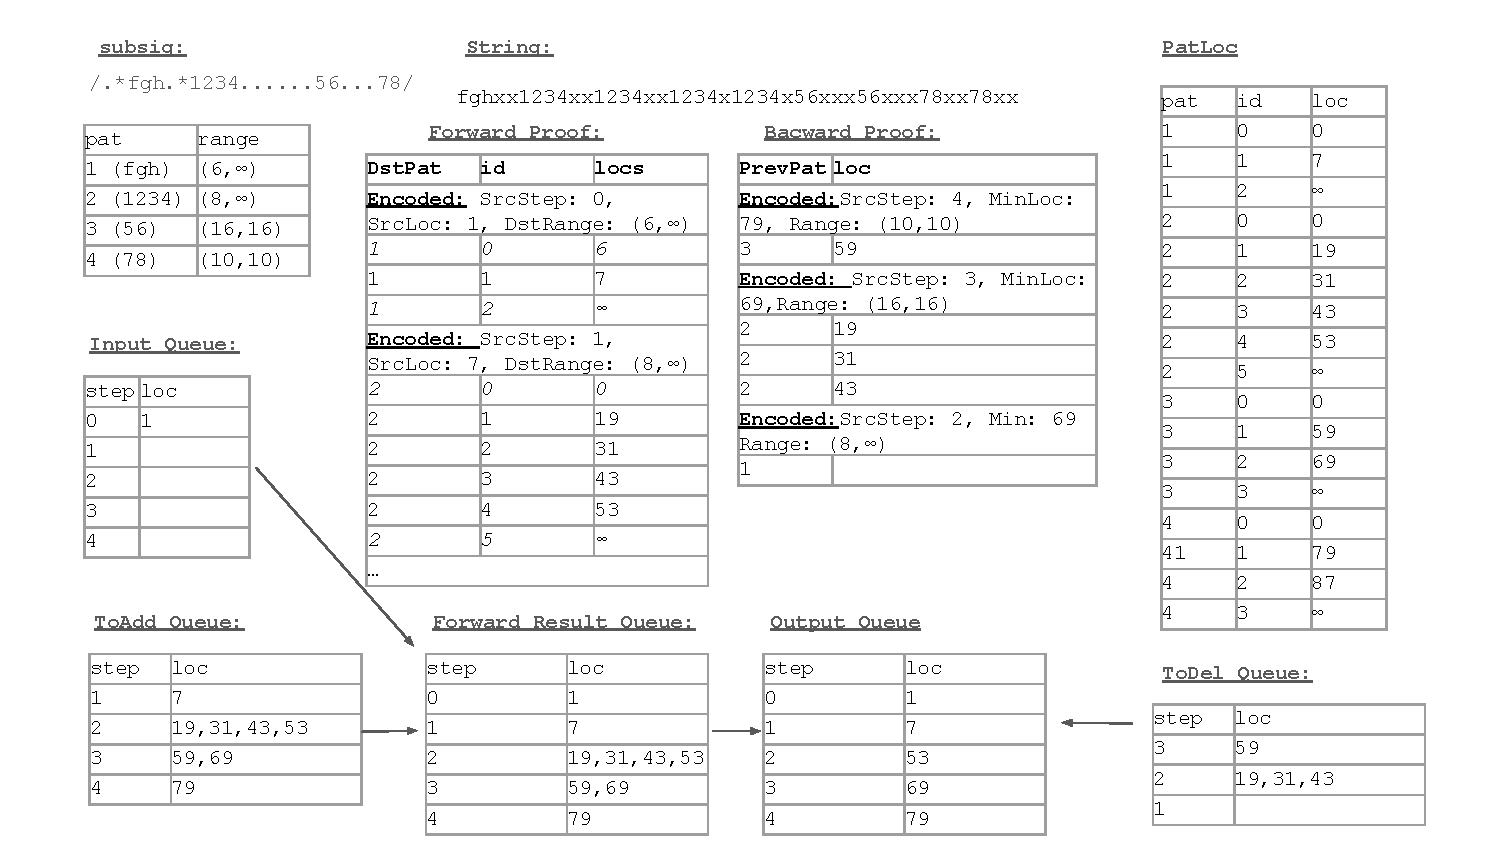
\includegraphics[width=\textwidth]{figs/FwdBwd.pdf}
\caption{Streaming Workflow for Foward and Backward Pruning}
\label{fig_stream}
\end{figure*}

\subsection{Streaming Algorithm for SED}
We now present the streaming algorithm for SED. We show how to use
internal lookups to support relational database operations needed.

We start with an informal introduction and a motivating example.
Recall that SED tries to discharge a string $s$ against 
a regex subsignature $r$ by checking the distance between patterns
of $r$. In Figure \ref{fig_stream}, we show an example
of regex which consists of four patterns (``fgh", ``1234", ``56", and ``78"). 
Each pattern has an expected range of distance from the match of
a previous pattern. For instance, the distance between ``1234" and ``56"
should be 16 nibbles (i.e., 8 characters, because the length of ``56"
is also counted).

SED has a pre-compiled AC-DFA that corresponds to all these patterns.
Before running the forward-backward pruning algorithm, SED feeds
the given string to the ACDFA, gets the list of final states,
and then map these final states back to the corresponding pattern words.
As an example, the word ``fghxx1234..." in Figure \ref{fig_stream}
generates the ``PatLoc" table as shown. For instance, one can see
that pattern 2 occurs at locations (9, 13, 43, 53). Note that
the first location starts from 1, and each location accounts for one 
4-bit nibble.

Then SED maintains a StepQueue that records the list of locations
that correspond to each pattern (step) in the regex subsignature.
For instance, given the regex signature and input word in Figure \ref{fig_stream}, starting with an initial input queue (where location 1 for step 0
is included by default), it results in the Output Queue as shown 
in the figure.

The challenge of making the prover more eficient is that: we need
to eliminate those ``dead" locations from the step queue at run time.
We thus develop a forward-backward pruning algorithm. Consider the
following example.

\begin{example}
	Given the example in Figure\ \ref{fig_stream}. The forward process
first iteratively starts from each location of each step, identify
the applicable locations for the next step. For instance, given location 7
for step 1 (pattern 7), four locations of the next pattern (2) falls
into the range (within min-max distance (16,16): 19, 31, 43, 53.
Notice that the algorithm has to roll based on the ``on-going" result.
For step 3, it has to start from the newly generated locations (19, 31, 43, 53),
and identify the workable locations 59 and 69 for step 3 and so on.

   Once the forward process is done, we then run a backward pruning process
that removes ``dead" locations. Consider step 4, its current minimum
location is 79. Given that the distance between step 3 and 4 is 10,
this eliminates $59$ in step 3, because for new locations for step 4
added in the future, they can only be greater than 79 and for sure
there will be no new locations that can be derived from 59. Thus
59 should be removed from the location list of step 3. Similalry,
the new ``min-loc" for step 3 now becomes 69, and this eliminates
19, 31, 43 from step 2. The list to delete is shown in ``ToDel Queue"
in Figure \ref{fig_stream}, which results in the final Output Queue.
\end{example}

\section{zkSnark Design}
\subsection{Overview}
This section introduces 
\foldpot,
an efficient folding scheme
that is tailored for efficiently verifying
the discharging algorithms introduced earlier.
\foldpot, as its name suggests, mixes
the design from several
recent folding schemes, including
SuperNova \cite{SuperNova}, \footnote{SuperNova uses a linear
folding model as Nova \cite{Nova}. 
Here we assume heuristically
that there is no known attack over the number of steps being folded.
In \cite[Remark 6.3]{BCCT13}, it was pointed out that stronger assumption on
extractor size/time extractor (e.g., additive over prover) leads
to polynomial step bound (instead of the constant bound if
assuming polynomial extractor for a general SNARK scheme for each step
in a recursive SNARK composition scheme).
This was shown in recent workk \cite{AGMRecursion}.
It gives a contrived example
which shows that when blackbox knowledge extractor run time becomes
superpolynomial after $\log(\lambda)$ steps, soundness can be broken.
However, it also shows that under a modified AGM model (where prover keys
are uniformly distributed), Nova/SuperNova is secure given that
Pedersen vector commitment is used. Here
we use the sequential folding scheme for the problem size
we deal with, which incurs maximum $2^{17}$ steps, though
PCD tree based folding/accuulation is possible with further
development work.}
Cyclefold \cite{CycleFold}, Mangrove \cite{Mangrove} as well as
finger-printing schemes such as Mirage+ \cite{AIPRam}, and the
idea of NARK compiler from ProtoStar \cite{ProtoStar}.
We also assilate the idea of finger-printing techniques,
which were practiced in many previous works \cite{Mirage,AIPRam,Zkreg},
and adapt it in the folding schemes.

We first introduce the design goals that lead to the design
of \foldpot.  First, we would like to discharge a 
large collection of files (e.g., all Linux
executables). It is known that folding/accumulation 
provides an overall more efficient solution
than proof agregation schemes SNARKPack \cite{SNARKPack} 
and GIPA \cite{Bunz21} both asympototically (at verifier) and
concretely (at prover). Given that discharging of each individual file
needs to stack discharging steps non-uniformly,
we decide to adopt SuperNova \cite{SuperNova} for its 
support of non-uniform sub-circuits. It is appealing to provide
concretely small and constant size proof, especially verifiable
on-chain (e.g., ETH), CycleFold \cite{CycleFold} provides
an efficient decider proof generation over half pairing groups
BN254 + Grumpkin, so that $O(1)$ final decider proof can be
generated over BN254.
Finally, the system relies heavily on finger-printing techniques,
and our circuit model adapts the one from Mirage+ \cite{AIPRam}.
We then integrate the idea of commit-and-fold from 
Mangrove \cite{Mangrove}: commitments of partial segment of
witnesses can be added into committed R1CS instance, and the check
can be delayed to final decider proof. Leveraging on Mangrove's
commit-and-fold scheme, we develop low-cost techniques for
passing data between non-uniform circuits.

Our contributions are: (1) A compressing scheme for interactive R1CS
model \cite{AIPRam} that results in less communication rounds (and hence
less recursion overhead); By instantiating the commit-and-fold
scheme in Mangrove \cite{Mangrove}, we are able to produce: 
(2) An efficient input/output passing scheme
between non-uniform step-circuits, which has considerable benefits
over general RAM techniques for streaming circuits; (3) 
A constant-size batching-proof protocol that handles the batch
proof problem for non-uniform problem statements. 

\subsection{Circuit Model}
To integrate the finger-printing technique in folding schemes,
we mix the I-R1CS model for Algebraic Interactive Protocol (AIP)
in \cite{AIPRam} and the commited R1CS relation of Nova/SuperNova
\cite{Nova}. The 
finger-printing technique divides witness into multiple segments, where
subsequent segments depend on the Fiat-Shamir public coin 
randoms that are generated from the hash of previous segments.
This technique has been widely deployed in real-world proving
systems such as Halo2 \cite{Halo2}.
The challenge here in folding
is that {\em the number of segments determines the number of
commitments}, which linearly increases the cost of the prover
for final decider. In our context,
one additional commitments costs at least
$5$ million R1CS per non-uniform circuit.
We therefore seek to reduce the number of segments,
and present a $\Sigma$-IR1CS model (which is a weaker model
than the general I-R1CS) but allows only one segment commitment.

We first motivate the model. Consider the $\cp$ algorithm, which
given an input word $s$, returns a collection of signatures
that cannot be discharged by $\cp$. The algorithm walks $s$
through ACDFA, from the acceptance path, extracts
a multi-set of acceptance states, compressing it into
a unique set, performing a join relation with a table that
maps from final states to signatures, and then converting 
the multi-set into a standard set. The algorithm can be
regarded as a sequential composition of a constant number
of component interactive protcols that heavily rely on
public-coin challenges from the verifier. For instance,
to prove two multi-sets $\myvec{a} \in \F^n$ and $\myvec{b} \in \F^n$ 
are permutation of each other, the verifier samples a challenge
$\beta$ and verifies, which is widely used, e.g., in lookup arguments
such as plookup \cite{plookup}:\footnote{CHECK TODO: see if this
ref is accurate}
\[
	\prod_{i=1}^n (\myvec{a}_i + \beta)  =
	\prod_{i=1}^n (\myvec{b}_i + \beta) 
\]

Such sequential composition of interactive protocols is
nicely captured by the notion of AIP and I-R1CS \cite{AIPRam},
where an I-RICS instance has a constant number of message
exchanges, and a final R1CS check (which is similar to the
NARK verifier in ProtoStar \cite{ProtoStar}, with the
restriction of degree $2$). 
In \cite{AIPRam}, the multi-round interaction is handled
by a multi-segment variation of Groth16 \cite{Groth16}
and commit-and-prove extension of Mirage \cite{Mirage}, because
verifier can perform the Fiat-Shamir to generate public coin
challenges out-of-circuit.

In our context, the circuit has to be folded. Generating a commitment
for each round of messages to be exchanged is expensive, because
it increases recursion overhead. Instead, we use a 
restricted I-R1CS (called $\Sigma$-I-R1CS) that consists of
only two messages from the prover to verifier, one at
the beginning, consisting of the concatenation of problem statements
and all messages that are independent of public coins, and
the last message consists of all intermediate messages that
depend on random challenges. We show that a restricted AIP bound by
a certain ``join" property can always be
compiled into a 3-move I-R1CS, and then using the 
ProtoStar compiler \cite{ProtoStar}, compiled into a NARK.
We motivate our construction using an example.

\begin{example} \label{examp:ir1cs}
Assume there is a lookup table $\myvec{T} \subseteq \F$ which defines
a range that excludes $0$ (e.g., a set of final states of an ACDFA,
which ranges from $1$ to $2^{k}-1$ for some $k$).
Given $\myvec{a} \in \myvec{T}^{m}$ and $\myvec{b} \in \myvec{T}^n$,
consider the task of proving that $\myvec{a}$ is the {\em set support}
of multi-set $\myvec{b}$, that is: $\myvec{a}$ includes all the elements of
$\myvec{b}$, and $\myvec{b}$ includes all of $\myvec{a}$, and there is no duplicate element in $\myvec{a}$, assuming that all elements of
$\myvec{a}$ and $\myvec{b}$ belong to $\myvec{T}$.

We can denote it as a relation 
$(\myvec{a}, \myvec{b}, \myvec{T}; \myvec{w}) \in R$, where
a four element tuple $(m,n,2^{k}-1, 0)$ defines $R$'s structure (length
of each message vector).
Here $\myvec{a}$, $\myvec{b}$, $\myvec{T}$ are the
problem statement that 
is visible by both the prover and verifier.
$\myvec{w}$ (separated using \texttt{;} from the statement)
is the secret witness of prover. For this example,
$\myvec{w} = \emptyset$.
We call $R$ an {\em algebraic relation with a fixed structure} 
as all elements involved
in the relation are field elements.\footnote{We note that 
group elements can always be represented non-natively given a 
target field by bit-splitting.} 
We sometimes write $(\myvec{a}, \myvec{b}, \myvec{T}) \in R$
for short when context is clear.

Note that relation $R$ has an interesting property: it is a 
{\em natural join} of three 
relations: $R_1$, $R_1'$, and $R_2$. Here, 
$R_1(\myvec{x},\myvec{y};\myvec{w}_1)$ asserts a lookup relation
that all elements of $\myvec{x}$ belongs to $\myvec{y}$.
$R_1'$ is exactly the same as $R_1$ except changing
the config by swapping the size of the first 
two problem statement elements.
$R_2(\myvec{x}, \myvec{T};\myvec{w}_2)$ asserts that
all elements of $\myvec{x}$ are unique (assuming all 
$\myvec{x}_i \in \myvec{T}$).
Apparently $(\myvec{a}, \myvec{b}, \myvec{T}) \in R$ if and only if 
there exists $\myvec{w}_1$, $\myvec{w}_2$, and $\myvec{w}_3$ s.t.
$\myvec(\myvec{a}, \myvec{b}; \myvec{w}_1) \in R_1$,
$\myvec(\myvec{b}, \myvec{a}; \myvec{w}_1) \in R_1$,
and $\myvec(\myvec{a}, \myvec{T}; \myvec{w}_2) \in R_2$.\footnote{In 
real implementation, we allow $\myvec{a}$ and $\myvec{b}$ to
contain $0$ as dummy filler elements to make the circuits
more general purpose at slightly more constriant cost.}

For $R$, each of its sub-relation has a constant move special
sound protocol (similar to those defined in ProtoStar \cite{ProtoStar}).
For instance, Consider $R_1$, it has a $3$-move special sound protocol
by \cite{Hab22}, as shown in $\proto_1$ in Figure \ref{fig:2shots}. 
Similarly, let $\proto_1'$ be the protocol for $R_1'$.
Its basic idea
is that if the lookup relation holds, the sum of logarithmic derivative
of the elements of two vectors will match. Protocol
$\proto_2$ for $R_2$ is essentially running $\proto_1$ to prove
that the difference for each pair of elements of $\myvec{x}$ is
a positive integer, excluding $0$ (because $0 \not\in \myvec{T}$),
thus proving $\myvec{x}$ is sorted in ascending order, hence
a set without duplicates. One can see that each corresponds to
an I-R1CS protocol where a degree $2$ function is performed
at the end for making checks. It is known that degree $2$ functions
can be expressed in R1CS.

Sequential composition of these protocols is costly in folding.
Instead, we can compile them into $\proto$ as shown in Figure\ \ref{fig:2shots}.
Basically, it combines all the first message from all sub-protocols
in its first message, keeping the structure of public coin verifier
challenges, and then combine all ``response" messages from sub-protocols
in one last message, and then projecting each individual messages
from the combined messages, and run the degree $2$ check functions
correspondingly.  We call this compiled protocol {\em $\Sigma$-I-R1CS} 
because it has 3 moves.

We can then apply the comiler technique in ProtoStar
\cite[Section 3.2]{ProtoStar}, to compile a
$\Sigma$-I-R1CS into a committed protocol
by sending commitments of the first and
third message, and add additional checks to open them (as shown in
$\proto_{\textrm{cm}}$ in Figure\ \ref{fig:2shots}).
One might wonder why sending the commitments and then
immediately open them up. The reason is that these commitments
are included as part of the committed instances
to be folded, and the opening check only performed at the final decider proof,
{\em only once} for many instances that are folded.
\end{example}

Let $\rohash$  denotes the hash function to instantiate 
the random-oracle.
We summarize our discussion and the main finding below.

\begin{definition} An algebraic relation $R$ is an NP relation
over $\F$ with a fixed structure.
We call $R(\myvec{x})$ {\em decomposible by joins} of a constant number of
relations $R_1, ... R_k$ if all of the following
are satisfied:
(1) Each $R_i$ has a special-sound
$\Sigma$-protocol, and
(2) Denote $\myvec{x}$ as $\myvec{x}^{(k+1)}$.
There exists a join function $\varphi$ s.t.
$\varphi$ is a DNF (disjunctive normal form) of 
equality constraints of form $\myvec{x}^{(i)}_u = \myvec{x}^{(j)}_v$,
where $0\leq i,j \leq k+1$.
For any $(\myvec{x}, \myvec{w})$:
$(\myvec{x}; \myvec{w}) \in R$ if and only if
there exists 
$(\myvec{x}^{(1)}; \myvec{w}^{(1)}) \in R_1$,
$(\myvec{x}^{(2)}; \myvec{w}^{(2)}) \in R_2$,
...
$(\myvec{x}^{(k)}; \myvec{w}^{(k)}) \in R_k$, 
and $\varphi(\myvec{x}^{(1)}, ..., \myvec{x}^{(k)},\myvec{x}) = \texttt{true}$.
\end{definition}

We note that there can be more expressive form of expressing the
join relation $\varphi$, but this form sufficies for our applications.
Note that $\varphi$ is degree $1$, hence it can be encoded in R1CS.

\begin{figure*}
%\resizebox{4.5in}{4.5in}{
\resizebox{0.90\textwidth}{!}{
	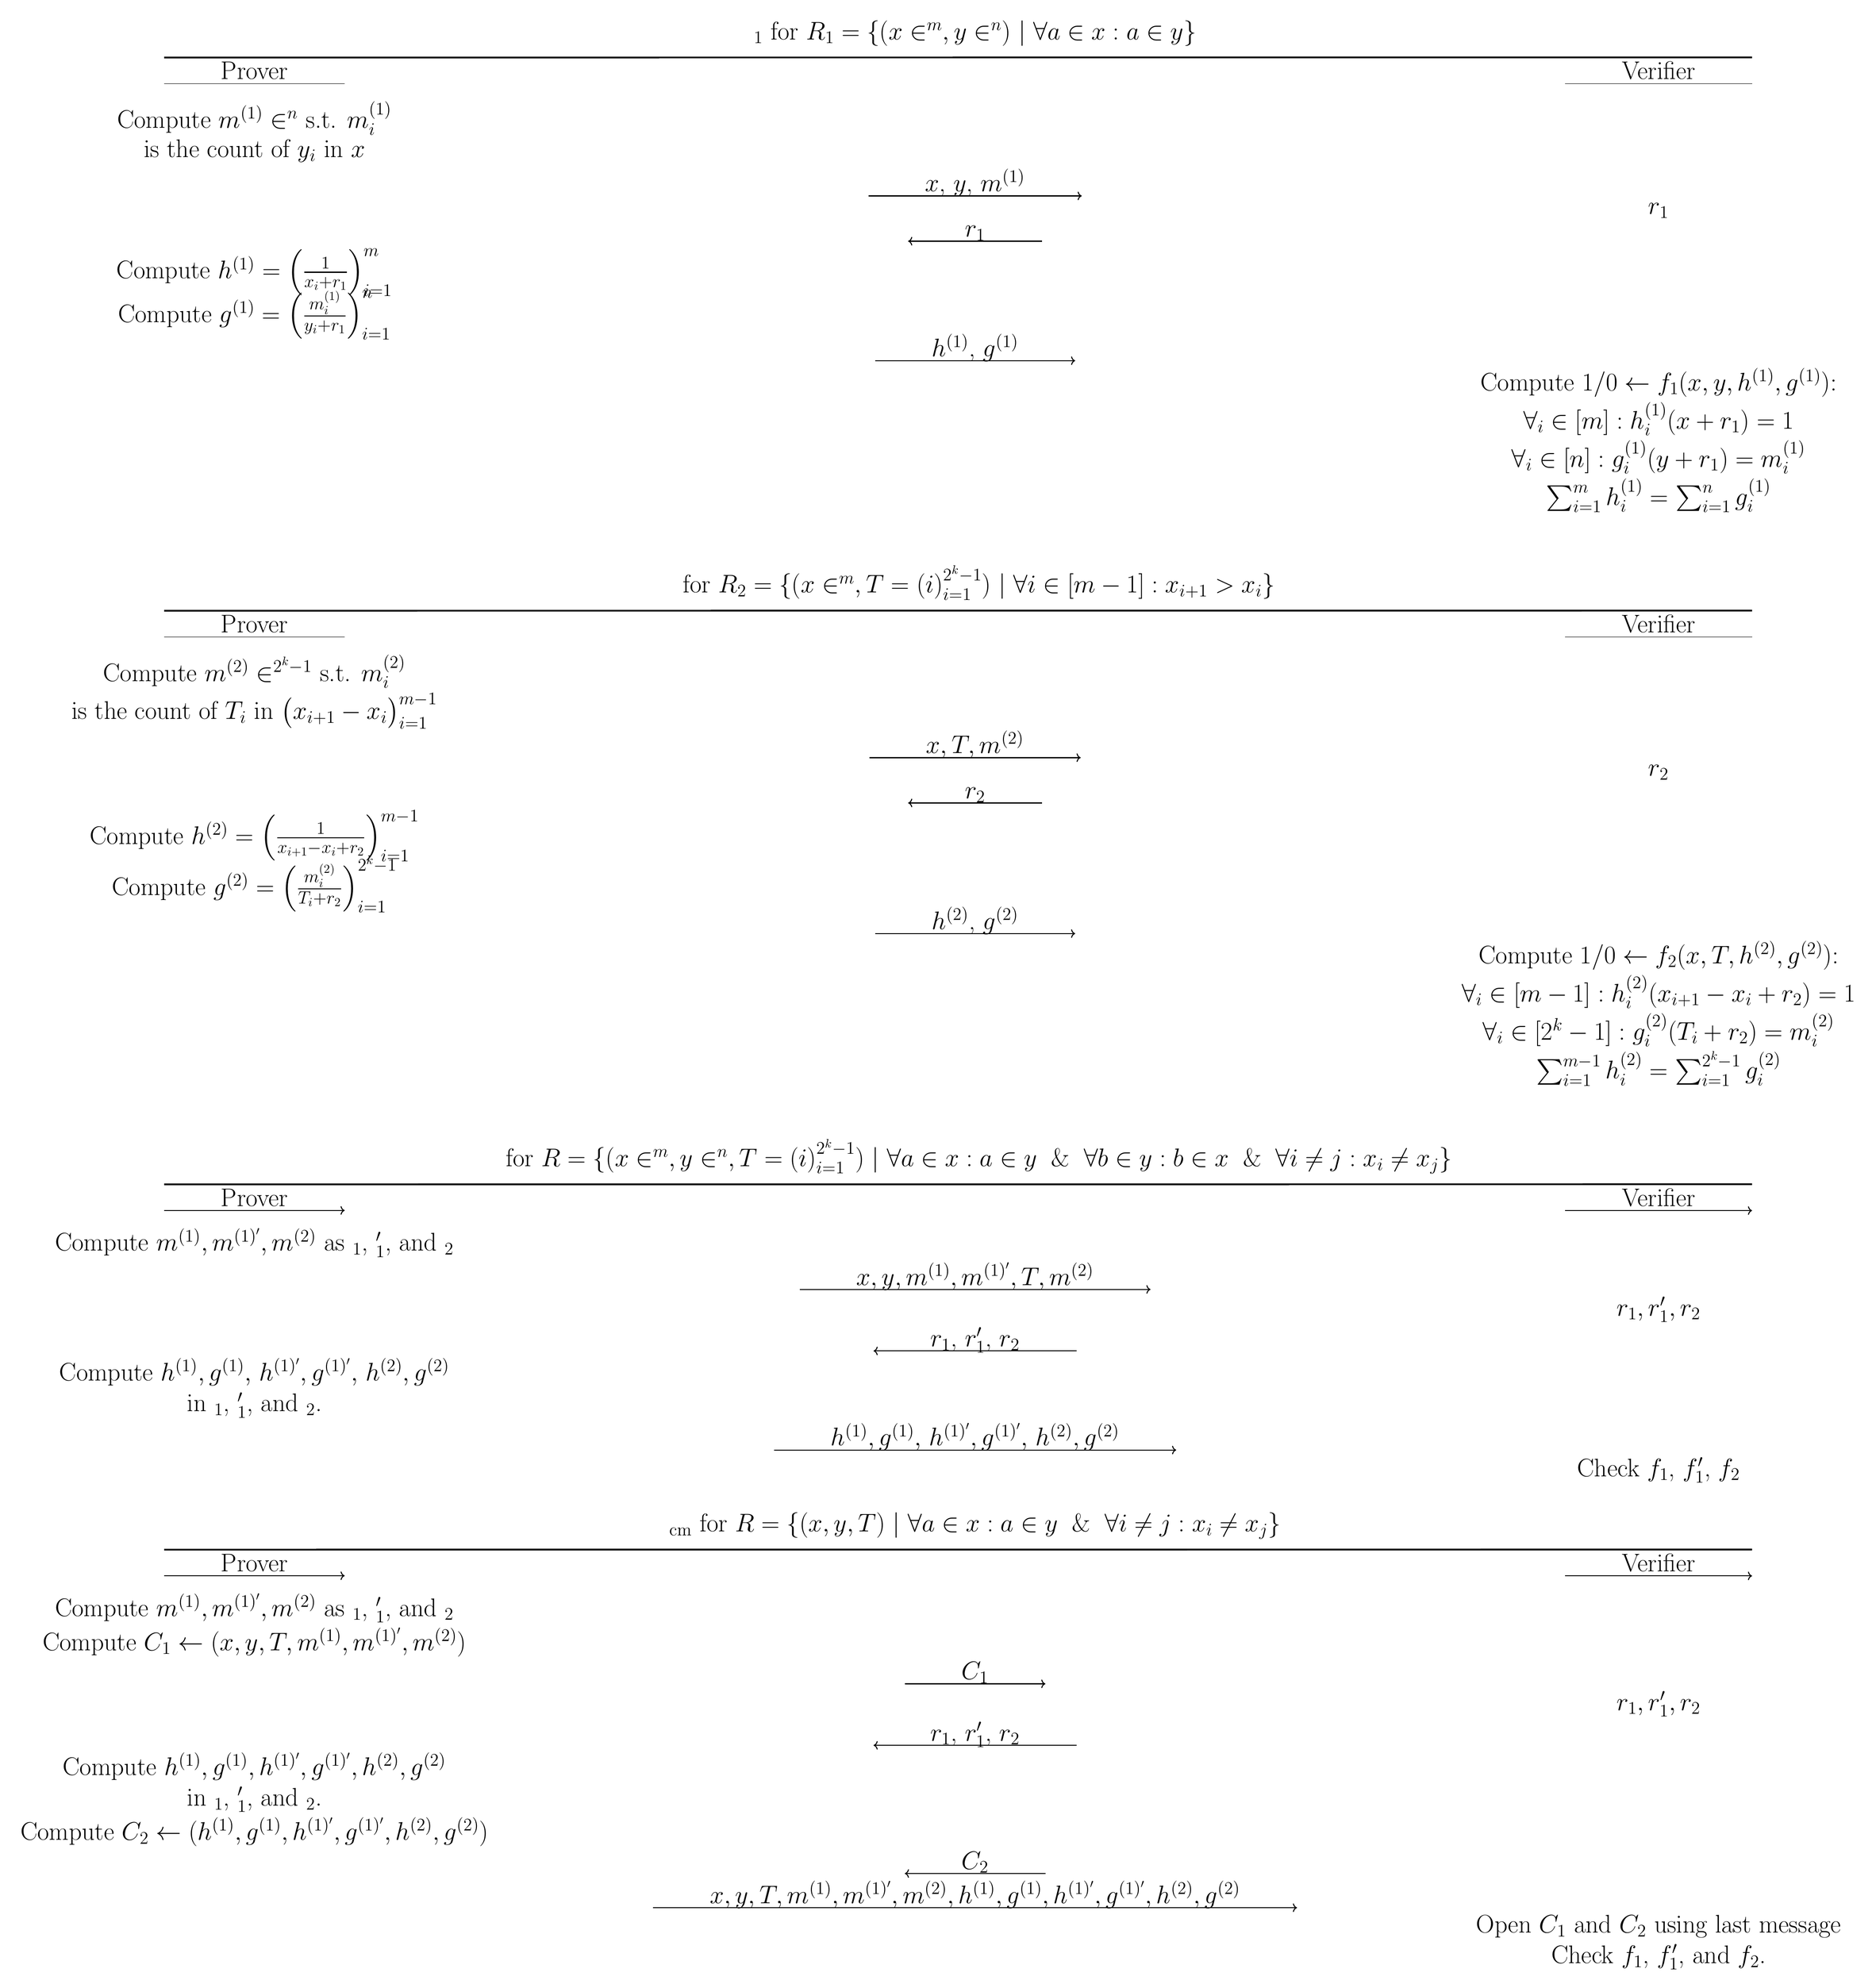
\begin{tikzpicture}
 \tikzstyle{every node}=[font=\fontsize{20}{20}\selectfont]
\matrix (m)[matrix of nodes, column sep=0.5mm,row  sep=8mm, nodes={draw=none, anchor=center,text depth=0pt} ]{
 %row 1 
 & $\proto_1$ for $R_1 = \{(\myvec{x}\in \F^{m},\myvec{y}\in \F^{n}) ~|~\forall a\in \myvec{x}: a\in \myvec{y} \}$ & \\[-4mm]
 %row 2 
 Prover & & Verifier\\[-4mm]
 %row 3
 Compute $\myvec{m}^{(1)} \in \F^n$ s.t. $\myvec{m}^{(1)}_i$ & & \\ [-7mm]
 %row 4
 is the count of $\myvec{y}_i$ in $\myvec{x}$ & &  \\ [-7mm]
 %row 5
 & $\myvec{x}$, $\myvec{y}$, $\myvec{m}^{(1)}$ & \\  [-7mm]
 %row 6
 & & $r_1 \pick \F$ \\ [-7mm]
 %row 7
 & $r_1$ & \\ [-7mm]
 %row 8
 Compute $\myvec{h}^{(1)} = \left(\frac{1}{\myvec{x}_i+r_1}\right)_{i=1}^m$ & & \\ [-7mm]
 %row 9
 Compute $\myvec{g}^{(1)} = \left(\frac{\myvec{m}^{(1)}_i}{\myvec{y}_i+r_1}\right)_{i=1}^n$ & & \\ [-7mm]
 %row 10 
 & $\myvec{h}^{(1)}$, $\myvec{g}^{(1)}$ & \\ [-7mm]
 %row 11 
 & & Compute $1/0 \leftarrow f_1(\myvec{x}, \myvec{y}, \myvec{h}^{(1)}, \myvec{g}^{(1)})$: \\ [-7mm]
 %row 12 
 &  & $\forall_i\in [m]: \myvec{h}^{(1)}_i(\myvec{x}+r_1) = 1$ \\ [-7mm]
 %row 13 
 & & $\forall_i\in [n]: \myvec{g}^{(1)}_i(\myvec{y}+r_1) = \myvec{m}^{(1)}_i$ \\ [-7mm]
 %row 14 
 & & $\sum_{i=1}^m \myvec{h}^{(1)}_i = \sum_{i=1}^n \myvec{g}^{(1)}_i$  \\[7mm]
 %row 15 
 & $\proto$ for $R_2 = \{(\myvec{x}\in \F^{m},\myvec{T}=\left(i\right)_{i=1}^{2^k-1}) ~|~\forall i\in [m-1]: \myvec{x}_{i+1}>\myvec{x}_{i} \}$ & \\[-4mm]
 %row 16 
 Prover & & Verifier\\[-4mm]
 %row 17 
 Compute $\myvec{m}^{(2)} \in \F^{2^{k}-1}$ s.t. $\myvec{m}^{(2)}_i$ & & \\ [-7mm]
 %row 18 
 is the count of $\myvec{T}_i$ in $\big(\myvec{x}_{i+1}-\myvec{x}_{i}\big)_{i=1}^{m-1}$ & &  \\ [-7mm]
 %row 19 
 & $\myvec{x}, \myvec{T}, \myvec{m}^{(2)}$ & \\ [-7mm]
 %row 20 
 & & $r_2 \pick \F$ \\ [-7mm]
 %row 21 
 & $r_2$ & \\ [-7mm]
 %row 22 
 Compute $\myvec{h}^{(2)} = \left(\frac{1}{\myvec{x}_{i+1}-\myvec{x}_{i}+r_2}\right)_{i=1}^{m-1}$ & & \\ [-7mm]
 %row 23 
 Compute $\myvec{g}^{(2)} = \left(\frac{\myvec{m}^{(2)}_i}{\myvec{T}_i+r_2}\right)_{i=1}^{2^k-1}$ & & \\ [-7mm]
 %row 24 
 & $\myvec{h}^{(2)}$, $\myvec{g}^{(2)}$ & \\ [-7mm]
 %row 25 
 & & Compute $1/0 \leftarrow f_2(\myvec{x}, \myvec{T}, \myvec{h}^{(2)}, \myvec{g}^{(2)})$: \\ [-7mm]
 %row 26 
 &  & $\forall_i\in [m-1]: \myvec{h}^{(2)}_i (\myvec{x}_{i+1} - \myvec{x}_{i} +r_2) = 1$ \\ [-7mm]
 %row 27 
 & & $\forall_i\in [2^k-1]: \myvec{g}^{(2)}_i (\myvec{T}_{i}+r_2) = \myvec{m}^{(2)}_i$ \\ [-7mm]
 %row 28 
 & & $\sum_{i=1}^{m-1} \myvec{h}^{(2)}_i = \sum_{i=1}^{2^k-1} \myvec{g}^{(2)}_i$  \\[7mm]
 %row 29 
 & $\proto$ for $R = \{(\myvec{x}\in \F^{m},\myvec{y}\in \F^{n},\myvec{T}=\left(i\right)_{i=1}^{2^k-1}) ~|~\forall a\in \myvec{x}: a\in \myvec{y} \And \forall b\in \myvec{y}: b\in \myvec{x} \And \forall i\neq j: \myvec{x}_i \neq \myvec{x}_j\}$ & \\[-4mm]
 %row 30 
 Prover & & Verifier\\[-4mm]
 %row 31 
 Compute $\myvec{m}^{(1)}, \myvec{m}^{(1)'}, \myvec{m}^{(2)}$ as $\proto_1$, $\proto_1'$, and $\proto_2$ & & \\ [-7mm]
 %row 32
 & $\myvec{x}, \myvec{y}, \myvec{m}^{(1)}, \myvec{m}^{(1)'}, \myvec{T}, \myvec{m}^{(2)}$ & \\[-7mm]
 %row 33
 & & $r_1, r_1', r_2 \pick \F$ \\[-7mm]
 %row 34
 & $r_1$, $r_1'$, $r_2$ & \\[-7mm]
 %row 35
 Compute 
 $\myvec{h}^{(1)}, \myvec{g}^{(1)},$ 
 $\myvec{h}^{(1)'}, \myvec{g}^{(1)'},$ 
 $\myvec{h}^{(2)}, \myvec{g}^{(2)}$ & & \\[-7mm]
 %row 36
 in $\proto_1$, $\proto_1'$, and $\proto_2$. & & \\[-7mm]
 %row 37
 & 
 	$\myvec{h}^{(1)}, \myvec{g}^{(1)},$
 	$\myvec{h}^{(1)'}, \myvec{g}^{(1)'},$ 
	$\myvec{h}^{(2)}, \myvec{g}^{(2)}$ & \\[-7mm]
 %row 38
 & & Check $f_1$, $f_1'$, $f_2$  \\
 %row 39  ----- Committed Protocol
 & $\proto_{\textrm{cm}}$ for $R = \{(\myvec{x},\myvec{y},\myvec{T}) ~|~\forall a\in \myvec{x}: a\in \myvec{y} \And \forall i\neq j: \myvec{x}_i \neq \myvec{x}_j\}$ & \\[-4mm]
 %row 40 
 Prover & & Verifier\\[-4mm]
 %row 41 
 Compute $\myvec{m}^{(1)}, \myvec{m}^{(1)'}, \myvec{m}^{(2)}$ as $\proto_1$,
  $\proto_1'$, and $\proto_2$ & & \\ [-7mm]
 %row 42
 Compute $C_1 \leftarrow \com(\myvec{x}, \myvec{y}, \myvec{T}, \myvec{m}^{(1)}, \myvec{m}^{(1)'}, \myvec{m}^{(2)})$  & & \\ [-7mm]
 %row 43
 & $C_1$ & \\[-7mm]
 %row 44 
 & & $r_1, r_1', r_2 \pick \F$ \\[-7mm]
 %row 45 
 & $r_1$, $r_1'$, $r_2$ & \\[-7mm]
 %row 46 
 Compute $\myvec{h}^{(1)}, \myvec{g}^{(1)}, 
 \myvec{h}^{(1)'}, \myvec{g}^{(1)'}, 
 	\myvec{h}^{(2)}, \myvec{g}^{(2)}$ & & \\[-7mm]
 %row 47 
 in $\proto_1$, $\proto_1'$, and $\proto_2$. & & \\[-7mm]
 %row 48
 Compute $C_2 \leftarrow \com(\myvec{h}^{(1)}, \myvec{g}^{(1)}, 
 	\myvec{h}^{(1)'}, \myvec{g}^{(1)'}, 
	\myvec{h}^{(2)}, \myvec{g}^{(2)})$ & & \\[-7mm]
 %row 49 
 & $C_2$ & \\[-7mm]
 %row 50 
 & $\myvec{x}, \myvec{y}, \myvec{T}, \myvec{m}^{(1)}, \myvec{m}^{(1)'}, 
 \myvec{m}^{(2)}, \myvec{h}^{(1)}, \myvec{g}^{(1)}, 
 \myvec{h}^{(1)'}, \myvec{g}^{(1)'}, 
 \myvec{h}^{(2)}, \myvec{g}^{(2)}$ & \\[-7mm]
 %row 51 
 & & Open $C_1$ and $C_2$ using last message \\[-7mm]
 %row 52 
 & & Check $f_1$, $f_1'$, and $f_2$.  \\[-7mm]
};
\draw[line width=0.50mm,shorten <=-1.5cm,shorten >=-1.5cm] (m-2-1.north west)--(m-2-3.north east);
\draw[shorten <=-1.5cm,shorten >=-1.5cm] (m-2-1.south east)--(m-2-1.south west);
\draw[shorten <=-1.5cm,shorten >=-1.5cm] (m-2-3.south east)--(m-2-3.south west);
\draw[shorten <=-1.5cm,shorten >=-1.5cm,->,thick,black] (m-5-2.south west)--(m-5-2.south east);
%\draw[-{latex[length=3mm,width=5mm]}] (m-5-2.south west)--(m-5-2.south east);
\draw[shorten <=-1.5cm,shorten >=-1.5cm,->,thick,black] (m-7-2.south east)--(m-7-2.south west);
\draw[shorten <=-1.5cm,shorten >=-1.5cm,->,thick,black] (m-10-2.south west)--(m-10-2.south east);
\draw[line width=0.50mm,shorten <=-1.5cm,shorten >=-1.5cm] (m-16-1.north west)--(m-16-3.north east);
\draw[shorten <=-1.5cm,shorten >=-1.5cm] (m-16-1.south east)--(m-16-1.south west);
\draw[shorten <=-1.5cm,shorten >=-1.5cm] (m-16-3.south east)--(m-16-3.south west);
\draw[shorten <=-1.5cm,shorten >=-1.5cm,->,thick,black] (m-19-2.south west)--(m-19-2.south east);
\draw[shorten <=-1.5cm,shorten >=-1.5cm,->,thick,black] (m-21-2.south east)--(m-21-2.south west);
\draw[shorten <=-1.5cm,shorten >=-1.5cm,->,thick,black] (m-24-2.south west)--(m-24-2.south east);
\draw[line width=0.50mm,shorten <=-1.5cm,shorten >=-1.5cm] (m-30-1.north west)--(m-30-3.north east);
\draw[shorten <=-1.5cm,shorten >=-1.5cm,->,thick,black] (m-30-1.south west)--(m-30-1.south east);
\draw[shorten <=-1.5cm,shorten >=-1.5cm,->,thick,black] (m-30-3.south west)--(m-30-3.south east);
\draw[shorten <=-1.5cm,shorten >=-1.5cm,->,thick,black] (m-32-2.south west)--(m-32-2.south east);
\draw[shorten <=-1.5cm,shorten >=-1.5cm,->,thick,black] (m-34-2.south east)--(m-34-2.south west);
\draw[shorten <=-1.5cm,shorten >=-1.5cm,->,thick,black] (m-37-2.south west)--(m-37-2.south east);
%--- prot_cm
\draw[line width=0.50mm, shorten <=-1.5cm,shorten >=-1.5cm,] (m-40-1.north west)--(m-40-3.north east);
\draw[shorten <=-1.5cm,shorten >=-1.5cm,->,thick,black] (m-40-1.south west)--(m-40-1.south east);
\draw[shorten <=-1.5cm,shorten >=-1.5cm,->,thick,black] (m-40-3.south west)--(m-40-3.south east);
\draw[shorten <=-1.5cm,shorten >=-1.5cm,->,thick,black] (m-45-2.south east)--(m-45-2.south west);
\draw[shorten <=-1.5cm,shorten >=-1.5cm,->,thick,black] (m-43-2.south west)--(m-43-2.south east);
\draw[shorten <=-1.5cm,shorten >=-1.5cm,->,thick,black] (m-49-2.south east)--(m-49-2.south west);
\draw[shorten <=-1.5cm,shorten >=-1.5cm,->,thick,black] (m-50-2.south west)--(m-50-2.south east);
\end{tikzpicture}

}
\caption{Protocols for Example \ref{examp:ir1cs}}
\label{fig:2shots}
\end{figure*}

\begin{lemma}\label{lemma:ir1cs}
Let $R$ be a decomposable relation joined by
$k$ sub-relations with special-sound $\Sigma$-protocols.
There exists a $3$-move
special-sound I-R1CS protocol for $R$. 
\end{lemma}

\begin{proof} 
We use $\proto_s(R)$ to denote the I-R1CS protocol that sequentially
composes all $k$ sub-protocols of $R$, which performs
the check of join relation $\phi$ and the R1CS checks for
all of the sub-relations, and returns the conjunction of the Boolean
results. $\proto_s(R)$ is a complete and special-sound protocol
for $R$, and it has $3k$ moves.

We use $\proto_p(R)$
to represent the $\Sigma$-protocol which is constructed by
sequentially concatenating the first messages of all 
subprotocols of $R$ for its first messages, and similarly
constructing its second and thrid messages.
$\proto_p(R)$ has $3$-moves. Its last R1CS module
performs the check of $\phi$ and the R1CS checks of all
sub-protocols.
It is apparent that for any transcript $\proto_s(R)$,
there is a one-to-one mapping $\Psi_R$ which uniquely
constructs a transcript for $\proto_p(R)$. $\Psi_R$ can 
be directly inferred from the structure information of $R$
and its sub-protocols.

It is not hard to see that $\proto_s(R)$ and $\proto_p(R)$
are equivalent, in the sense that, for an accepted transcript $t$ 
of $\proto_s(R)$, its $\Psi_R(t)$ is also accepted by $\proto_p$;
vice versa for the inverse relation $\Psi_R^{{-1}}$.
An ``invalid" transcript (which falsely proves a 
$(\myvec{x};\myvec{w}) \not\in R$
is in $R$) has negilible probability of passing $\proto_s(R)$,
and also for $\proto_p(R)$. The soundness error of the two protcols
are the same, both linearly degrading with the number of sub-protocols,
because the R1CS check modules of the two are equivalent.

When Fiat-Shamir is applied to $\proto_p(R)$,
the soundness loss {\em independent} of the number of public coin verifier 
challenges, per \cite{SpecialFiat}.
\end{proof}

We note that our I-R1CS model (even extended to more than
$3$ messages) is a strictly (restrictive) weaker 
than the original I-R1CS \cite{AIPRam}. The key difference is that, by 
the restriction of ``join" relation, our model explicitly {\em enforces that
the second and third message of sub-protocols do not have
dependence on other sub-protocols}, only the claims of sub-protocols
might be related. This ``restriction" allows the projection between
$\proto_s(R)$ and $\proto_p(R)$. This model can still capture
a wide spectran of application scenarios, e.g., all of circuits
in our ZkregPlus system satisfy the condition. 
%and the same applies
%to the RAM protocols in \cite{AIPRam}.

\subsubsection{Lookup Table}
One drawback of the protocols presented in Figure\ \ref{fig:2shots}
is that if the lookup table size is much larger than the
statement vector, it is concretely very inefficient. We provide
two solutions for the problem. 

One solution, when the total
prover work is small (e.g., very small number of folding steps
or in the case of no folding), one can use commit-and-prove approach
to take out the commitment of all elements that need to perform
lookups, and then outside of the circuit, run an independent
zero knolwedge lookup protocol. As the lookup table is fixed for
our application scenario, it can be pre-processed. We provide
a zero knowledge version of the CQ protocol \cite{cq} in Appendix 
\ref{apdx:zk_cq}, as an contribution of independent interst.
In this case, the prover only has to pay a concrete cost
of the query table size (which is indpepenent of the size of
the container table). The protocol in \ref{apdx:zk_cq}
can be replaced by the zk-cq protocol in \cite{MatrixLookup},
which has slightly smaller proof size but higher prover cost than our
protocol.

The second solution is to adopt the commit-and-fold scheme presented in 
Mangrove \cite{Mangrove}. When the total prover work (e.g., folding
$2^{17}$ circuits of an average circuit size of $2^{16}$ each,
a lookup table of $2^{28}$ can be distributed into each step, 
incurring a negligible cost of about $3\%$). We adopt the Mangrove approach
in our implementation for its convenience. 
We note that the folding lookup scheme in ProtoStar \cite{ProtoStar} yields
similar asympototic and estimated similar concrete performance.

There is one more issue to consider: for the ZkregPlus system,
there are many individual look-up tables. Range proofs are all
achieved using lookups, and there are several different
types of range proofs: ACDFA states are $23$ bits,
input alphabet is $4$-bit, and signature IDs are $16$ bits.
The $\cp$ approach needs 2 ACDFAs, one for case insensitive and
one for case sensitive. The $\bw$ and $\sde$ combined,
needs 2 more ACDFAs.  In total, these $4$ ACDFAs, have
about $160$ million transtions, to be encoded in four separate
look-up tables. We also need to encode the $\bw$ and $\sde$
discharging instructions separately.  

We put all these separate tables into one $2$-column look-up table,
with first column indicates the sub-table ID, and the second column
indicates the value. We reserve $0$ as $\texttt{null}$
sub-table ID. The logarithmic derivative approach 
\cite{Hab22,cq,ProtoStar} supports multi-column table well.

Putting all ingredients together, we now have the formal
definition of $\Sigma$-I-R1CS enriched with lookup. It is
used to specify the step-circuit in FoldPot, essentially
adopting the SuperNova \cite{SuperNova} + CycleFold \cite{CycleFold}.
This definition is adapted from \cite[Definition 1]{AIPRam}.

\begin{definition} \label{deff:ir1cs}  
A $\Sigma$-I-R1CS is a tuple $\phi$ defined
as below:
\[
(N, n, \F; \myvec{T} \in \F^{N\times 2}, 
\ell_x, \ell_{m_1}, \ell_{m_2}, \ell_{m_3} \in \nat; 
A,B,C \in \F^{n\times m}; \chi)
\]
Here $\myvec{T}$ is a pre-processed 2-column look-up table.
$\chi: \nat \rightarrow \nat$ is a function that maps
a variable index to a sub-table ID in $\myvec{T}$.
The protocol 
defines a 3-round AIP over $\F$. The prover sends the first (including
statement) and third message, and the verifier sends
the second message of uniformally sampled challenges.
Let $\myvec{x}$ be the statement, and $\big\{\myvec{m}^{(i)}\big\}_{i=1}^{3}$
be the three round of messages.
let $m$ = $\ell_x + \ell_{m_1} + \ell_{m_2} + \ell_{m_3}$.
The R1CS checker consists of three matrics $A, B, C$ of $n$ constraints.
Let $z = \myvec{x} \concat \myvec{m}^{(1)} \concat \myvec{m}^{(2)}
	\concat \myvec{m}^{(3)}$. 
The verifier accepts if $Az \circ Bz = Cz$, and
for each $i\in [m]:$ if $\chi(i) \neq \texttt{null}$ then
$(\chi(i), z_i) \in \myvec{T}$, i.e.,
$z_i$ is in sub-table $\chi(i)$.
\end{definition}

\subsection{Commit-and-Fold}
\label{cf_zksnark}
We now briefly review the commit-and-fold scheme proposed in
Mangrove \cite{Mangrove}, which we later instantiate to support
inter-circuit data passing and batch processing of non-uniform word
problems.

The base line of FoldPot is SuperNova \cite{SuperNova} and 
CycleFold \cite{CycleFold}, which solves non-uniformity of 
circuits in folding, and delivers
$O(1)$ proof. However, we still need to address the following challenges.

\begin{enumerate}
\item We need to handle large files (e.g., $2^{27}$ bytes) in
``streaming" mode. In this case, step-circuits need to pass
large amount of input/output data. We need a concretely
more efficient schemes than the general RAM approach (e.g., \cite{AIPRam}).

\item We need to discharge a collection of files in batch, and
then provide an individual (2-stage) proof for each file.
Given an aggregated word $\myvec{s}$ which is a concatenation
of $k$ segments, i.e.,
$\myvec{s} = \myvec{s}^{(1)} \concat \myvec{s}^{(2)} \concat ... \concat \myvec{s}^{(k)}$, and the individual commitments to each $\myvec{s}^{(i)}$,
we need to link these segment commitments with the $\myvec{s}$ in circuit,
and prove all of them malware free. Here the challenge is that
these word segments can have arbitrary length.
\end{enumerate}

We first present a simplified framework of Mangrove's 
commit-and-prove, in the context of committed R1CS used by Nova,
SuperNova and CycleFold, as all of our circuits are low-degree.
Recall the Nova \cite{Nova} framework: the folding prover
is given a running instance $(\myvec{U}_i; \myvec{W}_i)$ and an incoming (step)
instance $(\myvec{u}_i; \myvec{w}_i)$, where $\myvec{W}_i$ and 
$\myvec{w}_i$ are the witnessnes,
and fold them into a new instance $(\myvec{U}_{i+1}; \myvec{W}_{i+1})$. 
A folded instance is a tuple 
$(\overline{\myvec{W}}, \overline{\myvec{E}}, u, x)$,
where $u$ and $x$ are ``public" parameters of relaxed R1CS relation,
and $\overline{\myvec{W}}$ and $\overline{\myvec{E}}$ are homomorphic
commitments (e.g., Pedersen vector commitments) to the
witness and cross terms. The folding verifier in the IVC scheme
does not have to check the opening of $\overline{\myvec{W}}$ and 
$\overline{\myvec{E}}$ at each step. Instead, the 
check is {\em delayed} to the final decider proof,
and performed {\em only once} for all folded instances. 

The key observation made by Mangrove \cite{Mangrove} is that:
the committed instance can have extra commitments on subset of witnesses.
The opening of these commitments can be also delayed to the 
final decider step. Thus, if one performs a one pass aggregation (e.g.,
using Merkle tree) of these extra commitments, a commit-and-prove
scheme like LegoSNARK \cite{LegoSnark} can be achieved.  
In our context, the commitment to the subset of witness
can be used for generating the Fiat-Shamir randomness
and can be verified in-circuit.

In Mangrove, the formalization of commit-and-fold
was made using the polynomial relations, which supports high-degree.
We re-instate the result of Mangrove in the context of 2-degree R1CS
as below.
Given a $\Sigma$-I-R1CS instance $\phi$ whose
R1CS relation is $A,B,C \in \F^{n\times m}$, where
$m$ is the number of variables. Enrich $\phi$ with
$\rho$, a subset of $[0,m-1]$ sorted in ascending order.
Given the fixed size witness vector $\myvec{W}$, we
use $\rho(\myvec{W})$ to denote the projection of $\myvec{W}$ over
the indices included in $\rho$. For example, let
$\myvec{W} = (5, 30, 20, 1)$ and $\rho = (0, 2)$, then
$\rho(\myvec{W}) = (5, 20)$.
We denote the new $\Sigma$-I-R1CS instance as 
$\phi_{\rho}$.
The following defines relaxed and committed R1CS instance.
The difference from NOVA is the addition of the
projected commitments: $\overline{\rho(\myvec{W})}$.

\begin{definition} (extending \cite[Definition 12]{Nova})
\label{def:extr1cs}
A relaxed R1CS instance of $\phi_\rho$ consists
of $\myvec{A},\myvec{B},\myvec{C} \in \F^{n\times m}$ as in $\phi$,
an error vector $\myvec{E} \in \F^m$, and a scalar $u\in F$,
and input/output vector $\myvec{x} \in \F^{\ell}$.
Let $\myvec{z} = (\myvec{W}, \myvec{x}, u)$, and
$(\myvec{z}, \myvec{W^{(\rho)}})$ 
is accepted if $\myvec{A}\myvec{z} \circ \myvec{B}\myvec{z} 
= u(\myvec{C}\myvec{z}) + \myvec{E}$
and $\myvec{W^{(\rho)}} = \rho(\myvec{W})$. 
A committed R1CS instance for $\phi_\rho$ is a tuple 
$(\overline{\myvec{W}},$
$\overline{\myvec{E}}, u, \myvec{x}, \overline{\myvec{W^{(\rho)}}}$.
\end{definition}

The Nova/SuperNova folding schemes can be modified correspondingly.
When folding $\overline{\myvec{W}}$, $\overline{\myvec{W^{(\rho)}}}$ 
can be folded correspondingly (and in CycleFold, it can be fed
to a CycleFold circuit works on Grumpkin curve similarly). 
At the final decider, the verifier checks the 
folded $\myvec{W^{(\rho)}} = \rho(\myvec{W})$, 
and they are the opening to the folded commitments.
The correctness of the scheme depends on the following
lemma, which is apparent.

\begin{lemma} Let $|\rho| = v$. Assume
$\overline{\myvec{W}}$ and $\overline{\myvec{w}}$ are 
commitments to some $\myvec{W} \in \F^n$ and $\myvec{w} \in \F^n$. Similarly
$\overline{\myvec{U}}$ and $\overline{\myvec{u}}$ are 
commitments to $\myvec{U} \in \F^v$ and
$\myvec{u} \in \F^v$. 
Let $r$ be a public coin verifier challenge,
$\myvec{W'}$ be the opening to 
$\overline{\myvec{W}} + r\overline{\myvec{w}}$,
and $\myvec{U'}$ the opening to 
$\overline{\myvec{U}} + r\overline{\myvec{u}}$.
If $\myvec{U'} = \rho(\myvec{W'})$ then the probability that
$\myvec{U} \neq \rho(\myvec{W})$ or $\myvec{u} \neq \rho(\myvec{w})$ 
is negligible.
\end{lemma}

% The the knowledge extraction of the two partial commitments simply
% follows the knowledge soundness proof of the Nova/SuperNova framework.
% 
% In the following, we give a preview of how the two witness subsets
% are used.  Given a statement to prove, one can view $\myvec{W^{(1)}}$ 
% as the ``fixed" subset of witnesses that do not depend on
% the verifier's random challenge. For instance, assume we are to prove
% that a string $w$ is accepted by a DFA, its witness will include
% the sequence of states along the acceptance path. This is regarded
% as ``fixed" witness. Then, transitions can be computed from
% source/destination states and characters from $w$. They are also
% fixed.  To assert that
% a transition $t$ is valid, this can be achieved by proving that
% $t$ is contained in a preprocessed lookup table. We apply
% the logarithmic derivative technique \cite{Hab22} as shown in $\proto_1$ of
% Figure\ \ref{fig:2shots}. This needs a verifier challenge. Applying
% Fiat-Shamir, the challenge is generated in-circuit by hash on
% the prior messages (which is the set of ``fixed" witness). Then,
% more witnesses are included, but they depend on the Fiat-Shaimir 
% randomness, which in turn depends on the set of fixed witness.
% Later, we will see that for supporting the batch discharging of
% file collections, we need two layers of Fiat-Shamir. Then 
% $\myvec{W^{(2)}}$ depends on $\myvec{W^{(1)}}$, and the
% rest of witness depend on $\myvec{W^{(2)}}$.
To apply the finger-printing technique in circuit,
a binding commitment to the fixed witness subsets have to be
generated by the prover by performing a 1st walk before generating
the proof, so that the commitment can be used to generate Fiat-Shamir
randomness. Following Mangrove, but in a sequential folding scheme,
we use a hash-chain.

Let their be $k$ step-circuits involved in a prover job.
Let the $\myvec{W^{(\rho)}} = 
	\myvec{W^{(\rho,1)}} \concat
	\myvec{W^{(\rho,2)}} \concat ...
	\myvec{W^{(\rho,k)}}$.
We define $\hashchain(\myvec{W^{(\rho)}}, i)$ recursively as:
\[
	\left\{
		\begin{array}{l l}
			\hash(\overline{\myvec{W}^{(\rho,1)}}) & \textrm{ if } i=1 \\
			\hash( \hashchain(\myvec{W^{(\rho)}}, i-1), 
				\overline{\myvec{W}^{(\rho,i)}})  & \textrm{ if } i>1 \\
		\end{array}
	\right.
\]
Now that the hashchain can be computed in circuit by slightly
enhancing the Nova framework because
at each step $\overline{\myvec{W}^{(1,i)}}$ is available
for random linear combination during folding (and also
as input to the CycleFold component on Grumpkin).


\subsection{Passing Data Between Circuits}
The first application of 
$\hashchain(\overline{\myvec{W}^{\rho}})$ is to pass data
between circuits. Recall that $\myvec{W}^{\rho}$ serves
as a ``fixed" memory.  Here we require that input and output
buffers of circuits are located at fixed positions of
$\myvec{W}^{\rho}$ and the hashchain serves as the seed
for generating Fiat-Shamir randoms. We first handle
the problem of passing data between $k$ uniform circuits.

For each circuit $i$, its its fixed chunk 
$\myvec{W}^{(\rho,i)}$ has a fixed
layout of $u$ elements allocated for input and also $u$ elements
for output. We denote these two regions as
$\myvec{I}^{(i)}$ and $\myvec{O}^{(i)}$.  
Note that $r = \hashchain(\myvec{W}^{(\rho)})$.

We then let $k$ circuits jointly perform the following computation
(in circuit), essentially asserting the equivlance of
vector 
$(\myvec{I}^{(1)}, ..., \myvec{I}^{(k-1)})$ and
$(\myvec{O}^{(2)}, ..., \myvec{I}^{(k)})$
\[
  \sum_{i=1}^{k-1} \sum_{j=1}^u r^{(i-1)*k+j} \myvec{I}^{(i)}_j = 
  \sum_{i=2}^k \sum_{j=1}^u r^{(i-2)*k+j} \myvec{O}^{(i)}_j 
\]

The above can be computed by accuulating partial results 
across circuits, and the equality check be performed in the
last circuit. The public coin verifier challenge $r$
guarantees that with negligible probability
the input and output buffers do not match.

We next extend the above idea to non-uniform circuits in SuperNova. 
Each circuit (type) has its own configuration (including the
size of pre-allocated buffer for its input/output regions). These
are {\em fixed constants} embedded in the circuits.
Then we need to keep track of the actual
input/output size. Let them be
$u_{in,i}$ and $u_{out,i}$ for circuit $i$, they are
located at some fixed positions in In $\myvec{W}^{(\rho,i)}$.
Then we just need to perform the following check using
all circuits in folding:
\[
  \sum_{i=1}^{k-1} \sum_{j=1}^{u_{in,i}} r^{(i-1)*k+j} \myvec{I}^{(i)}_j = 
  \sum_{i=2}^k \sum_{j=1}^{u_{out,i}} r^{(i-2)*k+j} \myvec{O}^{(i)}_j 
\]
In addition, each circuit needs to perform in-circuit for: (1) 
$u_{in,i}$ does not exceed to static input buffer limit; and (2)
total size of read from the input buffer does not exceed $u_{in,i}$.
Then similar checks apply to $u_{out,i}$ for each circuit.
This approach fits our specific application setting, and
has better concrete performance (mainly $1\times$ the input
and output buffer size), compared with the
the general RAM approach (e.g., \cite{AIPRam}, which
costs at least $43\times$ of memory cell accesses). 

\subsection{Batch Processing with Non-uniform Circuits}
We now discuss how to batch process a large collection of non-uniform
files via folding. By ``non-uniform" we mean that these files have
different sizes, and may generate witness of different size, thus
relying on non-uniform circuits. In practice, we define
one or more circuits for each integer logarithm of file sizes.
We first formally define the problem.
Let $\myvec{s} = \myvec{s}^{(0)} \concat ... \concat \myvec{s}^{(k)}$
be a concatenation of $k$ words $\myvec{s}^{(i)}$, and let 
$\myvec{\ell} = \left(|\myvec{s}^{(i)}|\right)_{i=1}^k$ be the vector
of string lengths.
We call $\myvec{s}^{(i)}$
the $i$'th {\em string fragment} and $s$ the {\em batched string}.

Equation\ \ref{eqn:batch} presents the relation,
where
$\left(k, \overline{\myvec{s}}, \left(\overline{\myvec{s}^{(1)}}, ..., \overline{\myvec{s}^{(k)}}\right)_{i=1}^k, \overline{\myvec{\ell}}, R\right)$
are the public statement also visible to the verifier but 
$\left(\myvec{s}, \myvec{\ell}, \left(\myvec{s}^{(i)}\right)_{i=1}^k\right)$
are the secret witness, which are separated from the public
statement using ``\texttt{;}". 
Here $R$ represents a collection of regex signatures.
\begin{equation}
\left\{
\begin{array}{l}
	\left(k, \overline{\myvec{s}}, 
		\left(\overline{\myvec{s}^{(1)}}, ..., \overline{\myvec{s}^{(k)}}\right)_{i=1}^k,
		\overline{\myvec{\ell}}, R; \myvec{s}, \myvec{\ell},
		\left(\myvec{s}^{(i)}\right)_{i=1}^k
	\right): \\
	(1) \forall i\in [k]: \myvec{\ell}_i = |\myvec{s^{(i)}}| \And \\
	(2) \myvec{s} = \myvec{s}^{(1)} \concat ... \concat \myvec{s}^{(k)} \And \\
	(3) \forall i\in [k]: \forall r\in R: \myvec{s}^{(i)} \not\in L(r)
\end{array}
\right\}
\label{eqn:batch}
\end{equation}

Intuitively, the public statement asserts the following
given the commitments to all string fragments and length information:
(1) All strings $\myvec{s}^{(i)}$ 
are malware free\footnote{Note that this is however, different from
asserting that $\myvec{s}$ as a single string is malware free.
When $\myvec{s}$ is a concatenation of many files, it is easy
to trigger false positive (identified as a malware).},
and (2) Each $\overline{\myvec{s}^{(i)}}$ indeed hides the $i$'th
string fragment of $\myvec{s}$ as defined by the length vector,
which hides inside $\overline{\myvec{\ell}}$.
Naturally, the proof consists of two parts: a global batch proof
for all, and an individual proof for each string fragment.
Our solution provides $O(1)$ proof size for both.

Note that unlike the folding scheme where Pedersen Vector Commitment
is used, here in the problem statement
all commitments are {\em KZG commitments} 
(where a vector of field elements serve
as the co-efficients in the univariate polynomial for KZG).
Given a KZG commitment $\overline{\myvec{x}}$ 
to a vector $\myvec{x}$
of degree $d$, we 
use $\prfkzg(\overline{\myvec{x}}, a, y)$ 
as the KZG polynomial
opening proof for: $y = \sum_{i=0}^d \myvec{x}_i a^i$.
It is known that given the Pedersen Vector Commitment and
KZG commitment to the same vector, the Quasi-linear NIZK (QA-NIZK)
\cite{Gonzalez15} provides linear prover complexity and constant
size proof for their equivalence, as demonstrated in LegoSnark \cite{LegoSnark}.

We now address (1) and (2) of the relation and delay (3) to the next
subsection.  Due to the
use of non-uniform circuits, we discharge {\em at most} one 
string fragment each circuit.\footnote{In another word,
no circuit will process multiple string fragments.}
For large string fragment, it may span over multiple circuits.
For $\myvec{s}^{(i)}$ spanning over $d$ circuits, we list
these circuits as $\circuit^{{i,1}}, ... \circuit^{{i,d}}$.
Similarly, their fixed witness subset is denoted as
$\fm{i,1}, ..., \fm{i,d}$.

The prover first walks over the public statement and defines
the $\fm{i,j}$ for each step-circuit $\circuit^{(i,j)}$.
Note that this is ``fixed" information that does not depend
on any verifier challenge. It can be directly generated from
the problem statement.
\[
	\fm{i,j} = \left(\myvec{s}^{(i,j)}, \myvec{\ell}^{(i,j)}, 
	\myvec{r}_{i}, \myvec{v}^{(i,j)}\right)
\]
Here $\myvec{s}^{(i,j)}$ is the $j$'th slice of $\myvec{s}^{(i)}$
allocated to circuit $\circuit^{(i,j)}$.
$\ell^{(i,j)} = \sum_{k=1}^j \myvec{s}^{(i,k)}$ is the accumulated
length of slices up to $j$. Let $\circuit^{(i,d)}$ be the
last circuit for processing $\myvec{s}^{(i)}$, then
$\myvec{\ell}_{i,d} = \ell_{i}$, which is checked in circuit.
$\myvec{r}_i$ is a Fiat-Shamir verifier challenge used in
the individual proof. It is pre-computed 
outside circuit, and served as a non-deterministic advice:
\begin{equation}
	\myvec{r}_i = 
		\rohash\left(\overline{\myvec{s}}, i,
			\overline{\myvec{s}^{(i)}}, 
			\overline{\myvec{\ell}}\right) 
\end{equation}

Define $\myvec{v}_i$ as the following, where
$\myvec{s}^{(i)}_u$ is the $u$'th element of
string fragment $\myvec{s}^{(i)}$:
\begin{equation}
	\myvec{v}_i = \sum_{u=0}^{d} \myvec{r}_i^u \myvec{s}^{(i)}_u
\end{equation}

Apparently, $\myvec{v}_i$ is an evaluation of $\myvec{s}^{(i)}$
as the co-efficient vector of a polynomial.
$\myvec{v}_i$ can be be computed by accumulating its value
across circuits. This is done by computing
$\myvec{v}^{(i,j)}$ as the following:
$\sum_{u=0}^{\ell^{i,j}} {\myvec{r}}_i^u {\myvec{s}}^{(i)}_u$,
and apparently for the last circuit in the sequence,
$\myvec{v}^{(i,d)} = \myvec{v}^{(i)}$.

 The prover then computes the hashchain of the fixed witness subset,
 and based on it and other KZG commitments in the public statement,
 compute the Fiat-Shamir challenge $c$:
 \[
 	c = \rohash\left(
 		\hashchain\left(\emptyfm\right), 
 			\overline{\myvec{r}}, \overline{\myvec{v}}
 	\right)
 \]

Then the prover computes the rest of the witness fo all circuits,
based on challenge $c$, and after all are folded, the last circuit
outputs the following:
\begin{enumerate}
	\item $y_v = \sum_{i=1}^k \myvec{v}_i c^i$
	\item $y_r = \sum_{i=1}^k \myvec{r}_i c^i$
	\item $y_s = \sum_{i=1}^n \myvec{s}_i c^i$
	\item $y_\ell = \sum_{i=1}^k \myvec{\ell}_i c^i$
\end{enumerate}

Each individual circuits performs the verification and asserts that
$\myvec{v}^{(i,j)}$ are computed inside the circuit correctly
using $\myvec{r}_i$ and $\myvec{s}^{(i,j)}$, and similarly
$\myvec{\ell}_i$ accumulated correctly using $\myvec{\ell}^{(i,j)}$.
Then the global {\bf batch proof} consists of the following.
Thus, by asserting the values of
the in-circuit $y_v, y_r, y_s, y_\ell$ and their counter-parts
in the KZG opening proof, the verifier is convinced
that the shares of $\myvec{v}, \myvec{r}, \myvec{s}, \myvec{\ell}$
are distributed across all circuits in their fixed memory correctly.

\begin{enumerate}
\item $\prf_{\texttt{snark}}$ is the final decider proof (compressed
	using Groth16 \cite{Groth16} in CycleFold) for the folded circuits.
\item 
$\prfkzg(\overline{\myvec{r}}, c, y_c)$,
$\prfkzg(\overline{\myvec{s}}, c, y_s)$
$\prfkzg(\overline{\myvec{v}}, c, y_v)$, and
$\prfkzg(\overline{\myvec{\ell}}, c, y_\ell)$
which can be further aggregated.
\end{enumerate}


We now proceed to each {\bf individual proof}. 
Given a homomoric commitment $\overline{\myvec{x}}$ to a vector,
$\prfvec(\overline{\myvec{x}},i,y)$ asserts that the $i$'th
element of $\myvec{x}$ is $y$. Then for each
statement $\left(\overline{\myvec{s}^{(i)}}, i, \overline{\myvec{s}}, 
\overline{\myvec{\ell}}\right)$, i.e.,
$\overline{\myvec{s}^{(i)}}$ hides the $i$'th string segment in $\myvec{s}$
as defined by the length vector in $\overline{\myvec{\ell}}$, 
the individual proof consists of the following (in addition
to the global batch proof):
\begin{enumerate}
	\item Fiat-shamir transform of verifier challenge: $\myvec{r}_i = 
		\rohash\left(
		\overline{\myvec{s}}, \overline{\myvec{\ell}},
		\overline{\myvec{s^{(i)}}}, \overline{\myvec{v}}\right)$.
	\item 
		$\prfvec(\overline{\myvec{v}}, i, \myvec{v}_i)$,
		$\prfvec(\overline{\myvec{r}}, i, \myvec{r}_i)$
	\item $\prfkzg(\overline{\myvec{s}^{(i)}}, \myvec{r}_i, \myvec{v}_i)$,
\end{enumerate}

Intuitively, the proof works by
 performing finger-printing
 on $\myvec{s}^{(i)}$ at random point $\myvec{r}_i$ (producing
 $\myvec{v}_i$).\footnote{In practice, the KZG commitment
 of $\myvec{s}^{(i)}$ by padding it with extra random elements,
 as many systems such as Halo2 \cite{Halo2}.}
%  Note that actually $\hashchain(\emptyfm)$ is {\em not} needed
%  to generate $\myvec{r}_i$, because the contents $\myvec{s}$
%  have already been ``fixed" and linked to be equivalent to
%  $\overline{\myvec{s}}$ in the global batch proof, which eliminates
%  the possibility of adversary action to adaptively 
%  set the conntents of $\emptyfm$ (including
%  $\myvec{s}^{(i)})$ based on $\myvec{r}_i$.
%  \footnote{If $\hashchain(\fm)$
%  is used to generate $\myvec{r}_i$, then a second layer
%  of $\emptyfm$ is needed, by increasing one CycleFold gadget for each
%  circuit. At the final decider step, this incurs a cost of
%  $5$ million R1CS per non-uniform circuit type.}
 
\subsection{==== NOT USED BELOW====}



implementation of folding schemes, 

In this section, we discuss how to efficiently encode the
5-stage regex discharging algorithms in zkSNARK. Given that
there are many small files (e.g., emails), it is not economical
to provide a proof with size almost comparable to the original
file size. We opt for pairing based constant size proof system
such as Groth16 (instead of log-size proof system such as sumcheck
based systems). Our choice of proving scheme s is also limited
by the choice of open-source folding scheme implementations available
at the time the project is implemented.
In this case, we choose to adopt Sonobe (an implementation of
Nova + Cyclefold folding schemes that work for BN254-Grumpkin curve
that allows producing final decider proof in Groth16). 
,It is possible to encode our 5-stage discharging algorithms using
many other schemes, such as Plonk based for universal prover keys,
or Mangrove for PCD foldings schemes with constant memory footprints,
and we leave them for future work.

We have several design challenges to overcome.
First of all, we would like to take advantage of
the folding schemes so that the prover cost can be
minimized. Second, in addition to mass processing regex signatures,
we can also mass-discharge files, e.g., providing
a commitment to a large collection of files (e.g., all binary executables
or all Enron emails), provide an $O(1)$ proof for free of
malware for all of them, and then provide a membership 
of an individual file commitment belong to the combined commitment.
Third, to achieve the aforementioned scheme, we have to
handle vast difference in file sizes from $2^{9}$ to $2^{27}$.
This concerns handling non-uniform circuits (with different size).
Fourthly, we need to handle lookup arguments effectively.
Although CQ lookup is handled in ProtoStar, we present
a simpler stand-alone zk-CQ protocol which shows similar
concrete prover effiicency.

\subsection{Consideration of Folding Cost}
For the vast majority of folding schemes that follow the Nova folding,
it is shown that prover concrete efficiency is $4\times$ of Groth16.
However, there is a final decider scheme (in Sonobe) that is expensive
to compute, its cost is shown in the following, given $n$ the step-wise
circuit size, $k$ the number of steps applied in folding: 
\[
	2^{13.5} + 3n
\]
Mainly, the $2^{13.5}$ is a fixed non-native field arithmetic component in the decider and $3n$ is the linear cost on proving the step-wise R1CS relation.
Now given that folding itself takes $2n$ group operations per step, the fraction of the decider proof genreation among the total cost is, when $k$ is large enough:
\[
\frac{2^{13.5} + 3n}{2nk} \approx \frac{1.5}{k}
\]

In our later presentation, we will need to customize the Sonobe final decider
proof, which will add several more ``expensive" constant size computation. 
However, given that $k$ is large enough, they will be amortized soon, which
does not cause concern. 

Also another interesting point is the step-wise circuit size.
In the celebrative work of Mangrove, it is shown how any arbitrary Plonk
Irelation can be chunked into any arbitrary thread of smaller computation,
which allows arbitrary folds of scalability via parallelism, i.e.,
it allows chunking a large R1CS into many very small steps.
In our case, server RAM is not a concern, so that we allow large
step-wise circuit size, as long as it does not make $k$ too small.

\subsection{Road Map}
In this section, we will first discuss how to encode the $5$-stage 
regex discharging algorithm efficiently in R1CS. We then discuss a 
customized folding scheme to support batch process a large collection
{files. 

\subsection{Encoding $5$-Stage Regex Discharging Algorithm}
\subsubsection{Encode DFA (TODO)}
In practice, an ACDFA can be transformed into a DFA. As DFA acceptance is
needed in various parts of the entire algorithm, we discuss them first.

The key idea is that: there is an external and precomputed lookup table
of all DFAs needed (notice that there are multiple tables). But we integrate
them into one table of two columns $\texttt{TableID}, \texttt{Entry}$.

TODOS in details: rough idea

(1) discuss how to encode DFA transition
(
(2) discuss what kind of information will be stored in external table, e.g., transitions (for different DFAs), the critical patterns needed by each signature).

(3) present an algorithm in R1CS or circuit, which takes in witnesses: (source state, char, dest state) sequence, produces (still secret) output: the set of signatures that should be triggered (those who have their critical patterns appear along the acceptance path)

(4) present a variety of gadgets that proves permutation of vectors, equivalence of vectors and its sorted form, packing a vector to a set etc. In particular, notice that we can use the in-circuit form of the Habock scheme \cite{Hab22} for proving lookup relation between two vectors (when they are small) {\em in circuit}, this is useful for proving a ``set" is reduced from a vector with duplicate items.

(5) Given the gadgets, this motivates the definition of R1CS relation with $2$ stages (to allow to generate the random needed by the gadget), and 
the need to tag some some elements for the use of external lookup argument.

\subsection{Customized zkSNARK with Folding Schemes}
To support the design goal of batch processing large quantity of files against
large collection of regex signatures, we present a customized
folding scheme by adapting the Nova \cite{Nova} + Cyclefold \cite{CycleFold}
with a Groth16 final decider proof generator (based over the Sonobe
\cite{Sonobe} framework).

\subsubsection{Discussion of Fiat-Shamir}
Applying Fiat-Shamir is tricky, as pointed in \cite{WeakFS},
Fiat-Shamir needs to include statement to defeat adaptive adversaries.
There were other attacks on parallel repetition of multi-round
protocols, however, it is shown in \cite{SpecialFiat} that
for {\em special sound} interactive protocols the security degrades
only linearly with the number of queries to the random oracle,
thus, {\em independent of} the round of an interactive protocol.\footnote{The intuition is that since the interactive protocol is special sound (allowing
efficient knowledge extractor given a transcript tree to extract true
witness). If the attacker of Fiat-Shamir has non-negligible probability
of success, then the attacker is able to inject too many fake 
but accepted transcripts, thus making the true knowledge extractor
unable to extract true witness efficiently.}
This fomrs the basis of security of application of Fiat-Shamir
in folding schemes such as ProtoStar \cite{ProtoStar}
and Mangrove \cite{Mangrove}.

\subsubsection{Discussion of R1CS Model}
We assume the following extended R1CS model: the variables each carry
a (an optional) collection of tags which indicates the range proofs 
it need to satisfy and up to one CQ lookup. The CQ lookup table
is a 2-column table with the first column indiates \texttt{table\_id},
the the 2nd conlumn containing the entry values. Thus, we are
allowed to concatenate multiple tables into one 2-column CQ table.
In particular, we have 4 ACDFA's transition tables (for $\cp$
and $\bw$ and each needs two for supporting ignore-case). We also
need to encode the $\bw$ entries for all signatures and $\sde$
entries, thus the total CQ lookup table is close to $2^{28}$ (which is
the maximum size allowed by the BN254-Grumpkin curve pair, because
it is the largest factor of $|F_r|-1$, needed for FFT).
Note that this also restricts circuit size to $2^{28}$. (Question:
can we find a similar curve pair like BN254-Grumpkin for
BLS12-381?)
{
\subsubsection{Discussion on Lookups}
When the lookup table is huge, it is not a good idea to embed
it in the circuit (because it is part of the circuit size).
In ProtoStar \cite{ProtoStar}, a folding scheme is supported for
folding the Hab\"{o}ck scheme \cite{Hab22}. The prover pays
a cost indpendent of the lookup table size per step of folding,
however, this cost is eventually paid in the construction of final
decider proof. For our scheme, the total cost paid by the prover is
list below, assuming query table size is $m$ and lookup table size
is $N$, for $u$ steps of computation:
\[
	u\times 3m + |N|
\]
If one uses pre-computed quotient cache like \cite{cq}, this can
be improved to (in terms of group operations):
\[
	u\times 3m + 8\times \min(u\times m, |T|)
\]
Here for each folding operation, because there is a need to
encode three vectors $\vec{h}$, $\vec{g}$ and (a supppresed form of)
of $\vec{m}$ (because $\vec{m}$ is sparse) in the transcripts,
when calculating their Pedersen commitment, the prover has to pay
$3m$ group operations (in addition to the other witness variables).\footnote{Here we ignore the speed-up caused by MSMs for simplicity of discussion.}

In the final proof generation, the checks of three equations
as listed in the last step of section 4.3 of ProtoStar has to
be represented in R1CS. Given that now the full entries of 
$\vec{m}$ has to be reasoned about, its size is $\min(um, |T|)$.
In our setting, we generate Groth16 proof, this is equivalent
to $8$ times of G1 operations (which is 3 G1 and 1 G2 for each R1CS
constraint, where 1 G2 costs 4 times of G1 operation).
When $um < |T|$, this amounts to $11\times um$ group operations
in total for the prover.

We later introduce a concretely more efficient scheme than the above.
We construct a complete zk protocol for the CQ protocol. Its prover cost is
$8m$ G1 operations for each step of computation, thus totaling
$8um$. We show that its folding cost is negligible.  We commit to each
smaller query table at each step, this is a part of the public input.
The verifier circuit just performs the random linear compbination
of this group element (which costs one group operation over 
Grumpkin curve, which is about $1000$ multiplications). Then in the final
decision step, a fixed 10M R1CS is paid for the verification of the
group operation, and a fixed $m$ R1CS constraints is paid to verify
the fragment of witness corresponds to the query table commitment.
In total we pay:
\[
	8um + 8\times(2^{23.5} + m)
\]
It is not hard to see that when $u$ is reasonably large, it pays off
for the constant cost in decider quickly. For instance, set $m = 2^{20}$,
when $u>20$, it already makes even for $3um>8\times(2^{23.5} + m)$.
When $u=1000$, our scheme's total cost is about $73\%$ of the ProtoStar
scheme.

In Mangrove \cite{Mangrove}, the cost of $|T|$ is directly
distributed into the chunk computation. It might work in our context where
the chunk size is big and the number of steps of big, thus the
amortized cost compared with step-wise circuit being folded
is small. Its total cost is:
\[
	4um + 4T/u*u + (8u + 8T/u)*u + 8(T/u + 3m)
	\approx 4um + 8u^2 + 12T
\]
Details: when folding, the extra witness length has to cover
$\vec{h}$, $\vec{g}$, $\vec{m}$ and the part of table $T$ entries
distributed (this is because in its secret witness it has to allocate
the chunk of corresponding $T$ entries to avoid switch-case logic
on big $T$ contents itself in the circuit). Thus they incur extra length: 
$m + m + T/u + T/u$, and given NOVA cost of 2MSM,
it is: $4m + 4T/u$. 

In the recursive (verifier) circuit, given public input $i$,
and given the commitment to the $T$ chunk, the circuit has to
use a lookup (or membership) 
argument itself to verify that this is correct (then
the folded argument will be verified in the final decision proof).
So this needs an O(u) circuit, which translates to 8u group operations.
Also to compute the commitment, it needs 8T/u.

For the final decider proof, it needs to verify (1 time)
the folded relation for: (1) computing of the 
commitment of combined $T$ chunk of $T/u$ size; (2)
combined relation to compute $\vec{h}$, $\vec{v}$ and $\vec{m}$ (chunked),
however, unlike the ProtoStar and our case, it's size $m$.
In total, this incurs one time cost of $8\times (T/u + 3m)$.
In summary: when $um<T$, our zk-cq approach is better.
When $T<um$ and $u<m$, the Mangrove approach is better.

\subsection{Dynamic and Small In-Circuit Lookups}
There are various situations that we need to reason about the range
of witness elements, e.g., range of source/destination states and
char width (4-bits). They can be processed conveniently with low cost
using lookup arguments. There are also cases that
``dynamic" lookup arguments are needed when the lookup table itself
is not fixed, e.g., for proving one vector is a subset
of another. In this case, there are many choices of encoding available
for in-circuit lookups: plookup \cite{plookup} and its variation
Halo2 lookup \cite{Halo2}, Hab\"{0}ck's scheme \cite{Hab22}.
In terms of ``extra" witness variables they introduced (thus
impacting the folding cost of 2MSM, which is based on the
number of witness variables), letting $m$ and $n$ be the
query and lookup table size, the cost are ({\bf TO VERIFY LATER}):
$3(m+n)$,  $3m+n$, $2m+n$, respectively. In this case, we
implement in-circuit lookup using Hab\"{o}ck scheme \cite{Hab22}.
For In-Circuit lookups, they are encoded as part of the step-wise
R1CS, thus, does not cause any much extra considering decider cost
is amortized by steps.

There is still one problem regarding: small range proofs. Shall we
do in-circuit lookups or cq? Given that both small (dynamic) lookup
and externdal CQ lookup both exists. If we do range proofs via
in-circuit lookup, it addes the folding cost: $2m+n$ (Hab\"{o}ck) per
step, thus totaling: $u \times 2 \times (2m+n) \approx 6um$,
For CQ lookup, it actually adds ``nothing", because we do not add
any additional witness, however, we do have to pay the final cost
for all of them: $8um$, but given that it's actually 2 column table,
we are actually paying $16um$, the in-circuit wins (for range proof).

\subsection{Implementation Consideration}
There are several choices of encoding schemes, e.g.,
Circom \cite{circom}. However, considering that
we are instrumenting the standard NOVA and R1CS model,
using Arkworks library \cite{arkworks} and instrumenting the Sonobe
library seems a more convenient choice for us.

\subsection{Supporting Batch File Discharging}
Consider the scenario that there are many files of the same
size category (e.g., over $100k$ emails of size $2^{16}$).
We would to first leverage folding to speed up prover cost,
and generate one proof to prove that all of them are free of
malware. Also, for each file commitment, we provide a membership
proof which shows that it belongs to the commitment to the
entire file collection. Thus, for an individual file, its proof
consists of 2 parts, and we would like both to be $O(1)$.

We first need a scheme for ``commitment of commitments". 
There are several alternatives available, e.g., 
AFGHO commitment used in generalized inner product argument \cite{Bunz21},
which has log size proof.  Another potential solution is
the bivariate poly commitment used in Pianist \cite{Pianist},
however, we do not see a solution provides membership proof
better than $O(mn)$ (where $m$ is the number of words and $n$ is the
max length of each word).

We use the solution below.  The prover precomputes all $[f_i(s)]_1$
as Pedersen vector commitment $\sum_{i=1}^n f_{i_j} [\lambda_i(s)]_1$.
Each such commitment can be written as $(x_i, y_i)$ over $\F_q$. 
Then the prover can compute similarly commitment to $\vec{x}$
and $\vec{y}$, let them be $\com(\vec{x})$ and $\com(\vec{y})$.
It is known that to ``mass-produce" the membership for
all $x_i$ belonging to $\com(\vec{x})$ is $O(m\log(m))$ (basically
the batch KZG proof generation used by CQ \cite{cq} using
\cite{FK23}). So, each membership proof is $O(1)$, and the
amortized cost for each proof is $O(\log(m))$. Note that the commitment
has to be performed over BN254. If it's on Grumpkin, since
there is no pairing available, it needs inner product argument (IPA)
like argument, and this would need log size proof.

We then need to argue that at each step $i$, it is indeed using 
$(x_i, y_i)$, a point in G1.
At each step, the step-circuit can compute $\lambda_i(r)$ based
on $i$ and $r$ and the Barcentric Langurange poly value $l(r)$.
The weight factor $w_i$ of Barcentric can be stored as a small lookup table.
Then each step-circuit can compute $\lambda_i(r)$ in $O(1)$ time.

Each step circuit has $x_i$ as secret witness input. It applies and
accumulates $x_i \lambda_i(r)$ (passing the partial sum as $z_i$
to next circuit). So the final output contains 
$\sum_{i=1}^m x_i \lambda_i(r)$. Similarly can be done for the
$y_i$ series. Then the verifier can check the value of
$\sum_{i=1}^m x_i \lambda_i(r)$ via a KZG proof. 
This proves that the $(x_i, y_i)$ at each step
is indeed the ones contained in the entire commitment
$\com(\vec{x})$ and $\com(\vec{y})$.

There is one problem though, the field arithmetic of $(x_i, y_i)$
is non-native. So like Sonobe for group element operation,
this is ported to the Grumpkin curve: it has a separate
R1CS relation, which takes: $x_i$, $y_i$, $w_i$, $l(r)$ 
and performs the calculation, but the look-up of $w_i$ is performed
over BN254. This circuit is much smaller than the group element
exponentiations and only costs $<20$ R1CS constraints.

Then there is a one time in the decision proof which similarly
verifies the non-native R1CS relation over BN254. But much smaller
than the group operation cost.

{\bf TODO: give concrete cost.}.

\subsection{zk-CQ and Integration}
Use zk-CQ only for SINGLE instance (with no folding) lookup argument.
And this saves most of the cost and has a good justification, and
there is no other solution good than it for small circuit size.

For foldig, simply use Mangrove approach. Here, as mentioned earlier,
the segment of table $T$ needs to be stored separately. Then,
we need to verify the segment commitment is commensurate with that
part of the secret input. This membership proof can be done similarlty
to the argument of word membership belong to a large collection.
Then we are accumulating as step input and output.

\subsection{Handle State In and Output}
For very large files, we have to split into multiple steps, especially
for side. Then there are state information to pass between steps,
however, we want to save the hash operation.

Let's say, we reserve a special segment out of witness as a state output
and also another segment as output.
Then each step circuit outputs a Commitment to that segment.
The next step takes it in, and verifies that its segment of input
matches that of the preivous output. This allows to pass LARGE state,
and the verification relation can be folded and is ONLY needed
to be performed once in the final decision proof. Also the
commitment is not restricted, as long as it is homomorphic, e.g.,
KZG or Pedersen vector commitment, or maybe even coding based
or lattice based as shown in LatticeFold.

More formally, let $\vec{w}$ be a vector of witness and let
$\sigma$ be map so that $\sigma(\vec{w})$ is a fixed sub-vector
of $\vec{w}$ given a fixed list of indices (e.g., given $\vec{w}$
100 elements, $\sigma$ retrieves the fixed list of $1$st and $50$th
elements from it and forms a 2-element sub-vector.)
Given the same $\sigma$, and let $\vec{w}$ and $\vec{v}$ be
two vectors of the same length (or even different length
but allowing valid $\sigma$). It is not hard to see that,
given a verifier sampled challenge $r$,
$\com(\vec{w}) + r\com(\vec{v})$ encodes a vector
$\vec{w} + r\vec{v}$ and 
$\com(\sigma(\vec{w})) + r\com(\sigma(\vec{v}))$
encodes $\sigma(\vec{w} + r\vec{v})$.

Using the homomorphic property, in the committed R1CS relation,
we also disclose $\com(\sigma(\vec{w}))$ (with 
$\com(\vec{w})$. In the final decision, we just need to perform
the check of $\sigma$ once. And there is only one additional
group operation in recursion overhead. Using this approach,
we can pass large state variables between states.
{\bf TO CONFIRM:} this seems MUCH less expensive than
maintaining a RAM memory as in zk-EVM machines, because
we do not maintain the RAM for evyer single EVM instruction,
but for large chunk of step-wise R1CS.

\subsection{Summary on Folding Scheme}
In summary we need to modify the Sonobe framework for:
(1) additional elements for supporting word colleciton
(2) to support state variables.

The development work will: 
(1) support individual file verification
(2) fold large collections of small emails
(3) support state variables in large circuits, and non-uniform circuits.




%\section{zkSnark Design {\bf (NEW EXTENDED VERSION)}}
In this section, we discuss how to efficiently encode the
5-stage regex discharging algorithms in zkSNARK. Given that
there are many small files (e.g., emails), it is not economical
to provide a proof with size almost comparable to the original
file size. We opt for pairing based constant size proof system
such as Groth16 (instead of log-size proof system such as sumcheck
based systems). Our choice of proving schemes is also limited
by the choice of open-source folding scheme implementations available
at the time the project is implemented.
In this case, we choose to adopt Sonobe (an implementation of
Nova + Cyclefold folding schemes that work for BN254-Grumpkin curve
that allows producing final decider proof in Groth16). 
It is possible to encode our 5-stage discharging algorithms using
many other schemes, such as Plonk based for universal prover keys,
or Mangrove for PCD foldings schemes with constant memory footprints,
and we leave them for future work.

We have several design challenges to overcome.
First of all, we would like to take advantage of
the folding schemes so that the prover cost can be
minimized. Second, in addition to mass processing regex signatures,
we can also mass-discharge files, e.g., providing
a commitment to a large collection of files (e.g., all binary executables
or all Enron emails), provide an $O(1)$ proof for free of
malware for all of them, and then provide a membership 
of an individual file commitment belong to the combined commitment.
Third, to achieve the aforementioned scheme, we have to
handle vast difference in file sizes from $2^{9}$ to $2^{27}$.
This concerns handling non-uniform circuits (with different size).
Fourthly, we need to handle lookup arguments effectively.
Although CQ lookup is handled in ProtoStar, we present
a simpler stand-alone zk-CQ protocol which shows similar
concrete prover effiicency.

\subsection{Consideration of Folding Cost}
For the vast majority of folding schemes that follow the Nova folding,
it is shown that prover concrete efficiency is $4\times$ of Groth16.
However, there is a final decider scheme (in Sonobe) that is expensive
to compute, its cost is shown in the following, given $n$ the step-wise
circuit size, $k$ the number of steps applied in folding: 
\[
	2^{23.5} + 3n
\]
Mainly, the $2^{23.5}$ is a fixed non-native field arithmetic component in the decider and $3n$ is the linear cost on proving the step-wise R1CS relation.
Now given that folding itself takes $2n$ group operations per step, the fraction of the decider proof genreation among the total cost is, when $k$ is large enough:
\[
\frac{2^{23.5} + 3n}{2nk} \approx \frac{1.5}{k}
\]

In our later presentation, we will need to customize the Sonobe final decider
proof, which will add several more ``expensive" constant size computation. 
However, given that $k$ is large enough, they will be amortized soon, which
does not cause concern. 

Also another interesting point is the step-wise circuit size.
In the celebrative work of Mangrove, it is shown how any arbitrary Plonk
relation can be chunked into any arbitrary thread of smaller computation,
which allows arbitrary folds of scalability via parallelism, i.e.,
it allows chunking a large R1CS into many very small steps.
In our case, server RAM is not a concern, so that we allow large
step-wise circuit size, as long as it does not make $k$ too small.

\subsection{Road Map}
In this section, we will first discuss how to encode the $5$-stage 
regex discharging algorithm efficiently in R1CS. We then discuss a 
customized folding scheme to support batch process a large collection
files. 

\subsection{Encoding $5$-Stage Regex Discharging Algorithm}
\subsubsection{Encode DFA (TODO)}
In practice, an ACDFA can be transformed into a DFA. As DFA acceptance is
needed in various parts of the entire algorithm, we discuss them first.

The key idea is that: there is an external and precomputed lookup table
of all DFAs needed (notice that there are multiple tables). But we integrate
them into one table of two columns $\texttt{TableID}, \texttt{Entry}$.

TODOS in details: rough idea

(1) discuss how to encode DFA transition

(2) discuss what kind of information will be stored in external table, e.g., transitions (for different DFAs), the critical patterns needed by each signature).

(3) present an algorithm in R1CS or circuit, which takes in witnesses: (source state, char, dest state) sequence, produces (still secret) output: the set of signatures that should be triggered (those who have their critical patterns appear along the acceptance path)

(4) present a variety of gadgets that proves permutation of vectors, equivalence of vectors and its sorted form, packing a vector to a set etc. In particular, notice that we can use the in-circuit form of the Habock scheme \cite{Hab22} for proving lookup relation between two vectors (when they are small) {\em in circuit}, this is useful for proving a ``set" is reduced from a vector with duplicate items.

(5) Given the gadgets, this motivates the definition of R1CS relation with $2$ stages (to allow to generate the random needed by the gadget), and 
the need to tag some some elements for the use of external lookup argument.

\section{PM-Reg Modeling}
We now discuss how to prove for a pattern $r_i$ in PM-Reg,
how does one argue that a committed string $s$
does not contain the patter $r_i$.

Our starting point will be again an AC-DFA. We collect
all patterns from a PM-Reg pattern.
Our first gadget would be to provide to Perdersen vector
commitments $\Commit_{\myvec{s}}$, $\Commit_{\myvec{i}}$,
which encodes the final state and their index along the acceptance path.

We then need to encode the patten constraints over length. One can see
that a PM-Reg is a one level boolean combination of sub-signatures, and
each sub-signautre is a sequence of fixed words and
patterns like $\ttt{.*}$ and $\ttt{.\{5,6\}}$. Given
a $(state, pos)$ sequence, one can assert that if it
matches a sub-signature by checking arithmetic constraints.
We illustrate the concept using an example.

\begin{example} Let $\ttt{abc}$ and $\ttt{def}$ and $\ttt{gh}$
be three patterns and their corresponding states be 
$s_1, s_2$, and $s_3$. Let a subsignature
$r := \ttt{abc.\{3,5\}def.\{4,6\}gh}$. Then given
a string $s := \ttt{ccabc1234def123gh}$. Running
through the ACDFA which got state pairs
$(s_1, 4), (s_2, 9), (s_3, 14)$,  one can see that
$s$ does not satisfy the regular sub-signature, because
it does not satisfy the constraints that in between
$s_2$ and $s_3$ there are $7$ to $9$ characters.

Formally, the algorithm works as the follows. Given a subsignature
it extracts the corresponding state sequence, and after
each state, there is a range, e.g., $[3,5]$ which determines the
position of the next matching state. At each step, the algorithm
receives a set of positions for the corresponding state (e.g.,
initially $\{5\}$ for state $s_1$), then it leads to allows
ranges $[6,8]$ for the appearance of second state $s_2$ in the sequence.
The algorithm then looks through the state position pairs and finds
the allowed ones. Thus, for the 2nd step, it is $(s_9, 9)$.
Then for the third state $s_3$, the allowed range is
$[15, 17]$. Then, the $(s_3, 14)$ does not fall into the range,
thus proving that $s \in L(r)$.
\end{example}

So now the problem boils down to: given a sequence of 
indices, e.g., $[1, 3, 5]$, we want to generate its subset
will falls into a set of ranges e.g., $[2,4], [5,7]$
(which generates $[3,5]$). One could actually mark up
the sorted array of these two lists appropriately:

\begin{eqnarray*}
  &r_1 & 1 2 3 4 5 5 7 \\
  &r_b & 0 1 0 0 1 0 0 \\
  &r_e & 0 0 0 1 0 0 1 \\
  &r_m & 0 1 1 1 1 1 1 \\
  &r_s & 1 0 1 0 0 1 0 \\
  &r_o & 0 0 1 0 0 1 0 
\end{eqnarray*}
Here $r_1$ represents the sorted merged list of numbers,
$r_b$ (boolean) indicates the the beginning dices,
and $r_e$ stands for the ending indices of ranges.
Note that $r_b$ and $r_e$ can be checked by 
finger printing techniques (if it's consistent with
a subsignature pattern).
Then $r_m$ marks all elements that are in some ranges,
this can be accomplished by checking formula that
$r_m[i] = 1$ if $r_e[i] \neq 1$ and its previous element is $1$
or $r_b[i-1] = 1$. 

$r_s$ represents the index of elements in input sequence.
$r_o$ represents the output , which is a bit-wise
conjunction between $r_s$ and $r_s$.

Altogether the prover complexity is linear over the sum of
the number of states and patterns. Given that the average of
final states is $6.6k$, the concrete cost is $10\times$, i.e.,
$66k$. Given max 50 patterns, this is $3$ million constraints max
and for average 4 patterns, this is only $240k$.

\subsection{Boolean Combination of Subsignatures}
A regex pattern is a boolean combination of sub-signatures, in the
CNF form. Then each conjunction can be represented by a bit pattern,
e.g., assuming 5 subsignatures in max, it consists of 10 bits.
These bit-patterns (converted to field elements) are stored in a lookup
table.
At prover time, the prover feeds these bit-patterns for a PM-REG pattern
in a separate advice column, and they are verified using lookup argument.
One field element can store 10 20-bit patterns and this is sufficient
for our application.

Now given a CNF pattern $\myvec{a}$ and the corresponding
subsignature evaluation $\myvec{b}$, the evaluation could be
defined as the result $c = \prod_{i\in [10]} (\myvec{a}_i=0 \wedge 1) \vee
	(\myvec{a}_i=1 \wedge \myvec{b}_i)$.

\subsection{Question:}
{\bf Do a global optimizer or using gadgets in halo2?}




\section{Implementation and Evaluation}
\subsection{Implementation Details}
  %1. system components
\noindent{\bf System Implementation}
  The \ttt{ZkregPlus} system contains three parts: (1)
a parser of ClamAV regex signatures, (2) the FoldPot 
framework which provides folding and zkSNARK, and
(3) a collection of circuits that implements 
streamed CP, SED, and DFA discharging algorithms.
The system is implemented in Rust, consisting of 
around {\em to check (30k)} lines of code, and its source
code is publicaly available on GitHub.
\footnote{\url{http://github.com/xxxx}}

 The regex parser supports ClamAV's own hex signature format,
and as well as full PCRE regex specificaton. We rely on the
\ttt{regex\_syntax} crate of Rust to parse PCRE regex into
a high-level intermediate representation, from where, either
AC-DFAs are constructed for sub-signatures, or 
DFA built using the \ttt{Rustomaton} crate\footnote{\url{https://crates.io/crates/rustomaton}}, or SED related information are generated.
The signature related information (e.g., transition table)
are encoded into a two-column global lookup table.
Table\ \ref{tbl:lkup} shows
the break-down of the lookup table which has
$2^{28}$ entries.

\begin{small}
\begin{table}
\begin{tabular}{|l|c|}
  \hline
  Sub-Lookup Table &  Size \\
  \hline
  (1) range table1 $[0,16]$ & $16$ \\ 
  (2) range table2 $[0,2^{23}]$ & $16$ \\ 
  (3) AC-DFA for CP (regular) & $2000$ \\ 
  (4) AC-DFA for CP (ignore case) & $2000$ \\
  (5) AC-DFA for SED (regular) & $2000$ \\ 
  (6) AC-DFA for SED (ignore case) & $2000$ \\
  (7) 16 (hard) DFAs  & $2000$ \\
  (8) signature DB (e.g., subsig-step-pattern
  	relations) & $2000$ \\
  (9) tri-logic computation table & $2000$ \\
  \hline
\end{tabular}
\caption{Breakdown of 2-column Lookup Table (TO FILL DETAILS)}
\label{tbl:lkup}
\end{table}
\end{small}

The FoldPot framework is built over the
Sonobe framework \cite{Sonobe}, extending its Nova + Cyclefold framework
to SuperNova \cite{SuperNova} and then we implement other
components such as QA-NIZK \cite{Gonzalez15},
the Sigma-IR1CS protocol, scheme for distributing
Logup lookup \cite{Hab22} checks into shares as suggested
in Mangrove \cite{Mangrove}, and the 
cycle pairing framework as shown in Section \ref{sec:cyclepair}.
We use Bn254 and Grumpkin curves \cite{Grumpkin} 
(s.t., Grumpkin's scalar field is the base field of Bn254),
and instantiate hash functions using Poseidon \cite{Poseidon}.
Most crypto primitives and polynomial related functions
are built over the Arkworks library \cite{arkworks}.
We further developed an additional layer of
relational database operations to support
CP, SED, and DFA discharging algorithms,
which heavily rely on lookups.

\noindent{\bf Experimental Setup} All of our experiments are run on
a Google Cloud Computing (GCP) xxyyzz model server with xxyyzz cores
and XXYYZZ GB of RAM. The folding stages needs XXXXYY GB, and
decider consumes all XXYYZZGB of RAM.

\noindent{\bf Evaluation Questions} There are two basic essential
research questions to answer: 
\begin{itemize}
	\item $\mathbf{Q_1}$: How effective is the approximation
	technique? In particular, What is the false positives generated
	by approximations? 

	\item $\mathbf{Q_2}$: What is the performance of the 
	proposed approach in terms of prover speed and proof size?
\end{itemize}

\subsection{Evaluation of Approximation}
To answer $\mathbf{Q_1}$, we evaluate the approximation algorithms
using the real data set of entire ClamAV logical signatures.
The set is comprised of $38876$ signatures.

Fourteen signatures (14)  are dropped
from the original $38889$ signatures,
because after applying approximation
they report false positives on
some Linux executables or Enron emails which are benign. 
By ``benign" we mean: when running clamav using the specific rule set,
ClamAV does not report positive on matching virus signatures.
The breakdown of these false positives are listed below.
(i) Over approximation of enlarged target field.
We do not handle the \texttt{Target} meta-data, which specifies
to which categories of executables that the signature should apply to.
In our approximation, we just ignore the target field and apply
it all all.  \texttt{Win.Trojan.FakeSkype} was targeted at Win32 PE,
and it raises false positive \texttt{vmlinuz} (Linux kernel image). 
(ii) Over approximation  program entry point position
constraint ignored.
For example, in \texttt{Win.Trojan.Generic-43;}
\texttt{...;EP+0:5250{-8}5133c0;...},
the position constraint needs to locate executable file entry point.
This exceeds regex ability, we approximate it
with \texttt{EP+0:} with wildcard string \texttt{.*} before the patterns. 
However, such patterns are too short and
causing false positives. 
(iii) Over approximation of multiline mode.  We use multiline mode 
for all signatures, i.e., new line character is
matched by wildcard dot. In this case, one signature (which works in
single line mode) is removed
for causing false positive due to multi-line approximation.
(iv) Both DFA and SED are expensive. This applies to 
\ttt{Js.File.MaliciousHeuristic-6260249-0}
where its signature is a concatenation of patterns 
"\ttt{...s(?P=junk)}\texttt{c(?P=}\texttt{junk)}\\ \texttt{r(?P=junk)}\texttt{i(?P=junk)...}", 
where for SED, the pattern words are too short and it is too expensive
to construct its DFA.

Among all remaining $38875$ ($99.96\%$) of the $38889$ signatures,
the vast majority have hex subsignatures and $559$ of them have
PCRE subsignatures. Six ($6$) of these PCRE signatures use features such
as named back-references and look-arounds, and they are approximated.

We use two sets of target data set (to discharge free of malware). The first 
is a set of all binary executable files in a Linux CentOS ($2702$ files
total $752$ MB) and Enron Email Data Set ($517401$ files totally $2.74$ GB).
Running ClamAv to discharge all binary executables takes about
$10$ seconds, but much longer ($4$ hours) on Enron Data 
set (mainly due to file reading cost).

\begin{figure}
\begin{footnotesize}
\begin{center}
\begin{tabular}{c c c c c c c}
\hline
\multicolumn{7}{c}{\bf ClamAV Logical Signatures (38886) TO UPDATE!!!} \\
\hline
\multicolumn{7}{c}{Centos Binary Executables (2702 samples)} \\
\hline
log(file) & files & After $\cp \Rightarrow$ &  $\sde \Rightarrow$ & 
	$\dfa \Rightarrow$  \\
\hline
\hline
7 &   72     & (87,90,72)  & (0,0,0) & (0,0,0) \\
8 &   0  & (0,0,0) & (0,0,0) & (0,0,0) \\
9 &   0  & (0,0,0) & (0,0,0) & (0,0,0) \\
10&   2  & (96,101,2)  & (0,0,0) & (0,0,0) \\
11&   13     & (96,103,13) & (0,0,0) & (0,0,0) \\
12&   16     & (98,105,16) & (0,0,0) & (0,0,0) \\
13&   105    & (98,105,105)    & (0,0,0) & (0,0,0) \\
14&   727    & (105,119,727)   & (0,1,2) & (0,0,0) \\
15&   478    & (104,162,478)   & (0,2,1) & (0,0,0) \\
16&   442    & (107,163,442)   & (0,2,70)    & (0,0,0) \\
17&   273    & (116,164,273)   & (0,2,6) & (0,0,0) \\
18&   163    & (122,183,163)   & (0,2,7) & (0,0,0) \\
19&   158    & (131,191,158)   & (0,2,60)    & (0,0,0) \\
20&   67     & (145,201,67)    & (1,3,55)    & (0,0,0) \\
21&   153    & (185,202,153)   & (1,3,146)   & (0,0,0) \\
22&   14     & (150,173,14)    & (1,3,11)    & (0,0,0) \\
23&   6  & (175,235,6) & (3,4,6) & (0,0,0) \\
24&   9  & (224,277,9) & (2,4,9) & (0,1,1) \\
25 &  3  & (226,270,3) & (3,4,3) & (0,1,2) \\
26 &  0  & (0,0,0) & (0,0,0) & (0,0,0) \\
27 &  1  & (285,285,1) & (4,4,1) & (0,0,0) \\
\multicolumn{7}{c}{Enron Email Data (517401 samples)} \\
\hline
9 &   14025  & (87,147,14025)  & (0,0,0) & (0,0,0) \\
10 &   141762     & (88,148,141762) & (0,0,0) & (0,0,0) \\
11 &  175664     & (90,156,175664) & (0,0,0) & (0,0,0) \\
12 &  113795     & (91,160,113795) & (0,0,0) & (0,0,0) \\
13 &  47882  & (93,166,47882)  & (0,0,0) & (0,0,0) \\
14 &  17421  & (96,172,17421)  & (0,0,0) & (0,0,0) \\
15 &  4681   & (98,162,4681)   & (0,0,0) & (0,0,0) \\
16 &  1331   & (101,154,1331)  & (0,0,0) & (0,0,0) \\
17 &  644    & (104,164,644)   & (0,0,0) & (0,0,0) \\
18 &  175    & (110,177,175)   & (0,0,0) & (0,0,0) \\
19 &  12     & (113,119,12)    & (0,0,0) & (0,0,0) \\
20 &  3  & (107,108,3) & (0,0,0) & (0,0,0) \\
21 &  6  & (105,110,6) & (0,0,0) & (0,0,0) \\
\end{tabular}
\end{center}
\end{footnotesize}
\caption{Preliminary Data}
\footnotesize{Column 1: the log of file size. Column 2: the number of file samples.
For the rest of columns, each tuple (avg, max, count) represents the average and max
number of signatures that can not be discharged by the approach. The count represents
the number of files that need to go to next discharging stage.}
\label{fig:predata}
\end{figure}

Given the cost of the proposed schemes, we discharge an input file following
the order of $\cp$, $\bw$, $\sde$, $\dfa$, and $\isde$. Once a signature
is discharged, it does not go to the next stage. At the last stage
a count $0$ means that a file is completely discharged of all virus signatures
(thus malware free).  {\bf CHECK:} We summarize the asymptotic complexity of
these methods.  Let $u$ be the number of signatures to discharge
at a stage, their prover complexity are:
$O(|s|)$, $O(|s|)$,  $O(|s|)$, $O(u \times |s|)$, $O(u \times |s|)$, respectively.
Note that for the first $3$ stages, the prover complexity is
{\em independent} of the number of signatures to discharge.
In our real data set, the $u$ for the last two stages is less than $2$.


In Figure\ \ref{fig:predata} we display the effectiveness of the proposed
$3$-stage discharging scheme, over the binary executable data set and
Enron data set. The Enron set performs similarly, while it relies more
on $\sde$ because Enron dataset are mostly alpha-numerical and there are 
many more ``false positives" on patterns if no checks on structures are
performed.

Take the $2^{20}$ file size category in CentOS dataset as an example:
\[
\begin{footnotesize}
\begin{tabular}{c c c c c c c}
log(file) & files & After $\cp \Rightarrow$ & $\sde \Rightarrow$ & 
	$\dfa \Rightarrow$ \\
\hline
20  &   67       &  (143,198,67)       &  (1,2,54)      &  (0,0,0)   \\
\end{tabular}
\end{footnotesize}
\]

There are $67$ files in the category of $1MB$ size. The first $\cp$ stages
screens the vast majority ($99.5\%$) of signatures and in average there are
$143$ (max $198$) out of $38k$ signatures left. The next $\bw$ stages
discharged in average $39$ signatures, and the $\sde$ discharged all of
the rest except $1$ (in average) and $2$ (max) for $54$ files. 
None of the signatures for $1MB$ files would have to go through to the
last $\isde$ stage. For the entire CentOS dataset,
in the worst case, we only have
to discharge $7$ signatures via $\dfa$ for one file, however, this happens
very rarely. For both the CentOS and Enron dataset,
there are only two signatures\footnote{$\texttt{Js.File.MaliciousHeurstic-6260249-0}$ and $\texttt{Html.Exploit.CVE\_2017\_0069}$ $\texttt{-6013012-3}$}
that have to to through $\isde$ for $5$ (out of $2702$) binary executable files
and $6$ (out of $517401$) Enron email files.
In summary, given that for the last two stages the number of signatures is less than
$2$, the total prover cost is just a constant factor ($\leq 5$) of the
input string size, i.e.,
\[
	5 \times |s|.
\]
This is a speed-up of $7.7\times 10^{6}$
compared with the state of the art (\cite{Zombie23,Luo23})\footnote{In the case of Reef \cite{Reef} it works very well for the non-membership proof case 
where the patterns start
at fixed positions. However, if there is a \texttt{.*} preceding regex patterns,
our technique works better. It is not known if Reef's alternating automata 
can be extended easily to mass process large collection of signatures.}, which
use NFA discharging each
signature separately, where the average $|\texttt{NFA}|>1000$
(given average length of ClamAV signature is $300$):
\[
38878 \times |s| \times |\texttt{NFA}|.
\]

The speed-up comes from two sources. First, we ``mass-process" large collections
of signatures using ACDFA in the first three stages. Second, we rely on
pre-processed lookup arguments (whose prover complexity is independent
of the lookup/container table size) in proving DFA acceptance, thus eliminating
the size of automata in the prover cost. Several different types of
look-up arguments in used in our zk-prover scheme, which is demonstrated
in details in Section 4.

\subsection{Overall System Performance}
We then try to answer the question what is the system performance?

(1) micro-bench mark: group and field operations (how many CPUs).
(2) data size: all 2700 binary samples, chunked into 128k. 
  i) Show the variety of configs for circuit setup (like different
  	size for how many dfas, and the size of step-pattern stack).
  ii) Show an example of a sample circuit cost breakdown. cost of
  	lkups, cost of circuit itself, and cost of support SED.
(3) folding speed
(4) decider step cost. 
	i) show the breakdown of the decider circuit.
	ii) report the time and space consumption. 
	iii) report the proof size breakdown.


\subsection{Micro Benchmarks}

\subsection{Learn from Other Papers}
(1) ZkMiddleBox: eval questions: baseline perf and optimization; case study,
cost for real-world case. http firewalling, domain blocklisting.
no comparative work.

(2) Zombie: eval questions: (1) overheads added by config of Zombie; (2) 
how does batching improve throughput? (3) costs of different components?
(4) how effective are zombie regex?A

(3) Reef: overal performance (compilation, solving, proving, ver)A
 comparaive performance, different appraoches (dfa, dfa + recursion, safa
 	+ lookup), 


\section{Related Work}
\subsection{Alternative Approaches for Encoding PM-Reg}
We consider several alternative approaches for encoding
PM-Reg. The first choice is to use a general proof system
with the support of lookup-arguments.

HyperPlonk \cite{HyperPlonk} improves Plonk by replacing
the univariate polynomial quotient check with multi-variate
polynomial commitment and evaluation proof using sumchecks.
This increases the proof size to $\log(n)$, however,
removes dependence on FFT (thus improving parallelism)
and allows it to support high degree customized gates.
However, like PlonkUp \cite{PlonkUp}, it implements the
Plookup protocl \cite{plookup} which has prover
complexity depending on the lookup table size.
Another restriction of \cite{plookup} and \cite{PlonkUp}
is that the lookup table size cannot exceed
the circuit size, which in our case is a much larger value.

\subsection{Folding and Proof Recursion}

Detailed comments: {\bf Accumulation:}
Halo \cite{Halo} uses cyclic curves (but without pairing)
to achieve low cost proof recursion (however it's recursive
overhead is $\log(n)$).
PCD \cite{PCD20}: It presentes the accumulator scheme to realize
IVC (incremental verification). The basic idea is that an accumulator
is an object of aggregated statement and proof, whose size
does not increase with the number of (statement, proof) that
are aggregated. A new accumulator can be generated from 
an old accumulator, and it recursively proves that all prior
instances are correct. A final decider (which has the same
verifier cost of verifying a single circuit) decides the
validity of all $n$ copies of the circuit.  Compared with Nova (Folding)
\cite{Nova}, it does not use an extended R1CS system, but does
use a similar error term to cancel out the cross terms when
accumulation is applied. It commits to $A \cdot z$, $B \cdot z$,
$C \dot z$ and has a slightly higher concrete cost than Nova.
ProtoStar \cite{ProtoStar} further extends the accmulation scheme,
it accumulates/folds a running accumulator with a NARK (not necessarily)
proof. It accomplishes the non-uniform circuit as SuperNova,
and it provides better verifier circuit complexity using
Hab22 \cite{Hab22} technique ($O(1)$ verifier complexity other than
$O(|t| \log(|T|)$ of HyperNova.  Note that its verifier circuit
has only one more hash operation for the lookup (and others 
error terms computation have the same complexity of others, and
embedded with other constraints). {\bf However, notice that
the cost of $|T|$ has to be paid in the last decider!} (It looks like
if it sacrifices the no trusted-up, it can still be independent
of table size). Note that due to extra long vectors of
$\vec{m}$, these constraints cannot be incorporated into the standard
columns of plonk system. For an extra of $6|t|$ group operations
is needed on the prover side for each step of recursion of
lookup tables, in addition to the standard cost of encoding columns.
Origami \cite{Origami} concurrently proposes a similar folding
skeme as ProtoStar using error terms for AIR, and it applies to
plookup (actually Halo2 lookup) by error terms of polynomial maps.
Note that plookup table has to be the same as number of constraints (cannot
handle large table). Its passing of randoms input is subsumed
by commit-and-prove feature of halo2 (multi-stages) anyway.
DeepThought \cite{DeepThought} further instantiate GKR protocol
over the ProtoStar framework. It makes two contributions: (1) GKR
allows to commit to input and ouput wires only (thus not committing
to all wires); The paper modifies GKR to bivariate to lower
its cost in the ProtoStar framework (reducing rounds)
(2) adapting the Hab22 technique, it can prove
a {\em dynamic} memory table read/write operations (by permuting
read/write records and also add addr/index into Hab22 formula), thus
achieving constant recursion cost per mem op, just like
lookup table in ProtoStar. {\em Altnertive solution: maybe
permutation of memory transcript is good enough. Then for
initial memory read and final memory write in a sorted list they
all can be performed using CQ protocol anyway.}
ProtoGalaxy \cite{ProtoGalaxy} further cuts the recursion cost
of extra $3$ group operations from ProtoStar by the following trick:
it folds multiple instances, and it uses a Lagrange polynomial to encode
the error terms. So instead of folding instances using a random
factor, it allows verifier to use a new random for the Lag based poly
encoding all instances. This cuts the group operations (replacing
with a log number of field operations) in the ``marginal cost" (but
note that linear combination of group elements of claims still
have to be performed in the verifier circuit).
In a very recent work \cite{AccCode}, the accumulation scheme
is achieved by symmetric crypto pritmitices. The basic idea is
to replace the Pedersen commitment of witness vectors by a Merkle
tree of an RS-code of witness. Then the homomorphic group operation
is replaced by a protocol of verify code validity. This moves away
from pub-key assumptions. For decider, its complexity is $n/\log(n)$,
also we can avoid non-native field arithmetics and cycle curve,
if we encode it in BN254?
\cite{ARC} furtuer improves \cite{AccCode} by preserving distance
of RS-code.
Recently Mira \cite{Mira} extends ProtoStar by allowing
group elements in the Special-Sound Protocol and
simulate the running of pairing in SSP, and shows
better performance than Groth16 proof packing ({\em However,
not sure how the discrete logarithm of Groth16 proofs were
obtained? Authors never responded}).


{\bf Folding}
Nova \cite{Nova}: it presents the {\em folding} technique which folds
two relaxed R1CS instance into one. The folding prover at each step
pays two MSMs, the folding verifier pays two group scalar multiplications.
When applied to IVC, the verifier circuit is embedded in the IVC
proof recursively. The proof size is linear, but using a cyclic curve
with sumcheck, the proof size can be compressed to log of circuit size
using a variation of Spartan. 
Sangria \cite{Sangria} implements the same idea of NOVA by
folding PLONK relations. Note that it is subsumed by
ProtoStar.
In \cite{NovaCycle}: a rigorous proof is given
for the correctness of Nova when implemented over
a cycle of curves and correcting one vulnerability in its
implementation.
SuperNova  \cite{SuperNova} further
improves Nova to handle non-uniform R1CS instances, which allows the prover
to pay cost only on instructions that is being executed.
Given $\ell$ circuits, the idea is to maintain maintain
$\ell$ instances of R1CS instances, but when applying
folding, only fold the actual circuit being executed.
Note that the IVC proof size is still linear to the total
of the $\ell$ circuit size, also when proving the circuit
the prover has to maintain the memory for all $\ell$ circuits.
HyperNova \cite{HyperNova} further extends the folding idea
to CCS (a combination of R1CS, Plonky, and AIR specification)
which supports high digree gates. The idea is to model the system
using multi-linear polynomials whose evaluation can be
specified using sumcheck techniques, which results in verifier circuit
of log size of field ops plus one scalar multiplication. The interesting
part of this is that the more expressive the spec system, the easier
the folding? The IVC proof size is still linear, and needs a cyclic
curve for succinct proof. 
CycleFold \cite{CycleFold} further
improves the Nova scheme by not running a dual R1CS system 
over a cycle of curves, but simply outsourcing a few
non-native field and group operations to a second cycle
(e.g, BN254/Grumpkin). That second curve is folded back in the
first curve. {\bf Decider cost:} \texttt{sonobe} implements
the NOVA + cyclefold. The final decider has to handle
non-native field operations over BN254 (it first uses KZG commitment
to pass values between two curves, but needs to evaluate non-native
field operations of the poly over BN254, and then it eneds to
encode the R1CS group multiplication circuit (on Grumpin) over
BN254 as well. The two operations result in over 11 million
constraints for $0.5 million$ single-step circuit (hence
the overhead of non-native is big, about 10 million constraints).
In Goblin Plonk\footnote{\url{https://hackmd.io/@aztec-network/B19AA8812}}
non-native field operations are encoded as
high-degree (over 30 columns) custom-gates (zk-VM machine),
so the prover's number of constraints is cut down (but 
it does not cut down decider cost). Also it looks like
it is not on one-curve (two proofs? but need to verify).
Reverie \cite{Reverie} further improves CycleFold approach
by mixing it with the ProtoGalaxy folding scheme (multiple instances)
and gives detailed estimate of the cost. Its goal is to reduce
the inter-prover communication, and it is estimated to cut
the cost to around 4000 field elements (around 128kb), which
is used for peer-2-peer network application scenarios (Etherum Consensus).
In Mangrove \cite{Mangrove}, the folding and accumulation scheme
is further extended to tree structure PCD. It divides a plonkish
system into chunks (and using product of grand product to merge
the proof for copy constraints). Thus it achieves very small
memory print for provers. It includes an extension of
Hab22 protocol in its chunking mechanism. However, it requires
the lookup table size not exceeding the entire circuit size so that 
the lookup table (fragments) can fit in the memory of prover.
Note that its Merkle tree structure of all commitments allows to
provide Commit-and-Prove (since original Nova and other schemes
fold witness commitments, hence not easy to take them out).
Recently there are directions in further reducing the
recursive overhead by removing the non-native arithmetics caused
by the homomorphic commitment.
One related needs to mention for Mangrove is Gemini \cite{Gemini},
which also accomplishes space-saving snark via streaming
polynomial commitment and inner product argument prover algorithms
(thus achieving space efficiency). Since Gemini is still
a general purpose working for a large circuit, Mangrove exhibits
better conrete performance via folding compared with Gemini (about
one magnitude).
In SCRIBE \cite{scribe}, streaming is also applied
to sumcheck based prover, where it is shown a magnitude improvement
of speed improvement, and log size RAM access needed (mainly
for a RAM memory for pre-computing evlauation of multi-variate
Lagrange basis polynomials). It looks like
an interesting direction to cut the RAM usage for our decider stage.
In LatticeFold \cite{LatticeFold}, the homomorphic commitment
of witness is replaced by Ajtai's commitment. It 
enjoys the benefits of small field and post-quantum 
security.  The main efforts aims at reducing the increasing norm 
of such commitments, and the depth of folding is limited
to constant round, thus the general PCD tree structure should be used.
NeutronNova \cite{NeutronNova} further applies folding to
the sumcheck protocol via Lagrange interpolation.
In Neo \cite{Neo}, an alternative scheme based on Ajtai's commitment.
It uses sum-check protocol in verifier circuit to prove
that elements are within norm bound and enjoys a claimed
10x speed over HyperNova.

{\bf Comments:} The currently known best folding cost for
Hab22 based lookup argument is ProtoStar and its derivatives
such as ProtoGalaxy and Mangrove. The folding cost seems minimal,
but in the final decider the cost is {\em linear} to the lookup table.
Even if the lookup table size is the same of total queries,
using a SNARK e.g. Plonk will incur more prover cost than
the commit-and-prove approach (e.g., 22MSM for Plonk). It is
possible to mix ProtoStar decider SNARK with the right half of the
CQ protocol, but essentially it still resolves to the 
commit-and-prove approach.

{\bf Comments:} We extended Sonobe \cite{Sonobe}, which instantiates
CycleFold + Nova, exploiting half-pairing Bn254/Grumpkin curves.
Our extension extends it to SuperNova and similarly added
a $24$k constraints for pairing operation at Grumpkin.
MicroNova \cite{MicroNova} similarly uses half-pairing approach
in the context of sum-check based provers (Spartan \cite{Spartan},
which results in slightly higher proof size (using HyperKZG 
to reduce multi-linear polynomial commitments to batched KZG).
MicroNova adopts a variety of techniques to reduce decider size,
e..g, reducing one MLE evaluation over E2 by spliting it into
multiple sub-matrix evaluation. We could adopt the same technique
by spliting the pairing operation into multiple identical cycles,
thus reducing decider size, which remain as a future direction.


\subsection{Lookups}
Many past lookups .... including CQ.


Latest one: {\bf Lasso} \cite{Lasso} which uses sumcheck protocol
and fast multilinear poly commitment to large matrixes with sparse
non-zero entries. It allows to represent (not materialize) a huge
table (e.g., $[0, 2^{128}]$) by projecting a large table to
multiple small tables (decomposable), essentially it's actually
modeling a multi-linear polynomial functions (where smaller functions
are modeled using small look-up tables). This fits very well with
modeling truth table of all CPU instructions, and is applied in
\cite{Jolt}. Note that the prover cost is still dependent
on the container table: for Sona: $O(N)$ field operation snad
$O(\sqrt(N))$ group operations. But verifier has logarithm complexity.
It is shown to be at least 3 times faster than
plookups.  Recently in $\mu$-seek \cite{useek}, the $\cq$ protocol
is modified with multi-linear polynomial commitment to natively
support super-efficient lookups with zk-SNARKs that use 
multilinear commitments; a commit-and-prove construction is
also proved by connection univariate and multi-variate polynomial
commitments. The verifier complexity is logarithmic.


\subsection{Regex Result}
It is well known \cite{AlgBook}[Chapter 5.4] that a regex
can be translated to a graph of $|3m|$ where $m$ is the
regex length. Then to decide if a string of size $n$
belongs to the NFA can be implemented by a BFS search,
thus resulting in $O(mn)$ complexity.

\subsection{Other Regex Efforts}
1. TO READ: ZK-email \url{https://github.com/zkemail/zk-regex}:
According to Reef it converts to DFA and the constraint size
is proportional to DFA size.

2. TO READ: halo2-regex: \url{https://github.com/zkemail/halo2-regex}.
It is using look-ups, but table is inside circuit (cannot exceed
circuit size). Also do not handle large collections of regex.

\subsection{zk-EVM}
Compared with general purpose zero knowledge virtual machines 
such as zk-EVM \cite{polygonevm}, our approach is lighter weight.

In Polygon zk-EVM \cite{polygonevm}, 
a general purpose microprocessor is supported.
Lookups (plookup) is used link state machine traces (lookup up
result produced in another state machine trace).
A RAM machine state is maintained as a Merkle tree.
In some sense, retrieving bag and ternary logic computation
resembles executing micro-instructions on a zk-EVM, however,
as our approach is customized, and it certainly is more
expensive executing it on a general purpose zk-EVM microprocessor.
In Cairo \cite{Cairo}, a general purpose algebraic RISC architecture
is supported. It simulates read-and-write memory using
a memory trace expressed as a read-only dictionary structure
(essentially involving range proofs for proving ascending order
of memory traces and permutation arguments for relating logs
and memory traces). Apparently such a RAM model is more expensive
than our simple mode of passing data between ``big" step-circuits.
Also decoding general machine instructions is more expensive
than a customized model tailored for the specific application domain.
We do want to point out that, using zk-EVM can nicely solve
the problem of decoding an executable file and finding its
entry point, which is approximated by our work. In this case,
how to integrate zk-EVM and customized zk-SNARK circuits would
be an interesting follow-up work.
Recently Nexus \cite{Nexus} further exploits
parallelizable Hypernova \cite{HyperNova} 
and distributed computing to maximize the computing power
of provers. However, customized protocol still shows performance
advantage for specific problems. For instance, its whitepaper
reports that
Nexus VM costs about $30k$ constraints per step, and 
implementing SHA256 usin the general purpose VM is still
about $10^3$ slower than a specialized circuit.

\subsection{RAM}
	We use a global commitment and leverage cyclefold to pass
states between steps in folding schemes. An alternative way
is to use a global RAM as in many variaations of zk-EVM.
General RAM is very expensive, e.g., using
routing network, RSA accumulator, Merkle trees and lookups.
See \cite{AIPRam} for a summary of related work.
Our model is similar to the ``permanent memory" category
in \cite{AIPRam} where there are two commitments to a region of
memory and the prover needs to prove that a program, given the initial
memory setting, leads to the final memory state as committed in the
second commitment. In the latest work, which much improved
the earlier work on memory transcript validation using B\'{e}zout's identity,
ordered permutation leveraging \cite{Hab22}, its complexity 
is $3N + 41A$ (where $N$ is the capacity of RAM and $A$ is the
number of read/write accesses). In our case $A \approx N$,
the general RAM approach is much more expensive, because there
is a large co-efficient over $A$.\footnote{Interestingly, the 
use of B\'{e}zout's identity and the use of CP-Snark in \cite{AIPRam}
is very similar to our earlier work \cite{Zkreg}}.
In StackProofs \cite{StackProofs}, a similar approach to
the Mangrove commit-and-fold is presented, for reasoning about
global memory, which is based on \cite{Hab22}, and it has similar
asymptotic compleixty and we estimate it has similar concrete performance.
In Nebula \cite{Nebula}, commit-and-fold is also used to support
offline RAM verification, improving the state of art of Mangrove by
allowing RAM check in IVC proofs (avoiding generating public verifier
challenge over commitments of all witness at all steps), it also
provides an alternative switchboard approach to SuperNova's approach
in supporting non-uniform circuits, although enjoying the same
asymptotic complexity.

	In HEKATON \cite{HEKATON}, a parallel proof scheme is proposed (note:
not folding). It shares a similar observation with Mangrove that
a long product for finger-printing can be split among multiple circuits.
The key idea is to split a circuit into multiple sub-circuits.
The {\em shared wires} between sub-circuits are modeled as a global
ROM. The memory trace of ROM access is modeled using finger-printing (and
commit and prove snark systems). It improves the concrete
performance of ROM (compared with Mirage+) to $13\times$ the size
of ROM. Notice that however, our approach (in our context) for sharing
incurs only $1\times$ of constraints for I/O memory buffer, because
we do not have to reason about timestamp and trace consistency.
{\em SIDENOTE to remove later: compared with Mangrove the HEKATON
approach pays the extra cost for inter-circuit I/O, if the I/O buffer
is large, it affects concrete performance. }

	In Twist and Shout \cite{TwistShout}, the memory checking for
read/write memory is further improved to only 4$T$ and 6$T$ 
commitments for small and large memory (where $T$ is the trace size),
by leveraging one-hot encoding of addresses and incremental updates
for taking advantage of localicty. The technique does not have a
direct application into our framework given its sumcheck technique
results in log-size proof.

	In the very recent work \cite{RAMLookup} memory checking is
accomplished based on CQ lookup. The idea is that a base table
is prepreprocessed using CQ, and $m$ operations over a deviated
table with hamming distance $\delta$ can be achieved in
complexity $O((m+\delta)\log(m+\delta))$. Then preprocessed CQ keys
are generated periodically, achieving amortized memory access
complexity of $O(m\log(m) + \sqrt{mN})$ per batch. Concretely,
for $2^{20}$ RAM, $10^3$ access costs about $10^2$ seconds (thus
$10$ access per second).  This cannot satisfy our demand of efficiency.

   One recent work zkPi \cite{zkPi} depends on random circuit 
   approach Mirage\cite{Mirage}, which also shows the power of
   the random circuit. (Some of the interesting point, the theoretical
   complexity for non-random circuit to prove permutation is nlog(n),
   but rand circ is O(n), and the analysis of collision for soundness, e.g.,
   $n^3/|F|$).

\subsection{Related in Field}
Compare with zk-MiddleBox, Zombie \cite{Zombie23} and Zk-regex \cite{Luo23}
and Reef \cite{Reef}.

A related line is the TLS Oracle problem where given an TLS session (encrypted), one proves the property of the data (e.g., correct generation of
 authentication key etc.). Traditionally this was done via MPC
 e.g., \cite{Deco,Xie24,Janus} and recently done using zkSNARK in
  Origo \cite{Origo}. Our work can be used to prove TLS data
  with rich set of properties, such as redacted emails, or compliance with
  security policies without revealing encrypted data, efficiently.

\section{Conclusion}


\newpage
{\bf Acknowledgement:}
We thank Dr. Ariel Gabizon for introducing and discussing
varieties of lookup argument and plonkish systems
for this work. We thank Dr. Ahbiram Kothapalli for
explaining supernova system and the discussion over
the depth bound of supernova.


\newpage
\bibliographystyle{ACM-Reference-Format}
\bibliography{fu2}

\newpage
\appendix
\section{FoldPot SNARK}
The starting point of our framework 
is a combination of SuperNova \cite{SuperNova} and CycleFold \cite{CycleFold},
and our implementation is based on deriving Sonobe \cite{Sonobe}, which
implements Nova \cite{Nova} plus CycleFold \cite{CycleFold}.
SuperNova supports non-uniform circuits, and
cyclefold allows us to take advantage of half pairing groups
like BN254/Grumpkin.

Our contribution in the framework is the introduction of a 
cycle pairing component in producing compressed decider proof.
We observe that non-native arithmetics such as Pairing operations for
BN254 can also be folded, by generalizing CycleFold.
This allows us to use Quazi-linear NIZK (QA-NIZK) \cite{Gonzalez15,LegoSnark}
to encode the decider proof for many non-uniform circuits as pairing
operations in circuit.

\subsection{Folding Scheme: SuperNOVA + CycleFold}
Let $\G_1$ and $\G_3$ be two curve groups (e.g., that of
BN254 \cite{BN254} and Grumpkin \cite{Grumpkin}) s.t. the scalar field
of $\G_1$ is the base field of $\G_3$ and 
the base field of $\G_1$ is the scalar field of $\G_3$.
We also assume bilinear pairing is supported on the curve 
for $\G_1$ (e.g., BN254), i.e.  there exists 
$(\G_1, \G_2, \G_T, e)$ and 
$e: \G_1 \times \G_2 \rightarrow \G_T$
is a non-degenerating bilinear pairing function.
We use additive group notations
from Groth16 \cite{Groth16}. 
We let $\F_r$ and $\F_q$ be the scalar and base prime
field of $\G_1$ (i.e., base and scalar field of $\G_3$).
For example, let $a,b \in \F_r$, then
$[ab]_T = e([a]_1, [b]_2)$ denotes that the pairing
of $[a]_1 \in \G_1$ and $[b]_2 \in \G_2$ results in
$[ab]_T \in \G_T$.

\subsubsection{CyclePair Gadget} We first briefly review
CycleFold, based on which we develop CyclePair.
The key observation of CycleFold is that: 
curve operations in $\G_1$ can be represented {\em natively}
over $\G_3$, because $\G_1$'s point in the affine form,
can be represented as two scalar field elements of $\G_3$.
Let $k = 2\lambda$ where $\lambda$ is the security parameter.
Formally, the CycleFold relation is denoted as
$\cyclefold$ over $\F_q$, i.e., $\myvec{x}$ (i/o) and $\myvec{w}$ (witness)
are vectors of $\F_q$ elements:
\[
	(\myvec{x}; \myvec{w}) \in \cyclefold ~\textrm{iff.}~
	\left\{
	\begin{array} {l l}
		& \myvec{x} = ([a]_1, [b]_1, [c]_1, r)  \\
		& [c]_1 = [a]_1 + r [b]_1 \\
		& r \in \{0,1\}^k \\
	\end{array}
	\right.
\]

In folding schemes like Nova \cite{Nova},
the committed instance of $\cyclefold$ can be represented
as an R1CS over $\F_r$. Thus in CycleFold, the system
can fold the committed instances for both the main circuit and
the cyclefold circuit {\em natively} over $\G_3$ and $\G_1$ respectively
at reduced cost.  In the following, we write
$([a]_1, [b]_1, [c]_1, r) \in \cyclefold$ for short (saving the
notation of witness). Similarly, we can use $\cyclepair$
to denote the {\em cycle pair} relation over $\F_q$:
\[
	(\myvec{x};\myvec{w}) \in \cyclepair~\textrm{iff.}~
	\left\{
	\begin{array} {l l}
		& \myvec{x} = ([c]_T, [a]_1, [b]_2, [d]_T)  \\
		& [d]_T = [c]_T + e([a]_1, [b]_2) \\
	\end{array}
	\right.
\]

Here we have one point in $\G_1$ and $\G_2$ respectively and
two points in $\G_T$, all can be represented as elements in 
$\F_q$ and the relation encodes one pairing and one $\G_T$
operation (natively). In practice it costs $12k$ R1CS constraints
over $\F_q$.

\subsubsection{Mixed R1CS} The use of cyclepair gadget allows
encoding a mixed R1CS relation over two fields. We first
give a motivating example for the use of such mixed R1CS. 

In the decider proof for SuperNova, each non-uniform circuit has
a commitment $\overline{\myvec{W}^{(i)}}$ to its witness 
$\myvec{W}^{(i)}$. The prover needs to demonstrate the knowledge
of them, and each circuit has a separate Pedersen vector commitment 
key.\footnote{We note
that the authors of SuperNova mentions in a private communication that
when circuits have the same size, they do can share the same Pedersen
vector commitment keys. Here, when the circuit size are different, 
using separate Pedersen commitment keys for individual circuits
avoids the extra proof to justify the degree bound of
commitments.} It is possible to batch-prove all $\myvec{W}^{(i)}$
using QA-NIZK. However, we would like to perform the QA-NIZK verification
in-circuit to further compress proof size, given that there is a large
number of circuits.  This would require
{\em encoding bilinear pairing operations in circuit}, if performed
non-natively over $\G_1$, will be very costly.  We show how to
accomplish it with mixed R1CS relation and $\cyclepair$.

We know that any field element $x \in \F_q$ can be represented as 
a vectof of field elements in $\F_r$.\footnote{In practice, to support
the R1CS representation non-natively, we set the limb size to $55$,
inheriting the setting in Sonobe \cite{Sonobe}, so that the lazy evaluation
of non-native representation can be applied \cite{JSnark}.}
We denote it as $\frproj{x}$, and naturally apply it to a vector
of $\F_r$ elements, and similarly to $\G_1$, $\G_2$, and $\G_T$
elements (as they are can be represented as vectors of $\F_q$ elements).

\begin{definition} A {\em mixed R1CS relation} over $\F_r$ and $\F_q$
is a tuple $(\myvec{x}^{(1)} \in \F_r^{m_1}, \myvec{x}^{(2)} \in \F_r^{m_2}, 
\myvec{w}^{(1)} \in \F_r^{n_1}, \myvec{w}^{(2)} \in \F_q^{n_2}, R_1, R_2)$
for some $m_1, m_2, n_1, n_2 \in \Nat$ where
$R_1$ and $R_2$ are two R1CS relations over $\F_r$ and $\F_q$
respectively, and $(\myvec{x}^{(1)} \concat \frproj{\myvec{x}^{(2)}}; \myvec{w}^{(1)}) \in R_1$ and $(\myvec{x}^{(2)}; \myvec{w}^{(2)}) \in R_2$.
\end{definition}

In this paper, we restrict $R_2$ to be $\cyclepair$, but it can be generalized
to any R1CS relation over $\F_q$.  In the following, we show 
$\circqa$, an instance of mixed R1CS relation for capturing
the verification of QA-NIZK proofs.

\begin{definition} $\circqa$ is a mixed R1CS relation:
\[
\left( 
  \begin{array}{l}
  	\left(h^{(a)}, h^{(b)}, h^{(a')}, h^{(b')}\right), \\ 
    \left([c]_T, [a]_1, [b]_2], [d]_T\right), \\
	R_1, \cyclepair
  \end{array}
\right)
\]
such that: $([c]_T, [a]_1, [b]_2, [d]_T) \in \cyclepair$ and
$R_1$ defines the following relation over $\F_r$:
\[
	h^{(a')} = \hash(h^{(a)}, \frproj{[a]_1})  \And
	h^{(b')} = \hash(h^{(b)}, \frproj{[b]_1}) 
\]
\end{definition}

One can chain many instances $\circqa$ as step
circuits to verify QA-NIZK relation below: 
\begin{eqnarray}
	& &\sum_{i=1}^n e([\myvec{x}_i]_1, [\myvec{C}_i]_2) = e(\prfnizk, [a]_2) \\
	&\And& h^{(x)} =\hashchain(\myvec{x}) \\
	&\And& h^{(C)} =\hashchain(\myvec{C})
\end{eqnarray}

Here:
QA-NIZK proof $\prfnizk$ is a $\G_1$ element,
its verification key $\left([\myvec{C}_i]_2, [a]_2\right)$ is a vector of $\G_2$
elements. The I/O of the folded relation are the two hashchains
($h^{(x)}$ and $h^{(C)}$), and they can be further hided in circuit.
When applying to the decider proof of SuperNova, the
$\myvec{x}$ are the $\G_1$ points contained in each committed R1CS instance.

\subsubsection{SuperNova \cite{SuperNova} + CycleFold \cite{CycleFold} with CyclePair}
We now present a slightly refactored SuperNova \cite{SuperNova} + 
CycleFold \cite{CycleFold}
framework to support cyclepair, which also incorporates
the support for finger-printing technique of fixed memory segement
introduced in Section \ref{cf_zksnark}. We use the
$\nifsp$ and $\nifsv$ functions from Nova \cite{Nova} directly,
which folds the concrete and committed R1CS instances.
We first introduce a slightly
modified definition of committed and relaxed R1CS instance.

% As Nova \cite{Nova}, SuperNova \cite{SuperNova}, we define R1CS, extended
% R1CS, and the committed instance below, by slightly adjusting
% instnce I/O and witness order in the original deifnition.
% 
% \begin{definition} \cite[Definitions 8 and 9] {SuperNova} Given finite field 
% $\F$, let $R = (n, m, \myvec{A}, \myvec{B}, \myvec{C})$ 
% denote the structure of an R1CS relation, where
% $\myvec{A}, \myvec{B}, \myvec{C} \in \F^{n\times n}$, each with $\Omega(n)$ non-zero entries,
% and $m$ is the public input length. 
% We say $(\myvec{x};\myvec{w}) \in R$ if and only if
% $(\myvec{A} \cdot \myvec{Z}) \circ (\myvec{B} \cdot \myvec{Z}) = 
% \myvec{C} \cdot \myvec{Z}$ where
% $\myvec{x}\in \F^m$ and $\myvec{W} \in \F^{n-m-1}$ and $\myvec{Z} = 
% (\myvec{W},\myvec{x},1)$.
% 
% Let $\pk_E$ and $\pk_W$ be Pedersen vector keys of vector length
% $n$ and $n-m-1$ respectively. A {\em commited instance} of
% $R$ is a tuple $(\overline{\myvec{E}}, u, \overline{\myvec{W}}, \myvec{x})$
% where $\overline{\myvec{E}} = \com(\myvec{E}; r_E)$ and
% $\overline{\myvec{W}} = \com(\myvec{W}; r_W)$ for
% $(\myvec{E}, r_E, \myvec{W}, r_W) \in (\F^{n}, \F, \F^{n-m-1}, \F)$
% s.t. $(\myvec{A}\cdot \myvec{Z})\circ (\myvec{B} \cdot \myvec{Z}) = u(\myvec{C}\cdot \myvec{Z}) + \myvec{E}$ where $\myvec{E} = (\myvec{W}, \myvec{x}, u)$.
% \end{definition}

% The cyclefold and cyclepair use the standard definition of
% R1CS over $\F_q$ and its committed instance. For the main relation
% over $\F_r$, to apply finger printing techniques, in Definition 
% \ref{def:extr1cs}, an additional fixed witness section is introduced.
% We repeat it here. The difference is a fixed mapping funciton $\rho$
% that defines a fixed region $\myvec{W^{\rho}}$ in $\myvec{W}$.

\begin{definition} (extending \cite[Definition 12]{Nova})
Given finite field $\F$, the structure of a 
{\em Fixed-memory R1CS} (F-R1CS) relation $R$ is denoted by 
$R = (n, m, t, \myvec{A}, \myvec{B}, \myvec{C}, \rho)$ 
where $\myvec{A}, \myvec{B}, \myvec{C} \in \F^{n\times n}$, 
each with $\Omega(n)$ non-zero entries,
and $m$ is the public input length.  $\rho$ is 1-to-1 map (projection) of 
size $t$ s.t. $\forall i\in [t]: \rho(i) \in [0,n-1]$.
Given $\myvec{W} \in \F^n$, 
the projected word $\rho(\myvec{W})$, also 
denoted as $\myvec{W^{(\rho)}}$ has length $t$ and
satisfies: $\forall i \in [t]: \myvec{W^{(\rho)}}_i = \myvec{W}_{\rho(i)}$.

We say $(\myvec{x};\myvec{w}) \in R$ if and only if
$(\myvec{A} \cdot \myvec{Z}) \circ (\myvec{B} \cdot \myvec{Z}) = 
\myvec{C} \cdot \myvec{Z}$ where
$\myvec{x}\in \F^m$ and $\myvec{W} \in \F^{n-m-1}$ and $\myvec{Z} = 
(\myvec{W},\myvec{x},1)$. 
A committed R1CS instance for $R_\rho$ is a tuple 
$(\overline{\myvec{E}}, u,
\overline{\myvec{W}}, \myvec{x}, \overline{\myvec{\myvec{W}^{(\rho)}}})$
where $\overline{\myvec{W}^{(\rho)}}$,
$\overline{\myvec{W}}$, $\overline{\myvec{E}}$ are Pedersen vector
commitment of $\myvec{W^{(\rho)}}$, $\myvec{W}$ and $\myvec{E}$,
s.t. $(\myvec{A}\cdot \myvec{Z})\circ (\myvec{B} \cdot \myvec{Z}) = u(\myvec{C}\cdot \myvec{Z}) + \myvec{E}$ where 
$\myvec{Z} = (\myvec{W}, \myvec{x}, u)$.
\end{definition}

To support the finger-printing techniques, the main circuit (over $\F_r$)
is in F-R1CS, and the cyclefold and cyclepair circuits are the
standard R1CS as in SuperNova. Their committed instsances are
the ones given in SuperNova, i.e., without the $\overline{\myvec{W}^{(\rho)}}$
component.

We present the augmented circuit $\augf{j}$ in  Figure\ \ref{fig_supernova},
with slight refactoring of the algorithm in \cite[Construction 1]{SuperNova}.
Let $\ell$ be the number of circuits.
Each $\augf{j}$ takes a collection of non-deterministic
hints from the prover, and mainly performs two operations: (1) computes
$\z_{i+1} \leftarrow \func{j}(\z_i, \omega_i)$, and (2)
generates $\U_{i+1}$ by folding
$\U_{i}$ (current folded instance) and $\u_{i}$ (incoming instance).
Compared with the standard SuperNova,  
there are three relations that are being folded: the 
main circuit $\func{j}$ over $\F_r$, and the cyclefold and cyclepair
relations over $\F_q$. To support IVC, the circuit 
outputs three $\F_r$ elements ($\xmain$, $\xcyclefold$, $\xcyclepair$), 
which are the hash of the committed instances of these three folded relations. 
Function $\genCycleFoldX()$ generates the input for the cycle fold
instance (the random combination of the $\overline{\myvec{W}}$,
$\overline{\myvec{E}}$, $\overline{\myvec{W}^{(\rho)}}$
for folding). Notice that all outputs are converted to limbs of $\Fr$.

% The workflow of the $\augf{j}$ function simulates that of the SuperNova
% framework \cite[Section 4.2]{SuperNova}, with some minor adjustifications:
% (1) the $\phi(\pc_i, \pc_{i+1})$ simply asserts the validity of
% the choice of $\pc_{i+1}$ (as in our context $\pc_{i+1}$ can be any value
% in $[\ell]$, the prover just selects the least expensive one).
% (2) Folding operations are added for cyclefold and cyclepair relations.
% We re-use most of the notations in \cite{SuperNova}, e.g.,
% $(\ubot{i}, \wbot{i})$ are the trivial satisfying
% instances for circuit $\func{i}$.
% 
% In Figure\ \ref{fig_supernova}, function
% $\nifsv$ performs the folding of committed instances
% for cyclefold and cyclepair. Notice that the commitments
% are in $\G_3$ (where the affine representation are encoded using
% $\F_r$ elements). Function $\rohash()$ represents the
% random oracle function and it maintains an implicit
% transcripts of all past prover/verifier communication.
% 
% Augmented function $\augf{j}$ takes non-deterministic hints
% from the prover (as part of the witness): $\advicemain$, 
% $\advicefold$, and $\advicepair$ for the main relation, and
% the cyclefold and cyclepair relations, respectively.
% We briefly define their semantics below:
% 
% \begin{enumerate}
% 	\item $\advicemain:$ $\pc_i$ is the circuit ID for the $i$'th step.
% 		$\z_i$ is the output of $i$'th step. $\omega_i$ is the
% 		hint (witness) for $\func{j}$.  $\U_i$ is
% 		the folded instances up to step $i$.
% 		$\u_i$ is the incoming instance.
% 		$\overline{T}$ is the computed commitment to error terms 
% 		used in folding committed instances.
% 	\item $\advicefold:$  $\Uc{i}$ is the
% 		folded instance for cyclefold fold,
% 		and $\uc{i}$ the incoming instance,
% 		for step $i$. As for each step, there
% 		are three cyclefold relations (for $\overline{\myvec{E}}$, 
% 			$\overline{\myvec{W}}$, $\overline{\myvec{W}^{(\rho)}}$).
% 		The corresponding commitments to the witness of
% 		these three instances of cyclefold instances are provided,
% 		namely: $\comcw$, $\comce$, and $\comcf$. Similarly
% 		the corresponding committed error terms are
% 		$\comtw$, $\comte$, and $\comtf$.
% 		Notice that folding operation of
% 		$\Uc{i}$ and $\uc{i}$ can be directly computed
% 		over $\F_r$.
% 	\item $\advicepair:$ all hints are similar to that
% 	of $\advicefold$.  The cyclepair input
% 	$([t_1]_T, [a]_1, [b]_2, [t_2]_T)$ is retrieved from
% 	the problem statement of the cyclepair instance, i.e.,
% 	formally each circuit $\func{j}$ is a mixed R1CS relation
% 	and the cyclepair input is retrieved from the input statement
% 	$\myvec{x}^{(2)}$ from its relation $R_2$. 
% 	Note that
% 	it can be serialized to a vector of $\F_r$ elements (using the limb 
% 	approach).
% \end{enumerate}

% The workflow of the $\augf{j}$ in Figure\ \ref{fig_supernova}
% mainly follows that of \cite[Construction 1]{SuperNova},
% by adding the CycleFold \cite{CycleFold}, where the curve point
% operation is out-sourced to three foldings of cyclefold relation.
% Following the same strategy, we adds a folding of CyclePair relation,
% as highlighted. Note that these foldings are performed at $\F_r$,
% and all inputs of relations are projected to $\F_r$ when necessary.
% Finally, it returns the hash of the three relations to support IVC.



\def\hp{\hspace*{0.1in}}
\begin{small}
\begin{algorithm}[bt]
\SetKwData{Left}{left}\SetKwData{This}{this}\SetKwData{Up}{up}
%\SetKwFunction{Union}{Union}\SetKwFunction{FindCompress}{FindCompress}
%$ \U' \leftarrow \nifsv(\vk, \U, \u, \overline{T})$ $\#$ over $\F_r$
%\newline
%(1) Assert $\u.u = 1$ and $\u.\overline{E} = [0]_3$.\newline
%(2) $r \leftarrow \rohash(\vk, \U, \u, \overline{T})$.\newline
%(3) Return $\U' = (
%			\U.\overline{E} + r \overline{T},
%			\U.\overline{\myvec{W}} + r \overline{\myvec{w}},
%			\U.u + r,
%			\U.\myvec{x} + r \myvec{x})$.
%	\\
\SetKwFunction{Union}{Union}\SetKwFunction{FindCompress}{FindCompress}
$ \left(\vecx{1},\vecx{2},\vecx{3}\right) 
	\leftarrow \genCycleFoldX(\vk, \U, \u, \U', \overline{T})$ 
\newline
(1) $r \leftarrow \rohash(\vk, \U, \u, \U', \overline{T})$ \newline
(2) Return $\left(
	\begin{array}{l}
		\frproj{\left(
		\U.\overline{\myvec{W}},
		\u.\overline{\myvec{W}},
		\U'.\overline{\myvec{W}},
		r\right)} \\
		\frproj{\left(
			\U.\overline{\myvec{E}},
			\u.\overline{\myvec{E}},
			\U'.\overline{\myvec{E}},
			r\right)} \\
		\frproj{\left(
		\U.\overline{\myvec{W^{(\rho)}}},
		\u.\overline{\myvec{W^{(\rho)}}},
		\U'.\overline{\myvec{W^{(\rho)}}},
		r\right)}
	\end{array}
	\right)$.


\SetKwFunction{Union}{Union}\SetKwFunction{FindCompress}{FindCompress}
$ \left(\xmain,\xcyclefold,\xcyclepair\right) 
	\leftarrow \augf{j} \left(\vk, \left(
		\advicemain, \advicefold, \advicepair\right) \right)$
\newline
(1) Parse  \newline
	$\advicemain$ $  =
		\left(\U_i, \u_i, \U_{i+1}, \pc_i, \pc_{i+1}, (i, \z_0, \z_i),  
			\omega_i, \O_i, \overline{T}\right)$.  \newline
		$\advicefold$   $= \left(
				\begin{array}{l}
					\Uc{i}, \Uc{i+1}, \uce{1}, \uce{2}, \uce{3}, \\
					\comCT{1}, \comCT{2}, \comCT{3}
				\end{array}
		  \right).
		$   \newline
	$\advicepair$  	
		$= \left(
		   \Upair{i}, \Upair{i+1}, \upair{i}, \comPT, \xinpair
		  \right)$  \newline
(2) Run $\phi(\pc_i, \pc_{i+1})$ to assert validty of $\pc_{i+1}$.\newline
(3) $\z_{i+1} \leftarrow \func{j}(\z_i, \omega_i)$.\newline 
(4) Assert $\z_i = \hash(\O_i)$. \newline
(5) Assert $\O_i.\CpInput = \xinpair$. \newline
(6) If $i=0$: 
	assert $\z_i = \z_0$, and \newline
	$\htab \left(
			\U_{i+1}, 
			\Uc{i+1}, 
			\Upair{i+1}
			\right) \leftarrow 
		\left(\left(\ubot{i}\right)_{i=1}^\ell, \ucbot, \upbot \right)$ 
	\newline
(7) If $i>0$:   \newline
$\htab$ (7.1) Check $\u_i$ is the commitment to a standard R1CS, i.e.,
		  $\u_i.x$ $=$ $\hash(\vk,$ $i, \pc_i,$ $\z_0, \z_i, \U_i)$,
		  and $\u_i.\overline{E} = \ubot{i}.\overline{E}$,
		  and $\u_i.u = 1$. \newline
$\htab$(7.2) Check for $k\neq \pc_i$: $\U_{i+1}[k] = \U_i[k]$ and \newline
$\htab$(7.3) Perform folding of $\cyclefold$ and $\cyclepair$ natively
	over $\F_r$: \newline
	\newline
	$\htab\htab$ $\Ucnop \leftarrow \nifsv\left(\vk, \Uc{i}, \ucnopone, \comtw\right)$ \newline
	$\htab\htab$ $\Ucnop \leftarrow \nifsv\left(\vk, \Ucnop, \ucnoptwo, \comte\right)$ \newline
	$\htab\htab$ $\Uc{i+1} \leftarrow \nifsv\left(\vk, \Ucnop, \ucnopthree,  \comtf\right)$ \newline
	\colorbox{yellow}{$\htab\htab \Upair{i+1} \leftarrow \nifsv\left(\vk, \Upair{i}, \upair{i}, \comtwp\right)$} \newline
$\htab$(7.4) Assert Inputs: \newline
	$\htab\htab \left( \uce{i}.\myvec{x} \right)_{i=1}^3 = 
		\genCycleFoldX\left(
			\begin{array}{l}
				\vk, \U_i[\pc_i], \u_i,  \\
				\U_{i+1}[\pc_i], \overline{T}
			\end{array}
		\right)$ \newline
	\colorbox{yellow}{
		$\htab\htab$ $\upair{i}.\myvec{x} = \xinpair$
	} \newline 
(8) Return 
$\left(
\begin{array}{l}
    \hash\left(\vk, (i, \z_0, \z_{i+1}), \U_{i+1}\right),  \\
	\hash\left(\Uc{i+1}\right),  \\
	\hash\left(\Upair{i+1}\right)
\end{array}
\right)$.

\caption{Modified Augmented Function from SuperNova \cite{SuperNova} 
	and CycleFold \cite{CycleFold}}
\label{fig_supernova}
\end{algorithm}
\end{small}

In Figure\ \ref{fig_folding},
we then provide a refactored IVC framework 
presented \cite[Construction 1]{SuperNova}, by adding cyclepair.
The $\ProveIVC()$ function prepares the
input for $\augf{j}$, and generates the next IVC proof
which consists of the pairs of folded and incoming
R1CS instances.  Here $\nifspwrapper$ is a wrapper of $\nifsp$, 
which given a committed instance pair
$(\U_i, \W_i)$ for a relation $R$, an input $\myvec{x}$ for $R$,
finds the corresponding witness for $\myvec{x}$ and generates
an incoming instance $(\u_i, \w_i)$ and fold it with $(\U_i, \W_i)$.
We know that for $\cyclepair$ and $\cyclefold$ relations,
it takes linear time to compute the witness for a given input.
To minimize the public I/O size, each $\z_i$ is 
generated from a fixed structure $\O_i$ by
$\hash(\O_i)$. In $\O_i$ there is a field of $\CpInput$
of form $\left([t_1]_T, [a]_1, [b]_2, [t_2]_T\right)$ which serves as
the input for $\cyclepair$. For arithmetic function $\func{j}$
we use $\realfunc{j}\left(\pk, \myvec{x}, \omega_i\right)$ to 
output the $\O_{i+1}$ instance, thus
$\func{j}$ can be written as $\hash\left(\realfunc{j}\left(\pk, \O_i, \omega_i\right)\right)$. 


\def\hp{\hspace*{0.1in}}
\begin{small}
\begin{algorithm}[bt]
\SetKwData{Left}{left}\SetKwData{This}{this}\SetKwData{Up}{up}
\SetKwFunction{Union}{Union}\SetKwFunction{FindCompress}{FindCompress}
$ (\U_{i+1}, \W_{i+1}, \u_{i}, \w_{i}, \comT) \leftarrow \nifspwrapper(\pk, \U_i, \W_i, \vecxnop, R)$ \newline
	(1) Given $\vecxnop$ and $R$, compute $(\vecxnop; \vecwnop) \in R$. \newline
	(2) Let $\u_{i}$ be committed R1CS instance of $(\vecxnop; \vecwnop)$
		for $R$. \newline
	(3) $(\U_{i+1}, \W_{i+1}, \comT)  \leftarrow \nifsp\left(\pk, (\U_i, \W_i),
		(\u_i, \w_i)\right)$. \newline
	(4) Return $(\U_{i+1}, \W_{i+1}, \u_i, \w_i, \comT)$.
\newline

\SetKwFunction{Union}{Union}\SetKwFunction{FindCompress}{FindCompress}
$ \left( (\pk_i, \vk_i) \right)_{i=1}^{\ell} \leftarrow \SetupIVC\left(\lambda, \{F_i\}_{i=1}^\ell \right)$. \cite[pp. 17]{SuperNova}\newline
(1) $\pp_i \leftarrow \nifsg(1^\lambda)$ for each $i \in [\ell]$. \newline
(2) Let $(\pk_i, \vk_i)  \leftarrow \nifsk(\pp_i, S(\augf{i}))$ for
	each $i \in [\ell]$. \newline
(3) Output $( (\pk_i, F_i) )_{i=1}^{\ell}$ as $\pk$ and
	$ ( (\vk_i, F_i) )_{i=1}^{\ell}$ as $\vk$.

\SetKwFunction{Union}{Union}\SetKwFunction{FindCompress}{FindCompress}
$ \ivcprf_{i+1} \leftarrow \ProveIVC(\pk, \vk, (i, z_0, z_i), \omega_i, \pc_{i+1}, 
	\ivcprf_i)$. \newline
(1) Parse $\ivcprf_i$ as $\left(
%	\begin{array}{l}
		\left(\U_i, \W_i, \u_i, \w_i\right), 
		\left(\Uc{i}, \Wc{i}\right), 
		\left(\Upair{i}, \Wpair{i}\right),
		\pc_i, \O_i
%	\end{array}
	\right)$. \newline
(2) $\left(\xin{fold}{1},\xin{fold}{2},\xin{fold}{3}\right) 
		\leftarrow \genCycleFoldX(\vk, \U_i, \u_i) $ \newline
(3) $\xinpair \leftarrow \O_i.\CpInput$. \newline
	\newline
(5) $\O_{i+1} \leftarrow \realfunc{\pc_{i+1}}\left(\O_i, \omega_i\right)$ and
	$\z_{i+1} \leftarrow \hash(O_{i+1})$. \newline
(6) Compute:  \newline
	$\left(\big(\Uce{j},\Wce{j}, \uce{j}, \comCT{j}\big)\right)_{j=1}^3 \leftarrow$ 
	\newline
	$\htab \left(\nifspwrapper(\pk, \Uc{i}, \Wc{i}, \xin{fold}{j}, \cyclefold)\right)_{j=1}^3$.
	\newline
	$\left(\Upair{i+1},\Wpair{i+1}, \upair{i}, \comPT\right) \leftarrow$ 
	\newline
	$\htab \nifspwrapper(\pk, \Upair{i}, \Wc{i}, \xinpair, \cyclepair)$.
	\newline
(7) Let  $\advice = \left(\advicemain, \advicefold, \advicepair\right)$ 
	where
	\newline $\advicemain$ $  =
		\left(\U_i, \u_i, \U_{i+1}, \pc_i, \pc_{i+1}, (i, \z_0, \z_i),  
			\omega_i, \O_i, \overline{T}\right)$.  \newline
		$\advicefold$   $= \left(
				\begin{array}{l}
					\Uc{i}, \Uc{i+1}, \uce{1}, \uce{2}, \uce{3}, \\
					\comCT{1}, \comCT{2}, \comCT{3}
				\end{array}
		  \right).
		$   \newline
	$\advicepair$  	
		$= \left(
		   \Upair{i}, \Upair{i+1}, \upair{i}, \comPT, \xinpair
		  \right)$  \newline
(8) $(\u_{i+1}, \w_{i+1}) \leftarrow \trace\left(\augf{\pc_{i+1}}\left(\vk, \advice\right)\right)$ \newline
(9) Output $\ivcprf_{i+1}$ as $\left(
	\begin{array}{l}
		\left(\U_{i+1}, \W_{i+1}, \u_{i+1}, \w_{i+1}\right), \\
		\left(\Uc{i+1}, \Wc{i+1} \right), 
		\left(\Upair{i+1}, \Wpair{i+1}\right),
		\pc_{i+1}
	\end{array}
	\right)$. \newline

\SetKwFunction{Union}{Union}\SetKwFunction{FindCompress}{FindCompress}
$ (0,1) \leftarrow \VerifyIVC\left(\vk, (i, z_0, z_i), \ivcprf_i\right)$. \newline
If $i=0$ check $z_i = z_0$ Otherwise Parse
$\ivcprf_{i}$ as $\left(
	\begin{array}{l}
		\left(\U_{i}, \W_{i}, \u_{i}, \w_{i}\right), 
		\left(\Uc{i}, \Wc{i}\right), 
		\left(\Upair{i}, \Wpair{i}\right),
		\pc_{i} 
	\end{array}
	\right)$. \newline
check the following: \newline
(1) $1 \leq \pc_i \leq \ell$. \newline
(2)  Assert $\u_i.\myvec{x} = 
		\left(
		\begin{array}{l}
			\hash\left(\vk, (i, \z_0, \z_{i}), \U_{i}\right),  \\
			\hash\left(\Uc{i}\right),  \\
			\hash\left(\Upair{i}\right)
		\end{array}
	\right)$. \newline
(3) $\forall i\in [\ell]$:  $\u_{i}$, $\uc{i}$, $\upair{i}$ are standard, i.e.,
\newline
	their $\overline{\myvec{E}}$ is $\ubot.\overline{\myvec{E}}$
	and $u = 1$. \newline
(4) Assert:
$\left\{\begin{array}{l}
	(\u_i, \w_i) \in \augf{\pc_i} \\ 
	(\Uc{i}, \Wc{i}) \in \cyclefold \\
	(\Upair{i}, \Wpair{i}) \in \cyclepair  \\
 \end{array}
\right.$ \newline
(5) Assert: $\forall j\in [\ell]$, $(\U_{i}[j], \W_{i}[j]) \in \augf{j}$.  
\newline

\caption{Main IVC Framework}
\label{fig_folding}
\end{algorithm}
\end{small}

\begin{theorem} The construction in Figure\ \ref{fig_folding} is a complete and 
knowledge sound IVC scheme.
\end{theorem}

The completeness of the construction is apparent. As the foldpot scheme
is an integration of SuperNova (extension of Nova) and Cyclefold,
its soundness proof originates from Lemma 10 of Nova \cite{Nova}, 
Lemma 3 of SuperNova \cite{SuperNova}, and Lemma 
2 of CycleFold \cite{CycleFold}, with adaptation from CCS to standard
R1CS. For the soundness proof, the key observation is that given IVC proof  
$\ivcprf_{i} = \left(
	\begin{array}{l}
		\left(\U_{i}, \W_{i}, \u_{i}, \w_{i}\right), 
		\left(\Uc{i}, \Wc{i}\right), 
		\left(\Upair{i}, \Wpair{i}\right),
		\pc_{i} 
	\end{array}
\right)$, one can extract $\U_{i-1}$ and $\u_{i-1}$ which
fold into $\U_{i}$. Then based on the extractor properties for
folding relations, one can extract the $\W_{i-1}$ and 
$\w_{i-1}$ for $\U_{i-1}$ and $\u_{i-1}$. The same observation
applies to the cyclefold and cycle-pair relations. Thus,
it allows the knowledge extraction to proceed recursively.
The cyclefold instance, according to Lemma 2 of CycleFold \cite{CycleFold}
guarantees the entire scheme's knowledge extraction, by asserting
the correctness of the out-sourced linear combination of curve points.
The correctness of cyclepair is done through the check of
$\z_i = \hash(\O_i)$ in the $\augf{j}$ circuit.

\subsection{Circuit}
In this section we provide further details about the circuits.
Given a set of words $\myvec{s} = \myvec{s}^{(1)} \concat ... \concat \myvec{s}^{(n)}$, our goal is to prove that a certain predicate $\pred{\myvec{s}}$ 
are satisfied by these words.  As an example, the predicate may assert that
each word does not match any of the regex in a malware signature set.
As another example, the predicate asserts that
the words correctly encode the verifier function of a QA-NIZK relation.
We accomplish the ``proof" of $\pred{\myvec{s}}$ via
a sequential execution of a collection of circuits
$\{\circuit_1, ... \circuit_k\}$ via $N$ steps s.t.
$\forall i\in [N]: z_i = \circuit^i_{\pc_i}(z_{i-1})$,
and in the last output $z_N$ there is a boolean flag
indicating if $\pred{\myvec{s}}$ is true. We use IVC here for
the folding speed is faster than general purpose SNARK provers.
However, the computing model is closer to the Repeated Computation
with Global State (RCG) \cite{RCG} in the way that 
the prover witnesses of all the steps are already known before folding 
is started, and so is zk-rollup \cite{Rollup}.

\subsection{Circuit and Function View of $\Sigma$-IR1CS}
It is convenient to view a $\Sigma$-IR1CS in the point of view of
functions and also as an arimetic circuit. 
We mainly consider functions (circuits, i.e., $\Sigma$-IR1CS)
that can compute values given input words. To simplify 
the presentation, we assume that these functions process
fixed size words, e.g., a circuit that discharge a word of
size $2^{10}$ of a given set of malware signatures.\footnote{In 
implementation, we allow circuit to process a word with a prior-set
max length, so that we can reduce the number of circuits needed
to handle words of arbitrary length, i.e., we do not have to
provide circuits which handles word length $2^0$, $2^1$, etc
which are not ``economical" given the IVC overhead.} 
Note that however, the word problem itself, is not fixed size.
We thus distinguish these two cases in the following definition.

\begin{definition} A {\em word processing function} 
has the form
$z \leftarrow f(\myvec{w}, \myvec{p})$, with linear time and
space copmlexity.  Here $z\in \F$, $\myvec{w} \in \F^n$ and
$\myvec{p} \in \F^m$ represent the output, the input word,
and any additional information. If the function 
needs to return multiple elements, we let a fixed structure
$\ds{z}$ encode them s.t.  $z = \hash(\ds{z})$. We call
$\ds{z}$ its {\em output structure}.
$f$ is called of {\em fixed size ($n$)} if $n$ is a fixed constant. 
\end{definition}

Since our goal is RCG (IVC), we would like to split an expensive
function into many steps.  We say that a word function 
$f(\myvec{w}, \myvec{p})$ is {\em streaming}, if it can
process the word ``character by character". A streaming
function is a stronger notion than recompusively computable by IVC,
in fact, it implies that the function
can be computed chunk by chunk (more efficient than character by character).
Streaming functions enjoy a nice property: 
combination of any two streaming functions is still
streaming.\footnote{Note that this property does not apply to
any recursively computing functions. If two functions each has
special requirement on the chunk size, then they cannot be safely composed.}

\begin{definition} A word function $f$
is called {\em streaming}, if there exists 
a function $g$ of fixed-size $1$,
whose output structure contains an element $v$
s.t. for any $\myvec{w}, \myvec{p}$, letting $n = |\myvec{w}|$,
there exists a sequence of $z_0, ..., \z_{n}$ satisfying:
\begin{enumerate}
	\item$\forall i in [1,n]: z_i = g(\myvec{w}_i, \myvec{p})$.
	\item $\ds{z_{n}}.v = f(\myvec{w}, \myvec{p})$.
\end{enumerate}
We call $g$ the atomic function of $f$.
\end{definition}

\begin{lemma} Given any two streaming functions $f(\myvec{w}, \myvec{p})$
and $g(\myvec{w}, \myvec{p})$, their {\em composition} 
(denoted as $f \circ g$) is defined
as a function $z\leftarrow h(\myvec{w}, \myvec{p})$ s.t. $\ds{z}$
is a vector $\big(f(\myvec{w}, \myvec{p}), g(\myvec{w}, \myvec{p})\big)$.
$h$ is streaming.
\end{lemma}

All the approximated regex discharging algorithms are streaming functions.
Streaming implies recursive computation using IVC.
When processing a word problem, there is a need to pass
information between circuits, e.g., the remaining signatures
that are not handled by $\cp$ will be passed to $\bw$, and then 
$\sde$ circuits. 
\footnote{Notice that, these input/output information belong to the
{\em fixed meomry} part of the non-deterministic advice
to the circuit, i.e., they do not depend on verifier challenges.}
We thus further (synatically) restrict $\Sigma$-IR1CS relations
as special arithmetic circuit with defined structures.

\begin{definition}  Given a fixed-size streaming function $f$,
we say a $\Sigma-$ I-R1CS instance 
$(N, n, \F; \myvec{T} \in \F^{N\times 2}, $
$\ell_x, \ell_{m_1}, \ell_{m_2}, \ell_{m_3} \in \nat; 
A,B,C \in \F^{n\times m}; \chi)$
 is the arithmetic circuit for $f$, denoted as $\circuit_{f}$,
if $\ell_x = \ell_w + \ell_i + \ell_o + \ell_d + 2$, i.e.,
its statement $\myvec{x}$ is structured as the concatenation
of $4$ (fixed size) segements $\xw$ (the word),
$\xi$ (the input), $\xo$ (the output), $\xd$ (the data),
and two additional field elements $z_{i-1}$ and $z_{i}$,
and for any satisfying instance for $\circuit_{f}$, its
$z_i = f(z_{i-1}, \xw \concat \xi \concat \xo \concat \xd)$. 
\end{definition}

Intuitively, given a streaming function $f$, and its atomic
function $g$. Let $g^{(i)}$ be a function by chaining $g$ for $i$ times.
We have a collection of circuits 
$\left\{\circuit_{g^{(2^i)}}\right\}_{i=1}^k$
that can compute $f$ for any input word. A larger $k$ permits
less overhead caused by IVC in practice.


\subsection{Batch and Individual Proof}
We recall the idea of batch and individual proof and formally define the
proof framework in this section. There is a public regex set
$R$, whose approximated discharging algorithms can be encoded
as a streaming function which utilizes
a lookup table with two columns $\lkup = (\lk{1}, \lk{2})$, 
denoted as $f_\lkup$. The prover holds
a {\em secret} set of words 
$\left\{\word{i} \right\}_{i=1}^n$, and alternatively
we write it as $(\fullword, \veclen)$ where 
$\fullword = \word{1} \concat ... \concat \word{n}$ and
$\forall i\in[n]: \veclen_i = |\word{i}|$. 
The proof proceeds in two phases: (1) {\em batch proof:} where
the prover produces one single proof for $\fullword$ that each of its
$\word{i} \not\in R$. (2) {\em individual proof:}
where given $\bargen{\word{i}}$, the prover convinces the verifier that
it indeed encodes is the i'th word in $\bargen{\fullword}$.
This scheme is accomplished using a $O(1)$ size SNARK proof (decider
proof for an IVC scheme) and several KZG proofs.

Now consider the individual proof for $i$. The verifier sees:
$\bargen{\word{i}}$, $\bargen{\fullword}$, $\bargen{\veclen}$.
The prover can produce a non-interactive proof as below:
let $r_i = \rohash\left(i, \bargen{\word{i}}, \bargen{\fullword}, 
\bargen{\veclen}\right)$.
let $v_i = \sum_{j=0}^{|\word{i}|-1} r^i \word{i}_{j}$.
The prover can provide a kzg proof to show that
$\bargen{\word{i}}$ evaluates to $v_i$ at $r_i$.
Now it remains to show that according to 
$\veclen$, the corresponding $i$'th segment
of $\fullword$ is indeed $\word{i}$.
This is accomplished combined with the SNARK of the 
batch proof. In the batch proof, there is an IVC sequence
of circuits (whose concatenation of $\xw$ is $\fullword$).
We perform in circuit evaluation of $r_i$ for each $\word{i}$.
Thus, the verification of individual proof relies on the batch proof,
which we elaborate the details below.

We first formally define the statement of a batch proof.
We say a streaming predicate is a streaming function which 
returns a booleaning value.
Fix a streaming predicate $\pred{\lkup}$, 
given any word problem $(\fullword, \veclen)$,
we define the public batch proof claim 
$\pubstat_{(\fullword, \veclen, f_\lkup)}$
(shortened by $\pubstat$ when the context is clear) 
as a tuple:
$
	(\bargen{\fullword}, \bargen{\veclen}, \bargen{\lkup},
		\bargen{\myvec{r}}, \bargen{\myvec{v}})
$, where $\myvec{r}$ and $\myvec{v}$  encodes the
$r_i$ and $v_i$ for the individual proof of each word.
$\pubstat$ is visible to verifier and all commitments are completely
hiding KZG commitments. The relation $R_\pubstat$ is defined
as below:
	%(\bargen{\fullword}, \bargen{\veclen}, \bargen{\lkup},
	%	\bargen{\myvec{r}}, \bargen{\myvec{v}})
\begin{equation}
	R_{\pubstat_{\fullword, \veclen, \pred{\lkup}}} = 
	\left\{ 
		(\bargen{\fullword}
		\bargen{\veclen}, 
		\bargen{\lkup},
		\bargen{\myvec{r}}
		\bargen{\myvec{v}}) \middle\vert
			\begin{array}{l}
				\fullword = \word{1} \concat ... \concat 
					\word{(|\veclen|)} \\
				\bargen{\fullword} = \kzgcom(\pk, \fullword) \\
				\bargen{\veclen} = \kzgcom(\pk, \veclen) \\
				\bargen{\myvec{r}} = \kzgcom(\pk, \myvec{r}) \\
				\bargen{\myvec{v}} = \kzgcom(\pk, \myvec{v}) \\
				\forall i\in [|\veclen|]: \veclen_i = |\word{i}| \\
				\forall i\in [|\veclen|]: \myvec{v_i} = \sum_{j=0}^{|\veclen_i|}
					(\myvec{r}_i)^j \cdot \word{i}_j \\
				\forall i\in [|\veclen|]: \exists \myvec{p}:
					\pred{\lkup}(\word{i}, \myvec{p}) = 1
			\end{array}
	\right\}
\end{equation}

Intuitively, $R_\pubstat$ states that each word satisfies
the predicate, the vector lengths match the words,
and given a non-deterministic vector $\myvec{r}$, the
weighted sum of each $\word{i}$ using $\myvec{r}_i$
generates $\myvec{v}_i$.\footnote{We do not have to
specify that $r_i$ is the result of hashing individual claim.
This can be checked in the individual proof using vector commitments.}
It is not hard to see that enforcing the $(\myvec{r}, \myvec{v})$ semantics
itself is a streaming function (essentially computing weighted sum).
Combining all required checks (including $\pred{\pubstat}$) results
in a streaming function, which can be recursively computed through IVC.
This immediately applies to the approxmiated Regex discharging problem.

\begin{theorem} \label{thm:main}
Given any streaming predicate $\pred{\lkup}$, there exists 
a set of circuits $\myvec{\circuit}$ and an IVC scheme, 
such that for any word problem
$(\fullword, \veclen)$, the IVC scheme using $\myvec{\circuit}$
can produce a zk-SNARK proof 
for $R_{\pubstat_{\fullword, \veclen, \pred{\lkup}}}$.
The the prover work is $O(|\fullword|)$ group operations, 
the proof size and verifier time are $O(1)$. 
\end{theorem}

We now introduce the an IVC scheme that realizes Theorem\ \ref{thm:main},
and present the scheme in Figure\ \ref{fig:main}. It is a concrete
scheme that realizes Theorem\ \ref{thm:main}. It has four stages.

In Stage 1: given a collection of streaming circuits $\{\circuit_i\}_{i=1}^k$
which computes $f_{R_\pubstat}$, we run the standard RCG scheme. 
At step 4, we first run a heurstics, depending on the $\cp$, $\sde$, $\dfa$
proofs for each word and the capacity of circuits, determine the 
$\pc_i$ for each step to minimize resource consumption. These discharging
proofs are encoded as fixed witness $\myvec{w}^{(\rho,i)}$, and at Step 6
we compute $\hcf$ as the hashchain of the fixed segments first for
Fiat-Shamir randoms.  Note that we also embed into the fixed segments:
(1) each word $\word{i}$, (2) its length $\veclen_i$, and (3)
the randoms and evals of $\myvec{r}_i$ and $\myvec{v}_i$ used for
individual proof. Then the random challenge $r$ and a combination 
factor $c$ is generated over $\hcf$. We run the IVC scheme, and after
$N$ steps, at step (8), the ivc proof
$\ivcprf_N$ asserts the validity of a variety of attributes
about the words such as $\veclen{i} = |\word{i}|$, and
$\myvec{v}_i = \sum_{j=0}^{|word{i}|-1} \myvec{r_i}^{j-1} \cdot \word{i}[j]$.
Note $\ds{z_N}$ also includes attribute $e$ as the
evaluation of a combination of vectors (polynomials), which 
we later correlate with KZG proof.

Now at the end of Stage 1, we have a SuperNova IVC proof, which has
$n$ instances of committed R1CS, where each has a
$\overline{\myvec{W}^{(i)}}$,
$\overline{\myvec{E}^{(i)}}$,
$\overline{\myvec{W}^{(\rho, i)}}$. We need to demonstrate the knowledge
of the correpsonding witness for these commitments. In
Sonobe \cite{Sonobe}, this is handled by providing one KZG commitment
for each witness, and do a matching evaluation in circuit. This works
when $k$ is small, but will result in a large proof size (e.g., $60$ KZG
proofs for $20$ circuits!)

Stage 2: We take an alternative approach 
using QA-NIZK proof. The basic idea is that
we collect the concentation of all witnesses and call it
$\myvec{W} \concat \myvec{E}$ (see Step 11). We then provide
a matrix based QA-NIZK proof which shows that the corresponding
subsegments of $\myvec{W} \concat \myvec{E}$ generates 
all the $3k$ commitments. The verification equation takes
$3k+1$ pairing operations (see Step 12). 

We would like to further compress the proof and verification cost 
of Step 12. This is done through Stage 2 (steps 11 to 12) where
we run another $3k+1$ steps of IVC, using one single chip
for $\cyclepair$, to prove the QA-NIZK equations. Essentially it is
to out-source one pairing operation to Grumpkin curve in each step to
minimize folding cost. Apparently, when $k$ is large, the overall
prover cost is much smaller compared with encoding all $3k+1$
non-natively over EC1 (e.g., BN254).

Stage 3: We now have two IVC proofs: $\ivcprf_N$ for stage 1 (main circuits),
and $\ivcprf_k$ for the cyclepair circuit. We then generate a SNARK
proof $\prfsnark$ (Lines 15-18), which proves the knowledge
of these two pairs of IVC proofs, that satisfy a certain properties:
(1) $\ds{z_N}.e$ matches the given $e$, which is the combined
evaluation of polynomials behind $\pubstat$, and (2)
$\ds{z_N}.{\pred{\pubstat}}$ is true.

Recall that the decider of IVC mainly performs two tasks: (1) to prove
that the witness satisfy the circuit relations, and (2) to prove that
the witness does generate the commitments in the committed SuperNova instances.
Here we let $\rhalf$ to represent the logic of (1), and use the
Sonobe technique to outsource (2) to KZG commitment. The idea is:
let $\overline{\myvec{W} || \myvec{E}}$ be the KZG commitment to
all witness and error terms of all circuits. We provide a KZG proof
for showing that it evaluates to a certain value $e_2$ at a point $r_2$.
Then in circuit, we evaluate the polynomials and prove that all witness/error
terms do evaluate to $e_2$ at $r_2$. We include such KZG proof
in $\prfsnark$ at line (14), and similarly do this for the 
cyclepair circuit using $(r', e')$.

Stage 4: we build the batch proof as planned, which centeres around
the $\prfsnark$, and provide the corresponding KZG proof.
As the 2nd stage SuperNova has only one circuit, we disclose its
hiding commitments, and use an extra QA-NIZK proof to prove
the knowledge of witness behind these commitments with
$\overline{\myvec{W'} \concat \myvec{E'}}$.
For individual proof, we mainly re-generating the public randoms,
$\myvec{r}_i$. Show that the committed word $\overline{\word{i}}$
does generate $\myvec{v}_i$, and show that they are the
$i'$th pair in the vaues embedded in the circuit, which links
$\word{i}$ with the $i$'th word in the circuit.

The batch proof size is: 13 $\G_1$, 1 $\G_2$ and 5 $\F$ elements.
Verifier cost is mainly 10 pairings.
Individual proof size is 2 $\G_1$, and 1 $\F$. Verifier cost
is: 4 pairings.


\def\hp{\hspace*{0.1in}}
\begin{scriptsize}
\begin{algorithm*}[bt]
\SetKwData{Left}{left}\SetKwData{This}{this}\SetKwData{Up}{up}
\SetKwFunction{Union}{Union}\SetKwFunction{FindCompress}{FindCompress}
$ \left(\big(\pubstat, \prfbatch\big), \left(\pubstatind{i},\prfind{i}\right)_{i=1}^{n}\right) 
	{\leftarrow} \mathsf{prove\_all}\left(\pk, 
		\big\{\word{i}\big\}_{i=1}^n, \lkup, \left(\circuit_i\right)_{i=1}^k 
		\right)$ 
\newline
(1) Compute $\veclen \leftarrow \left(|\word{i}|\right)_{i=1}^n$, and
	$\fullword \leftarrow \word{1} \concat ... \concat \word{n}$. \newline
(2) Generate KZG commitments: 
	$\left(\bargen{\word{i}}\right)_{i=1}^n$, 
	$\bargen{\veclen}$, 
	$\bargen{\fullword}$, $\bargen{\lkup}$.
	Compute $\myvec{r} \leftarrow \left(\rohash\big(i, \bargen{\word{i}}, \bargen{\fullword}, \bargen{\veclen}\big)\right)_{i=1}^n$, 
	and 
	$\myvec{v} \leftarrow \left(\sum_{j=0}^{\veclen_{i}-1} \myvec{r}_i^j \word{i}_j\right)_{i=1}^n$. \newline
(3) Compute KZG for $\myvec{r}$ and $\myvec{v}$.
	Define $\pubstat = (\bargen{\fullword}, \bargen{\veclen}, \bargen{\lkup},
		\bargen{\myvec{r}}, \bargen{\myvec{v}})$,
	and for $i\in [n]:$ $\pubstat_i = \left(\bargen{\fullword}, \bargen{\veclen}, \bargen{\word{i}}\right)$. \newline
\# {\bf    Stage 1: main proof} \newline
(4) Based on capacity of $\left(\circuit_i\right)_{i=1}^k$,
	run heurstics to determine $N$, the steps needed for
	computing $f_{R_{\pubstat}}$, and 
	$\left(\pc_i\right)_{i=1}^N$, the circuit IDs of all steps 
	\newline
(5) For $i\in [n]$: Run $\cp$, $\sde$, $\dfa$, $\isde$ for each $\word{i}$,
	and generate non-deterministic advice $\omega^{(i)}$ for
	each $f_{\circuit_{\pc_i}}$, and based on it,
	generate the partial witness $\myvec{W}^{(\rho,i)}$,
	includes $\word{i}$, $\myvec{r}_i$, and $\myvec{v}_i$,
	and $\lkup^{(i)}$ (the $i$'th piece of lookup table distributed
	into $\circuit_{\pc_i}$), $\qry{i}$ (the query table 
	in circuit $\circuit_{\pc_i}$). We write
	$\fullqry = \qry{1} \concat ... \concat \qry{N}$,
	and note $\fullqry \lookup \lkup$.
	\newline
(6) Compute $\hc \leftarrow \hashchain(\{\myvec{W^{(\rho,i)}}\}_{i=1^N})$.
Then $(r,c,\beta) \leftarrow \rohash(\hc)$. \newline
(7) Compute $z_0 \leftarrow \hash(\ds{\z_0})$, where
$\ds{\z_0}$ contains constants $(\hc, r, c, \beta)$ that
are passed to each $\ds{z_i}$ and variables for computing
accumulated sum such as $\sum_{i=1}^N \fullword_i r^{i-1}$. 
Let $\ivcprf_0$ be trivially satisfying IVC proof for initialization.
\newline
(8) For $i\in [N]:$ compute the full non-deterministic advice 
$\omega^{(i)}$ with $(\hc, r,c,\beta)$, and $z_{i+1} \leftarrow f_{R_\pubstat}\left(z_i, \omega^{(i)}\right)$. Run $\ivcprf_{i+1} \leftarrow \ProveIVC\left(\pk, (i, z_0, z_i), \omega^{(i)}, \pc_{i+1}, \ivcprf_i\right)$. 
A valid $\ivcprf_N$ proves that via $N$ steps if IVC, 
$z_N \leftarrow f_{R_\pubstat}(\fullword, \veclen)$, 
where $b_{\pubstat}$ in $\ds{z_N}$ asserts
$
 \left(
 \begin{array}{l}
 	\forall i\in[n]: \veclen_i = |\word{i}| \\
 	\forall i\in[n]: \myvec{v}_i = \sum_{j=1}^{|\word{i}|} 
		\word{i}_j (\myvec{r}_i)^{j-1} \\
	\sum_{i=1}^{|\fullqry|} \frac{1}{\beta + \fullqry^{(1)}_i + \alpha \cdot \fullqry^{(2)}_i} = 
	\sum_{i=1}^{|\lkup|} \frac{\myvec{m}_i}{\beta + \lkup^{(1)}_i + \alpha\cdot \lkup^{(2)}_i} \\
	\forall i\in[n]: \cp(\word{i}) \subseteq \sde(\word{i}) \union \dfa(\word{i}) \union \isde(\word{i}) 
 \end{array}
 \right)
$
and $v$ in $\ds{z_N}$ has value 
$\left(\begin{array}{l}
c^0 \cdot \sum_{i=1}^{|\lkup|} \lkup^{(1)}_i \cdot r^{i-1} \\ 
+ c^1 \cdot \sum_{i=1}^{|\lkup|} \lkup^{(2)}_i \cdot r^{i-1} \\ 
+ c^2 \cdot \sum_{i=1}^{|\fullword|} \fullword_i \cdot r^{i-1} \\ 
+ c^3 \cdot \sum_{i=1}^{|\veclen|} \veclen_i \cdot r^{i-1}\\
+ c^4 \cdot \sum_{i=1}^{|\veclen|} \myvec{r}_i \cdot r^{i-1}\\
+ c^5 \cdot \sum_{i=1}^{|\veclen|} \myvec{v}_i \cdot r^{i-1}
\end{array}
\right)
$
\newline
\# {\bf    Stage 2: CyclePair Proof For Saving Verifier Cost} \newline
(10) Parse $\ivcprf_N$ as $\left(
		\left(\U_N, \W_N, \u_N, \w_N\right), 
		\left(\Uc{i}, \Wc{i}\right), 
		\left(\Upair{i}, \Wpair{i}\right),
		\pc_N, \O_N
	\right)$. 
	Compute $(\U_{N+1}, \W_{N+1})$ by folding
	$(\U_N, \W_N)$ and $(\u_N, \w_N)$. 
	For $j\in [k]$: extract the comitments: 
		$\left(\overline{\myvec{W}^{(j)}},
		\overline{\myvec{E}^{(j)}},
		\overline{\myvec{W}^{(\rho,j)}}\right)$ from $\U_{N+1}[j]$
		and witness and error terms 
		$\left(\myvec{W}^{(j)}, \myvec{E}^{(j)}\right)$
		from $\W_{N+1}[j]$.
	Let $\myvec{W} = \myvec{W}^{(1)} \concat ... \concat \myvec{W}^{(k)}$, i.e.,
	concatenated witness. Note that
	$\myvec{W}^{(\rho,i)}$ is a subsegment of $\myvec{W}^{(i)}$ located
	at fixed position.
	Similarly let 
	$\myvec{E} = \myvec{E}^{(1)} \concat ... \concat \myvec{E}^{(k)}$. 
	Compute $\overline{\myvec{W} \concat \myvec{E}}$ as a hiding KZG
	commitment of $\myvec{W} \concat \myvec{E}$.
	\newline
(11)  Construct QA-NIZK Proof $\prfqa$ for the following relation that
	asserts the KZG commitment $\overline{\myvec{W} \concat \myvec{E}}$
	with all commitments in supernova commmitted instance $\U_{N+1}$:
	$\left\{    
		\left((\myvec{W}^{(j)}, \myvec{E}^{(j)})_{j=1}^k\right):
		\forall j\in [k]:
			\left(
			\begin{array}{l}
			\overline{\myvec{W}^{(j)}} = \kzgcom(\myvec{W}^{(j)}). \\
			\overline{\myvec{W}^{(\rho,j)}} = \kzgcom(\myvec{W}^{(\rho,j)}). \\
			\overline{\myvec{E}^{(j)}} = \kzgcom(\myvec{E}^{(j)}),
			\end{array}
			\right), \textrm{ and }
			\overline{\myvec{W}\concat\myvec{E}} = \kzgcom(
				\myvec{W}^{(1)} \concat ... \concat \myvec{W}^{(k)} \concat
				\myvec{E}^{(1)} \concat ... \concat \myvec{E}^{(k)}
			).
	\right\}
	$, where
	its public input $\xqa$ is: 
		$\left(\overline{\myvec{w} \concat \myvec{E}},
		\left(\overline{\myvec{W}^{(j)}},
		\overline{\myvec{E}^{(j)}},
		\overline{\myvec{W}^{(\rho,j)}}\right)_{j=1}^k
		\right)$.
	Note that its verifier key $\vkqa = (\myvec{C}, a)$ 
	is a $3k+2$ vector of $\G_2$ elements, with $|\myvec{C}| = 3k+1$.
	We now construct another IVC to prove the QA-NIZK equation
	$\sum_{j=1}^{3k+1} e(\xqa_j, \myvec{C}_j) = e(\prfqa, a)$. 
\newline
(12) Repeat step (4) to (8) for a single circuit system
	where the circuit encodes $\cyclepair$. Running $k$ steps
	of IVC, results in the assertion for public
	statement: $(\hc_1, \hc_2)$, where there exists
	$\xqa\in \G_1^{3k+1}$ and $\myvec{C} \in \G_2^{3k+1}$ s.t.
	$\sum_{j=1}^{3k+1} e(\xqa_j, \myvec{C}_j) = e(\prfqa, a)$, i.e.,
	the QA-NIZK verification equation. \newline
{\bf \# Stage 3. Generate SNARK Proof} \newline
(13) Given a supernova IVC proof $\ivcprf$ for a scheme with $k$
instances, let predicate $\rhalf(\ivcprf_i)$ defines the ``half" 
of the SuperNova decider check on $\ivcprf_i$ by skipping
the check on witness commitments. 
Concretely it is define as as below:
Parse $\ivcprf_i = \left(
		\left(\U_i, \W_i, \u_i, \w_i\right), 
		\left(\Uc{i}, \Wc{i}\right), 
		\left(\Upair{i}, \Wpair{i}\right),
		\pc_i, \O_i
	\right)$. 
Compute (non-natively for group operations in circuit)
$(\U_{i+1}, \W_{i+1}, \u_{i+1}, \w_{i+1})$ by folding
$(\U_i, \W_i, \u_i, \w_i)$. 
Use non-deterministic advice $\ds{z_i}$ to show
to show:  (1) $(\u_i.\overline{E}, \u_i.u) = (\u_\bot.\overline{E}, 1)$.
(2) $\u_{i+1}.x = \left(\hash(\vk, i, z_0, z_i, U_{i+1}), 
\hash(\vk, \Uc{i}), \hash(\vk, \Upair{i}) \right)$.
(3) $\hash(\ds{z_i}) = z_i$.
(4) $\forall j\in [k]:$ $\U_{i+1}[j]$ and $\W_{i+1}[j]$ is
	a relaxed R1CS instance for circuit $\circuit_{j}$.
(4) $\Uc{i}$ and $\Wc{i}$ is a relaxed cyclefold instance.
(5) $\Upair{i}$ and $\Wpair{i}$ is a relaxed cyclepair instance. \newline
 \hspace*{0.1in} Now given $\ivcprf_N$ (the IVC proof of stage 1),
 	and given $\myvec{W} \concat \myvec{E}$ in Step 10.  Let
	$\ds{z_N}$ be the non-deterministic advice for $z_N = \hash(\ds{z_N})$.
	Compute $r_2 \leftarrow 
		\rohash(\ds{z_N}.\overline{\myvec{W}^{(\rho)}}, 
		\overline{\myvec{W} \concat \myvec{E}})$.
	Compute $e_2 \leftarrow \sum_{i=1}^{|\myvec{W} \concat \myvec{E}|}
		(\myvec{W} \concat \myvec{E})_i \cdot r_2^{i-1}$. 
	Compute the correpsonding KZG proof $\prfkzgwe$ for $e_2$.
	Similarly for $\ivcprf_k'$ (the IVC proof for stage 2),
	given $\ds{z_k'}$, $\myvec{W'} \concat \myvec{E'}$ extracted
	from $\ivcprf_k'$,
	compute $r' \leftarrow \rohash(\ds{z_k}'.\overline{\myvec{W'}^{(\rho)}}
		, \overline{\myvec{W'} \concat \myvec{E'}})$, and
		$e' \leftarrow \sum_{i=1}^(\myvec{W'} \concat \myvec{E'})_i \cdot
			{r'}^{i-1}$.
		Similarly compute the $\prfkzgwetwo$ for
		$e'$.
	Let $(\U_{i+1}', \W_{i+1}')$ be the folded instance for $\ivcprf_{k}'$
	as shown in computing $\rhalf$.
	Since stage (2) has one circuit, collect
		$(\overline{\myvec{W'}}, \overline{\myvec{E'}}, 
			\overline{\myvec{W'}^{(\rho)}})$ from its own
			$\W_{i+1}'[0]$. 
	Similarly to step (11), construct $\prfqawetwo$
	for showing the relation between 
	$\overline{\myvec{W'} \concat \myvec{E'}}$,
	and $\overline{\myvec{W'}}$,
	$\overline{\myvec{E'}}$,
	$\overline{\myvec{W'}^{(\rho)}}$.
	Now construct the public
		statement for the SNARK proof as below:
	$
		\statsnark = \left( 
			\left(
				(r,c,\ds{z_N}.v), (r_2,e_2), \ds_{z_N}. \overline{\myvec{W}^{(\rho)}}
			\right),
			\left(
				(r',e'), (\overline{\myvec{W'}}, \overline{\myvec{E'}},
					\overline{\myvec{W'}^{(\rho)}}
			\right)
		\right)
	$ \newline
(14) Produce $\prfsnark$ for $\statsnark = 
		\statsnark = \left( 
			\left(
				(r,c,e), (r_2,e_2), \overline{\myvec{W}^{(\rho)}}
			\right),
			\left(
				(r',e'), (\overline{\myvec{W'}}, \overline{\myvec{E'}},
					\overline{\myvec{W'}^{(\rho)}}
			\right)
		\right)$,
i.e., there exists
$\ivcprf_N$ and $\ivcprf_k'$ which satisfies the following:
(1) $\rhalf(\ivcprf_N)$ for stage 1, (2) $\rhalf(\ivcprf_k')$ for 
stage 2, (3) $(r,c,e, \overline{\myvec{W}^{(\rho)}}) \in \ds{z_N}$, 
(4) Given $r_2$, and $\myvec{W} \concat \myvec{E}$ collected from $u_N$, verify
$e_2$ is equal to the value computed in Step (13).
(5) Similarly verify $e'$ using formula given in Step (13).
(6) Assert $\overline{\myvec{W}'}, \overline{\myvec{E'}},
	\overline{\myvec{W'}^{(\rho)}} = \u_k'[0]$  \newline
\# {\bf Stage 4: Build Batch and Individual Proof} \newline
(15) Compute 
	$\barvec{\myvec{r}} \leftarrow \veccom(\myvec{r})$,
	$\barvec{\myvec{v}} \leftarrow \veccom(\myvec{v})$.
	Compute QA-NIZK proof $\prfqarv \in \G_1$ for
	showing their equivalence to KZG, i.e., there exist $\myvec{r}$
	which generates both $\barvec{\myvec{r}}$ and $\bargen{\myvec{r}}$ (KZG),
	and also $\myvec{v}$
	which generates both 
	for $\barvec{\myvec{v}}$ and $\bargen{\myvec{v}}$. \newline
(16) Comute batched KZG proof $\prfkzgagg$, which asserts
that given $\pubstat = \left(\overline{\lkup^{(1)}}, 
	\overline{\lkup^{(2)}}, \overline{\fullword}, 
	\overline{\veclen}, \overline{\myvec{r}},
	\overline{\myvec{v}} \right)$, combining the evaluation
	at $r$ using combinning factor $c$, results in
	$e$, Formally, let $\myvec{p}$ be the corresponding
	polynoaims for $\pubstat$, $e = \sum_{i=1} c^{i-1} \cdot
	\myvec{p}_i(r)$,i.e., it matches the $\ds{z_N}.v$
	in Step (9). \newline
(17) Output $\prfbatch = \left(
     \hc(\{\overline{\myvec{W}^{(\rho,i)}}\}_{i=1}^N),
	 \left(\barvec{\myvec{r}}, \barvec{\myvec{v}}, \prfqarv\right),
	 \left(r,c,e,\prfkzgagg\right),
	 \left(\overline{\myvec{W} \concat \myvec{E}}, r_2, e_2,
	 	\prfkzgwe \right),
	 \left(\overline{\myvec{W'} \concat \myvec{E'}}, r', e',
	 	\prfkzgwetwo \right),
	 \left(\overline{\myvec{W'}}, \overline{\myvec{E'}}, 
	 	\overline{\myvec{W'}^{(\rho)}},
		\prfqawetwo
	 \right),
	 \prfsnark
	\right)$. \newline
(18) For each $i\in [n]:$ 
	Compute $c_i \leftarrow \rohash(\myvec{r}_i, \myvec{v}_i)$, 
	$\prfveccom^{(i)} \leftarrow \veccomprove(\pk, 
		\myvec{r} + c_i \cdot \myvec{v}, 
		i, 
		\myvec{r}_i + c_i\cdot \myvec{v}_i)$.
	$\prfkzgwi \leftarrow \kzgcomprove(\pk, \myvec{w}^{(i)}, \myvec{r}_i,
		\myvec{v}_i)$.
	Output $\prfind{i} = \left(\prfveccom^{(i)}, \myvec{v}_i, \prfkzgwi
	\right)$.	

$ 1/0 {\leftarrow} \mathsf{verify\_batch}\left(\vk, 
		\pubstat,
		\prfbatch	
		\right)$ 
\newline
(1) Parse $\pubstat = \left(\overline{\lkup^{(1)}}, 
	\overline{\lkup^{(2)}}, \overline{\fullword}, 
	\overline{\veclen}, \overline{\myvec{r}},
	\overline{\myvec{v}} \right)$, 
	and 
	$\prfbatch = \left(
     \hcf,
	 \left(\barvec{\myvec{r}}, \barvec{\myvec{v}}, \prfqarv\right),
	 \left(e,\prfkzgagg\right),
	 \left(\overline{\myvec{W} \concat \myvec{E}}, e_2,
	 	\prfkzgwe \right),
	 \left(\overline{\myvec{W'} \concat \myvec{E'}}, e',
	 	\prfkzgwetwo \right),
	 \left(\overline{\myvec{W'}}, \overline{\myvec{E'}}, 
	 	\overline{\myvec{W'}^{(\rho)}},
		\prfqawetwo
	 \right),
	 \prfsnark
	\right)$. \newline
(2) Compute $(r,c) \leftarrow \rohash\left(\pubstat, \hcf\right)$,
	and $r_2 \leftarrow 
		\rohash\left(\hcf, 
		\overline{\myvec{W} \concat \myvec{E}}\right)$, and
	$r' \leftarrow \rohash\left(\overline{\myvec{W'}^{(\rho)}}
		, \overline{\myvec{W'} \concat \myvec{E'}}\right)$.  \newline
(3) Assert $\qaverify\left(\vk, 
		\left(\barvec{\myvec{r}}, \barvec{\myvec{v}},
	\bargen{\myvec{r}}, \bargen{\myvec{v}}\right), \prfqarv\right)$.
 		and $\qaverify\left(\vk, 
	 		\left(\overline{\myvec{W} \concat \myvec{E}}, 
	 			\overline{\myvec{W'}}, \overline{\myvec{E'}}, 
	 			\overline{\myvec{W'}^{(\rho)}}
			\right), \prfqawetwo\right)$. \newline
(4) Assert $\kzgcomverify(\vk, \sum_{i=1}^6 \pubstat_i \cdot c^{i-1}, r, e, \prfkzgagg)$, and 
	$\kzgcomverify(\vk, \overline{\myvec{W} \concat \myvec{E}}, r_2, e_2, 
		\prfkzgwe)$, and
	$\kzgcomverify(\vk, \overline{\myvec{W'} \concat \myvec{E'}}, r', e', 
		\prfkzgwetwo)$. \newline 
(5) Construct $
		\statsnark = \left( 
			\left(
				(r,c,e), (r_2,e_2), \overline{\myvec{W}^{(\rho)}}
			\right),
			\left(
				(r',e'), (\overline{\myvec{W'}}, \overline{\myvec{E'}},
					\overline{\myvec{W'}^{(\rho)}}
			\right)
		\right)$, Assert $\snarkverify(\vk, \statsnark, \prfsnark)$.

$ 1/0 {\leftarrow} \mathsf{verify\_individual}\left(\vk, 
		\pubstat,
		\pubstatind{i},
		\prfind{i},
		\right)$ 
\newline
(1) Parse $\pubstatind{i} = \left(i, \overline{\word{i}}, \overline{\fullword},
	\overline{\veclen}\right)$, 
	and 
	$\prfind{i} = \left(\prfveccom^{(i)}, \myvec{v}_i, \prfkzgwi
	\right)$.	 \newline
(2) Compute $\myvec{r}_i \leftarrow \rohash(\pubstatind{i})$.
Assert $\kzgcomverify(\vk, \overline{\word{i}}, \myvec{r}_i, \myvec{v}_i, \prfkzgwi)$. \newline
(3) Compute $c_i \leftarrow \rohash(\myvec{r}_i, \myvec{v}_i)$.
Retrieve $\barvec{r}$ and $\barvec{v}$ from $\pubstat$.
Assert $\veccomverify(\vk, \barvec{\myvec{r}} + c_i \cdot
	\barvec{\myvec{v}}, i, \myvec{r}_i + c_i \cdot \myvec{v}_i)$.



	


\caption{Main Framework for Generating Batch and Individual Proof}
\label{fig:main}
\end{algorithm*}
\end{scriptsize}


\clearpage
%\input{src/zk_cq}
%\section{Constant Step Aggregation of Plonkish with zk-cq}
  For the ZkregRegPlus Project, we need a zksnark proof system
which supports the following features:
\begin{enumerate}
	\item A commit-and-prove zkSNARK system which allows one
	to commit to some witnesses, and then some other witness
	are generated using Fiat-Shamir.
	\item Support lookup argument with the number of lookups (quries)
	much less than the lookup table.
	\item Suppport multi-instance folding. We use this mainly as
	an alternative to proof-aggregation (such as \cite{Bunz21,SNARKPack})
	as folding provides much faster prover concrete performance.
	The number of folding steps, as shown in Section 2, is no more
	than $100$. Hence, we do not need a 2-cycle IVC scheme where
	the IVC verifier is embedded in the proof itself.
\end{enumerate}

Given the above, we ends up with a design of a $3$-degree
Plonk system \cite{GWC19} (which natively allows Fiat-Shamir of
multiple-stage inputs), plus the adoption of QA-NIZK for commit
and prove so that the zk-cq protocol can be applied for lookup.
We then apply folding as an alternative for proof aggregation,
by leveraging commit-and-prove (also for folding lookup argument).
This results in a system that needs only one pairing friendly curve,
with prover complexity $O(kn\log(n))$ and verifier
complexity $O(\log(n))$ where $k$ are the number of instances
and $n$ is the circuit size for one circuit. But the memory
footprint is $O(n)$ for one circuit (thanks to folding).

We make a slight adaptation of the Plonkup relation in
ProtoStar. In our structure, a lookup table can be a concatenation
of many smaller tables, so a lookup table is a 2-column table
with the first column indicates the sub-table ID.
\begin{definition} \cite{ProtoStar}[Definition 15] A {\em Plonkup Relation}
is a tuple $\caC = (n, T, \sigma; c, d, [s_i, G_i]_{i=1}^m; L, \myvec{t})$
s.t. $\delta: [cn] \rightarrow [cn]$ is a permulation,
$(c,d,[s_i, G_i]_{i=1}^m)$ are custom gates, and $L [cn] \rightarrow \F$
maps a variable index to the corresponding sub-table ID (if it's $0$
it means that no lookup needed for this variable). The vector $w$
can be written as $\myvec{w} = io \concat \myvec{u} \concat p \concat \myvec{v}$
where $p$ is the Fiat-Shamir random, defined as
$\hash(io \concat \myvec{u})$, and $\myvec{v}$ are rest of the
witness values (which might depend on $p$). Note that
halo2 implementation of Plonup system already provides commit-and-prove
Fiat-Shamir.
\end{definition}

By extending the ProtoGalaxy framework \cite{ProtoGalaxy},
Plonkup relation $\caC$ can always be compiled into a
relation below. The difference is the addition of $\myvec{t}$
(as we do not plan to encode $\myvec{t}$ into the Plonk relation).

\begin{definition} A ProtoGalaxy interactive protocol for
$\caC$ is defined as a tuple $(k, d, n, \myvec{w}, L, \myvec{t})$
$\myvec{t}$ is a pre-defined lookup table
where transcript $\myvec{w}$ is a concanetation of
$k$ rounds of message vectors $\myvec{m}_i$ and 
Fiat-Shamir random nonce $r_i$, and a $d$-degree mapping
$f: \F^M \rightarrow \F^n$ s.t. 
$f(\myvec{w}) = 0^n$. In addition, $L$ is a collection of
indexes that map $\myvec{w}$ to a subset $\myvec{v}$ s.t.
$\myvec{v} \lookup \myvec{t}$. Note that $L$ is fixed by circuit,
but witness vector $\myvec{w}$ is per instance.
\end{definition}

\begin{definition} Given $\beta$ define 
$\myvec{\beta} = (\beta^{2^0}, \beta^{2^1}, ..., \beta^{2^t}$
where $t= \log(n)$, and $pow_i(X_0, ..., X_{t-1}) = \prod_{\ell \in S} X_\ell$
for $i-1 = \sum_{j\in S} 2^j$. Define
a committed instance of $\caC$ as
$(\phi, \Commit_t ;\omega)$ where $\phi = \cm(\omega)$
and $\Commit_t = \cm(L(\omega))$.  Here the $\Commit_t$ is the
extra commitment to the subset of $\omega$ which needs to be
checked with lookup.
\end{definition}

\begin{definition} A randomlized relaxed version is defined as
$((\phi,$ $\Commit_t, \myvec{beta}, e); \omega))$ s.t.
$\phi = \cm(\omega)$, $\sum_{i\in [n]} pow_i(\myvec{\beta})f_i(\omega) = e$,
and the subtable in $\Commit_t$ contained in lookup table.
\end{definition}

We now adapt the ProtoGalaxy scheme with GIPA so that
We can (a) connect ZVC inputs and outputs, (b) batch proof,
(c) extract commitments of query table for look-up.

Recall that the ProtoGalaxy verifier outputs the following:
\[
	\phi^* = L_0(\gamma) \phi + \sum_{i\in [k]}L_i(\gamma) \phi_i
\]
And, the prover outputs the following:
\[
	\omega^* = L_0(\gamma) \omega + \sum_{i\in [k]}L_i(\gamma) \omega_i
\]
We need to address the committed query tables $\myvec{t}_i$ in
each $\omega_i$ (and the $\Commit_t$ for $\omega$). 
We compress them as follows:
\begin{equation}
	\Commit_t^* = L_0(\gamma) \Commit_t + \sum_{i\in[k]} L_i(\gamma) \Commit_{t_i} \label{eq-tstar}
\end{equation}

Note that we do not want the verifier to view the entire
$\phi_i$, and also $\Commit_{t_i}$. So the prover can just
provide an AFGHO commitment to $\{\Commit_{t_i}\}_{i=1}^k$,
and run MIPP argument to prove the validity of
\ref{eq-tstar}.

{\bf Problem:} if all info are packed, there is no way for
verifier to check each proof $\phi_i$ is H-consistant,
that is in each $\phi_i$: $r_i = \hash(\Commit_i, r_{i-1})$.
This seems hard to address? But {\em if there is only one round,
$k$ = 1, then there is no need to compute this round hash? - 
this in Plonkup has only one round for plonkup, excluding
the handling of lookup relation!} So the key idea here is to limit
the plonish system to 1 round (without verifier challenge).

A similar problem arises that for multi-set equivalence test,
there is a verifier challenge needed. This is avoided by
letting the prover committing to all stage-1 messages as one
commitment and generate one ``global" verifier challenge based
on the global commitment. 

Also how do verifier check that $\Commit_{t_i} = \Commit_{L(\phi_i)}$
-- this can be resolved because the prover can run a QA-NIZK proof
and provides the proofs and these proofs can be verified
using zk-TIPA proof.

In the following we briefly describe the scheme below (later
{\bf TODO:  formalize it}.

\begin{enumerate}
  \item The prover has $k$ instances of Plonkish relation. Do not
  generate the intermediate wires yet, let $\myvec{u}^{(i)}$ be the
  stage-1 input witness to commit for instance $i$. 
  Let $\myvec{u} = (\myvec{u}^{(i)})_{i=1}^k$. Compute
  $\GCommit_{\myvec{u}}$. (decision to make: AFGHO commitment
  or Perdersen vector to the entire vector).

  \item The prover then run Fiat-Shamir and generates
  the verifier challenge $r$ over $\GCommit_{\myvec{u}}$.
  The prover then populates the rest of wire values for
  the $k$ instances of Plonkish relation.
  
  \item The prover then translates all $k$ Plonkish instances
  to ProtoGalaxy form: $(\phi_i, \Commit_{t_i}); \omega_i)$.
  Note that to avoid verifier complexity to be linear over $k$,
  the prover computes $\GCommit_\phi = \gcm(\{\phi_i\}_{i=1}^k)$.
  and similarly $\GCommit_{\Commit_{t}} = \gcm(\{\Commit_{t_i}\}_{i=1}^k)$.
  In the ProtoGalaxy protocol, when needs to send over
  $F_1, ..., F_t$ and $K_1, ..., K_t$ (co-efficients of polynomials
  $F(X)$ and $K(X)$, the prover sends their commitment
  $\Commit_F$ and $\Commit_K$ instead. Then the verifier computes
  Fiat-Shamir challenge $\sigma$ and $\gamma$ over these commitments
  instead.

  	An improvement we can make over ProtoGalaxy is that
	in the protocol, all prover messages can be similarly packed
	as a commitment and the corresponding proof. We also want to
	avoid linear size verifier work, e.g., computing
	$\myvec{\sigma} = \{\sigma^1, \sigma^2, ..., \sigma^{2^t}\}$.
	But instead, the prover will provide a commitment to it and
	the corresponding proof for the wellformned ness of such commitment.

	The last step of verifier computation of the following can
	be improved similarly:
	\[
		\phi^* = L_0(\gamma) + \sum_{i\in [k]} L_i(\gamma) \phi_i
	\]
	The prover provides a commitment to the vector of $L_i(\gamma)$
	given $\gamma$ and provides a validity proof. Notice that
	$L_j(x) = L(x) \frac{\mu_j}{x-\mu_j}$ where $\mu_j$ is the
	$\mu^j$ for root of unity $\mu$, and $L(x) = \prod_{i\in[k]} (x-\mu_i)
	 = x^k -1$. Such proof can be very conveniently captured by
	 a plonkish circuit, and the proof generated and commitments
	 extracted via column commitments. Given given
	 the commitment to $\{L_i(\gamma)\}_{i=1}^k$, the prover 
	 can run an MIPP proof to prove the validity of the above formula
	 given all $\phi_i$'s are contained in AFGHO commitment 
	 $\GCommit_{\phi}$.

  \item Now the prover has the aggregated instance
  $( (\phi^*, \Commit_t^*); \omega)$. It translates back the instance
  to a Plonkish system and feed it to the Plonk and generate the proof.
  Then it needs to establish the equivalence between the aggregated
  ProtoGalaxy instance and the generated Plonkish instance.
  This is constructed by a QA-NIZK to prove the equivalence of
  witness columns. We also need to justify the Fiat-Shamir is
  really in the $\omega$, we can make it a public input or use
  vector commitment (make it public a wise choice?)

  \item Finally, similarly run a TIPP proof for vector of $\Commit_t$ 
  and a valid global $\Commit$ for all queries. Then run a separate
  zk-CQ proof over it.

\end{enumerate}

{\bf Summary:} Prover cost will be $O(kn)$ for folding,
$O(n\log(n))$ for the last step of proving and
$O(k\log(k))$ for TIPP/MIPP proofs. The verifier cost
will be $O(\log(k))$. Compared with the 
aggregation scheme directly with GIPA, the concrete
cost of prover is faster $2kn$ MSMs vs e.g., $22kn$ MSMs.
The verifier also has much smaller concrete cost as
there is only one 1 MIPP and 2 TIPP proofs (instead of
running TIPP proof for every single pairing operation
in the proof).

{\bf Translation Between Systems:} We have to translate
between (1) Plonkish system (2) ProtoGalaxy encoding.

From Plonkish to ProtoGalaxy: The main job is to 
define the degree $d$ function $f(\myvec{w})$ that
performs the verifier work. It basically consists of
two checks: (1) the permutation check which is degree 1
(2) those custom gates which can be up to degree 3.
Basically, the verifier function $f(\myvec{w})$
can be expressed as $O(|\myvec{w}|)$ degree 3 constraints,
more exactly $O(n)$ constraints $f_i(\myvec{w})$.
Since $f_i$ is up to degree 3, the input parameter
can be represented compactly. Now, the $f_i(\myvec{w})$
will be involved in computation in ProtoGalaxy:
\begin{enumerate}
	\item Computing $F(X)$, since $\myvec{w}$ is already given,
	$f_i(\myvec{w})$ can be computed in constant $O(1)$ time,
	then $F(X)$ can be computed in $O(n)$ time.

	\item Computing $G(X)$: use the FFT approach at least 
	could get us $O(n\log(n))$ complexity. The total needs
	$dknC$ as in Claim 4.5.
\end{enumerate}

From ProtoGalaxy to Plonkish: The prover has $\myvec{w}$
and the set of $f_i$ specification, and tries to prove
two things: (1) $\phi = \commit(\myvec{w})$. (2)
$\sum_{i\in [n]} \pow_i(\beta) f_i(\omega) = e$. The idea
of handling is described as below:
\begin{enumerate}
	\item $\phi = \commit(\myvec{w})$ can be simply
	used to extract from the Plonkish proof commitment.
	\item The logic of $\sum_{i\in [n]} \pow_i(\beta) f_i(\omega)$
	can be simply encoded as a plonkish system with
	each $f_i$ encoded one by one using standard
	arithmetic operations.
\end{enumerate}




%\section{Zero Knowledge TIPA Scheme}
\label{sec:zkgipa}
We derive from the GIPA (General Inner Pairing Argument) \cite{Bunz21}
and design the scheme for a lookup argument for group elements.
The original GIPA scheme is not zero knowledge. This section provides
an zero knowledge extension of it, inspired by \cite[Appendix E]{Bunz21}.
The basic idea is to pad the commitment with random nonces and
cancel them in pairing equations.

The GIPA scheme relies on an adaption of
AFGHO16 commitment \cite{Abe16} to commit to a vector of group elements.
Given a bilinear pairing group $(\F,\G_1, \G_2, \G_T, e)$, and an integer
$n$. The prover key of AFGHO commitment is a sequence
$\left(\alpha^{i}]_1, [\beta^{i}]_2\right)_{i=0}^{2n-2}$ for trapdoor
$\alpha$ and $\beta$. Then given a vector of group elements
$\myvec{u} \in \G_1^n$, its AFGHO commitment
$\gcm_1(\myvec{u}) = \prod_{i=1}^n e(\myvec{u}_i, [\beta^{2(i-1)}]_2)$.
Similaly for $\myvec{v} \in \G_2^n$, 
$\gcm_2(\myvec{v}) = \prod_{i=1}^n e([\alpha^{2(i-1)}]_1, \myvec{v}_i)$.
Notice that the above commitments are not hiding, but
it can be fixed by adding random nonce.
As AFGHO commitment generates elements in $\G_T$, we sometimes write
it as $\GCommit_{\myvec{v}}$ using \ttt{mathscr} font, to distinguish
from commitments in $\G_1$ or $\G_2$ (e.g., $\Commit_{\myvec{u}}$ the
Pedersen vector commitment to vector $\myvec{u}$).
Another annotation difference is that $\G_T$ is written as a multiplicative
group but $\G_1$ is written as additive group. For instance,
$e([a+b]_1, [c]_2) = e([a]_1, [c]_2) e([b]_1 [c]_2)$
and $e(a[v]_1, [1]_2) = e([v]_1, [1]_2)^a$.

We now formally define the GIPA scheme below and we'll call them
as blackbox functions in our own protocol. It is proved in \cite{Bunz21}
that the GIPA scheme is knowledge sound (i.e., the prover can prove
its knowledge of the vector of source vector of group and field elements).


\begin{definition} \cite{Bunz21}
    Let $B=(\F,\G_1,\G_2,\G_T,e)$ be a bilinear group for a given security
parameter $\lambda$. The generalized inner pairing product argument (GIPA)
provides the following algorithms: 
\begin{enumerate}
\item
$(\pk_G, \vk_G) = \Setup(\powparam,B,n)$, where: \newline
$\pk_G = \left(\left([\alpha^{2(i-1)}]_1, 
[\beta^{2(i-1)}]_2\right)_{i=1}^{2n}, [\mu]_1, [\mu]_2, [\nu]_1,
\right)$ for some trapdoor $\alpha$, $\beta$, 
$\mu$ and $\nu$.
Let $\vk_G$ $=$ $([\alpha]_2,$ $[\beta]_1$, $[\mu]_2, [\nu]_1)$.
\item 
$\h_1 \leftarrow \gcm_1(\myvec{a}, \pk_G)$: \newline
It generates the commitment
for a group element vector $\myvec{a} \in \G_1^{n}$.
\footnote{Note that it is required that $|\myvec{a}|=n+1$, and
this is verified by the well-formed check step in GIPA.}
Similarly are $\gcm_2$ and $\gcm_{\F}$ defined for input vectors
of $\G_2^n$ and $\F^n$.
When the context is clear we omit the commitment key
$\pk_G$ in notations, e.g., $\gcm_1(\myvec{a})$.

\item $(Z, \prf) \leftarrow \prove(\myvec{a}, \myvec{b}, r, \pk_G)$: \newline
It generates the inner product argument $Z$ and the proof $\prf$.
GIPA has three instantiations: $\tipp$,
$\mippu$, and $\mippk$: 
    $\tipp$: $\myvec{a} \in \G_1^{n}$, $\myvec{b} \in \G_2^{n}$,
        $\Commit_{\myvec{a}} = \gcm_1(\myvec{a})$,
        $\Commit_{\myvec{b}} = \gcm_2(\myvec{b})$,
        $Z = \sum_{i=1}^{n}
            \left(r^{2(i-1)} (e(\myvec{a}_i,\myvec{b}_i))\right)$.
    $\mippu$: $\myvec{a} \in \G_1^{n}$, $\myvec{b} \in \F^{n}$,
        $\Commit_{\myvec{a}} = \gcm_1(\myvec{a})$,
        $\Commit_{\myvec{b}} = \gcm_{\F}(\myvec{b})$,
        $Z = \sum_{i=1}^{n} \left(r^{2(i-1)} \myvec{b}_i \myvec{a}_i \right)$.
        $\mippk$ differs from $\mippu$ in that
        $\Commit_{\myvec{b}} = \myvec{b}$.

\item $1/0 \leftarrow \verify(\Commit_{\myvec{a}}, \Commit_{\myvec{b}},$ $r, Z, \prf, \vk_G)$: verifies the proof.

\end{enumerate}
\end{definition}

We now construct a zero knowledge version of the GIPA scheme,
and focus on TIPP only.

\begin{definition}\label{zk_tipp}
 Given $\myvec{a} \in \G_1^n$ and $\myvec{b} \in \G_2^n$, the
 $\zktipp$ argument provides the following operation:

\begin{enumerate}
\item
 $(\GCommit_\myvec{a}, \GCommit_\myvec{b}, \Z, \Commit_{r_z}, \prf)$
   $\leftarrow$ $\zktippprove(\myvec{a}, \myvec{b}, r):$ \newline
   It samples two random nonces $r_1, r_2 \in \F$, and use them to
   provide hiding AFGHO commitments of the two vectors,
   and a proof for $\Z = \prod_{i=1}^n e(r^{2(i-1)}\myvec{a}_i, \myvec{b}_i)
   ~ e([r_z]_1, [1]_2)$, which is $r_z$ away from the real
   inner pairing product and $r_z$ hides in Pedersen commitment
   $\Commit_{r_z} = [r_z]_1 + r_z'[\nu]_2$.  Since $r_z$ is random,
   the scheme does not leak information of $\myvec{a}$ and $\myvec{b}$
   and their inner pairing product.

\item
 $1/0 \leftarrow \zktippverify(\GCommit_{\myvec{a}}, \GCommit_{\myvec{b}}, r, \Z, \Commit_{r_z}, \prf)$: \newline
 Given two hiding AFGHO commitments, verify their well-formedness (i.e.,
 commitment to $n$ elements), and the validity of the proof.
\end{enumerate}
\end{definition}




We now present the details of the $\zktipp$ protocol in
Figure\ \ref{fig_zktipp}.

\def\hp{\hspace*{0.1in}}
\begin{small}
\begin{algorithm}[bt]
\SetKwData{Left}{left}\SetKwData{This}{this}\SetKwData{Up}{up}
\SetKwFunction{Union}{Union}\SetKwFunction{FindCompress}{FindCompress}
$ (\GCommit_\myvec{a}, \GCommit_\myvec{b}, \Z, \Commit_{r_z}, \prf) 
	\leftarrow \newline
	\zktippprove(\myvec{a} \in \G_1^n, r_a \in \F, \myvec{b} \in \G_2^n, 
		r_b \in \F, r \in \F, z \in \F, r_z \in \F, \pk, \vk)$
\newline
(1) Parse $\pk = \left(\left([\alpha^i]_1, [\beta^i]_2\right)_{i=0}^{2n-2},
	[\mu]_1, [\mu]_2, [\nu]_1\right)$. 
Sample $r_4, r_5, r_6, r_7, r_8$ from $\F$, 
and sample $\myvec{r_a}, \myvec{r_b}$ from $\F^n$. Then compute:
\[
\begin{array} {l}
\GCommit_\myvec{a} \leftarrow \gcm_1(\myvec{a})~ e([[r_a]_1, [\mu]_2) \\
\GCommit_\myvec{b} \leftarrow \gcm_2(\myvec{b})~ e([r_b]_1, [\mu]_2) \\
\Z \leftarrow \prod_{i=1}^n e(r^{2(i-1)} \myvec{a}_i, \myvec{b}_i)
~ e(z [1]_1, [1]_2) \\
\Commit_{z} \leftarrow [z]_1 + r_z[\nu]_1 \\
\GCommit_\myvec{r_a} \leftarrow \gcm_1(\myvec{r_a})~ e([r_4]_1, [\mu]_2) \\
\GCommit_\myvec{r_b} \leftarrow \gcm_2(\myvec{r_b})~ e([r_5]_1, [\mu]_2)\\
\newline
\Commit_\myvec{r_a\times b} \leftarrow 
\sum_{i=1}^n (r^{2(i-1)} [\myvec{r_a}_i) \myvec{b}_i]_1 + 
  r_6[\mu]_1 \\
\Commit_\myvec{r_b\times a} \leftarrow 
\sum_{i=1}^n (r^{2(i-1)} \myvec{r_b}_i) \myvec{a}_i + 
  r_7 [\mu]_1 \\
\Commit_\myvec{r_b\times r_a} \leftarrow 
\sum_{i=1}^n r^{2(i-1)}[\myvec{r_a}_i \myvec{r_b}_i]_1
 + r_8 [\mu]_1
\end{array}
\]
 (2) Fiat-Shamir: $c_1, c_2 \leftarrow$
 	$\hash\big(\vk,\GCommit_\myvec{a}, \GCommit_\myvec{b}, r, \Z,$
		$\Commit_{r_z}, $
		$\GCommit_\myvec{r_a}, \GCommit_\myvec{r_b},$
		$\Commit_\myvec{r_a\times b},$
		$\Commit_\myvec{r_b\times a},$
		$\Commit_\myvec{r_a\times r_b}\big)$. \newline
 (3) Compute: \newline
	\[
		\begin{array}{l}
 \myvec{A} \leftarrow c_1 \myvec{a} + [\myvec{r_a}]_1  \\
 \myvec{B} \leftarrow c_2 \myvec{b} + [\myvec{r_b}]_2  \\
 \GCommit_{\myvec{A}} \leftarrow \gcm_1(\myvec{A})  \\
 \GCommit_{\myvec{B}} \leftarrow \gcm_2(\myvec{B})  \\
 \Z_2 \leftarrow \prod_{i=1}^n e(r^{2(i-1)} [\myvec{A}_i]_1,
		[\myvec{B}_i]_2)	  \\
 \prf_t \leftarrow \tipp.\prove(\myvec{A}, \myvec{B}, r, \Z_2) \\
 	   \rho_1 \leftarrow -(c_1 r_a + r_4)  \\
	   \rho_2 = -(c_2 r_b + r_5) \\
 	\B \leftarrow 
 	e(-r_z [c_1 c_2 \nu]_1 + r_6 [c_2 \mu]_1
 	+ r_7 [c_1 \mu]_1]  + r_8 [\mu]_1, [1]_2)  \\
	\prfdlog_{\B\_r_z} \leftarrow \prfdlog(\B,\Commit_{r_z}) 
	  \big\{(r_z, r_z', r_k): \\
	  \hspace*{0.1in}\B =  
	  	 e([-c_1c_2\nu]_1, [1]_2)^{r_z'} ~e([\mu]_1,  [1]_2) ^{r_k} \\
	  \hspace*{0.1in}\Commit_{r_z} = r_z[1]_1 + r_z'[\nu]_2 \\
	  \big\}
   \end{array} 
	\]
 (4) Let $\prf = (\GCommit_\myvec{r_a}, $
 			$\GCommit_\myvec{r_b}, $
 			$\Commit_\myvec{r_a \times b}, $
 			$\Commit_\myvec{r_b \times a}, $
 			$\Commit_\myvec{r_a \times r_b}, $
 			$\Commit_\myvec{r_a \times r_b}, $
 			$\rho_1, \rho_2, $
			$\GCommit_\myvec{A}$, $\GCommit_\myvec{B}$,
			$\Z_2$,
			$\prf_t$, $\B$,
			$\prfdlog_{\B\_r_z}$.
		Return $(\GCommit_{\myvec{a}}, \GCommit_{\myvec{b}}, \Z, \Commit_{r_z},
				\prf)$

$1/0 \leftarrow \zktippverify(\vk, 
	\Commit_{\myvec{a}}, 
	\Commit_{\myvec{b}}, r, \Z, \Commit_{r_z}, \prf):$  \newline
	Parse $\prf$ as shown in $\prove$ and returns $1$
	if and only if the following pass (given $c_1, c_2$ computed
	using $\prf$ as shown in $\zktippprove$).  \newline
	(1) $\verify(\prfdlog_{\B\_{r_z}})$.  \newline
	(2) $\GCommit_\myvec{A} =  \GCommit_\myvec{a}^{c_1}  ~\GCommit_\myvec{r_a}
		 e([\rho_1], [\mu]_2)$. \newline
	(3) $\GCommit_\myvec{B} =  \GCommit_\myvec{b}^{c_2}  ~\GCommit_\myvec{r_b}
		 e([\rho_2], [\mu]_2)$. \newline
	(4) $\Z_2\B = 
			(\Z / e(\Commit_{r_z}, [1]_2))^{c_1 c_2} ~
			e(, \Commit_{r_b \times a}, [1]_2)^{c_1} \newline
			\hspace*{0.1in} e([1]_2, \Commit_{r_a \times b})^{c_2}~
			e(\Commit_{r_a \times r_b}, [1]_2)$.\newline
	(5) $\tipp.\verify(\GCommit_\myvec{A}, \GCommit_\myvec{B}, r, \Z_2)$.
\caption{Zero Knowledge TIPP Protocol}
\label{fig_zktipp}
\end{algorithm}
\end{small}

\begin{lemma}\label{lemma_zktipp} Under the $q$-ASDBP and $q$-SDH assumptions
\cite{Bunz21} in AGM and ROM, the construction provided in 
Figure\ \ref{fig_zktipp} is perfectly complete, computational knowledge
sound and perfectly zero knowledge.
\end{lemma}
\begin{proof} The $q$-ASDBP and $q$-SDH assumptions are needed by the
GIPA scheme \cite{Bunz21}. The completeness is apparent. We first
prove the knowledge soundness.  In the following we assume
all notations of $\prf$ in the $\zktippverify()$ operation.

Compared with the standard TIPP scheme \cite{Bunz21}, 
our prover key has extra keys: $([\nu]_1, [\mu]_2, [\mu]_1)$. 
Thus, a group element provided by the prover
in $\G_1$ (and other groups similarly)
can be written as a polynomial $[f(\alpha, \beta, \mu, \nu)]_1$
in the AGM model. We call $f$ the {\em representing polynomial}
(over variables $\alpha$, $\beta$, $\mu$, $\nu$)
of the group element. When a polynomial is defined over
$\alpha$ and $\beta$ only, we call it {\em standard} (i.e.,
corresponding to those in the standard TIPP scheme, because
$\mu$ and $\nu$ are the extra variables we have introduced).
We also call the group element {\em standard} if its reprenting
polynomial is standard.

From Check (5), based on the knowledge soundness of GIPA scheme,
the prover has the knowledge of $\myvec{A} \in \G_1^n$ 
and $\myvec{B} \in \G_2^n$ s.t.
$\GCommit_a = \gcm_1(\myvec{A})$.
$\GCommit_b = \gcm_2(\myvec{B})$.
Note that $\myvec{A}$ and $\myvec{B}$ are
standard (i.e., its representing polynomial
is defined over variables $\alpha$ and $\beta$ only).
Then from Check (2) and (3) we can tell that
there exist 
$\myvec{a}, \myvec{r_a} \in \G_1^n$ and
$\myvec{b}, \myvec{r_b} \in \G_2^n$
s.t. $\myvec{A} = c_1 \myvec{a}  + \myvec{r_a}$
and $\myvec{B} = c_2 \myvec{b} + \myvec{r_b}$,
and all of them are standard, because they are all committed
before verifier challenge $c_1$ and $c_2$ are raised and the
random challege force them to be standard because $\myvec{A}$
and $\myvec{B}$ are standard.
It then follows from (5) that:
\begin{small}
\begin{equation} \label{eq_z2}
  \Z_2 = \prod_{i=1}^n \left( 
  	e(\myvec{a}_i, \myvec{b}_i)^{c_1c_2}
  	e(\myvec{a}_i, [\myvec{r_b}_i]_2)^{c_1}
  	e(\myvec{[r_a}_i]_1, \myvec{b}_i)^{c_2}
  	e(\myvec{[r_a}_i]_1, [\myvec{r_b}_i]_2)
		\right)^{r^{2(i-1)}}
\end{equation}
\end{small}

From Check (1), the DLOG proof provides the knowledge
of two commitments, so that we know that there exist
$r_z, r_z', r_{u}, r_{v}, r_{w}$
s.t. the following is true. Note that 
$r_z'$ appears in both $\B$ and $\Commit_{r_z}$,
which is used later in Equation\ \ref{eq_c1c2}
to cancel terms. $r_{u}$, $r_v$ and $r_w$, with
the information of $c_1$ and $c_2$ can be extracted from
the value of $r_2$. As $\mu$ and $\nu$ are generated randomly (independent
of each other), $\B$ can be regarded as a Pedersen commitment
which has perfect hiding and computational binding (i.e.,
it is hard for an adversary to fake value of $r_z'$).
\begin{small}
\begin{eqnarray}
 \B &=& 
 	e([c_1c_2\nu]_1, [1]_2)^{r_z'} ~
 	e([c_1\mu]_1, [1]_2)^{r_u} \nonumber \\
	& &
 	e([c_2\mu]_1, [1]_2)^{r_v}~
 	e([\mu]_1, [1]_2)^{r_w} \label{eq_B} \\
 \Commit_{r_z} &=& [r_z]_1 + r_z'[\mu] \label{eq_rz}
\end{eqnarray}
\end{small}

Consider $\Commit_{r_a \times b}$, it is not guaranteed
to be standard. Write it as
$\Commit_{r_a \times b} = \Commit_{r_a \times b, 1}
 + \Commit_{r_a \times b, \mu}$, where
 $\Commit_{r_a \times b, 1}$ corresponds to part
 defined over $\alpha$ and $\beta$ (including $[1]_1$
 and $[1]_2$), and
 $\Commit_{r_a \times b, \mu}$ for the rest.
Apply similar notation to
$\Commit_{r_b \times a}$ and $\Commit_{r_a \times r_a}$.
Integrating Check (4) with
Equations \ref{eq_z2}, \ref{eq_B}, \ref{eq_rz}, we have:

\begin{small}
\begin{eqnarray} 
 e([0]_1,[0]_1]) &=& \left(\frac{\prod_{i=1}^n r^{2(i-1)}
 		e(\myvec{a}_i, \myvec{b}_i)}
			{Z - e([1]_1, [1]_1)^{r_z} }\right)^{c_1 c_2} 
				\label{eq_c1c2} \\
	& & e\left(\Commit_{\myvec{r_b} \times \myvec{a},1}, [1]_2\right)^{c1} \label{eq_c1} \\
	& & e\left([1]_1, \Commit_{\myvec{r_a} \times b,1}\right)^{c2} \label{eq_c2} \\
	& & e\left([1]_1, \Commit_{\myvec{r_a} \times \myvec{r_b},1}\right) \label{eq_c3} \\
	& &
		\left(e(\Commit_{\myvec{r_a} \times \myvec{b},\mu}, [1]_2) / e([\mu]_1, [1])^{r_u}\right)^{c1} \label{eq_c1mu} \\
	& &
		\left(e([1]_1, \Commit_{\myvec{r_b} \times \myvec{a},\mu}) / e([\mu]_1, [1])^{r_v}\right)^{c2} \label{eq_c2mu} \\
	& &
		\left(e(\Commit_{\myvec{r_a} \times \myvec{r_b},\mu}, [1]_2) / e([\mu]_1, [1])^{r_w}\right) \label{eq_c3mu}
\end{eqnarray}
\end{small}

% Consider the sum of Lines \ref{eq_c1c2} to \ref{eq_c3}, 
% its AGM representation can be regarded as one multivariate
% polynomial over $\alpha, \beta, c_1, c_2$ (not including $\mu$),
% where the co-efficients are already fixed (i.e., $r$, $\myvec{a}_i$,
% $\myvec{b}_i$, $r_z$ and the AGM representation of $\Z$).
% 
% For Lines \ref{eq_c1mu} to \ref{eq_c3mu}, its representative
% polynomial (let it be $P(\alpha, \beta, \mu, c_1, c_2)$
% are further parameterized by $r_u$, $r_v$, and $r_w$
% controlled by a potentially malicious prover. We first argue that
% $P(.)$ must be a zero polynomial, otherwise,
% based on how $\Commit_{\myvec{r_a} \times \myvec{b}}$ and etc.
% are split, once can infer that each non-zero monomial
% of $P(.)$ must contains $\mu$ (which is unknown to the prover)
% it yields a non-zero value with high probability
Consider the AGM representation polynomial for the
RHS of Lines \ref{eq_c1c2} to \ref{eq_c3mu}.
It must be a zero polynomial.  Given each line represents
a sub-polynomial that are grouped by distinct set of
variables that it contain (e.g., $c_1 c_2$ for 
Line \ref{eq_c1c2}), each sub-polynomial should be
a zero polynomial as well. This leads to
the main result:
$\Z = \sum_{i=1}^n e(\myvec{a}_i, \myvec{b_i}) + e([r_z]_1, [1])_2)$
where $r_z$ hides in $\Commit_{r_z}$.

{\bf Zero Knowledge:} the proof is straightforward. The simulator
samples $\myvec{A}$, $\myvec{B}$, which uniquely determines
$\GCommit_\myvec{A}$, $\GCommit_\myvec{B}$, and $\Z_2$, and
$\prf_t$.
Then the simulator samples $\rho_1$, $\rho_2$, 
$c_1$, $c_2$, $\GCommit_\myvec{a}$,
$\GCommit_\myvec{b}$, 
$\Commit_{\myvec{r_a} \times \myvec{b}}$,
$\Commit_{\myvec{r_b} \times \myvec{a}}$,
$\Commit_{\myvec{r_a} \times \myvec{r_b}}$. Note that they
are independent of each other (following the same distribution of
a real conversation).
Then the above uniquely determines: 

\begin{footnotesize}
\begin{eqnarray*}
& & \Commit_{\myvec{r_a}} \leftarrow 
\frac{\GCommit_{\myvec{A}} }
{ \GCommit_{\myvec{a}}^{c_1} e([\rho_1]_1, [\mu]_2) } \\
& & \Commit_{\myvec{r_b}} \leftarrow 
\frac{\GCommit_{\myvec{B}} }
{ \GCommit_{\myvec{B}}^{c_1} e([\rho_2]_1, [\mu]_2) } \\
& &\B \leftarrow  \\
& &\frac{
			(\Z / e(\Commit_{r_z}, [1]_2))^{c_1 c_2}
			e(\Commit_{r_b \times a}, [1]_2)^{c_1}~
			e([1]_2, \Commit_{r_a \times b})^{c_2}~
			e(\Commit_{r_a \times r_b}, [1]_2)}
			{ \Z_2 }
\end{eqnarray*}
\end{footnotesize}

Finally, run the simulator for DLOG of
$\Commit_{r_z}$ and $\Commit_{\B}$ for 
$\prfdlog_{\B\_r_z}$.
\end{proof}

We have a similar zero knowledge construction for 
MIPP, as shown in Figure\ \ref{fig_zkmipp}.
In this case $\myvec{a} \in \G_1^n$
and $\myvec{b} \in \F^n$.
In this case $Z = \sum_{i=1}^n r^{2(i-1)} \myvec{a_i}^{b_i} + r_z [1]_1$,
and $\Commit_{r_z} = r_z[1]_1 + r_3[\mu]_1$, and both of them
are in $\G_1$. The details are presented in Figure\ \ref{fig_zkmipp}.


\begin{lemma}\label{lemma_zkmipp} Under the $q$-ASDBP and $q$-SDH assumptions
\cite{Bunz21} in AGM and ROM, the construction provided in 
Figure\ \ref{fig_zkmipp} is perfectly complete, computational knowledge
sound and perfectly zero knowledge.
\end{lemma}

\def\hp{\hspace*{0.1in}}
\begin{small}
\begin{algorithm}[bt]
\SetKwData{Left}{left}\SetKwData{This}{this}\SetKwData{Up}{up}
\SetKwFunction{Union}{Union}\SetKwFunction{FindCompress}{FindCompress}
$ (\GCommit_\myvec{a}, \Commit_\myvec{b}, Z, \Commit_{r_z}, \prf) 
	\leftarrow \newline
	\zkmippprove(\myvec{a} \in \G_1^n, \myvec{b} \in \F^n, r \in \F, \pk, \vk)$
\newline
(1) Parse $\pk = \left(\left([\alpha^i]_1, [\beta^i]_2\right)_{i=0}^{2n-2},
	[\mu]_1, [\mu]_2, [\nu]_1\right)$. 
Sample $r_1, r_2, r_z, r_3, r_4, r_5, r_6, r_7, r_8$ from $\F$, 
and sample $\myvec{r_a}, \myvec{r_b}$ from $\F^n$. Then compute:
\[
\begin{array} {l}
\GCommit_\myvec{a} \leftarrow \gcm_1(\myvec{a})~ e([r_1]_1, [\mu]_2) \\
\Commit_\myvec{b} \leftarrow \gcm_\F(\myvec{b})~ r_2 [\mu]_2 \\
\Z \leftarrow \prod_{i=1}^n r^{2(i-1)} \myvec{b}_i \myvec{a}_i
+ r_z [1]_1 \\
\Commit_{r_z} \leftarrow [r_z]_1 + r_3[\nu]_1 \\
\GCommit_\myvec{r_a} \leftarrow \gcm_1(\myvec{r_a})~ e([r_4]_1, [\mu]_2) \\
\Commit_\myvec{r_b} \leftarrow \gcm_\F(\myvec{r_b}) + r_5 [\mu]_1\\
\newline
\Commit_\myvec{r_a\times b} \leftarrow 
\sum_{i=1}^n (r^{2(i-1)} \myvec{r_a}_i) \myvec{b}_i + 
  r_6[\mu]_2 \\
\Commit_\myvec{r_b\times a} \leftarrow 
\sum_{i=1}^n (r^{2(i-1)} \myvec{r_b}_i) \myvec{a}_i + 
  r_7 [\mu]_1 \\
\Commit_\myvec{r_b\times r_a} \leftarrow 
\sum_{i=1}^n r^{2(i-1)}[\myvec{r_a}_i \myvec{r_b}_i]_1
 + r_8 [\mu]_1
\end{array}
\]
 (2) Fiat-Shamir: $c_1, c_2 \leftarrow$
 	$\hash\big(\vk,\GCommit_\myvec{a}, \Commit_\myvec{b}, r, \Z,$
		$\Commit_{r_z}, $
		$\GCommit_\myvec{r_a}, \Commit_\myvec{r_b},$
		$\Commit_\myvec{r_a\times b},$
		$\Commit_\myvec{r_b\times a},$
		$\Commit_\myvec{r_a\times r_b}\big)$. \newline
 (3) Compute: \newline
	\[
		\begin{array}{l}
 \myvec{A} \leftarrow c_1 \myvec{a} + [\myvec{r_a}]_1  \\
 \myvec{B} \leftarrow c_2 \myvec{b} + [\myvec{r_b}]_2  \\
 \GCommit_{\myvec{A}} \leftarrow \gcm_1(\myvec{A})  \\
 \Commit_{\myvec{B}} \leftarrow \gcm_\F(\myvec{B})  \\
 Z_2 \leftarrow \sum_{i=1}^n r^{2(i-1)} \myvec{B}_i [\myvec{A}_i]_1, \\
 \prf_t \leftarrow \mipp.\prove(\myvec{A}, \myvec{B}, r, Z_2) \\
 	   \rho_1 \leftarrow -(c_1 r_1 + r_4)  \\
	   \rho_2 \leftarrow -(c_2 r_2 + r_5) \\
 	\B \leftarrow 
 	e(-r_3 [c_1 c_2 \nu]_1 + r_6 [c_2 \mu]_1
 	+ r_7 [c_1 \mu]_1]  + r_8 [\mu]_1, [1]_2)  \\
	\prfdlog_{\B\_r_z} \leftarrow \prfdlog(\B,\Commit_{r_z}) 
	  \big\{(r_z, r_z', r_k): \\
	  \hspace*{0.1in}\B =  
	  	 e([-c_1c_2\nu]_1, [1]_2)^{r_z'} ~e([\mu]_1,  [1]_2) ^{r_k} \\
	  \hspace*{0.1in}\Commit_{r_z} = r_z[1]_1 + r_z'[\nu]_2 \\
	  \big\}
   \end{array} 
	\]
 (4) Let $\prf = (\GCommit_\myvec{r_a}, $
 			$\Commit_\myvec{r_b}, $
 			$\Commit_\myvec{r_a \times b}, $
 			$\Commit_\myvec{r_b \times a}, $
 			$\Commit_\myvec{r_a \times r_b}, $
 			$\Commit_\myvec{r_a \times r_b}, $
 			$\rho_1, \rho_2, $
			$\GCommit_\myvec{A}$, $\Commit_\myvec{B}$,
			$Z_2$,
			$\prf_t$, $\B$,
			$\prfdlog_{\B\_r_z}$.
		Return $(\GCommit_{\myvec{a}}, \Commit_{\myvec{b}}, \Z, \Commit_{r_z},
				\prf)$

$1/0 \leftarrow \zkmippverify(\vk, 
	\GCommit_{\myvec{a}}, 
	\Commit_{\myvec{b}}, r, Z, \Commit_{r_z}, \prf):$  \newline
	Parse $\prf$ as shown in $\prove$ and returns $1$
	if and only if the following pass (given $c_1, c_2$ computed
	using $\prf$ as shown in $\zktippprove$).  \newline
	(1) $\verify(\prfdlog_{\B\_{r_z}})$.  \newline
	(2) $\GCommit_\myvec{A} =  \GCommit_\myvec{a}^{c_1}  ~\GCommit_\myvec{r_a}
		 e([\rho_1], [\mu]_2)$. \newline
	(3) $\Commit_\myvec{B} =  {c_2} \Commit_\myvec{b} + \Commit_\myvec{r_b} +
		 \rho_2 [\mu]_1$. \newline
	(4) $e(Z_2, [1]_2) \B =$ \newline 
			\hspace*{0.1in} $e(c_1c_2(Z - \Commit_{r_z}) +
			c_1\Commit_{r_b \times a} +
			c_2\Commit_{r_a \times b} + 
			\Commit_{r_a \times r_b}, 
			[1]_2)$ \newline
			\newline
	(5) $\mipp.\verify(\GCommit_\myvec{A}, \Commit_\myvec{B}, r, Z_2)$.
\caption{Zero Knowledge MIPP Protocol}
\label{fig_zkmipp}
\end{algorithm}
\end{small}

\section{ZK-VPD Scheme}
\label{sec:zkvpd}
Our scheme depends on the univariate zk-VPD scheme
\cite{Zkreg}, which is an instantiation of zero knowledge 
polynomial delegation scheme for univariate polynomials \cite{zkvsql}.
It provides a zero knowledge enhancement
of the KZG polynomial commitment scheme. For completeness of the paper,
we present a slighly modified scheme from what is presented in
\cite{Zkreg,zkvsql}, by allowing its set-up to take
randoms sampled by the caller procedure. The details
of the protocol 
are presented in Fig\ \ref{alg:kzg}. We refer readers to
\cite{Zkreg,zkvsql} for the details of the proof of the soundness and
zero knowledge properties.

Intuitively, as shown in Figure\ \ref{alg:kzg}, the $\CommitPoly()$
function generates a hiding KZG commitment to a polynomial, and
its knowledge proof (which simulates the KZG knowledge proof
that leverages the knowledge of exponent assumption). 
The $\CommitValue()$ function generates a proof that
a hiding polynomial evaluates to a hidden value $y$
at a public point $t$, but $y$ hides in a Pedersen
commitment $\Commit_y$. Thus, it does not no leak information
of the committed polynomial.

\def\hp{\hspace*{0.1in}}
\begin{scriptsize}
\begin{algorithm}[bt]
\SetKwData{Left}{left}\SetKwData{This}{this}\SetKwData{Up}{up}
\SetKwFunction{Union}{Union}\SetKwFunction{FindCompress}{FindCompress}
$(\pk, \vk) \leftarrow \vpdsetup(\alpha, \nu, n)$
\newline
Sample $\beta$ from $\F$.
Compute $\gamma \leftarrow \left(
\Bigl((\alpha)^i\Bigr)^{n}_{i=0},
\Bigl(\beta(\alpha)^i\Bigr)^{n}_{i=0},
\nu,
\beta \nu,
%\Bigl((s_2)^i\Bigr)^{q}_{i=0},
%\Bigl(\alpha(s_2)^i\Bigr)^{q}_{i=0},
\alpha \nu
%, \alpha s_1s_2
\right)$.
\newline
Return $(\pk = [\gamma]_1, \vk=([\alpha]_2, [\beta]_2, [\alpha \beta]_2, [\alpha \nu]_2))$.
\newline
\\
($\Commit_{p},\prf_p) \leftarrow
	 \CommitPoly(p(X), r_p, \pk)$:  \hp \newline
Return $\left([p(\alpha) + r_p \nu]_1, [\beta(p(\alpha)  + r_p \nu)]_1\right)$.
\newline
\\
$1/0 \leftarrow \CheckCommit(\Commit_p,\prf_{p},\vk)$:
 \hp Return 1 if and only if $e(\Commit_p, [\beta]_2) = e(\prf_{p},
	[1]_2)$.
\newline
\\
$(\Commit_y,\prf) \leftarrow
	\CommitValue(p(X), r_p, r_y, t, \pk)$:  \newline
Compute: $y \leftarrow p(t)$.
$q_1(X) \leftarrow (p(X) - y)/(X-t)$.  \newline
Sample $r_q$ from $\F$.
Compute: \newline
$\Commit_y \leftarrow [y]_1 + r_y[\nu]_1$. \newline
$\Commit_1 \leftarrow [q_1(\alpha)]_1 + r_q [\nu]_1$. \newline 
$\Commit_2 \leftarrow r_q[\nu(\alpha-t)]_1 + (r_y-r_p)[\nu]_1$. \newline
Compute Schnorr proofs: \newline
$\prfdlp_{y} \leftarrow \prfdlp(\Commit_y, ([1]_1, [\nu]_1))
		\{(y,r_y): \Commit_y = y[1]_1 + r_y [\nu]_1\}$, and
$\prfdlp_{2} \leftarrow \prfdlp(\Commit_2, ([\nu(\alpha-t)]_1, [\nu]_1))\{(r_1, r_2): \Commit_2 = r_1[\nu(\alpha-t)]_1 + r_2[\nu]_1\}$.
\newline
Let $\prf = (\Commit_1, \Commit_2, \prfdlp_{y}, \prfdlp_{2})$.
Return $(\Commit_y, \prf)$.
\newline

$1/0 \leftarrow \CheckValue(\Commit_p,\Commit_y,t,\prf,\vk)$:  \newline
{\bf Assumption:}  $\exists \prf_p$ for $\Commit_p$
s.t. $\CheckCommit(\Commit_p, \prf_p, \vk)=1$.
\newline
Parse $\prf$ as $(\Commit_1, \Commit_2, \prfdlp_{y}, \prfdlp_{2})$.
Return 1 if and only if: \newline
$
\CheckDLP(\Commit_y,\prfdlp_{y}, ([1]_1, [\nu]_1))=1 \And \CheckDLP(\Commit_2,\prfdlp_{2}, ([\nu(\alpha-t)]_1, [\nu]_1))=1
\And e\left(\Commit_p - \Commit_y + \Commit_2\right), [1]_2)
= e(\Commit_1, [\alpha- t]_2).
$


\caption{Univariate zk-VPD Scheme}
\label{alg:kzg}
\end{algorithm}
\end{scriptsize}

Porting the proof in \cite{Zkreg} to AGM, we have the following.

\begin{lemma} Under the QDLOG assuption in AGM, the scheme presented
in Figure\ \ref{alg:kzg} is perfectly complete, computational
knowledge sound and binding, and perfectly zero knowledge.
\end{lemma}

\section{Argument for Equivalence Between AFGHO commitment and Pedersen
Vector Commitment}
\label{sec:eqcom}
This section provides a construction that asserts  
the equivalence of various forms of commitment
to a vector $\myvec{x} \in \F^n$:
\begin{enumerate}
	\item AFGHO16 commitment: $\GCommit_{\myvec{x}} = \gcm_1([\myvec{x}]_1) + e(r_1[\mu]_1, [1]_2)$. When the context is clear (i.e., it is known that
	$[\mu]_1$ is used as the extra key for blinding factor),
	we write it as $\GCommit_{\myvec{x}} = \gcm_1([\myvec{x}]_1; r_1)$.
	\item Pedersen vector commitment over Lagrange basis:
	$\Commit_{\myvec{x}} = \sum_{i=1}^n \myvec{x}_i 
		[L_{n,i}(s)]_1 + r_2[\mu]_1$. 
	\item KZG commitment to $\myvec{x}$ as co-efficients:
		$\KCommit_{\myvec{x}} = \sum_{i=1}^n \myvec{x}_i [\alpha^{i-1}]_1 + r_3[\mu]_1$.
\end{enumerate}

The construction is formally defined below:

\begin{enumerate}
	\item $(\pk,\vk) \leftarrow \comeqsetup(n, s):$ 
	Generate the prover and verifker keys for vector of size $n$.
	$s$ is the trapdoor information given by the caller (as a part
	of a larger setup process).

	\item $(\GCommit_{\myvec{x}}, \Commit_{\myvec{x}}, \KCommit_{\myvec{x}}, \prf) \leftarrow \comeqprove(\myvec{x}, r_1, r_2, r_3, \pk)$: 
	Generate commitments to $\myvec{x}$ in different forms using
	the randoms $r_1$ to $r_3$. Provide a proof which asserts
	their equivalence.

	\item $1/0 \leftarrow \comeqverify(\GCommit_{\myvec{x}}, 
		\Commit_{\myvec{x}}, \KCommit_{\myvec{x}}, \prf, \vk)$.
\end{enumerate}
\def\hp{\hspace*{0.1in}}

Although it might be possible to split the construction into
several pair-wise equivalence proof, we pack them into one
for the convenience of the presentation. We given an intuitive
explaination of the idea below.
We first leverage the QA-NIZK (used in 
LegoSnark \cite{LegoSnarkFull}) to prove the equivalence
of a Pedersen Vector Commitment (over Lagrange basis) and
a KZG commitment. Then we use the zk-MIPP argument to prove
the equivalence of the AFGHO and the KZG, which leverages
the zk-VPD scheme as shown in Section\ \ref{sec:zkvpd}. 
The construction is shown in Figure\ \ref{fig_eqv}.


\begin{footnotesize}
\begin{algorithm}[bt]
\SetKwData{Left}{left}\SetKwData{This}{this}\SetKwData{Up}{up}
\SetKwFunction{Union}{Union}\SetKwFunction{FindCompress}{FindCompress}
$ (\pk,\vk) \leftarrow \comeqsetup(n, s)$
\newline
(1) Compute $(\pk_{\ttt{G}}, \vk_{\ttt{G}}) 
	\leftarrow {\texttt{ZkGIPA.\texttt setup}}(n)$,
	Parse and retrive $([\alpha]_1)_{i=1}^n$ and $[\mu]_1$
	from $\pk_{\ttt{G}}$ and $\vk_{\ttt{G}}$ of zk-GIPA.
	Define $\Commit_{\ttt{1}} = \gcm_\F\left(\left([1]_1)_{i=1}^n\right)\right)$.\newline
	Compute QA-NIZK keys for KZG and Pedersen vector commitments:
	\newline
    $\myvec{M} \leftarrow \left(\begin{array}{l l}
		{[}L_{n,1}(s)]_1, ..., [L_{n,n}(s)]_1, & [\mu]_1, [0]_1 \\
		{[}\alpha^0]_1, ..., [\alpha^{n-1}]_1, & [0]_1, [\mu]_1 
		\end{array}
	\right)$. \newline
	Sample $\myvec{k} \in \F^2$, $a\in \F$. Compute
	$\myvec{P} = \myvec{M}^\intercal \myvec{k} \in \G_1^{n+1}$,
	$\myvec{C} = a \cdot [\myvec{k}]_2 \in \G_2^2$. \newline
(2) $(\pk_{\ttt{V}}, \vk_{\ttt{V}}) \leftarrow
		\vpdsetup(\alpha, \mu, n)$. \newline
(3) Return $(\pk=(\pk_{\ttt{G}}, \pk_{\ttt{V}}, \myvec{M}, \myvec{P}), 
	\vk=(\vk_{\ttt{G}}, \vk_{\ttt{V}}, \myvec{C}, [a]_2, \Commit_{\ttt{1}})$. \newline

$(\GCommit_{\myvec{x}}, \Commit_{\myvec{x}}, \KCommit_{\myvec{x}}, \prf)
	\leftarrow \comeqprove(\pk, \myvec{x}, r_1, r_2, r_3)$:  \newline
(1) Compute 
	$\GCommit_{\myvec{x}} \leftarrow \gcm_1(\myvec{x}; r_1)$.  ~~
	$\myvec{w} \leftarrow \myvec{x} \concat r_2 \concat r_3$.  ~~
	$(\Commit_{\myvec{x}}, \KCommit_{\myvec{x}}) 
		\leftarrow \myvec{M} \myvec{w}$. \newline
(2) Fiat-Shamir: $r \leftarrow \hash(\vk, \GCommit_{\myvec{x}}, \Commit_{\myvec{x}}, \KCommit_{\myvec{x}})$. \newline
(3) Define $p(X) = \sum_{i=1}^n \myvec{x}_i X^{i-1}$.
	Define $y = \sum_{i=1}^{n} r^{2(i-1)} \myvec{x}_i$.
	Sample $r_y$ from $\F$ and compute: 
	$(\Commit_y, \prf_y) = \CommitValue(p(X), r_3, r_y, r^2, \pk_{\ttt{V}})$.
	\newline
(4) Compute using $r_1$ for $\GCommit_{x}$ in:
	$(\GCommit_{x}, \Commit_{\ttt{one}}, Z, \Commit_{r_z}, \prf_{\ttt{m}})
	\leftarrow \zkmippprove(\myvec{x}, ([1]_1)_{i=1}^n, r, \pk_{\ttt{G}},
	\vk_{\ttt{G}})$. \newline
	Let $Z = [y+z]_1$ and $\Commit_{r_z} = [z]_1 + r_z[\mu]_1$ in the
	above. \newline
(5) Let $D = \Commit_{r_z} + \Commit_{y} - Z$. 
	Compute: \newline $\prf_{\ttt{D1}} 
		\leftarrow \prfdlog(D,\Commit_{\ttt{one}};$ 
	$[\mu]_1)$$\{(u,v,w):$ $D = u[\mu]_1 + v[\nu]_1,$ $\Commit_{\ttt{one}}-\Commit_{\ttt{1}}=w[\mu]_1\}$.
	Note that for honest prover: $u = r_y$ and $v=r_z$. \newline
(6)  $\prf_{\ttt{qa}} \leftarrow \myvec{w}^\intercal \myvec{P}$. \newline
(7) Return $(\GCommit_{\myvec{x}}, \Commit_{\myvec{x}}, \KCommit_{\myvec{x}},
	\prf=(\prf_{\ttt{D1}}, \Commit_y, \prf_y, \Commit_{\ttt{one}}, 
		Z, \Commit_{r_z},
		\prf_{\ttt{qa}},\prf_{\ttt{m}}))$. \newline

$1/0 \leftarrow \comeqverify(\vk, 
	\GCommit_{\myvec{x}}, \Commit_{\myvec{x}}, \KCommit_{\myvec{x}},
	\prf):$  \newline
Parse $\prf$ as in $\comeqprove$, compute $r$ using Fiat-Shamir,
and return $1$ if and only if all of the following checks pass. \newline
(1) $e(\prf_{\ttt{qa}}, [a]_2) = e(\Commit_{\myvec{x}}, \myvec{C}_1) 
	~e(\KCommit_{\myvec{x}}, \myvec{C}_2)$. \newline
(2) $\zkmippverify(\GCommit_{x}, r, Z, \Commit_{r_z}, \prf_{\ttt{m}})$. \newline
(3) $\CheckValue(\KCommit_{\myvec{x}}, \Commit_y, r^2, \prf_{y}, \vk_{\ttt{G}})$. \newline
(4) Let $D = \Commit_{r_z} + \Commit_y - Z$.
   $\verify(\prf_{\ttt{D1}})$.

\caption{Equivalence Between Hiding AFGHO Commitment and Pedersen Vector Commitment}
\label{fig_eqv}
\end{algorithm}
\end{footnotesize}

\begin{lemma}\label{lemma_comeq} Under the $q$-ASDBP and 
$q$-SDH assumptions \cite{Bunz21} in AGM and ROM, the construction provided in 
Figure\ \ref{fig_gl} is perfectly complete, computational knowledge
sound and perfectly zero knowledge.
\end{lemma}
\begin{proof} We focus on knowledge soundness and zero knowledge.
The prover's knowledge of $[\myvec{x}]_1$, and $\myvec{x}$ behind 
$\GCommit_\myvec{x}$, $\Commit_{\myvec{x}}$, and $\KCommit_{\myvec{x}}$
are established using the zk-MIPP proof, and the QA-NIZK proof.
Check (1) in $\comeqverify()$
establishes the equivalence between $\Commit_{\myvec{x}}$
and $\KCommit_{\myvec{x}}$. Since Check (4) estalibhses that
$\Commit_{\ttt{one}}$ is a hiding commitment to $([1]_1)_{i=1}^n$,
from Check (2), one can infer that the prover knows
$z, r_5, r_6$ s.t.
\begin{eqnarray}
 & & Z = [z]_1 + [r_5] \label{eqZ} \\
 & & \Commit_{r_z} = [r_5]_1 + r_6 [\mu]_1 \label{eq_rz}
\end{eqnarray}

Then from Check (3) we have: the prover has knowledge of
$y$ and $r_7$ s.t.
\begin{equation} \label{eq_y}
\Commit_y = [y]_1 + r_y[\mu]_1
\end{equation}

Combining Equations (\ref{eqZ},\ref{eq_rz},\ref{eq_y}), $D$ can be written as
\begin{equation} \label{eq_d1}
D = (y-z)[1]_1 + (r_y + r_6) [\mu]_1
\end{equation}

From Check (4): the prover knows $r_8$ s.t.
\begin{equation} \label{eq_d2}
D = r_8 [\mu]_1
\end{equation}

Combining Equations \ref{eq_d1} and \ref{eq_d2}, we have:
\[
	(y-z)[1]_1 = (r_8-r_y-r_6) [\mu]_1
\]
If $y\neq z$ and $r_8\neq r_y + r_6$, the prover can compute
the dislogarithm and retrieve trapdoor $\mu$. Then we have
$y=z$, combining with check (2) and (3) again, and based 
on that $r$ is the verifier challenge after $\KCommit_{\myvec{x}}$
and $\GCommit_{\myvec{x}}$ are sent, we reach
the equivalene between
$\GCommit_{\myvec{x}}$ and $\KCommit_{\myvec{x}}$.

{\bf Zero Knowledge:} $\Commit_y$,
$\Commit_{\ttt{one}}$, $Z$, $\Commit_{r_z}$ in the proof are
randomly sampled by the simulator, thus 
independent of each other (and the claim), and the rest:
$\prf_{\ttt{D1}}$, $\prf_{\ttt{qa}}$, $\prf_{\ttt{m}}$
follow the same distribution (as provided) by the corresponding
simulator of the component proof.


\end{proof}

\section{Position Hiding Lookup Arguments for Group Elements}
Baloo \cite{Baloo} provides a position hiding look-up argument
for vector of field elements. We consider its variation for 
group elements: Given a public look up table
$\myvec{T} \in \G_1^N$, and a hiding AFGHO commitment 
$\gcm_1(\myvec{t})$ to 
a query table $\myvec{t} \in \G_1^n$, and a Pedersen vector commitment
$\Commit_{\myvec{x}}$ to a vector $\myvec{x} \in \F^n$, show that
$\myvec{t} \lookup \myvec{T}$, in addition:
for each $i\in [n]: \myvec{t}_{i} = \myvec{T}_{\myvec{x}_i}$.
The prover cost is $O(n)$ pairings and verifier cost is
$O(\log(n))$ $\G_T$ operations. Our solution is 
{\em trapdoor} in that the trusted set-up is ``per circuit" and it knows
the discrete logarithm of each $\myvec{T}_i$ (i.e.,
it knows the $u \in \F$ s.t. $\myvec{T}_i = [u]_1$, and the
prover does not have to know it). 

The construction is suitable for performing the ``selection"
of verifier keys of a collection of Groth'16 zkSNARK circuits,
thus the trusted setup of Groth'16 scheme can be used to
set up the presented lookup argument for the public lookup table
of group elements .  We name the scheme $\zkglook$. 
The design is based on zero knowledge GIPA scheme introduced
in Section \ref{sec:zkgipa}, which extends the GIPA scheme
in \cite{Bunz21}. The formal definition of the construction
is provided below:

\begin{enumerate}
	\item $([\myvec{T}]_1,\pk,\vk) \leftarrow \glsetup(\myvec{T}\in \F^N):$ 
	Assume the security parameter and bilinear groups are already
	given.  A trusted set-up, given a vector of field elements 
	$\myvec{T} \in \F^N$, generates the lookup table $[\myvec{T}]_1
	\in \G_1^N$, and the corresponding prover and verifier keys.


	\item $(\GCommit_{\myvec{t}}, \Commit_{\myvec{x}}, \prf)
	\leftarrow \glprove(\myvec{t} \in \G_1^n, r_t \in \F, \myvec{x}\in \F^n, 
		r_x \in \F, \pk)$: 
	It produces a zero knowledge proof $\prf$ for
	$\myvec{t} \lookup [\myvec{T}]_1$, and for
	each $i\in [n]$:
	$\myvec{t}_i = \myvec{T}_{\myvec{x}_i}$.
	Hiding Perdesen vector commitment
	to $\myvec{t}$ and $\myvec{x}$ are generated with the proof.

	\item $1/0 \leftarrow \glverify(\GCommit_{\myvec{t}}, 
		\Commit_{\myvec{x}}, \prf, \vk):$ 
	It checks that $\prf$ is valid.
\end{enumerate}
\def\hp{\hspace*{0.1in}}


\begin{footnotesize}
\begin{algorithm}[bt]
\SetKwData{Left}{left}\SetKwData{This}{this}\SetKwData{Up}{up}
\SetKwFunction{Union}{Union}\SetKwFunction{FindCompress}{FindCompress}
$ ([\myvec{T}]_1, \pk,\vk) \leftarrow \glsetup(\myvec{T} \in \F^N, n)$
\newline
(1) 
Define ${T}(X) = \sum_{i=1}^N \myvec{T}_i \cdot L_{N,i}(X)$,
Sample $s\in \F$. \newline
Compute: $[T(s)]_1$ and 
 	for $i\in [N]:$ $\prf_i \leftarrow
	\left[\frac{T(s) - \myvec{T}_i}{s-\omega_{N}^i}\right]_2$. \newline
(2) Let $\myvec{1}_n = (1)_{i=1}^n$.
Compute:
 \begin{eqnarray*}
  & & (\pk_{\ttt{eq}}, \vk_{\ttt{eq}}) \leftarrow
	\comeqsetup(n). \\
  & &
	(\pk_{\ttt{cq}}, \vk_{\ttt{cq}}) \leftarrow
	\cqsetup(s, N, n). \\
  & &
	\GCommit_{\ttt{1}} \leftarrow \gcm_2\left([\myvec{1_n}]_2 \right)
 \end{eqnarray*}
(3) Return 
$\big(\pk = \left(\pk_{\ttt{eq}}, \pk_{\ttt{cq}}, (\prf_i)_{i=1}^N,  \right)$, 
$\vk = \left(\vk_{\ttt{eq}}, \vk_{\ttt{cq}}, \GCommit_{T}, \GCommit_{s}, \GCommit_{1} \right) \big)$. \newline


$(\GCommit_{\myvec{t}}, \Commit_{\myvec{x}}, \prf)
	\leftarrow \glprove(\myvec{t}, r_t, \myvec{x}, r_x, \pk, \vk)$: \newline
(1) Parse $\pk$ and $\vk$ as shown in $\texttt{setup}$.  \newline
(2) Sample $r_{x_1}, r_{x_3}, z_u, r_{z_u}, z_v, r_{z_v}, r_u, r_v, r_1, 
r_{\pi}$ 
from $\F$ and compute: \newline
\begin{eqnarray*}
& &
	(\GCommit_{\myvec{x}}, \Commit_{\myvec{x}}, \KCommit_{\myvec{x}},
	\prf_{\ttt{eq}})
	\leftarrow \comeqprove(\myvec{x}, r_{x_1}, r_{x}, r_{x_2}, r_{x_3}, 
		\pk_{\ttt{eq}}) \\
& & \GCommit_{\myvec{t}} = \gcm_1(\myvec{t}) ~e(r_t[\mu]_1, [1]_2) \\
& & (\Commit_{\myvec{x}'}, \prf_{\ttt{eq}}) \leftarrow \cqprove(\myvec{x}, r_{x_2},\pk_{\ttt{cq}}) 
\end{eqnarray*}
(3) Fiat-Shamir: $r \leftarrow \hash(\vk, \GCommit_{\myvec{t}}, \Commit_{\myvec{x}})$. \newline
(4) Define $\myvec{u} \in \G_1^n$ s.t.
	$\myvec{u} = \left([T(s)]_1\right)_{i=1}^n - \myvec{t}$.
 	$\myvec{v} = ([s]_1)_{i=1}^n - [\myvec{x}]_1$.  
	Retrieve zk-GIPA keys $\pk_{\ttt{G}}$, 
	$\vk_{\ttt{G}}$ from $\pk_{\ttt{eq}}$.
Compute the following using $\pk_{\ttt{G}}$, $\vk_{\ttt{G}}$:
\begin{eqnarray*}
& &
(\GCommit_{\myvec{u}}, \GCommit_{\ttt{one}}, \Z_u, \Commit_{\Z_u},
	\prf_u) \leftarrow
	\zktippprove(\myvec{u}, r_u, [\myvec{1}_n]_2, r_1, r, z_u, r_{z_u})\\
& &
( \GCommit_{\myvec{v}}, \GCommit_{\myvec{\prf}}, \Z_v, \Commit_{\Z_v}, \prf_\myvec{v}) \leftarrow
	\zktippprove(\myvec{v}, r_v, (\prf_i)_{i=1}^n, r_{\pi}, r, z_v, r_{z_v})
	\\
& &
\prf_{\ttt{DL}} = \prfdlog(\Commit_{\Z_u}, \Commit_{\Z_v}, 
	\GCommit_{\tt{one}}, \GCommit_{u}, \GCommit_{T}, \GCommit{t},
	\GCommit{v}, \GCommit{s}, \GCommit{x}, \Commit_{\myvec{x}}, \Commit_{\myvec{x}'}) \\
& &\{(h,j,u,v,w,x,y): \\ 
& & \hspace*{0.1in}
	\Commit_{{\Z_u}} - \Commit_{{\Z_v}} =
		x[1]_1 + y[\nu]_1 \\
& & \hspace*{0.1in}
	\Commit_{\myvec{x}'} - \Commit_{\myvec{x}} =  h [z_\V(s)]_1 + j [\mu]_1 \\
& & \hspace*{0.1in}
	\Z_u/\Z_v = e([1], [1])^x \And  \\
& & \hspace*{0.1in}
	\GCommit_{\myvec{u}} \GCommit_{\myvec{t}} / \GCommit_{T}  
		=  e([\mu]_1, [1]_2)^u \And  \\
& & \hspace*{0.1in}
	\GCommit_{\myvec{v}} \GCommit_{\myvec{x}} / \GCommit_{s}  
		=  e([\mu]_1, [1]_2)^v \And  \\
& & \hspace*{0.1in}
	\GCommit_{\tt{one}} / \GCommit_{1} =  e([\mu]_1, [1]_2)^w \And  \\
& &\}
\end{eqnarray*}
where $h=r_{x_2}$, $j=-r_x$, $x = z_u - z_v$, $y = r_{z_u} - r_{z_v}$, $u = r_u + r_t$,
$v = r_v + r_{x_1}$, $w = r_1$. \newline
(4) Let $\prf = ($
	$\GCommit_{\myvec{x}}, \KCommit_{\myvec{x}},$
	$\prf_{\ttt{eq}}, $
	$\prf_{\ttt{cq}}, $
	$\GCommit_{\myvec{u}}, $
	$\GCommit_{\ttt{one}},$ 
	$\Z_u,$ $\Commit_{\Z_u},$ $\prf_u,$
	$\GCommit_{\myvec{v}}, $
	$\GCommit_{\myvec{\prf}},$
	$\Z_v, $
	$\Commit_{\Z_v},$ 
	$\prf_v,$ 
	$\prf_{\ttt{DL}})$.
	Return $(\GCommit_{\myvec{t}}, \Commit_{\myvec{x}}, \prf)$. \newline

$1/0 \leftarrow \glverify(\vk, 
	\GCommit_{\myvec{t}}, \Commit_{\myvec{x}}, \prf):$  \newline
Parse $\prf$ as shown in $\prove$ and returns $1$
	and compute $r$ using Fiat-Shamir. \newline
(1) $\zktippverify(\GCommit_{\myvec{u}}, \GCommit_{\ttt{one}}, r, \Z_u, 
	\Commit_{\Z_u}, \prf_u)$. \newline
(2) $\zktippverify(\GCommit_{\myvec{v}}, \GCommit_{\myvec{\prf}}, 
	r, \Z_v, \Commit_{\Z_v}, \prf_v)$. \newline
(3)  $\verify(\prf_{\ttt{DL}}; \Commit_{\Z_u}, \Commit_{\Z_v}, 
	\GCommit_{\tt{one}}, \GCommit_{u}, \GCommit_{T}, \GCommit{t},
	\GCommit{v}, \GCommit{s}, \GCommit{x}, \Commit_{\myvec{x}}, \Commit_{\myvec{x}'})$  \newline
(4) $\cqverify(\Commit_{\myvec{x}}, \vk_{\ttt{cq}})$ and
$\comeqverify(\GCommit_{\myvec{x}}, \Commit_{\myvec{x}}, \KCommit_{\myvec{x}},
\vk_{\ttt{eq}})$.

\caption{Position Hiding Group Elements Lookup Protocol} 
\label{fig_gl}
\end{algorithm}
\end{footnotesize}

We provide the intuition of the algorithm in Figure\ \ref{fig_gl} below.
Essentially, we are proving the following equation for
all $i\in [n]:$
\[
	e([T(s)]_1 - \myvec{t}_i) = e([s-\myvec{x}_i], \prf_i)
\]
This can be essentially achieved using the zero knowledge GIPA scheme,
following the stragegy of aggregating Groth16 proofs introduced in
\cite{Bunz21}. We then need to justify that each $\myvec{x}_i$ is a
valid index in range $[0,n]$. This is accomplished using
zk-$\cq$. To connect the $\GCommit_{\myvec{x}}$ used in zk-GIPA scheme
and the $\Commit_{\myvec{x}}$ used in zk-$\cq$, the
equivalence of commitments proofs introduced in \ref{sec:eqcom}
is used.

\begin{lemma}\label{lemma_gl} Under the $q$-ASDBP and 
$q$-SDH assumptions \cite{Bunz21} in AGM and ROM, the construction provided in 
Figure\ \ref{fig_gl} is perfectly complete, computational knowledge
sound and perfectly zero knowledge.
\end{lemma}

\begin{proof} (Sketch) The proof techniques are similar to previous
constructions in the appendix and we provide a sketch here. 

For knowledge soundness: Check (4) establishes that all elements in
$\myvec{x}$ are valid indices. $\prf_{\ttt{DL}}$ in Check (3) shows 
$\GCommit_{\ttt{one}}$ is a hiding commitment to $([1]_1)_{i=1}^n$. 
Then, the zk-GIPA verify functions
in (1) and (2) estalishes the knowledge of 
$\GCommit_{\myvec{u}} = \gcm_1(\myvec{u}) + r_u e([1]_1, [1]_2)$,
and similarly $\GCommit_{\myvec{v}}$. Then, in Check (3),
the DLOG proof on 
$\GCommit_{\myvec{u}}\GCommit_{\myvec{t}}/\GCommit_{\myvec{T}}$
and
$\GCommit_{\myvec{v}}\GCommit_{\myvec{x}}/\GCommit_{x}$
show the prover's knowledge of $\myvec{t}$ and $\myvec{x}$
behind $\GCommit_{\myvec{t}}$ and $\GCommit_{\myvec{x}}$. 
They also prove the following:
\begin{eqnarray}
& & \myvec{u} = \left([T(s)]_1\right)_{i=1}^n - \myvec{t} \label{eq_uTt}\\
& & \myvec{v} = \left([s]_1\right)_{i=1}^n - \myvec{x} \label{eq_vsx}
\end{eqnarray}

Then from checks (1) and (2) in
$\glverify()$, one can infer the following, with
the prover's knowledge of
all randoms $r_u$, $r_u'$, $r_v$, $r_v'$:

\begin{small}
\begin{eqnarray}
\Z_u &=& \prod_{i=1}^n r^{2(i-1)} e(\myvec{u}_i, [1]_2)  ~e(r_u [1]_1, [1]_2) \label{zu} \\
\Commit_{\Z_u} &=& r_u [1] + r_u' [\nu]_1 \label{equ} \\
\Z_v &=& \prod_{i=1}^n r^{2(i-1)} e(\myvec{v}_i, \prf_i) 
	~e(r_v [1]_1, [1]_2) \label{rv} \\
\Commit_{\Z_v} &=& r_v [1] + r_v' [\nu]_1 \label{eqv}
\end{eqnarray}
\end{small}

They lead to:
\begin{small}
\begin{eqnarray}
\Z_u/\Z_v &=& \frac{
\prod_{i=1}^n r^{2(i-1)} e(\myvec{u}_i, [1]_2) }
{\prod_{i=1}^n r^{2(i-1)} e(\myvec{v}_i, \prf_i) }
~
\frac{e(r_u [1]_1, [1]_2) } {~e(r_v [1]_1, [1]_2) } \label{eq_dv1} \\
\Commit_{\Z_u} - \Commit_{\Z_v} & = &
	(r_u - r_v) [1] + (r_u'-r_v')[\nu]_1 \label{eq_dv2}
\end{eqnarray}
\end{small}

Then obvserve the $\prf_{\ttt{DL}}$'s check on
$\Z_u/\Z_v$ and $\Commit_{\Z_u} - \Commit_{\Z_v}$.
Note that the same $x$ is used in $\prf_{\ttt{DL}}$.
Note that $\Commit_{\Z_u}$ and $\Commit_{\Z_v}$ are
Pedersen commitment and they are computational binding.
The $\prf_{\ttt{DL}}$ establishes that
for an efficient prover there is one and only one
knowledge representation
of $\Commit_{\Z_u} - \Commit_{\Z_v} = x[1]_1 + y[\mu]_1$
where $x = r_u - r_v$ and $y = r_u' - r_v'$.
Since the $\prf_{\ttt{DL}}$ also proves that:
$\Z_u/\Z_v = e([1]_1, [1]_2)^{r_u-r_v}$, combining
with Equation\ \ref{eq_dv1},we have:
\begin{equation}
\prod_{i=1}^n r^{2(i-1)} e(\myvec{u}_i, [1]_2) 
= \prod_{i=1}^n r^{2(i-1)} e(\myvec{v}_i, \prf_i) 
\end{equation}

Given $r$ is the verifier challenge using
Fiat-Shamir transform, we immediately have:
\begin{equation}
\forall i\in [n]: 
	e(\myvec{u}_i, [1]_2) = e(\myvec{v}_i, \prf_i) \label{equv}
\end{equation}

Combinig Equations \ref{eq_uTt}, \ref{eq_vsx} and \ref{equv}, we then
have:
\begin{equation}
\forall \in in [n]:	
	e([T(s)]_1 - \myvec{t}_i, [1]_2) = e([s]_1 - [\myvec{x}_i]_1, 
		\prf_i) \label{eq_final}
\end{equation}

Given that each $\myvec{x}_i \in [n]$ (shown by the zk-CQ proof),
this completes the proof for knowledge soundness. For zero knowledge,
the proof is very similar to that of Section\ \ref{sec:eqcom}, i.e.,
all group elements in the proof are independent of each other (identical
to the distribution of real conversations between honest
prover and verifier). Then run simulators for each component
proof.
\end{proof}

It is possible to slightly improve the concrete preformance
of the protocol by replacing the first $\zktippprove$
by a $\zkmippprove$. We use the current implementation for its
convenience of supporting vector of $\G_2$ elements with
few changes in engineering efforts.


\end{document}
\endinput
%%
%% End of file `sample-sigconf.tex'.
